\documentclass[a4paper, 12pt, titlepage]{report}



\usepackage[round]{natbib} 
\usepackage{times,epsfig,natbib}     
\usepackage{graphicx} %enable graphics - extended
\usepackage{latexsym}  % define some special maths symbols
\usepackage{longtable} %split long tables over multiple pages       
\usepackage{supertabular} %,lscape}  %does exactly what it says on the tin
\usepackage{rotating} % For sidewaystable and figures
\usepackage{fancyhdr} %enable goodlooking header n footers
\usepackage[plain]{fancyref} %enable easier referencing
\usepackage[sumlimits]{amsmath} %put limits at bottom on subscripts
\usepackage{amssymb} %enable lots of maths symbols
\usepackage{amstext} %text in equations
\usepackage[small]{caption}
\setcounter{bottomnumber}{0} %no floats allowed at page bottom
%\setcounter{totalnumber}{1}  %only one float allowed on a text page
%\newcommand{\topfigrule}{\vspace{0.15cm}\hrule\vspace{-0.4pt}} %draw a seperator under floats
\usepackage{setspace}
\usepackage{url}
%\usepackage{amssymb}
%\usepackage{epstopdf}
\usepackage{color}
\usepackage{multirow} 
\usepackage{amsmath}
\usepackage{textcomp}
\usepackage{ifthen}
\usepackage{subfig}
\usepackage{titlesec}
\setcounter{secnumdepth}{4}
\usepackage{sidecap}
\usepackage{longtable}
\usepackage{graphics}
\usepackage{enumerate}
\usepackage{floatrow}
\usepackage{upgreek}
 \usepackage{glossaries}
\usepackage[dvipsnames]{xcolor}
\usepackage[colorlinks = true, citecolor = blue]{hyperref}
\usepackage{xcolor}

\usepackage{floatrow}
\floatsetup[table]{capposition=top}

\usepackage{rotating}
\usepackage{afterpage}
\usepackage{pdflscape}
\usepackage{lipsum}

\usepackage{lineno}

\doublespacing
% The default doublespace (2) is too large
% The ``singlespace'' environment is provided by doublespace.sty, within
% which single spacing will apply.
% To set back to single spacing without removing the ``singlespace''
% environments, use \setstretch{1}
\setstretch{1.5}  % Library theses seem to have 7mm spacing from baselines
                            % of consecutive lines.
\setlength{\parindent}{5mm}
\setlength{\parskip}{3mm}
\setlength{\topmargin}{0mm}
\setlength{\footskip}{15mm}
% Change the following when printing double-sided
\setlength{\oddsidemargin}{5mm}  % This gives a binding margin of 40mm
\setlength{\evensidemargin}{10mm}
\setlength{\textheight}{235mm}
\setlength{\textwidth}{155mm}
\def\LTcapwidth{145mm}
\renewcommand{\textfraction}{.3}
\renewcommand{\topfraction}{.7}
\renewcommand{\bottomfraction}{.4}

\renewcommand{\floatpagefraction}{0.55}

\sloppy 


% \doublespacing
% \setstretch{1.5}
% \setlength{\parindent}{0mm}
% \setlength{\parskip}{3mm}
% %\setlength{\topmargin}{-16mm}
% \setlength{\topmargin}{0mm}
% \setlength{\footskip}{15mm}
% %% Change the following when printing double sided
% \setlength{\oddsidemargin}{15mm}
% \setlength{\evensidemargin}{15mm}
% \setlength{\textheight}{235mm}
% \setlength{\textwidth}{145mm}
% \def\LTcapwidth{145mm}
% \renewcommand{\textfraction}{.3}
% \renewcommand{\topfraction}{.7}
% \renewcommand{\bottomfraction}{.4}
% \renewcommand{\floatpagefraction}{0.55}
\newlength{\colwidth}
\setlength{\colwidth}{0.5\textwidth}
\addtolength{\colwidth}{-0.5\columnsep}

% Bibliography and bibfile
\def\aj{AJ}%
          % Astronomical Journal
\def\araa{ARA\&A}%
          % Annual Review of Astron and Astrophys
\def\apj{ApJ}%
          % Astrophysical Journal
\def\apjl{ApJl}%
          % Astrophysical Journal, Letters
\def\apjs{ApJS}%
          % Astrophysical Journal, Supplement
\def\ao{Appl.~Opt.}%
          % Applied Optics
\def\apss{Ap\&SS}%
          % Astrophysics and Space Science
\def\aap{A\&A}%
          % Astronomy and Astrophysics
\def\aapr{A\&A~Rev.}%
          % Astronomy and Astrophysics Reviews
\def\aaps{A\&AS}%
          % Astronomy and Astrophysics, Supplement
\def\azh{AZh}%
          % Astronomicheskii Zhurnal
\def\baas{BAAS}%
          % Bulletin of the AAS
\def\jrasc{JRASC}%
          % Journal of the RAS of Canada
\def\memras{MmRAS}%
          % Memoirs of the RAS
\def\mnras{MNRAS}%
          % Monthly Notices of the RAS
\def\pra{Phys.~Rev.~A}%
          % Physical Review A: General Physics
\def\prb{Phys.~Rev.~B}%
          % Physical Review B: Solid State
\def\prc{Phys.~Rev.~C}%
          % Physical Review C
\def\prd{Phys.~Rev.~D}%
          % Physical Review D
\def\pre{Phys.~Rev.~E}%
          % Physical Review E
\def\prl{Phys.~Rev.~Lett.}%
          % Physical Review Letters
\def\pasp{PASP}%
          % Publications of the ASP
\def\pasj{PASJ}%
          % Publications of the ASJ
\def\qjras{QJRAS}%
          % Quarterly Journal of the RAS
\def\skytel{S\&T}%
          % Sky and Telescope
\def\solphys{Sol.~Phys.}%
          % Solar Physics
\def\sovast{Soviet~Ast.}%
          % Soviet Astronomy
\def\ssr{Space~Sci.~Rev.}%
          % Space Science Reviews
\def\zap{ZAp}%
          % Zeitschrift fuer Astrophysik
\def\nat{Nature}%
          % Nature
\def\iaucirc{IAU~Circ.}%
          % IAU Cirulars
\def\aplett{Astrophys.~Lett.}%
          % Astrophysics Letters
\def\apspr{Astrophys.~Space~Phys.~Res.}%
          % Astrophysics Space Physics Research
\def\bain{Bull.~Astron.~Inst.~Netherlands}%
          % Bulletin Astronomical Institute of the Netherlands
\def\fcp{Fund.~Cosmic~Phys.}%
          % Fundamental Cosmic Physics
\def\gca{Geochim.~Cosmochim.~Acta}%
          % Geochimica Cosmochimica Acta
\def\grl{Geophys.~Res.~Lett.}%
          % Geophysics Research Letters
\def\jcp{J.~Chem.~Phys.}%
          % Journal of Chemical Physics
\def\jgr{J.~Geophys.~Res.}%
          % Journal of Geophysics Research
\def\jqsrt{J.~Quant.~Spec.~Radiat.~Transf.}%
          % Journal of Quantitiative Spectroscopy and Radiative Trasfer
\def\memsai{Mem.~Soc.~Astron.~Italiana}%
          % Mem. Societa Astronomica Italiana
\def\nphysa{Nucl.~Phys.~A}%
          % Nuclear Physics A
\def\physrep{Phys.~Rep.}%
          % Physics Reports
\def\physscr{Phys.~Scr}%
          % Physica Scripta
\def\planss{Planet.~Space~Sci.}%
          % Planetary Space Science
\def\procspie{Proc.~SPIE}%
          % Proceedings of the SPIE
\let\astap=\aap
\let\apjlett=\apjl
\let\apjsupp=\apjs
\let\applopt=\ao
\fancypagestyle{lxh}{
  \fancyhf{}
  \renewcommand{\footrulewidth}{0pt}
  \renewcommand{\headrulewidth}{0.1pt}
  \fancyhead[R]{\thepage}
  \fancyhead[L]{\nouppercase{\slshape \rightmark}}
  %
  \renewcommand{\chaptermark}[1]{\markboth{\chaptername \ \thechapter.\ ##1}{}}
  \renewcommand{\sectionmark}[1]{\markright{\thesection:\ ##1}}
}
\graphicspath{{./Plots/}}





%% USER DEFINED COMMANDS %%%%%%%%%%%%%%%%%%%%%%%%%%%%%%%%%%%%%%%%%%%%%%%%%%%%%%%%%%%
\newcommand{\ThesisTitle}{Unveiling the History and Nature of the Milky Way with Galactic Surveys and Numerical Simulations}
\newcommand{\AuthorName}{J. Ted Mackereth}
\newcommand{\SubmissionDate}{December 2018}
\newcommand{\afe}{$\mathrm{[\alpha/Fe]}$}
\newcommand{\feh}{$\mathrm{[Fe/H]}$}
\newcommand{\mgfe}{$\mathrm{[Mg/Fe]}$}
\newcommand{\nife}{$\mathrm{[Ni/Fe]}$}
\newcommand{\alfe}{$\mathrm{[Al/Fe]}$}

\def\red{\color{red}}
\begin{document}





%% TITLE PAGE %%%%%%%%%%%%%%%%%%%%%%%%%%%%%%%%%%%%%%%%%%%%%%%%%%%%%%%%%%%%%%%%%%%%%%
\begin{titlepage}
  \pagestyle{plain}
    \begin{center}
      \vspace*{-20mm}
        \LARGE{\sc \ThesisTitle}\\
        \vspace*{30mm}
        \LARGE{\AuthorName}\\
        \large{Astrophysics Research Institute}\\
        \vspace{9.0cm}
        \normalsize{
          A thesis submitted in partial fulfilment of the requirements of\\
          Liverpool John Moores University\\
          for the degree of\\
          Doctor of Philosophy.\\
          \SubmissionDate
        }
    \end{center}
\end{titlepage}





%% FRONT MATTER %%%%%%%%%%%%%%%%%%%%%%%%%%%%%%%%%%%%%%%%%%%%%%%%%%%%%%%%%%%%%%%%%%%%
\pagestyle{plain}
\pagenumbering{roman}
\setcounter{page}{2}

\chapter*{Declaration}
\addcontentsline{toc}{chapter}{Declaration}
The work presented in this thesis was carried out at the Astrophysics Research Institute, Liverpool John Moores University. 
Unless otherwise stated, it is the original work of the author.\\
While registered as a candidate for the degree of Doctor of Philosophy, for which submission is now made, the author has not been registered as a candidate for any other award. 
This thesis has not been submitted in whole, or in part, for any other degree.\\


\vfill
\AuthorName\\
Astrophysics Research Institute\\
Liverpool John Moores University\\
IC2, Liverpool Science Park\\
146 Brownlow Hill\\
Liverpool\\
L3 5RF\\
UK\\
\vfill
{\sc \hfill\today}
\newpage
\chapter*{Abstract}
\addcontentsline{toc}{chapter}{Abstract}

The galaxy within which we reside, the Milky Way, offers perhaps the highest fidelity training ground for models of galaxy formation, providing insights into its history of formation and evolution on a star-by-star basis. Such insights are only truly useful for constraining disc galaxy formation models if we properly understand the wider context of the Milky Way among the plethora of galaxies in the Universe. This thesis aims to make progress toward answering the question of whether the Milky Way is a typical disc galaxy. Through the effort to answer this question, the history and nature of the Galaxy will be unveiled.

Providing a baseline constraint on future models for the formation of the Galaxy, I present a dissection of the Milky Way disc spatial structure as a function of \feh{}, \afe{} and stellar ages (based on the surface abundances of Carbon and Nitrogen), as measured by the APOGEE survey. I measure the disc density profile, fitting the scale heights and lengths of mono-age, mono-\feh{} sub-populations in the high and low \afe{} disc. The fitted disc vertical scale height distribution is smooth when weighted by surface-mass density, suggesting that the high and low \afe{} populations are not vertically distinct at the solar radius, as would be expected if they were interchangeable with the geometric thin and thick disc components. I find that low \afe{} mono-age, mono-\feh{} populations are best fit by a broken exponential, such that their density increases with $R$ to a peak radius, and declines thereafter, whereas the high \afe{} populations are better described by a single, declining exponential within the range of $R$ observed by APOGEE. The trends of the density profile paramaters as a function of age and metallicity provide insights into the history of the Galaxy, and provide constraints on future models for its formation and evolution. In particular, a main finding of this study is that the high and low \afe{} discs have a relatively distinct \emph{radial} structure.

To further understand the origin of the structures found in the above, and to generate new, predictive models for the formation of the Galaxy, I perform an analysis of element abundances in Milky Way like galaxy discs in the EAGLE simulation. I concentrate on the abundance of $\alpha$-elements in these galaxies, with a view to understanding the origin of the bimodality in \afe{} at fixed \feh{} which is apparent in both the Milky Way and in EAGLE Galactic analogues. I show that EAGLE reproduces broad expectations for the production of $\alpha$-elements from simple chemical evolution models, namely that stars with enhanced \afe{} are born from gas in rapidly star forming environments at high density. These environments are conducive to forming $\alpha$-enhanced stars because their gas consumption timescale is considerably shorter than the timescale for SN Type Ia. I further show that such environments are only achieved in EAGLE haloes when the accretion of matter onto them is more rapid at early times than the majority of galaxies with similar stellar mass at $z=0$. The necessity for this atypical and rapid early assembly means that galaxies hosting discs with \afe{} bimodality are extremely rare, forming in $\sim 6\%$ of galaxies at the Milky Way stellar mass range.

Following the predicition of EAGLE that galaxies which host \afe{} bimodality like that of the Milky Way should have atypical histories of assembly, I then perform a study of Milky Way halo stars in common between APOGEE and \emph{Gaia} DR2, with a view to placing constraints on the accretion history of the Galaxy. I present a detailed characterisation of the kinematics and abundances of the recently discovered \emph{Gaia}-Enceladus association, which is proposed to be the debris of a singular and massive accretion event. By comparing the kinematics and abundances of \emph{Gaia}-Enceladus to the debris of satellites accreted onto Milky Way analogues in the EAGLE simulations, I make a quantitative prediction of the stellar mass of the Milky Way satellite to be $10^{8.5} < M_{*} < 10^{9}\ \mathrm{M_{\odot}}$ and predict its earliest possible time of accretion to be $z\sim1.5$. I also show that such mergers are unlikely in the simulations, in agreement with the prediction that the Milky Way assembly history should be atypical.

The above results outline a new view of the Galaxy in which it is potentially not a good example of a `typical' disc galaxy, playing host to structural components which are linked to its chemistry in a complex manner, which may indicate that its history of assembly is not in common with other galaxies at the same stellar mass. In finding that the Galaxy is atypical in this way, this thesis has uncovered new aspects of the evolutionary history of the Milky Way, which pave the way for future work towards the goal of fully reconstructing the history of our Galaxy and using that understanding to formulate robust and general models for the formation of disc galaxies. 
\vfill
{\sc \AuthorName \hfill\today}
\newpage
\chapter*{Publications}
\addcontentsline{toc}{chapter}{Publications}

In the course of completing the work presented in this thesis, the following papers have been submitted for publication in a refereed journal:

\textcolor{red}{Add publication list here}

\vfill
{\sc \AuthorName \hfill\today}
\newpage
\chapter*{Acknowledgements}
\addcontentsline{toc}{chapter}{Acknowledgements}

\textcolor{red}{Add acknowledgements here}

\vfill
{\sc \AuthorName \hfill\today}
\newpage

\vspace*{\fill}
\begingroup
\begin{center}
{
For FJH, whom I never met, but walk alongside daily.
}
\end{center}
\endgroup
\vspace{1cm}
\begingroup
  {\it
  	``Context is the key from which comes the understanding of everything.''
  }
  \begin{flushright}
    - Kenneth Noland, Painter
  \end{flushright}
\endgroup
\vspace*{\fill}


%\begingroup
%  {\it
%  	``We all travel the Milky Way together, trees and men.''
%  }
%  \begin{flushright}
%    - John Muir, Naturalist
%  \end{flushright}
%\endgroup

%\vspace*{\fill}

\newpage
\addcontentsline{toc}{chapter}{Contents}
\hypersetup{linkcolor=black}
\tableofcontents


\newpage
\addcontentsline{toc}{section}{List of Tables}
\listoftables
\newpage
\addcontentsline{toc}{section}{List of Figures}
\listoffigures
\hypersetup{linkcolor=blue}
\newpage





%% MAIN MATTER %%%%%%%%%%%%%%%%%%%%%%%%%%%%%%%%%%%%%%%%%%%%%%%%%%%%%%%%%%%%%%%%%%%%%
\pagenumbering{arabic}
\pagestyle{lxh}

\chapter{Introduction}
In the study of cosmology -- the process of understanding how the Universe came to be and what that Universe looks like today -- galaxies are perhaps one of the most important observational tracers, with which we can map and measure the makeup and structure of our Universe throughout cosmic time. As a result, robust models for the formation and evolution of galaxies are an essential aspect of the framework by which we might build a good understanding of our Universe. These collections of gas, stars and ambiguous dark matter are the direct result of the complex interplay between cosmology, gravitation and electromagnetic interactions that define the Universe which we live in, and so their characteristics are immutably tied to the very nature of our existence.

Of all the galaxies in our Universe, the one to which we have the closest access to understand the nuanced aspects of its formation and evolution is the galaxy within which we reside: the Milky Way -- \emph{the} Galaxy. The Milky Way presents the problem of galaxy formation at high fidelity, allowing us to test models for its genesis and evolution on a star-by-star basis. The assumption that our Galaxy is typical for its mass and other characteristics then allows us to extrapolate these models, trained on the Milky Way, to our understanding of galaxy evolution in general. The overarching goal of this thesis is to test that assumption, asking the question: \emph{is the Milky Way typical?}

By asking this question, we gain a means of properly calibrating any extrapolation of galaxy formation models, and will likely elucidate new aspects of the formation and history of the Milky Way through answering it. If the Milky Way \emph{is} a typical spiral galaxy, whose history is representative of the majority of galaxies at its mass and morphology, then it is a robust frame on which to develop models. If, however, the Milky Way is somehow \emph{atypical}, for example in its size, assembly history, stellar populations, dark matter content, or any other characteristic --  or combination of the above -- then it is important that the use of our detailed knowledge of the Milky Way should be tempered somehow to allow for these `atypicalities'. Of course, a detailed knowledge of the Milky Way only strengthens our understanding of its individual history of formation and assembly.

The means to answer the overarching question of the typicality of the Galaxy can only be established through a detailed understanding the place of our Galaxy in the Universe and its galaxy population. In this thesis we intend to make progress towards such an understanding by:
\begin{itemize}
    \item Developing a detailed and state-of-the-art picture of the present day structure and state of the Milky Way, to act as a stringent constraint on present and future models for its formation.
    \item Understanding how galaxies with similar characteristics to the Milky Way emerged, and how these galaxies compare to the mean galaxy population, through analysis of numerical simulations that accurately reproduce the broad properties of the galaxy population.
    \item Testing the predictions of cosmological simulations by reconstructing aspects of the assembly history of the Galaxy, using the most up-to-date data on the Milky Way.
\end{itemize}
The achievement of these more concentrated goals will allow for a re-assessment of the typicality of the Galaxy, and will inform the future interpretation of models for the formation and evolution of the Milky Way in the context of external galaxies.

\section{Galaxies in the cosmological context}

Before considering the state of our knowledge of the formation and evolution of the Milky Way, it is essential to set the scene of our current understanding of galaxies in general, and the connection of that understanding to the nature of the Universe. To this end, I briefly touch upon here some important aspects of galaxy formation theory in the cosmological context, with the aim of placing studies of the Milky Way into their much wider context.

\subsection{Galactic genesis}

In the current popular interpretation of modern cosmology, the cold dark matter model \citep[CDM, e.g.][]{1978MNRAS.183..341W}, galaxies are the eventual products of small scale fluctuations in the density field of the very early Universe, imprinted upon it by a rapid period of `inflation' very shortly after the Big Bang \citep{guth1981inflationary}. These `seed' fluctuations then collapsed under their own gravity as they became significant over the background density, which decreased with the expansion of the Universe. Dark matter, thought to interact with baryonic matter only through gravitation, filled these overdensities first, as it was not supported by the radiation which bakes the early Universe. As the density fluctuations grew with infalling dark matter, the baryonic matter slowly began to cool and collapse into the overdensities, forming the filamentary structure referred to as the `cosmic web'. The gas eventually collapsed deep into the potential wells of the dark matter, forming galaxies of great morphological variety - one of which became \emph{the} Galaxy: the Milky Way.

This simplified picture of structure formation followed by the genesis of galaxies demonstrates how the galaxy population of the Universe is the (indirect) result of cosmology. Na\"ively then, it seems like one could `reverse engineer' the galaxy population, and say something about the nature of our Universe, and in some sense, this is the overarching goal of studies of galaxy formation and evolution. However, this ideal is somewhat complicated by the non-linearity of the processes on galactic scales. The non-linearity of collapse and hierarchical build up of galaxies following the growth of the initial density fluctuations can only be properly realised through direct numerical simulation \citep[e.g.][]{2005Natur.435..629S}. I will argue in the course of this thesis that such simulations, which simulate the above processes self-consistently, and accurately model the hydro-dynamical processes that shape galaxies, are perhaps the most robust means of predicting the context of our Galaxy within CDM and other models.

\subsection{The galaxy-halo connection}
\label{sec:galaxyhaloconnect}
The study of the galaxy population has a long and colourful history. Of the many early realisations of the variety among galaxies in the Universe, and the perhaps more fundamental realisation of galaxies as external entities to the Milky Way, that which has perhaps best survived to present-day reference is the early work of \citet{1926ApJ....64..321H}, culminating in the widely known Hubble `Tuning-fork' diagram \citep[e.g.][]{1936rene.book.....H,1961hag..book.....S}. This diagram represents a useful summary of galaxy morphologies, but falls short of expressing the true variety of galaxies in our Universe, which display a broad spectrum of features such as bars, bulges, disks, rings, spirals, clumps, flocullence, fountains, streams and shells; all of which are the result of the myriad of processes that shape the galaxy population. Galactic (lower-case and capital G) astrophysics attempts to eke out the physics behind these structures and their connection to galaxy evolution theory and thus to cosmology and constraints on the currently accepted cosmological models. 

While direct constraints on the separate physical origins of all the features of the galaxy population are clearly out of easy reach, `broad-brush' approaches, such as correlating certain properties of galaxies with one another, lend some insight into the problem of galaxy evolution. For example, it is well established that galaxy morphologies correlate with their colours \citep[e.g.][]{2001AJ....122.1861S}, where blue (likely star-forming) galaxies tend to be those dominated by spiral and disk structures, and red (and therefore presumably non-star forming) galaxies are generally spheroidal in morphology. However, the Galaxy Zoo project \citep{2008MNRAS.389.1179L,2011MNRAS.410..166L}, which allowed for robust, citizen science driven, visual classification of an unprecedented sample of galaxies has shown that there are notable exceptions to this general trend \citep[ e.g.][]{2009MNRAS.396..818S,2010MNRAS.405..783M}. Furthermore, galaxies mainly fall into either of these camps, and very few reside in the intermediate `green' valley; galaxy colours are roughly bimodal \citep[e.g.][]{2004ApJ...600..681B,2006MNRAS.373..469B}. Such a colour bimodality suggests that if transitions between these groups occur, they occur very quickly. \citet{2006MNRAS.373..469B} showed that the fraction of galaxies in each group changes as a function of the number of a galaxy's projected neighbours, suggesting environment somehow plays a role in quenching star formation in the red, dead galaxies. \citet{2010ApJ...721..193P} separated the effects of environment and galaxy mass, demonstrating that star formation quenching is driven by both of these factors separately at different rates, where the environment tends to drive quenching mainly in satellite galaxies, and appeared to be independent of the mass of the haloes in which they reside \citep{2012ApJ...757....4P}. \citet{2013MNRAS.428.3306W} demonstrated that distance from the cluster center is a clearer defining factor of satellite quenching, and were able to reconcile the data with a dependence on halo mass. Quenching which is dependent on halo mass can be neatly framed as resulting from virial shock heating in the most massive haloes, which shuts down accretion by bringing gas cooling timescales above the dynamical time of the haloes \citep[e.g.][]{2006MNRAS.368....2D,2015MNRAS.447..374G}. Therefore, it may be that through the connection between their halo mass and colour, the galaxies as they appear to us are in some way a product of cosmology, via its dictation of the formation of structure. These results build up to a useful statement on the driving forces behind galaxy evolution, but are only one component of a comprehensive picture of the physics that forms galaxies in the variety we see.

A good example of an agent of galaxy evolution that is seemingly not \emph{directly} driven by cosmology, but is extremely important in reproducing the smaller scale ($\lesssim 0.01$ Mpc) structure in the Universe, is the effect of feedback. Feedback in galaxy formation refers to the regulation of star formation, usually via the attenuation of gas inflow by some process. Generally, feedback is divided into that from stellar sources, such as energy input from supernovae (SNe) or stellar winds, or that from black holes in the central regions of galaxies, e.g. active galactic nuclei (AGN). Allowing gas to collapse into galaxies without feedback means star formation proceeds at rates far higher than that observed, and reach stellar masses tens of times greater than those seen today. However, the inclusion of even relatively simple models for stellar feedback in early simulations and semi-analytic models brings galaxy masses closer inline with observations at the low mass end  \citep[$M\lesssim 10^{12}\ \mathrm{M_\odot}$ e.g.][]{1996ApJS..105...19K,1999MNRAS.310.1087S,2003MNRAS.339..312S}, whereas AGN feedback is necessary to suppress star formation in more massive galaxies \citep[$M\gtrsim 10^{12}\ \mathrm{M_\odot}$][]{2006MNRAS.370..645B,2008MNRAS.391..481S}, where energy injection from SNe is insufficient to pause cold flows. As a result of these feedback processes on both ends of the halo mass scale, the efficiency of star formation peaks in haloes of mass $\sim 10^{12}\ \mathrm{M_\odot}$ \citep[e.g.][]{2013ApJ...770...57B}, which as we will discuss later, is roughly the halo mass of the Milky Way. 

Not only is feedback thought to be important for the regulation of galaxy stellar masses, but likely also plays some role in eventual galaxy morphologies, in particular that of disk galaxies. Without sufficient feedback, low angular momentum material is not removed from central regions of simulated galaxies, which then do not reproduce properties of observed disks \citep[e.g.][and references therein]{2010MNRAS.408..812S}. However, including models for feedback that can efficiently eject such material to be re-accreted at later times with a higher angular momentum produces far more realistic disks, simulated self consistently in a cosmological context \citep[e.g.][]{2011MNRAS.415.1051B,2012MNRAS.427..379M,2013MNRAS.428..129S}. Therefore, the disk morphology of galaxies like the Milky Way is likely folded directly in with its history of feedback. Of course, stellar feedback is a direct result of the star formation history in any galaxy, which is dictated by the supply of gas at a given time, as we have discussed. If, as we touched on above, the gas supply to haloes hosting galaxies is dictated by their mass (to first order), then we arrive back at the large scale structure of the Universe and its cosmology. It is clear then that understanding the star formation and assembly of disk galaxies in detail, and the link to that offered by studying their morphology and stellar content, may provide important insights and constraints on models at even cosmological scales.


\section{The Milky Way as a disk galaxy}

% Having established the place of disk galaxies in our efforts to understand the Universe, and the importance of a detailed understanding of their formation and evolution, I now move to focus solely on that aspect of galactic astrophysics. I will summarise the current understanding of the Milky Way as a disk galaxy, before briefly describing the established model of galactic disk formation. In particular, I aim to introduce the extensive literature on the Milky Way from the last century, and explore the origin and development of near-field cosmology and Galactic archaeology -- the study of the Milky Way as a fossil remnant of the process of galactic formation and evolution (perhaps more accurately expressed as Galactic paleontology!).

Having established the importance of understanding the formation and evolution of disk galaxies in our efforts to understand the Universe, I now move to focus solely on this aspect of galactic astrophysics. Before discussing the progress thus far in understanding the history of formation and evolution of the Milky Way and other disk galaxies, I will first summarise what we know about the Milky Way as a galaxy. 

That we reside in a disk of stars was first postulated by the philosopher Immanuel Kant in 1755, shortly before William Herschel first mapped the shape of the Milky Way through star counting in 1785 \citep{Herschel01011785}. The fact that our Galaxy is just one of the many galaxies in the Universe was not properly understood until the early 20\textsuperscript{th} century, with the work of \citet{1929ApJ....69..103H}. Since that early work, we have come to be able to properly characterise our Galaxy and compare it to the others we observe, although as we will discuss, much of this knowledge is now being tested when confronted with the latest data.

The most obvious way by which to compare the Milky Way to its extra-galactic counterparts is through its morphology and structural parameters relating to its size. Such properties are readily measured for external galaxies and have been for some time \citep[e.g.][]{1959HDP....53..311D}. In terms of morphology, it is well established that the Milky Way has an extended stellar disk with spiral arms, a bulge component, a bar and a diffuse stellar halo with evidence of substructure. However, the exact details of these features are difficult to discern owing to the fact that much of the Galaxy is obscured by extinction as a result of our position in the disk.

\subsection{The Disk}

The disk is the component of the Galaxy which we have arguably the best hope of understanding given the ease of access to its stars, at least in the Solar vicinity. The disk forms the main focus of this thesis, as it is the main component for which the data that are available from large Galactic surveys, pertain. Therefore, I will introduce the disk at a greater level of detail than the other components. This does not, however, mean that the disk is necessarily the part of the Galaxy with which we can attain the best understanding of its formation and evolution -- although, as I will discuss here, there are unexplained features of our disk for which a detailed understanding would provide a number of important constraints on the history of our Galaxy. 

\subsubsection{Spiral Structure}
The feature of our galaxy which can be compared to other disks with almost complete ubiquity is its spiral structure. However, our knowledge of the spiral structure is rather contentious. Mapping of the spiral structure is commonly performed in the near infra-red (NIR) and radio regime, overcoming much of the extinction to look at star forming regions of the Galaxy. Early studies of HII regions defined the `standard model' for the spiral structure of our Galaxy as a four armed spiral close to an Sc type with a $12^{\circ}$ pitch angle  \citep{1976A&A....49...57G}. More recent studies have have struggled to agree on the number of arms between 2 and 4 \citep[e.g.][]{1976A&A....46..261S,1980ApJ...239L..53C,1981ApJ...250..551B,1995ApJ...454..119V,2000A&A...358L..13D,2003A&A...397..133R}, generally because of the difficulties in measuring distances. Very Long Baseline Interferometry (VLBI) meaurements, which allow direct and precise trigonometric parallax and proper motion measurements favour a four armed spiral structure \citep{2009ApJ...700..137R,2014ApJ...783..130R}.

The nature of the spiral arms is the subject of much debate, splitting into two main streams between long lived stationary density wave models \citep[e.g.][]{1964ApJ...140..646L,1996ssgd.book.....B}, and models where the arms are transient and recurrent through the history of the disk \citep[e.g.][]{1981seng.proc..111T,1984ApJ...282...61S}. It is well established that tidal forces from satellites can give rise to transient spirals \citep[e.g.][]{2010MNRAS.403..625D}, but spiral patterns do arise in isolated simulations of thin disks. Indeed, the lifetime of the arms appears to be one of the more important questions to ask, which would discrimate between these models \citep{2011MNRAS.410.1637S}. In a recent example of how such a discrimination might be made, \citet{2018MNRAS.481.3794H} modelled the velocity field in the solar neighbourhood under the effects of transient winding spiral arm perturbations and found good agreement with \emph{Gaia} DR2 data. 

\subsubsection{Size and Thickness}
\label{sec:disksize}
The vertical extent of the disk is relatively well characterised at the solar radius due to the relative lack of extinction at high Galactic latititudes. For a long time, the disk has been divided into a thick and thin component, owing to the early results of \citet{1983MNRAS.202.1025G}, and the knowledge that such structures appear to exist in external disk galaxies \citep[e.g.][]{1979ApJ...234..829B,1979ApJ...234..842T,2006AJ....131..226Y}. Of many different measurements, a good baseline for the characteristic heights of these disk components is found in the tomography of M dwarfs from SDSS data in \citet{2008ApJ...673..864J}, who find exponential scale heights of 300 and 900 pc for the thin and thick component, respectively. In this sense, the Milky Way sits relatively well with external galaxy measurements, which have similar heights and also have radially extended thick components \citep[e.g][]{2006AJ....131..226Y}. However, the simple view of these disk components as geometric entities breaks down somewhat when the disk is dissected further.

A more natural separation can be made in the disk in its $\alpha$ element abundances (which we discuss further in Section \ref{sec:alpha}), whereby the disk can be divided into a high and low \afe{} component \citep[e.g.][]{1998A&A...338..161F,2003A&A...410..527B,2005A&A...433..185B,2013A&A...560A.109H,2014A&A...562A..71B,2014A&A...564A.115A,2014ApJ...796...38N,2015ApJ...808..132H}. These components are found to have similarities to the geometrically divided thin/thick disk, such that the high \afe{} disk has scale height $\sim 1$ kpc, and the low \afe{} disk has a scale height as low as $\sim 0.2$ kpc \citep[e.g.][]{2012ApJ...753..148B,2016ApJ...823...30B}. However, when defined in this way, the high \afe{} component has a relatively short scale length at $\sim 2$ kpc, compared to the geometrically defined thick disk which has a scale length closer to $\sim4$ kpc \citep{2008ApJ...673..864J}. The low \afe{} component has a flatter radial profile \citep{2012ApJ...752...51C}, which has a complex density structure resembling donut shaped annuli, such that the density increases out to a break radius, and decreases outside this radius \citep{2012ApJ...753..148B,2016ApJ...823...30B}. Furthermore, when the disk is divided into sub-populations according to the \afe{} and \feh{} abundances of its stars, it seems that the vertical mass distribution is smooth, suggesting that the `thick' disk may not be so distinct \citep{2012ApJ...751..131B}. Combining all the sup-populations, this can be reconciled with the double exponential found in the star counts by \citet{1983MNRAS.202.1025G} \citep[see][]{2013A&ARv..21...61R}. The vertical kinematics of the disk as a function of \afe{} are consistent with a smooth vertical structure \citep{2012ApJ...755..115B}, and it is clear that the high \afe{} disk is more kinematically hot than the low \afe{} stars \citep[e.g.][]{2005A&A...433..185B}. It is clear, therefore, that the link between the disk structure and its element abundances may be able to offer significant insight into the formation of the galaxy.

\subsubsection{Element Abundances}

The disentangling of the origins of element abundance patterns in the solar vicinity and beyond offers many constraints on models for the formation of the Galaxy and it's star formation history \citep[a seminal review on the goals of this effort is given by][]{2002ARA&A..40..487F}. A good first order tracer of the history of star formation in the Galactic disk is offered by the metallicity of stars, as measured by their \feh{} abundance. \feh{}, as the primary ejecta of Type Ia supernovae (SNe), is a good indicator of the advancement of star formation in stellar populations. However, as I will discuss, the ratio of Iron abundance to that of the $\alpha$-elements, \afe{}, is a potentially more constraining diagnostic of the history of star formation in the disk. The many other element abundances which can be measured that originate from various sources are of course of great importance in understanding the history of the Milky Way, but I do not focus on these here.

Most models try and predict metallicity gradients in the disk and how these evolve over time. Metallicity gradients are measured by a variety of tracers by which the variation in the gradient with age can also be measured, including planetary nebulae \citep[e.g.][]{1994A&A...282..436M,1994Ap&SS.219..231M,2010ApJ...714.1096S,2011ApJ...738...27B}, open clusters \citep[e.g.][]{1998MNRAS.296.1045C,2002AJ....124.2693F,2004A&A...414..163S,2009A&A...494...95M,2016AN....337..922C} and field stars \citep[e.g][]{2004A&A...418..989N,2014A&A...566A..37G}. Among these studies, the trends between the \feh{} gradient and the tracer age seem to vary. This discrepancy was recently studied by \citep{2016arXiv160804951A} who, using precise age estimates in field stars, showed that the youngest stars have a gradient $d\mathrm{[Fe/H]}/dR = -0.058\pm 0.01\ \mathrm{dex\ kpc^{-1}}$, in agreement with measurements from Cepheid variables \citep{2014A&A...566A..37G}. In addition, they showed that older stars tend to have gradients closer to $\sim -0.07\ \mathrm{dex\ kpc^{-1}}$. By comparison of their data with numerical simulations, they showed that strong radial migration (which we discuss further in Section \ref{sec:galacticarchaeology}) and age systematics may account for some of the discrepanices.

By studying stellar metallicity distribution functions (MDFs) in the disk, even further insight can be gained on the history of the stellar disk. The MDF in the vicinity of the Sun is well characterised, and is roughly Gaussian with a mean \feh{} slightly less than solar at $\sim -0.1$ dex, and a standard deviation $\sim 0.2$ dex  \citep{1962AJ.....67..486V,2004A&A...418..989N,2011A&A...530A.138C,2012ApJ...761..160S}. For a long time, models which assumed no flow of gas in or out of the solar neighbourhood (closed-box models) over-predicted the number of metal poor stars \citep[the G-dwarf problem, e.g.][]{1963ApJ...137..758S,1975MNRAS.172...13P}. Uncovering the solution to this problem motivated the development of more detailed models which included prescriptions for the gas dynamics \citep[e.g.][]{1972Natur.236...21L,1976MNRAS.176...31L,1977ApJ...216..548T,1980FCPh....5..287T,1989MNRAS.239..885M}. The recent advent of large spectroscopic surveys that reach into the depths of the disk have lead to the characterisation of the MDF as a function of radius in the disk \citep[e.g.][]{2014A&A...564A.115A,2015ApJ...808..132H}, demonstrating that the MDF outside the solar radius diverges from Gaussian, showing a skew toward positive (negative) \feh{} in the outer (inner) disk. The explanation of this effect likely lies with radial migration of stars as shown in toy-models \citep{2015ApJ...808..132H} and using N-body simulations \citep{2016ApJ...818L...6L}.

While the metallicity, indicated by the Iron abundance, \feh{}, of stars gives a good first-order indication of the advancement of star formation, without studying the variation in the abundances of elements from different sources, it is difficult to build a complete picture of the history of star formation. As expressed above, Iron is the primarily ejected element in Type Ia SNe, but is also ejected in the SNe which occur in massive stars ($\gtrsim \ \mathrm{M_{\odot}}$), Type II SNe. However, Type II SNe also eject large amounts of elements which are produced through the fusion of $\alpha$ particles in the star before the explosion, and which are only ejected in trace amounts by Type Ia SNe - Oxygen, Neon, Magnesium, Silicon and Sulphur. This fact can be exploited to gain insights into the intensity of star formation in the Galaxy when stars were born. Because the progenitors of Type Ia SNe are white dwarf stars, which are only present in evolved stellar populations, these SNe have a characteristic delay time distribution (DTD), which is modelled based on observations as a power law, with a characteristic timescale of $\sim 1$ Gyr \citep[e.g.][]{2012MNRAS.426.3282M,2014ApJ...783...28G}. Conversely, Type II SNe begin exploding as soon as stars begin to form, as the lifetimes of massive stars are exceedingly short relative to the Type Ia timescale. While Type II SNe are exploding with little input from SNe Ia, the ISM becomes greatly enriched in $\alpha$ elements relative to Iron, and the \afe{} ratio is increased. If stars form in this enriched ISM before SNe Ia begin to dominate (i.e. if star formation is very intense), then the stellar population retains this \afe{} ratio. As SNe Ia turn on and begin to pollute the ISM with Iron (and little $\alpha$), the \afe{} of the ISM decreases. As the pollution of the ISM and re-ejection of polluted material from both types of SN proceeds, the \feh{} of formed stars gradually rises. This process produces a characteristic pattern in the stars populating the \feh{}-\afe{} plane, set by the intensity and timescale of star formation.

Such a pattern in \feh{}-\afe{} space is clearly visible in the solar vicinity, as shown in Figure \ref{fig:afe_split}. This Figure shows the \afe{} and \feh{} abundances for stars within 1 kpc of the sun, measured in the fourteenth data release (DR14) of the APOGEE survey (which is described fully in Section \ref{sec:APOGEE}). A divide between stars with enhanced \afe{} ratios, and those with roughly solar ratios is immediately obvious, and is indicated in the plot by the dashed line, representing visually determined split. In the high \afe{} stars, it is possible to make out a trend in \afe{} that is roughly flat below \feh{}$\sim -0.5$ dex, and then turns over and declines after that, joining the low \afe{} population. A trend between \afe{} and \feh{} is also visible in the low \afe{} stars after \feh{}$\sim -0.5$ dex, albeit with a shallower slope. The different trends between these abundance ratios is indicative that there may be some interesting feature in the history of the Galaxy that they arose from.

\begin{figure}
    \centering
    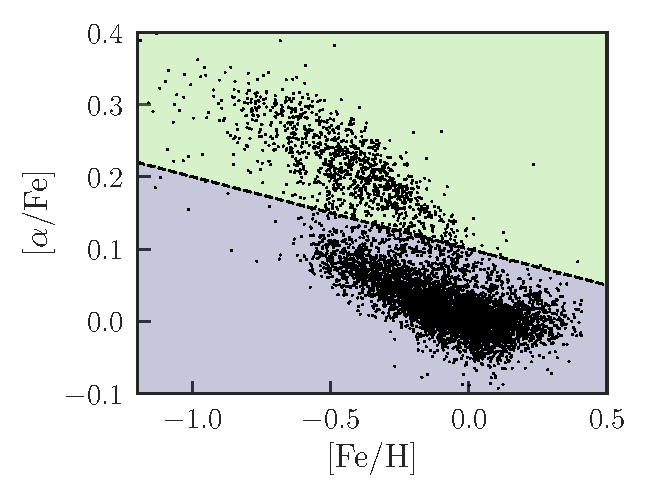
\includegraphics[width=0.8\textwidth]{thesis/Plots/afe_split_colors.pdf}
    \caption[The \feh{} and \afe{} abundances of stars in the solar vicinity from APOGEE DR14, indicating the bimodality in \afe{} at fixed \feh{}]{The \feh{}-\afe{} plane for stars located near the Sun (within 1 kpc) from the fourteenth data release (DR14 of the APOGEE survey). The coloured regions indicate a rough selection of stars with high (\emph{green}) and low (\emph{blue}) \afe{}. A bimodality in \afe{} is clearly present, at fixed \feh{}, between $-0.5 \lesssim \mathrm{[Fe/H]} \lesssim 0.0$ dex. The two populations appear to overlap at roughly solar \feh{}.}
    \label{fig:afe_split}
\end{figure}

These populations have, of course, been studied extensively since their discovery \citep[e.g.][]{1998A&A...338..161F,2003A&A...410..527B,2005A&A...433..185B,2013A&A...560A.109H,2014A&A...562A..71B,2014A&A...564A.115A,2014ApJ...796...38N,2015ApJ...808..132H} and, as expressed in Section \ref{sec:disksize}, have important links to the spatial structure of the Galaxy. Along with the MDFs (mentioned above), large scale spectroscopic surveys have also unveiled the stellar \feh{}-\afe{} distribution over great extents of the disk.  \citet{2014ApJ...796...38N} demonstrated that the positions of Red Clump (RC) stars (whose distances can be accurately measured by the fact that they are standard candles) in \feh{}-\afe{} space change as a function of Galactocentric radius and height. \citet{2015ApJ...808..132H} followed up on that work by showing a similar trend in a much larger sample Red Giant Branch stars. The findings of both studies were that that the mean \feh{} of the low \afe{} stars appears to move to higher \feh{} at smaller $R$, while the high \afe{} stars dominate the distribution at high $z$, and occupy a similar locus everywhere in the disk but appear to decline in density with $R$. These results place very strong constraints on any model which hopes to explain the origin of these element abundance trends, and I will briefly discuss such models in Section \ref{sec:galacticarchaeology}.

\subsection{The Bulge and Bar}

I discuss the bulge of the Milky Way in coordination with the bar, as these components are co-spatial in the center of our Galaxy and have a history and origin which is likely linked in some way, at some point in time.

\subsubsection{Classical or \emph{pseudo}-bulge?}
During the early years of studying the Milky Way bulge, there was much debate as to its origin. The main arguments were either that it built up in the early history of the Galaxy through the merging of its satellite galaxy progenitors -- and thus is a `classical' bulge, resembling the structure of elliptical galaxies, which are thought to be built by the same process -- or that it formed in a secular fashion from stars in the disk or bar of the galaxy to become a `pseudobulge' \citep[a useful summary of these definitions is provided in Section 1.1 of][]{2004ARA&A..42..603K}. There now exists a wealth of evidence to suggest that while external galaxies certainly do host classical bulges \citep[e.g.][]{2009MNRAS.393.1531G}, the Milky Way itself is more likely host to a bulge with a structure indicative of secular processes - a pseudobulge. The Galactic bulge is boxy in shape \citep[e.g][]{1995ApJ...445..716D}, and is proposed to be formed via the heating of stars by buckling of a bar which formed from the stellar disk \citep[e.g.][]{1981A&A....96..164C,1991Natur.352..411R}.



\subsubsection{Unveiling the bar}


\subsection{The Halo}

\subsection{The Local Group}

\section{Galactic archaeology: fossilised galaxy formation}
\label{sec:galacticarchaeology}
\subsection{A schematic for the formation of disk galaxies}

A useful way to present the wealth of work on the formation of the Milky Way is to describe a schematic of its formation as a disk galaxy, as unveiled by studies of it throughout the last century. The conception of the `canonical' model for the birth of the Milky Way in a rapid collapse of a proto-galactic gas cloud \citep[the ELS model;][]{1962ApJ...136..748E} makes a good starting point for such a schematic. 

In what can be considered as the first implementation of Galactic archaeology, \citet{1962ApJ...136..748E} showed that the orbital energies and eccentricities of stars with lower metallicities were increased, inferring that these stars were members of the first generation of stars formed from the originally rapidly collapsed protocloud of our galaxy. The later work of \citet{1978ApJ...225..357S}, which inferred that the varying element abundances of Galactic globular cluster (GC) systems, suggested a different view of the formation of the galaxy through the conglomeration of `protogalactic fragments'. These seminal works underpin many of the modern studies of the Milky Way, and are commonly framed as competitive scenarios. However, at the time, these findings mirrored the developments in the CDM model \citep{1978MNRAS.183..341W}, and analytical models of the collapse of gas in a halo which gained angular momentum from hierarchical clustering produced seemingly realistic disks \citep{1980MNRAS.193..189F}. While analytic approaches would work well at describing galaxy disk formation, hydrodynamical simulations in a cosmological context struggled to produce realistic populations of disk galaxies until advances in the inclusion of detailed feedback models, as expressed in Section \ref{sec:galaxyhaloconnect}. 




\chapter{The age-resolved spatial structure of the Milky Way disc}
\label{chapter:apogeestruc}
\section{Introduction}

As has already been discussed in Chapter \ref{chapter:intro}, understanding of the present day spatial, kinematic and chemical configuration of the stars of the Milky Way disc is a cornerstone of Galactic archaeology, placing key constraints on models of galaxy disc formation and evolution. Much of our understanding of the time evolution of galaxy discs like that of the Milky Way has arisen from studies which match galaxies of a given stellar mass at $z=0$ to their progenitors at higher $z$ \citep[and therefore, lookback time, e.g.][]{2013ApJ...771L..35V,2015ApJ...803...26P,2016MNRAS.462.4495H}. 
%However, the Sun's position in the Milky Way presents a high-fidelity insight into the structure of a Galactic disc on a star by star basis, which has provided a great many insights into the problem \citep[e.g.][]{1962ApJ...136..748E,1993A&A...275..101E,2013A&A...560A.109H}. 
Data for large numbers of disc stars over a wide range of Galactocentric distances, including positions, chemical abundances and stellar ages are now readily available, due to the advent of modern spectroscopic surveys such as APOGEE \citep{2015arXiv150905420M}, Gaia-ESO \citep{2012Msngr.147...25G} and GALAH \citep{2016arXiv160902822M}, with many future instruments planned, such as WEAVE \citep{2014SPIE.9147E..0LD} and MOONS \citep{2012SPIE.8446E..0SC}, aiming to bolster the revolutionary data releases from \emph{Gaia} \citep{2016A&A...595A...1G}.

In Section \ref{sec:discsize}, I touched upon the definition of the disc population being measured in the Galaxy appears to have a great effect on estimates of it's structure. Thicker stellar populations, defined geometrically have generally flatter radial profiles with larger scale lengths \citep[e.g.][]{2008ApJ...673..864J} than, for example, the populations enhanced in $\alpha$-element abundances \citep[e.g.][]{2012ApJ...752...51C,2012ApJ...753..148B,2016ApJ...823...30B}. Theoretical results have suggested that such \emph{geometric} thick discs are formed from embedded flaring of co-eval populations  \citep{2015ApJ...804L...9M}. The finding of a radial age gradient above the midplane in the disc \citep[e.g.][]{2016arXiv160901168M}, provides further evidence that the \emph{geometric} thick disc is likely to really be a combination of young and flared, and old, centrally concentrated and thick, populations \citep[as predicted by the models of][]{2015ApJ...804L...9M}.

% When considered \emph{in toto}, nearby galaxy discs, and the Milky Way disc, are observed to have a two-component vertical spatial structure, commonly referred to as the \emph{geometric} `thick' and `thin' discs \citep{1979ApJ...234..842T,1979ApJ...234..829B,1982PASJ...34..365Y,1983MNRAS.202.1025G,2008ApJ...673..864J}. Classically, the `thick' components have been characterised by older, kinematically hotter stellar populations, enriched in \afe{}, whereas the `thin' populations assume lower, near solar \afe{} and are kinematically cooler \citep[e.g.][]{2005A&A...433..185B}. It has, however, also been posited that these populations are in fact composed of multiple sub-populations that smoothly span this range of properties \citep[e.g.][]{1987ApJ...314L..39N,1991PASP..103...95N,2012ApJ...755..115B,2012ApJ...753..148B,2016ApJ...823...30B}, thus, in terms of structural parameters, the disc cannot be characterised as the superposition of two distinct structures with different scale heights \citep{2012ApJ...751..131B}. It has been shown  that the total vertical stellar spatial distribution resulting from the overlap of such sub-populations is consistent with a double exponential \citep[see, e.g., Figure 14 of][]{2013A&ARv..21...61R}. It is difficult to explain the presence of a continuity in structure alongside the discontinuity in chemistry seen in the Milky Way.

The Milky Way disc has a complex chemical structure which connects to its spatial structure in a seemingly complex way, with a bimodality in \afe{} seen at fixed \feh{} across many of the observable regions of the disc, that changes in nature with Galactocentric radius and height above the midplane \citep{2003A&A...410..527B,2005A&A...433..185B,2014ApJ...796...38N,2015ApJ...808..132H}. This characteristic feature, and its spatial variation, is difficult to explain using one-zone Galactic chemical evolution (GCE) models \citep[most recently shown by][]{2016arXiv160408613A}, giving rise to attempts to explain it by means other than pure chemical evolution. Examples of such models include the heating of an old, high-\afe{} disc by high redshift mergers \citep[e.g.][]{2004ApJ...612..894B,2008MNRAS.391.1806V,2009ApJ...700.1896K,2013A&A...558A...9M} and the formation of a dual disc by gradual accretion of stars into disc orbits \citep[e.g.][]{2003ApJ...597...21A}. More recent work has also framed this bimodality as a consequence of discontinuous radial migration of stars in the disc \citep{2016arXiv161009869T}. While this chapter examines the structure of the high and low-\afe{} components, I will return to this feature in Chapter \ref{chapter:eagle}.

% However, such chemical structure can be replicated in part by invoking various Galactic chemical evolution models that do not rely on a `one-zone' approximation \citep[e.g.][]{1997ApJ...477..765C,2000A&A...355..929P,2016arXiv160408613A,2016arXiv160407435W}. For example, \citet{2016arXiv160408613A} showed that a combination of GCE models with varying outflow mass loading parameters and inflow timescales (intended to represent enrichment histories at varying Galactocentric radii) could make a roughly bimodal \afe{} distribution. The same models were shown to present a good explanation of the APOGEE \afe{}-\feh{} plane by \citet{2014ApJ...796...38N}. A deeper understanding of the connection between spatial structure in \afe{} and stellar age selected populations in the Milky Way is necessary to link these results. 

 In this chapter, I present the first dissection of radially extended samples of Milky Way disc stars in age, \feh{} and \afe{}. A strong correlation is observed between stellar age and \afe{} in the solar vicinity \citep{2013A&A...560A.109H}. On the other hand, but also in the solar vicinity, a very large scatter is found around the correlation between age and [Fe/H] \citep[e.g.][]{1993A&A...275..101E,2004A&A...418..989N}. This scatter may be explained by the occurrence of radial migration of stars formed in different disc regions. Thickening of the Galactic disc has been invoked as a consequence of outward stellar radial migration \citep[e.g.][]{2009MNRAS.399.1145S}. However, \citet{2012A&A...548A.127M} argue that the effect is small and that such migration in fact only makes discs flare by a small amount. Similarly, \citet{2016ApJ...823...30B} measured the flaring profile of low-\afe{} stars to only slowly exponentially increase with Galactocentric radius, and suggest that radial migration is likely not a viable mechanism for forming thickened disc components. Flaring has also been shown to arise as a result of satellite infall, which can be a stronger flaring agent than migrations \citep[e.g.][]{2009ApJ...707L...1B}. The understanding of flaring and its connection to the evolution of the Galactic disc is essential, but as yet incomplete. In this chapter, I present new constraints on models of radial migration in the disc by studying its effects on the Milky Way's mono-age stellar populations. 

 Many theoretical studies have attempted to understand the observed structure of mono-abundance populations (MAPs) through the use of hydrodynamics and N-body simulations. Few reproduce the observed bimodality in \afe{} at fixed \feh{}, and so an understanding of this has so far proved difficult. However, certain characteristics of the Milky Way \afe{} distribution are beginning to emerge in the most recent cosmological simulations  \citep{2016arXiv160804133M}. Structurally, the mono-age populations of simulated galaxies show good agreement with the Milky Way \citep[e.g.][]{2013MNRAS.436..625S,2013ApJ...773...43B,2014MNRAS.442.2474M,2014MNRAS.443.2452M}. More recent work has brought into question the applicability of MAPs as a proxy for mono-age populations \citep{2017ApJ...834...27M}, showing that, particularly at low-\afe{}, MAPs may have significant age spreads due to the differential nature of star formation in the disc. I show in this chapter that the structures of mono-age and mono-\feh{} populations in the low and high-\afe{} Milky Way disc components present insights which are complementary to those of the MAPs, into the temporal and chemical evolution processes in the disc.

 Previous work studied MAPs in the Milky Way by analysing samples of SEGUE G-dwarfs \citep{2012ApJ...755..115B,2012ApJ...753..148B,2012ApJ...751..131B} and APOGEE red-clump (RC) giants \citep{2016ApJ...823...30B}. In this chapter, I map the spatial distribution of mono-age, mono-\feh{} populations at low and high-\afe{} using a catalogue containing \feh{} and \afe{} from the twelfth data release (DR12) of the APOGEE survey \citep{2015arXiv150905420M} and ages from \citet{2016MNRAS.456.3655M} for 31,244 red giant stars. I complement earlier work by adapting the method developed by \citet{2016ApJ...823...30B} for RC stars, to enable its application to the full red giant branch (RGB) sample from APOGEE. Stars in the RGB are better tracers of the underlying stellar population than their RC counterparts because of reduced uncertainties in the stellar evolution models. Additionally, because they are generally brighter, they are also observed at greater distances. On the other hand, this means that the method developed by \citet{2016ApJ...823...30B} must be adapted to account for the spread in absolute magnitude over the RGB (whereas RC stars can be considered as a near-standard candle). On the basis of these measurements, I will establish the local mass-weighted age-\feh{} distribution, showing the contributions from both low and high-\afe{} stellar populations.

 In Section \ref{sec:dataa}, I present the APOGEE DR12 data and the distance and age catalogues used for this work. Section \ref{sec:methoda} describes the stellar density fitting method, drawing greatly on work by \citet{2016ApJ...818..130B,2016ApJ...823...30B}. Specifically, I describe the generalities of the maximum likelihood fitting procedure and the calculation of the effective survey selection function for RGB stars in Section \ref{sec:densfit}, the adopted parametric stellar density model in Section \ref{sec:densitymodel}, and the method for calculating stellar surface-mass densities in Section \ref{sec:surfmasscalc}. I present the fitted models in Section \ref{sec:resultsa}, calculating the surface-mass density contributions for each mono-age, mono-\feh{} population. In Section \ref{sec:discussiona} I compare these findings to those in the literature and discuss possible scenarios for the formation of the Milky Way's disc in light of these novel results. Section \ref{sec:conclusionsa} summarises the results and conclusions from this chapter. 


 \section{Data}

\label{sec:dataa}
 \subsection{The APOGEE Catalogue}
 \label{sec:APOGEE}
For this chapter, I use data from the twelfth data release \citep[DR12,][]{2015ApJS..219...12A} of the SDSS-III APOGEE survey \citep[][]{2015arXiv150905420M}, a high signal-to-noise ratio (SNR$>100\ \mathrm{pixel}^{-1}$), high resolution ($R \sim 22,500$), spectroscopic survey of over 150,000 Milky Way stars in the near-infrared $H$ Band ($1.5 - 1.7 \mathrm{\mu m}$). Stars were observed during bright time with the APOGEE spectrograph \citep{2010SPIE.7735E..1CW} on the 2.5m Sloan Foundation Telescope \citep{2006AJ....131.2332G} at Apache Point Observatory. Targets were selected in general from the 2MASS point-source catalog, employing a dereddened $(J-K_S)_0 \geq 0.5$ colour cut (in the fields which are of interest here) in up to three apparent $H$ magnitude bins \citep[for a full description of the APOGEE target selection, see][]{2013AJ....146...81Z}. Reddening corrections were determined for the colour cut via the Rayleigh-Jeans Colour Excess method \citep[RJCE,][]{2011ApJ...739...25M}. Corrections are found by applying the method to 2MASS \citep{2006AJ....131.1163S} and mid-IR data from \emph{Spitzer}-IRAC GLIMPSE-I, -II, and -3D \citep{2009PASP..121..213C} when available and from WISE \citep{2010AJ....140.1868W} otherwise. For this work, distance moduli (which make use of the aforementioned reddening corrections) are taken from the \citet{2015ApJ...808..132H} distance catalogue for DR12 (see Section \ref{sec:distances}). 

 All APOGEE data products employed in this paper are those output by the standard data reduction and analysis pipeline used for DR12. The data were processed \citep{2015AJ....150..173N}, then fed into the APOGEE Stellar Parameters and Chemical Abundances Pipeline \citep[ASPCAP,][]{2016AJ....151..144G}, which makes use of a specifically computed spectral library \citep{2015AJ....149..181Z}, calculated using a customised $H$-band line-list \citep{2015ApJS..221...24S}. Outputs from ASPCAP are analysed, calibrated and tabulated \citep{2015AJ....150..148H}. The output \afe{} and \feh{} abundances for DR12 have been shown to have a high degree of precision (at least between $4500 \lesssim \mathrm{T_{\mathrm{eff}}} \lesssim 5200$ K), such that $\sigma_{\mathrm{[Fe/H]}} = 0.05\ \mathrm{dex}$ and $\sigma_{\mathrm{[\alpha/Fe]}} = 0.02\ \mathrm{dex}$ \citep{2016ApJ...823...30B}. I apply here the same external calibrations to \afe{} and \feh{} as \citet{2016ApJ...823...30B}: constant offsets of -0.05 dex and -0.1 dex, respectively. The calibrated, tabulated \feh{} value is used rather than the globally fit $\mathrm{[M/H]}$, which is included in the table.

I then select stars from the DR12 catalogue which were targeted as part of the main disc survey (i.e were subject to the $(J-K_S)_0 \geq 0.5$ cut), have reliably measured abundances (i.e. no warning or error bits set in the ASPCAPFLAG field) and have a well defined distance modulus and age measurement (see Sections \ref{sec:distances} and \ref{sec:ages}, for specific discussion of the age and distance catalogues employed). I apply a secondary cut at $1.8 < \log{g} < 3.0$ to restrict the sample to stars on the red giant branch (RGB), removing most contaminating dwarfs, and very evolved stars near the tip of the RGB. The high end of our $\log{g}$ cut is more conservative than other studies in this regime, however I find this gives the best agreement between the data and stellar evolution models, without significantly reducing the sample size or introducing unwanted bias. These cuts give a final sample of 31,244 stars, spanning $4200 \lesssim \mathrm{T_{\mathrm{eff}}} \lesssim  5050\ \mathrm{K}$ for which the effective survey selection function can be reconstructed.

I further divide the sample into low and high-\afe{} sub-samples, as it has been shown in previous work that the two populations have quite different structural parameters \citep{2016ApJ...823...30B}, and as such it makes sense to proceed to fit their mono-age, mono-\feh{} sub-populations separately. I visually separate the low and high-\afe{} populations, leaving a gap between the two samples of 0.05 dex in \afe{} at each \feh{} (this separation is shown in Figure \ref{fig:afe_feh}), minimising contamination between the subsamples, particularly at the high \feh{} end, where the two populations partially overlap, and at the low \feh{} end, where \afe{} errors become enlarged. The final density fits are performed on finer bins in age and \feh{}, which is defined in Section \ref{sec:ages}. As the adopted separation in \afe{} removes 6532 stars from the full count, when calculating the surface-mass density contributions from the stellar number counts in each age-\feh{} bin, I remove the separation in \afe{}, using the star counts as if the populations were separated along the midpoint of the division (as shown by the dot-dashed line in Figure \ref{fig:afe_feh}). 

 \begin{figure}
  \centering
 	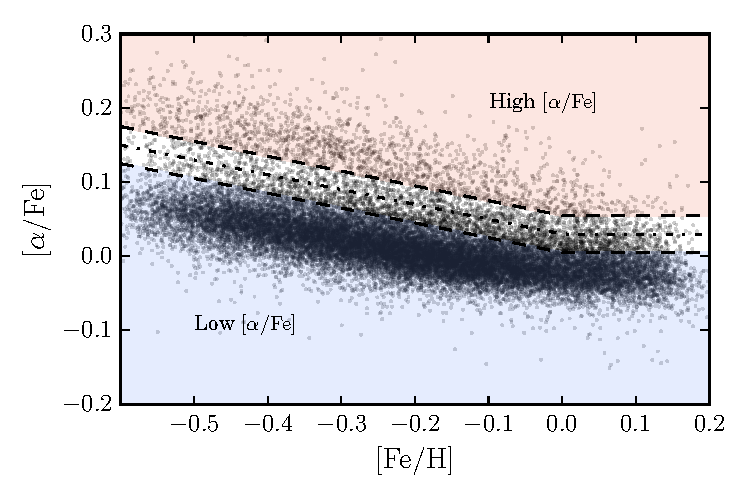
\includegraphics[width=0.7\columnwidth]{afe_feh_subsamples.pdf}
    \caption[\afe{}--\feh{} for the APOGEE DR12 sample, demonstrating the division used to divide between high and low-\afe{} populations in Chapter \ref{chapter:apogeestruc}]{The full APOGEE DR12 RGB sample in \afe{}--\feh{} space. The coloured regions show the division between low and high-\afe{} subsamples used for the DR12 dataset, which is determined by eye to best divide the two populations at the low \feh{} end. At each \feh{} the division between the samples is \afe{} $= 0.05 \ \rm{dex}$, roughly twice the mean uncertainty on \afe{} abundance determinations in APOGEE DR12. The bimodality in \afe{} at fixed \feh{} is visible across many \feh{}, and the lower number of stars in the high-\afe{} sample is clear from this plot. Figure \ref{fig:afe_split} shows a similar sample using the DR14 data, which will be used in Chapter \ref{chapter:highe}.}
 \label{fig:afe_feh}
\end{figure}


The method used to model the spatial density of the mono-age, mono-\feh{} populations, discussed in Section \ref{sec:methoda}, corrects for selection effects induced by interstellar extinction (in addition to the RJCE reddening corrections) using 3D dust maps for the Milky Way derived by \citet{2006A&A...453..635M} for the inner disc plane, combined with those for a large majority of the APOGEE footprint by \citep{2015ApJ...810...25G}, adopting conversions $A_H/A_{K_S}=1.48$ and $A_H/E(B-V) = 0.46$ \citep{2011ApJ...737..103S,2013MNRAS.430.2188Y}.  Fields with no dust data (of which there are $\sim 10$) are removed from the analysis. \citet{2016ApJ...823...30B} discuss the relative merits and limitations of these dust maps as opposed to others which are available, and determine that this combination of dust maps provides the best density fits.


 \subsection{Distance estimates}
 \label{sec:distances}
 
  \begin{figure}
 \centering
 	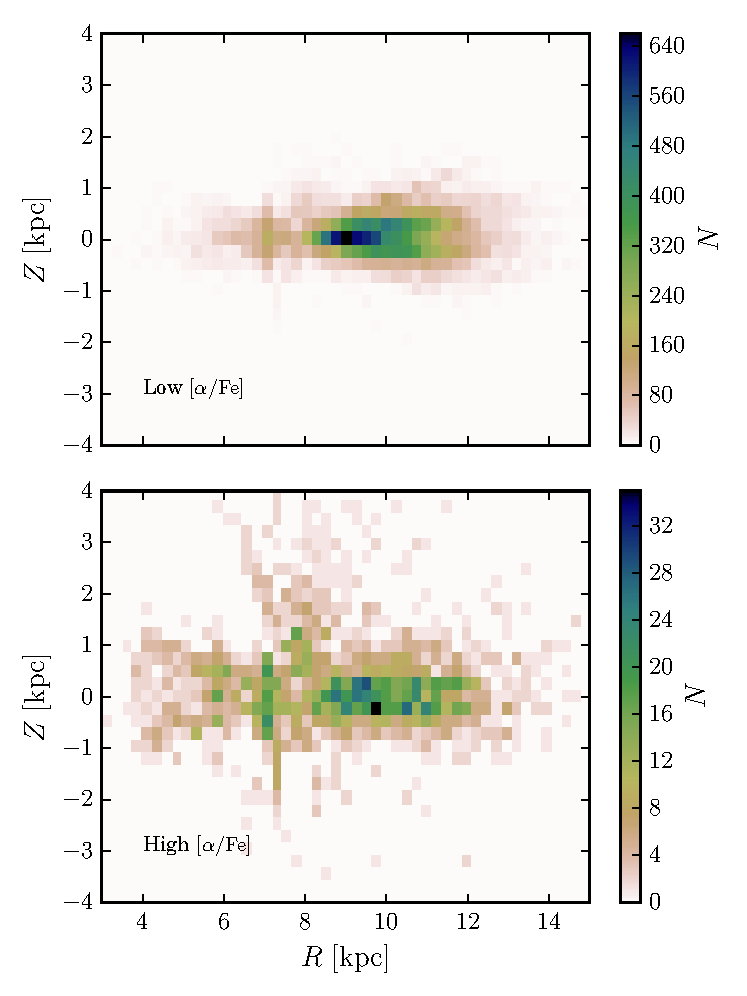
\includegraphics[width=0.8\columnwidth]{spatial_clean_subsamples_binned.pdf}
     \caption[The Galactocentric $R$ and $z$ distribution of stars in the APOGEE DR12 high and low-\afe{} populations]{2D histograms of the spatial distribution (in Galactocentric $R$ and $Z$) of the high and low-\afe{} subsamples from APOGEE DR12, shown in Figure \ref{fig:afe_feh}. The high-\afe{} sample appears more diffuse and extended in height even before selection effects are accounted for. Readers should notice the different colour scale adopted for each panel, due to the much lower number of stars in the high-\afe{} sample.}
     \label{fig:spatial}
 \end{figure}
In this chapter, I use distance estimates from \citet{2014AJ....147..116H} \citep[But see also][for further description]{2015ApJ...808..132H}. Distances are estimated by computing the probability distribution function (PDF) of all distance moduli to a given star using a Bayesian method applied to the spectroscopic and photometric parameters from the DR12 catalogue and the PARSEC isochrones \citep{2012MNRAS.427..127B}. The distance estimates are found to have accuracy at the $15-20\%$ level, upon comparison with cluster members of well known distance observed by APOGEE. 

I use the median of the posterior PDF (which is given in the output catalogue) as the estimate for the distance modulus, and compute the Galactocentric cylindrical coordinates, $R, \phi\ \rm{and}$  $Z$ for each star using the $l,b$ coordinates provided in the APOGEE-DR12 catalogue. The spatial distribution of the two \afe{} sub-samples is shown in Figure \ref{fig:spatial}. I perform a simple cross match between our sample and the APOGEE red clump (RC) value added catalogue (VAC) \citep{2014ApJ...790..127B} and plot the red-clump derived distance ($D_{RC}$) against the estimate from \citet{2014AJ....147..116H} ($D_{MH}$) in Figure \ref{fig:distcomp}. The majority of the \citet{2014AJ....147..116H} distances compare well to the RC distances, but there are notable differences. The \citet{2014AJ....147..116H} distances can be underestimated by as much as 50\%, and I find that $\sim20\%$ of the sample have distances which are underestimated by more than 10\%. Our density fitting method is insensitive to uncertainties on the distances at these scales, as the scale of any variations in the density distribution can be assumed to be far greater than the distance uncertainties. 

 Figure \ref{fig:distcomp} also shows that there is a systematic offset between the RC and \citet{2014AJ....147..116H} distances of the order $\sim 5\%$ across the full range of distances. Adopting this offset as a correction to the distances makes little impact on the final results, merely broadening fitted density profiles slightly, spreading the star counts over a wider Galactocentric distance, meaning that the final stellar surface-mass density estimates are unchanged.

\begin{figure}
 	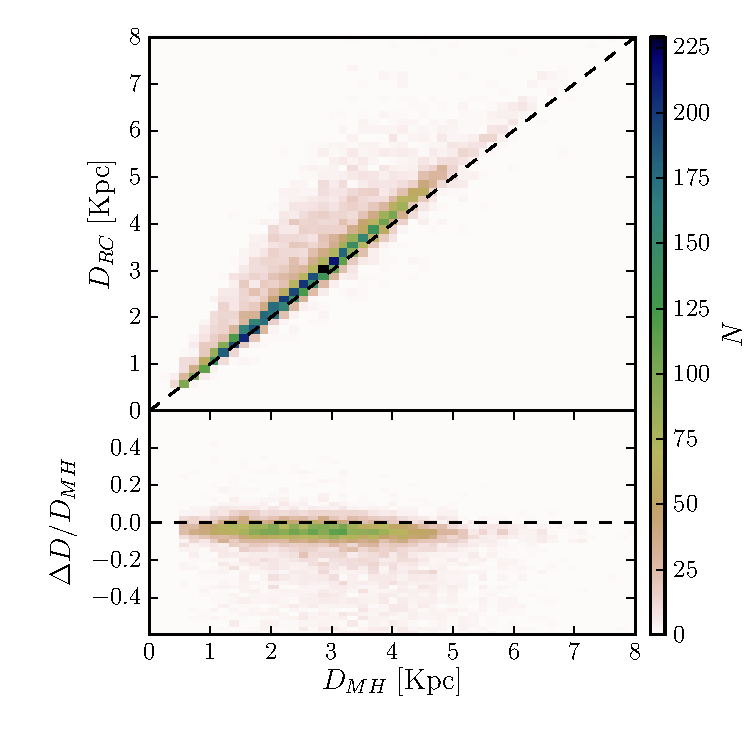
\includegraphics[width=0.8\columnwidth]{distancecomparison_binned.pdf}
    \caption[Comparison of APOGEE RC catalogue distances with distances derived by \citet{2015ApJ...808..132H}, as used in Chapter \ref{chapter:apogeestruc}]{Comparison of APOGEE red clump catalogue (APOGEE-RC) distances $D_{RC}$ with distances derived by \citet{2015ApJ...808..132H}, $D_{MH}$. The top panel directly compares the distances, where the bottom panel shows the difference as a fraction of $D_{MH}$, as a function of that distance.  There are many stars with good agreement, but a distinct fraction of MH distances are underestimated compared to RC ($\sim 20\%$ with distances underestimated by more than $\sim 10\%$). As the variations in the density occur on scales which are, in general, far larger than these discrepancies, these are not problematic in our analysis. The two distance scales differ systematically by a factor of $\sim 5\%$, but this is not corrected for in the following discussion and it does not impact any of the general results.}
    \label{fig:distcomp}
 \end{figure}

Given that stellar distances are rapidly being improved by the \emph{Gaia} mission, it is likely that the precision on stellar distance estimates can now be improved, particularly for stars very close to the sun. However, it is expected that even with parallax information for the stars, the distance estimates to the furthest stars in this sample would likely still be subject to uncertainties of $\sim 5$ to $10\%$ until the highest precision parallaxes become available with the end-of-mission \emph{Gaia} data releases. Given, as I have already pointed out, that the stellar density (which is fitted here) varies on scales far greater than the distance uncertainties, it could be expected that improved precision on distances would only marginally improve the precision and accuracy of the results found here.

 \subsection{Age estimates}
 \label{sec:ages}
I use age estimates for APOGEE DR12 estimated by \citet{2016MNRAS.456.3655M}, who derive an empirical model for the $\mathrm{[C/N]} -M_*$ relation using asteroseismic masses from \emph{Kepler} and abundances from APOGEE for their overlapping samples \citep[APOKASC ][]{2014ApJS..215...19P}. Masses are predicted for DR12 stars which meet quality and stellar parameter criteria outlined in \citet{2016MNRAS.456.3655M}, and ages are estimated from that mass using the PARSEC isochrones with the nearest metallicity to that of the given star. \citet{2016MNRAS.456.3655M} use this empirical relation to build a model which predicts mass and age as a function of $[\text{[M/H], [C/M], [N/M], [(C+N)/M],}\log{g},T_{\mathrm{eff}}]$. It is important to note here that \citet{2016MNRAS.456.3655M} derive a model and fit for the ages in DR12 using the uncalibrated, raw stellar parameters, found in the FPARAM arrays in the APOGEE catalogue. This is difficult to account for when using the age catalogue alongside the calibrated parameters, and must be borne in mind in future comparisons of this work with models and observational results. In addition to this, \citet{2016MNRAS.456.3655M} also mention that care should be taken when applying these ages to regions of the Milky Way where the chemical evolution may have been complex (e.g. the Bulge/Bar region). However, in their Figure 12, they compare the [C/N] ratio as a function of [M/H] in a sample of pre-dredge-up giants in the inner and outer disc, showing that the shapes of the distributions are similar. This suggests that differences in chemical evolution do not affect the $\mathrm{[C/N]}$-age relation within a wide range of galactocentric distances. Therefore, the assumption that it is safe to adopt the \citet{2016MNRAS.456.3655M} ages over the extent of the disc covered by our sample is robust, regardless of the fact that they are trained on the \emph{Kepler} sample, which is limited in its spatial extent.

 Although individual uncertainties on ages are not given in the catalogue, \citet{2016MNRAS.456.3655M} state that the model predicts ages with r.m.s errors of $\sim 40\%$. Although uncertainties are potentially very large at high age, the sample used here is binned with $\Delta \text{age}= 2$ Gyr in order to gauge general trends with age. It should be understood that such trends are smoothed by the age uncertainties, particularly at high age, and detailed comparisons to models should take this age uncertainty into account. I discuss the effect of these uncertainties on our recovered trends with age in Appendix \ref{sec:ageerror}, and show that the methodology still reliably recover such trends with age, even though mixing between bins may be present in the data.

 Figure 11 of \citet{2016MNRAS.456.3655M} shows that there is a significant bias in the ages returned by the model, such that ages are underpredicted at high age when compared to the training set. For this reason, I fit for and apply a correction to the catalogued ages before performing the density fitting procedure. Using Table 1 from \citet{2016MNRAS.456.3655M}, I perform a non-parametric lowess fit to the predicted age--true age distribution. This fit is then used to derive age corrections as a function of predicted age. The fitted correction is shown in Figure \ref{fig:correction} in both predicted vs. true age space and also in $\Delta$ age against the predicted age. The correction as a function of predicted age is then applied to each of the ages in the DR12 catalogue. In all further analysis, I refer only to the corrected ages. The main effect of this correction is to make the high-\afe{} stars older. Consequently, our surface-mass density estimates (presented in Section \ref{sec:surfmassdens}) become more conservative, as the mass contribution per star in older bins is lower (as discussed in Section \ref{sec:discrepant}). \citet{2016MNRAS.456.3655M} comment on the bias in the context that the ages returned for high-\afe{} stars appear younger than previous estimates \citep[from][]{2013A&A...560A.109H,2014A&A...562A..71B,2014A&A...565A..89B}. This correction brings these data more in line with those estimates.  
 
  \begin{figure}
 	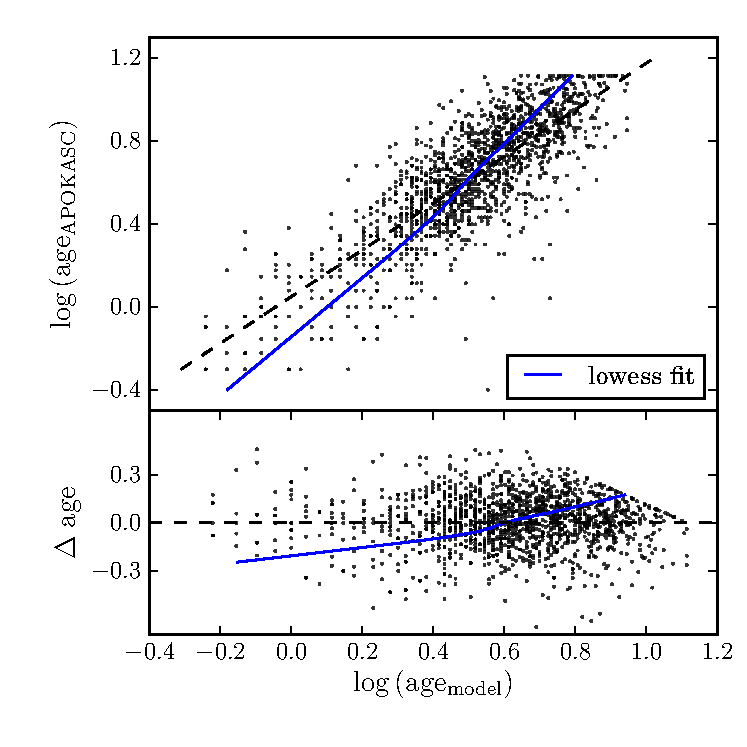
\includegraphics[width=0.8\columnwidth]{agebias_invsout.pdf}
 	\centering
     \caption[Comparison between the input and output ages from \citet{2016MNRAS.456.3655M}, demonstrating the fit and correction which is applied to the age catalogue for APOGEE DR12]{Asteroseismically determined ages from APOKASC against the $\mathrm{[C/M]}$ and $\mathrm{[N/M]}$ based ages from \citet{2016MNRAS.456.3655M}. The line gives the fitted correction for ages from \citet{2016MNRAS.456.3655M}, based on the values for the APOKASC training set, given in their Table 1. The data are fit using a non-parametric lowess fit. Before corrections, older ages are under-predicted, and young ages are over-predicted. The corrections mainly change the scaling of the ages, such that the high-\afe{} sample occupies an age range more in-line with the existing literature \citep[e.g.][]{2016arXiv160407771A,2013A&A...560A.109H} }
  \label{fig:correction}
\end{figure}



 It is also important to account for all other cuts made by \citet{2016MNRAS.456.3655M} on the stellar parameters in the APOGEE catalogue, outlined in full at the beginning of their Section 6.2. While I account for cuts in $T_{\mathrm{eff}}$ and $\log{g}$ by applying the same cuts to the isochrone grid when calculating surface-mass density contributions, it is not possible to properly account for cuts made on the stellar abundances in this way. 9,041 stars are removed from the 40,285 star catalogue (those with distances, after the $\log{g}$ cut mentioned above) by these abundance cuts, to give the final catalogue size of 31,244. This means that $\sim 25\%$ of genuine star counts are missing from the age catalogue, and therefore unaccounted for in the following analysis. With no robust method for determining the age distribution of these missing stars, I make the simplest assumption that these star counts can simply be added uniformly to each age-\feh{} bin. I make this correction by simply increasing the counts in each bin by $25\%$ when calculating the surface-mass density. This correction simply acts to increase the final surface-mass density values systematically by $25\%$.

Another important consideration when using this set of ages regards stars whose chemical compositions are such that the ages fit from the model (after making the corrections) would be higher than 13 Gyr and left out of the analysis. As age estimates are computed based on the surface parameters and abundances of the stars using a fitting function, many stars with strongly outlying abundances and parameters can be assigned ages which are greater than 13 Gyr. I find that the 3020 such stars (in the final sample) have an average [C/Fe] which is lower than the general sample, and an average [N/Fe] which is enhanced with respect to the stars with reliably measured ages. I also find that at fixed \feh{} and $\log{g}$ these stars have warmer $T_{\mathrm{eff}}$. While these properties are expected given their age measurements, there is a distinct possibility of some peculiarity of these stars. For example, if such stars were early AGB stars \citep[having gone through the second dredge-up, reducing the surface C abundance, e.g.][]{1999ApJ...510..232B}, which had been fit as RGB stars, their actual age may be considerably younger, and their counts missed in the younger bins (where mass contribution per star is higher). As the nature of these stars is debatable and a correction cannot be made confidently before carrying out the full analysis, the missing counts from these stars are regarded as a contribution to the systematic error budget, which is discussed fully in Section \ref{sec:discrepant}.

I demonstrate the adopted binning in (age,[Fe/H]) space in Figure \ref{fig:numbins}, showing also the number of stars which fall in each bin and the general distribution of stars in (age,[Fe/H]) space. There is a notable separation in age between the high and low-\afe{} subsamples. 


 \begin{figure}
 	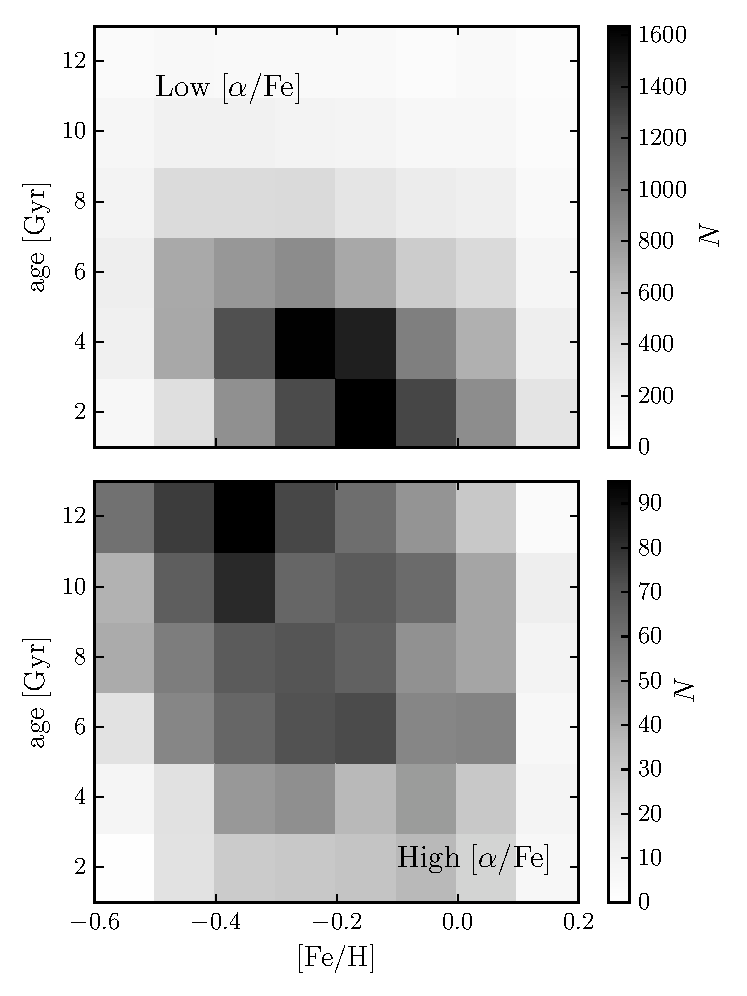
\includegraphics[width=0.8\columnwidth]{agefeh_numbins.pdf}
     \caption[2D Histogram demonstrating the number of stars in each age and \feh{} bin, in the high and low-\afe{} populations, adopted for modelling the stellar density in the disc]{2D Histograms showing the raw number of stars in each (age,\feh{}) bin of the low (\emph{left}) and high (\emph{right}) \afe{} sub-samples. I draw the reader's attention to the difference in amplitude between the two sub-samples (and the associated difference in colour scale normalisation). Although the majority of bins are well sampled ($\gtrsim 30$ stars), there are some greatly undersampled bins, for which well-defined fits are not possible. }
    \label{fig:numbins}
 \end{figure}

 \section{Method}
 \label{sec:methoda}
 In this section I describe the method for fitting the underlying number density of stars in the Milky Way from APOGEE observations, which is represented here as $\nu_*(X,Y,Z|\theta)$, in units of stars kpc$^{-3}$. The calculation of this quantity requires allowances to be made for the survey selection function, which is non-trivial due to the presence of inhomogeneous dust extinction along lines of sight observed by APOGEE, the invocation of different $H$ magnitude limits in the target selection, and the use of RGB stars as a tracer - which cannot be considered as standard candles, as is done for the RC sample. The quantity which I am ultimately interested in is the surface-mass density of stars at the solar radius, $\Sigma_{R_0}$, in units of $\mathrm{M_{\odot}}\ \mathrm{pc^{-2}}$, which I infer here from the number of stars in the APOGEE sample as a function of position. I describe the method for this calculation in Section \ref{sec:surfmasscalc}. The methodology presented here consists of an adaptation of that used by \citet{2016ApJ...823...30B}, employing a modified version of their publicly available code\footnote{Available at \url{https://github.com/jobovy/apogee-maps} - and updated to include the adapted analysis used here}. Although the general method is identical, I describe again the key components for clarity and completeness.

The procedure, described in full below, can be summarised as follows:
  \begin{itemize}
  \item Parametric density models are fit to the APOGEE star counts using a maximum likelihood fitting procedure, based on the assumption that star counts are well modelled as an inhomogeneous Poisson point process. The density models which I assume throughout the remainder of this chapter are described by radially broken exponentials, with scale lengths $h_{R,\mathrm{[in,out]}}$ either side of a break radius $R_{\mathrm{peak}}$ (where $h_{R,\mathrm{in}}$ denotes the scale length of the inner profile and vice versa), and a vertical distribution which is a single exponential with scale height $h_Z$, which is modified as a function of $R$ by an exponential flaring term with scale length $R_{\mathrm{flare}}$. I show that if the density is better fit by a single exponential, it is recovered as so by this procedure.
 \item A best fit density model is obtained for every bin in age and \feh{}, at high and low-\afe{}. This best fit model is then used to initiate an MCMC sampling of the posterior PDF. I then use the median and standard deviation of one dimensional projections of the MCMC chain as our adopted parameter values and uncertainties.
  \item As the fitting procedure does not fit for the normalisation of the density $N_{R_0}$, the number surface density of stars at the solar radius in stars pc$^{-2}$, I calculate this value by comparing the observed number of stars in each bin to that which would be observed in APOGEE for the fitted density model if $N_{R_0} = 1 $ star pc$^{-2}$. The $N_{R_0}$ for each bin is then converted into the surface-mass density in visible stars at the solar radius $\Sigma_{R_0}$ by converting the mass in RGB stars observed to the total mass using stellar evolution models.
 \end{itemize}

 

 \subsection{Density Fitting Procedure}
\label{sec:densfit}
Initially, the number density of stars is fit for each sub-population shown in Figure \ref{fig:numbins}. The following discussion describes the general procedure used for fitting density models with a generic set of parameters $\theta$. The actual stellar number density model adopted is discussed in Section \ref{sec:densitymodel}. \citet{2016ApJ...823...30B,2012ApJ...753..148B,2013A&ARv..21...61R} have shown that the observed rate of stars as a function of position, magnitude, colour and metallicity can be modelled as an inhomogeneous Poisson point process. Stars are distributed in the space defined by $O = [l,b,D,H,\mathrm{[J-K_S]_0}, \mathrm{[Fe/H]}]$ -- position, magnitude, colour and metallicity -- with an expected rate $\lambda(O|\theta)$ (which has units of stars per arbitrary volume unit in O), parameterised by a set of parameters $\theta$ (which are, in this particular case, the parameters describing an adopted density profile). This rate function is written fully as
 \begin{multline}
 \lambda(O|\theta) = \nu_*(X,Y,Z|\theta) \times |J(X,Y,Z;l,b,D)| \\ \times \rho(H, [J-K_S]_0, \mathrm{[Fe/H]}|X,Y,Z) \times S(l,b,H) 
 \label{eq:rate}
 \end{multline}
 where $\nu_*(X,Y,Z|\theta)$ is the quantity being estimated, which is defined as the stellar number density in rectangular coordinates, in units of stars kpc$^{-3}$. $ |J(X,Y,Z;l,b,D)|$ is the Jacobian of the transformation from rectangular $(X,Y,Z)$ to Galactic $(l,b,D)$ coordinates and $ \rho(H, [J-K_S]_0, \mathrm{[Fe/H]}|X,Y,Z) $ denotes the density of stars in magnitude, colour and metallicity space given a spatial position $(X,Y,Z)$, in units of stars per arbitrary volume in magnitude, colour and metallicity space. $S(l,b,H)$ is the survey selection function (the fraction of stars observed in the survey) which includes dust extinction effects, which I will discuss in the following. When expressed in this way, fitting the density model parameters $\theta$ becomes a maximum likelihood problem.

 The likelihood is a sum over all data-points considered in a given age-\feh{} bin, and gives the likelihood of the parameters $\theta$ given the data. For this application, it is written as
 \begin{multline}
 \ln \mathcal{L}(\theta) = \sum_{i} \left[ \ln \nu_{*}(X_i, Y_i, Z_i|\theta)- \ln \int dO \lambda(O|\theta) \right]
 \label{eq:likelihood}
 \end{multline}
 where second term on the right hand side of the equation, $ \int dO \lambda(O|\theta)$, describes the effective volume of the survey. I drop the other factors in the rate in Equation (\ref{eq:rate}) in the argument of the logarithm, because the other factors do not depend on the model parameters $\theta$. The effective volume is independent of the data-point considered, and is an intrinsic property of the survey for a given $\theta$. It provides the normalisation for the rate likelihood, and is non-trivial to evaluate due to the presence of patchy dust extinction along lines of sight in the survey.

 The effective volume is written generally as
  \begin{multline}
 \label{eq:effvol}
 \int dO \lambda(O|\theta) = \sum_{\text{fields}} \Omega_f \int dD D^2 \nu_*([X,Y,Z](D,\text{field})|\theta)\\ \times \mathfrak{S}(\text{field},D)
 \end{multline}
 which is a sum over all APOGEE fields, where $\Omega_f$ is the solid angle of the field considered. The integrand $ \nu_*([X,Y,Z](D,\text{field})|\theta)$ is the density at each point along a line of sight, assumed to be constant over the angular size of the field. $\mathfrak{S}(\text{field},D)$ represents the effective survey selection function, which is given by the integration of the survey selection function over the area of any given field and is written, in this case, as
 \begin{multline}
 \mathfrak{S}(\text{field}, D) = \sum_k S(\text{field},k) \\ \int dM_H \frac{\Omega_k(H_{\text{[min,max]},k}, M_H, A_H[l,b,D], D)}{\Omega_f}.
 \label{eq:effsel}
 \end{multline}
 This is a sum over the apparent magnitude bins, $k$, in the APOGEE target selection, with the integral representing the fractional area of the APOGEE field where stars are observable, given the distance modulus and extinction at a given position. The term describing this area is $\Omega_k$, which is the observable area of the field at a given distance and absolute magnitude, written as
 \begin{multline}
 \Omega_k(H_{\text{[min,max]},k}, M_H, A_H[l,b,D], D) =\\ \Omega(H_{\text{min},k} - [M_H - \mu(D)] < A_H(l,b,D) < H_{\text{max},k} - [M_H - \mu(D)])
 \end{multline}
 where $H_{\text{[min,max]},k}$ denotes the minimum and maximum $H$ for an apparent magnitude bin $k$ in the APOGEE target selection and $\mu(D)$ is the distance modulus at $D$.  $A_H(l,b,D)$ is the $H$ band extinction at a given position, which I obtain from the 3D dust maps described in Section \ref{sec:APOGEE}. This area is integrated (in Equation (\ref{eq:effsel})) over the full absolute $H$-band magnitude, $M_H$, distribution in an (age,\feh{}) bin. I estimate the $M_H$ distribution for each (age,\feh{}) bin using the PARSEC isochrones \citep{2012MNRAS.427..127B} within that bin, weighted with a \citet{2003PASP..115..763C} IMF. The same cuts in $\log{g}$ and $(J-K_S)_0$ colour are applied to the isochrone points as are imposed on the data, and perform a Monte Carlo integration using the resulting $M_H$ distribution to evaluate the integral in Equation (\ref{eq:effsel}). S(\text{field},k) in Equation (\ref{eq:effsel}) denotes the 'raw' APOGEE selection function, which gives the fraction of the stars in the photometric catalogue that were observed spectroscopically \citep[see][for details]{2013AJ....146...81Z}. This number is constant within an apparent magnitude bin and within an APOGEE field, which is why $S$ is cast as a function of field and magnitude bin in Equation (\ref{eq:effsel}). The values of S(\text{field},k) (and $\mathfrak{S}(\text{field}, D)$) are evaluated using the \texttt{apogee} python package \footnote{Available at \url{https://github.com/jobovy/apogee}}.

$\mathfrak{S}(\text{field}, D)$ is then evaluated over a grid of distances for each APOGEE field for simple computation of $\int dO \lambda(O|\theta)$. The likelihood function in Equation (\ref{eq:likelihood}) is then optimised for a given density model and data-set using a downhill-simplex algorithm, to obtain the best fitting set of parameters $\theta$. A Markov Chain Monte Carlo (MCMC) sampling of the posterior PDF is then initiated using this optimal solution. This is implemented with an affine-invariant ensemble MCMC sampler  \citep{goodmanweare2010,2013PASP..125..306F}. All parameter values and associated uncertainties for individiual (age,\feh{}) bins which are reported in the following sections represent the median and standard deviation $\sigma$, respectively, of one dimensional projections of the MCMC chain. 

 \subsection{Adopted stellar number density models}
 \label{sec:densitymodel}
 It was shown in \citet{2016ApJ...823...30B} that density profiles of MAPs are well represented by axisymmetric profiles that can be written as 
\begin{equation}
 \nu_*(R, \phi, Z) = \Sigma(R)\zeta(Z|R) \quad \text{where } \int dZ \zeta(Z|R) = 1.
 \end{equation}
 Furthermore, the exact form of the best fitting profile is that of a radially broken exponential, with a vertical profile that is an exponential with a scale height which varies exponentially with R (a flaring profile), such that
 \begin{equation}
 \ln \Sigma(R) \propto  \begin{cases}
     -h_{R,\text{in}}^{-1}(R-R_0)    & \quad \text{where } R \leq R_{\text{peak}}\\
   -h_{R,\text{out}}^{-1}(R-R_0)  &\quad \text{where } R > R_{\text{peak}}\\
   \end{cases}
 \end{equation}
 and
 \begin{equation}
 \ln \zeta(Z|R) \propto h_Z^{-1} \exp{(R_{\mathrm{flare}}^{-1}[R-R_0])} |Z|-\ln{h_Z(R)}.
 \end{equation}
$R_0$ denotes the solar radius, which I assume here to be 8 kpc. This number only sets the radius at which the profiles are normalised, and so does not have any effect on the fitting procedure. I adopt the same general set of density profiles to describe the mono-age, mono-metallicity populations which are studied here. I bin in \feh{} to account for the observed \feh{} spread at fixed age \citep[e.g.][and our Figure \ref{fig:numbins}]{1993A&A...275..101E}. \citet{2016ApJ...823...30B} also showed that when mock data were fit using the procedure in Section \ref{sec:densfit} and the density profile above, the input parameters were always recovered within acceptable uncertainty ranges. In particular, mock data generated from a single exponential profile was still recovered as such (i.e. with $R_{\mathrm{peak}} = 0$) even when fit assuming a broken exponential profile.

I also note here that this sample is not limited to stars which are members of any specific Galactic component, and as such, may include small numbers of halo stars in the very high-\afe{} and low \feh{} regimes. However, the fitting procedure is agnostic to these contaminants, which would only cause the fits to have larger uncertainty (from the MCMC exploration) about the best fit from the dominant population in a given bin.

\subsection{Stellar surface-mass densities}
 \label{sec:surfmasscalc}
The surface-mass density in visible stars for each of the age and \feh{} populations is computed using the method originally outlined in \citet{2012ApJ...751..131B}. As the fitting procedure does not fit for the normalisation of the density (the surface density is normalised to 1 at $R_0$), I first compute the normalisation $N_{R_0}$, which represents the number density of stars at the solar radius in units of stars pc$^{-2}$ in an (age,\feh{}) bin. $N_{R_0}$ is given by the relation 
\begin{equation}
 N_{R_0} = \frac{N_{*,\text{observed}}}{\int dO \lambda(O|\theta)}
\end{equation}
where $N_{*,\text{observed}}$ is the number of stars observed in the survey for a given (age,\feh{}) and $\int dO \lambda(O|\theta)$ is the usual definition of the effective volume (given by Equation (\ref{eq:effvol})) for a given set of parameters $\theta$, found using the method in Section \ref{sec:densfit}. 

The contribution to stellar surface-mass density is found by first multiplying $N_{R_0}$ by the average mass of a red giant star in the same range of age and \feh{}, given the selection criteria on $\log{g}$ given in Section \ref{sec:APOGEE} (which picks out the RGB) and  $(J-K_S)_0 \geq 0.5$ (given that I only use fields in which this cut was applied).  I then correct this value to represent the total stellar population by dividing by the fractional contribution of the red giants to the total underlying population. These values are found using PARSEC isochrones \citep{2012MNRAS.427..127B}, weighted with a Log-normal \citet{2001ApJ...554.1274C} IMF, as described in the calculation of the effective volume in Section \ref{sec:densfit}. This then leads to a stellar surface-mass density $\Sigma_{R_0}$ as a function of age and \feh{}. The conversion can be expressed as
\begin{equation}
 \Sigma_{R_0}(\mathrm{age,[Fe/H]}) = N_{R_0} \frac{\langle M_{\text{RGB}} \rangle (\mathrm{age,[Fe/H]})}{\omega(\mathrm{age,[Fe/H]})},
\end{equation}
where $\langle M_{\text{RGB}} \rangle (\mathrm{age,[Fe/H]})$ is the mean stellar mass in an (age,\feh{}) bin, and $\omega(\mathrm{age,[Fe/H]})$ is the fraction of stars in the total stellar population in an (age,\feh{}) bin which are within the $\log{g}$ and $(J-K_S)_0$ cuts in APOGEE. The stellar surface-mass density contributions of each bin can then be summed to give the total stellar surface-mass density at the solar radius $\Sigma_{R_0, \text{tot}}$.

The final surface-mass density estimate is strongly dependent on the conversion factors in the above equations, the average RGB star mass, $\langle M_{\mathrm{RGB}} \rangle$, and the fractional contribution from giants, $\omega$. The average giant masses in the range of age and \feh{} used span $0.9 \lesssim \langle M_{\mathrm{RGB}} \rangle \lesssim 2.1 \mathrm{M_{\odot}}$. The most metal poor and oldest populations have the lowest average mass, and the youngest, most metal rich populations have the highest. The fractional contribution from giants in this regime ranges between $0.002 \lesssim \omega \lesssim 0.02 $. The oldest and most metal poor populations have the least giants, whereas the youngest, metal rich populations have the most. These values appear to sit well with recent inventories of the solar neighbourhood, which suggest giants should make up of the order of a few percent of the mass \citep{2015ApJ...814...13M}. I discuss the potential systematics introduced by the use of stellar evolution models in Section \ref{sec:discrepant}.


\section{Results}
\label{sec:resultsa}
I now present results from the density fitting procedure, and the subsequent calculation of the surface-mass density contribution of each mono-age, mono-\feh{} population in Figure \ref{fig:numbins}. Density fitting is performed on all populations, but I only display here the fits for populations with $> 30$ stars, as data below this level become too noisy to render reliable fits. Although the remaining fits can be noisy when star counts are near this limit, this is reflected in the error analysis arising from the MCMC exploration of the posterior PDF of the fitted parameters. I refer the reader to Appendix \ref{sec:densityfits} for a comparison between the data and the fitted models for each mono-age, mono-\feh{} bin, and a qualitative discussion regarding the rationale behind the decision to discuss fits to only the broken exponential density profile described in Section \ref{sec:densitymodel}.

\subsection{The radial profile of mono-age, mono-\feh{} populations}
The fits to the surface density in the low and high-\afe{} sub-samples are shown in Figure \ref{fig:surfdens}. I display fits for all age and \feh{} bins with $> 30$ stars. By shading the profiles by their surface-mass density contribution (as shown in Section \ref{sec:surfmassdens}), I intend to draw the eye to the profiles which contribute most to the mass of the Milky Way disc. I defer a discussion of the individual mass contributions of each bin to Section \ref{sec:surfmassdens}, concentrating in this section on trends in the shapes of the density profiles. 


Although fit with the broken exponential, high-\afe{} profiles are generally better described by near-single exponentials, either showing no break in the radial range, or being fit by a profile with a break at low significance (i.e. a single line could be drawn through the coloured band). Many of the outer profiles (after $R_{\mathrm{peak}}$) in the high-\afe{} sub-sample appear to have a similar slope, suggesting that they may all be represented by the same exponential. The mean outer scale length for the high-\afe{} populations is $h_{R,\text{out}} = 1.9\pm 0.1$ kpc. The picture is noticeably different in the low-\afe{} sub-sample, with profiles showing clear breaks, at well defined radii. Any trends in break radius in this regime are determined with high significance. low-\afe{} profiles have a density which increases with radius out to the break radius, and declines outward of this radius. The fits are not constrained to behave in this way, and this indicates that mono-age, mono-\feh{} populations at low \feh{} are shaped approximately as donut-like annuli. The variation of the break radius then represents the moving peak of stellar density as a function of age and \feh{}. Concentrating on the bins youngest bin ($1 < \mathrm{age} < 3$ Gyr), the break radius is a declining function of metallicity, moving between $R_{\mathrm{peak}}=10$ kpc at $-0.6 < \mathrm{[Fe/H]} < -0.5\ \mathrm{dex}$ down to $R_{\mathrm{peak}} < 8$ kpc at $0.1 < \mathrm{[Fe/H]} < 0.2\ \mathrm{dex}$. This trend is also present in older bins but with decreased amplitude. In a fixed \feh{} bin, $R_{\mathrm{peak}}$ appears to remain roughly constant (within $\sim1$ kpc) at ages between 1 and 6 Gyr.  At ages older than this $R_{\mathrm{peak}}$ varies in unexpected ways, but there is much less mass contribution from these populations, and I attribute much of this behaviour to noise due to the narrow age bins. 


On the other hand, the low-\afe{} profiles change \emph{shape} (either side of $R_{\mathrm{peak}}$) with age, in a fixed \feh{} bin. The youngest populations show a sharp peak, with a steep increase and decline either side of $R_{\mathrm{peak}}$. As populations grow older, the profile broadens significantly, becoming almost flat in the lowest \feh{} bins. I show this behaviour by finding the inverse of the difference between the inverse outer and inner scale length\footnote{Taking a ratio of the sum of the density at fixed $\Delta R$ either side of $R_{\mathrm{peak}}$ to that at $R_{\mathrm{peak}}$ would give some measure of width. Then, assuming $\Delta R << h_{R,[\text{in,out}]}$, a Taylor expansion of this ratio $\sim \Delta R (h_{R,\text{out}}^{-1}-h_{R,\text{in}}^{-1})$. I then plot the inverse of this factor such that it increases for broader profiles.}, such that a low value denotes a sharper peak, whereas a broader profile has a higher value. I show how this value changes with age for the low-\afe{} populations in Figure \ref{fig:agevsbroadening}. The peak is sharpest in the younger populations, and becomes broader with age. Old populations have artificially sharpened peaks in this diagnostic due to their being better described by single exponentials. Notably also, in Figure \ref{fig:surfdens}, at low \feh{} the inner profiles flatten faster than the outer profile, whereas the higher \feh{} populations show the opposite behaviour. For example, in the $-0.3 < \mathrm{[Fe/H]} < -0.2\ \mathrm{dex}$ bin, the outer profile appears to remain roughly constant in slope between 1 and 6 Gyr, while the inner profile flattens significantly. The opposite is seen in the $0.1 < \mathrm{[Fe/H]} < 0.2\ \mathrm{dex}$ bin, where the outer profile flattens considerably with age. 


\begin{landscape}
\begin{figure}
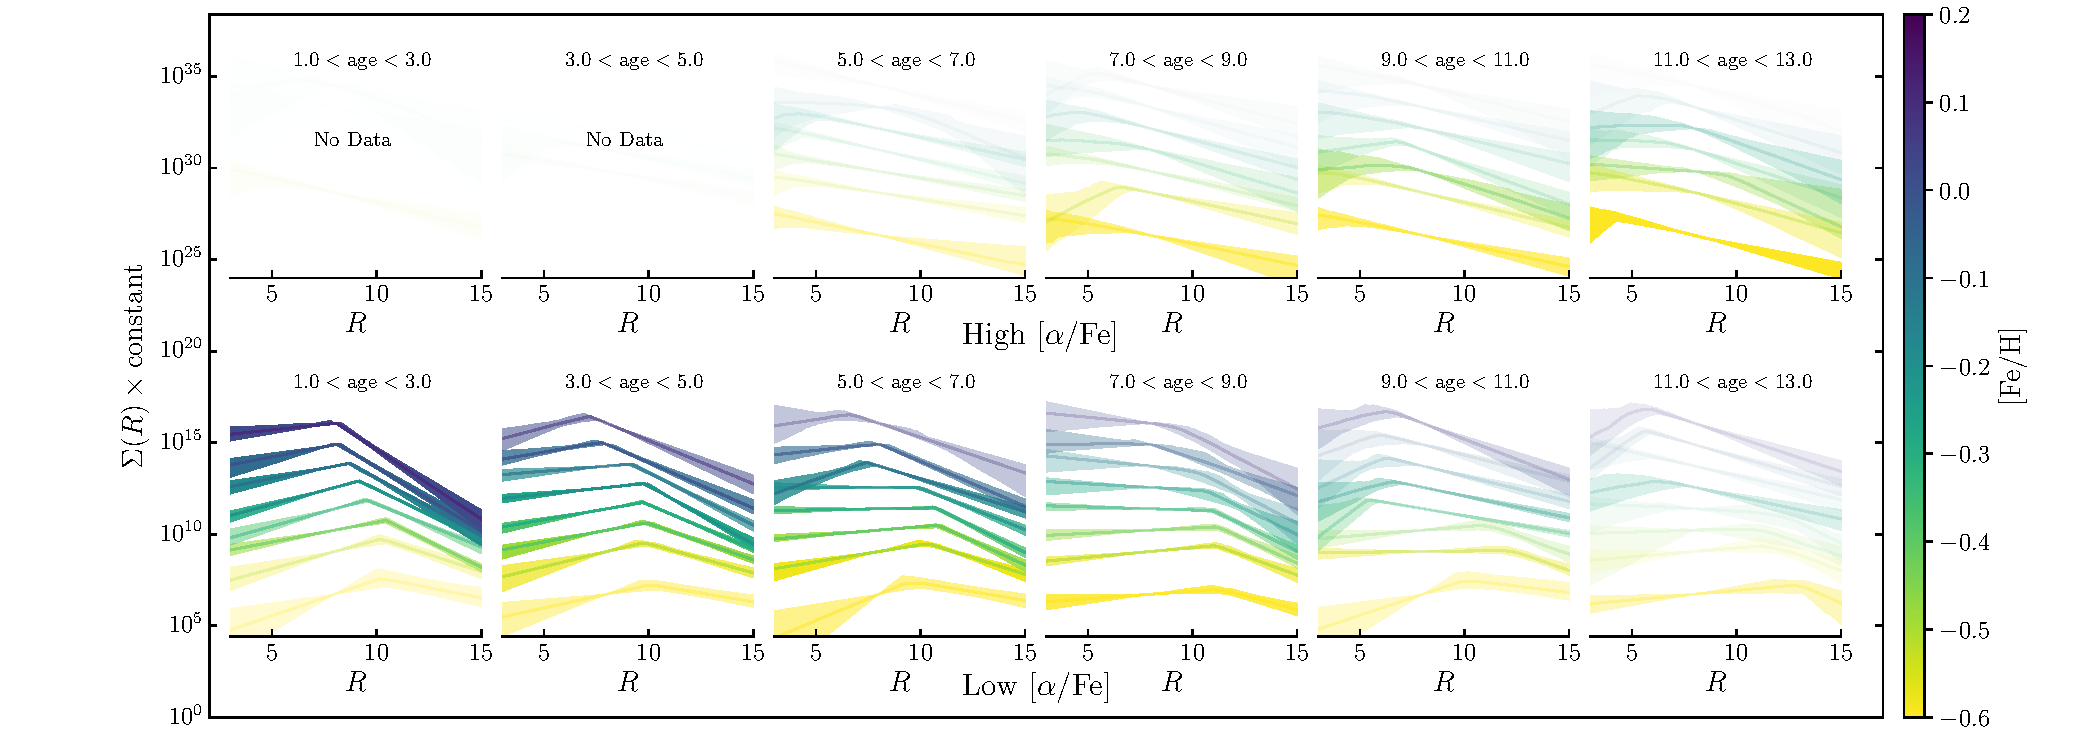
\includegraphics[width=1.0\textwidth]{surfdens_profile_adjusted.pdf}
      \centering
     \caption[Surface density profiles of mono-age, mono-\feh{} populations in the low and high-\afe{} disc components of the Milky Way]{The fitted surface density profiles for the high-\afe{} (\emph{top}) and low-\afe{} (\emph{bottom}) sub-samples as a function of \feh{} (colour) and age (increasing from left to right). The coloured bands represent the 95\% uncertainty range.  Only profiles for bins containing$ > 30$ stars are shown. The profiles have a transparency according to the surface-mass density calculated for each bin in Section \ref{sec:surfmassdens}, normalised separately for each row (i.e. in each \feh{} bin), to draw the eye to those profiles which contribute most to the Milky Way surface-mass density. High-\afe{} profiles are described well by a single exponential, whereas young, low-\afe{} profiles are broken exponentials with a peak density which varies in radius in the disc.}
     \label{fig:surfdens}
 \end{figure}
\end{landscape}


 \begin{figure}
 	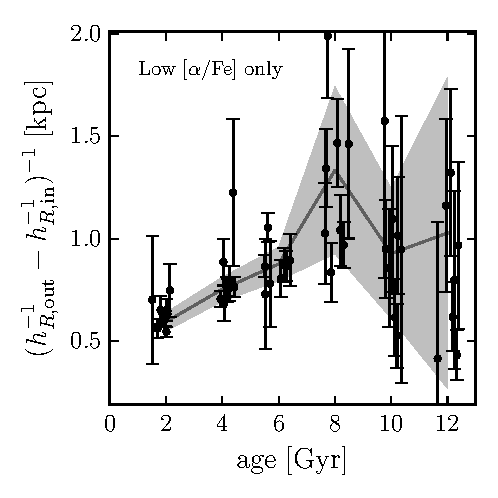
\includegraphics[width=0.6\columnwidth]{broadvsage.pdf}
     \caption[The broadening of surface density profiles as a function of age in the low-\afe{} mono-age, mono-\feh{} populations]{The profile width $(h_{R,\mathrm{out}}^{-1} - h_{R,\mathrm{in}}^{-1})^{-1}$ against age for the low-\afe{} populations (this diagnostic is irrelevant for the high-\afe{} populations, which are generally fit by single exponentials). A small random jitter is added to the central age of each age bin, to make individual points and their uncertainty clearer. The relations and coloured band shows the running surface-mass density weighted mean and standard deviation in the age bins. The profile width increases with age. A higher value of this diagnostic suggests a broader surface density profile, showing that older populations are flatter and broader around the peak density.}
     \label{fig:agevsbroadening}
 \end{figure}



\subsection{The vertical profile of the disc}
I now examine the variation of $h_Z$ as a function of radius in mono-age, mono-\feh{} populations. Because mono-age, mono-\feh{} populations are well described by a single scale height, which is modified by a flaring term $R_{\text{flare}}$, this means that $h_Z$ is weakly dependent on $R$ for profiles which flare. $h_Z$ as a function of $R$ for age-\feh{} bins with $> 30$ stars is shown in Figure \ref{fig:hzprofile}, adopting the same shading as Figure \ref{fig:surfdens} to draw the eye to the profiles with greater mass contribution. The dashed line represents $0.3$ kpc, for reference.

Figure \ref{fig:hzprofile} suggests that the disc is thicker as traced by older populations. All \feh{} bins thicken as age increases. This is clear in the left panel of Figure \ref{fig:agevshzrf}, which shows the surface-mass density weighted mean variation of $h_Z$ with age. The mean $h_Z$ spans the range between 0.2 and 0.8 kpc. The high-\afe{} populations have  a bump in the mean $h_Z$ at 8 Gyr, but $h_Z$ generally increases with age, similarly to the low-\afe{} populations. The shapes of the profiles of the youngest populations in Figure \ref{fig:hzprofile} in the low-\afe{} subsample show little variation with \feh{}, and this trend generally continues to older ages. This is also reflected in the low uncertainties associated with the blue points in the left panel of Figure \ref{fig:agevshzrf}. 


\begin{landscape}
 \begin{figure}
 	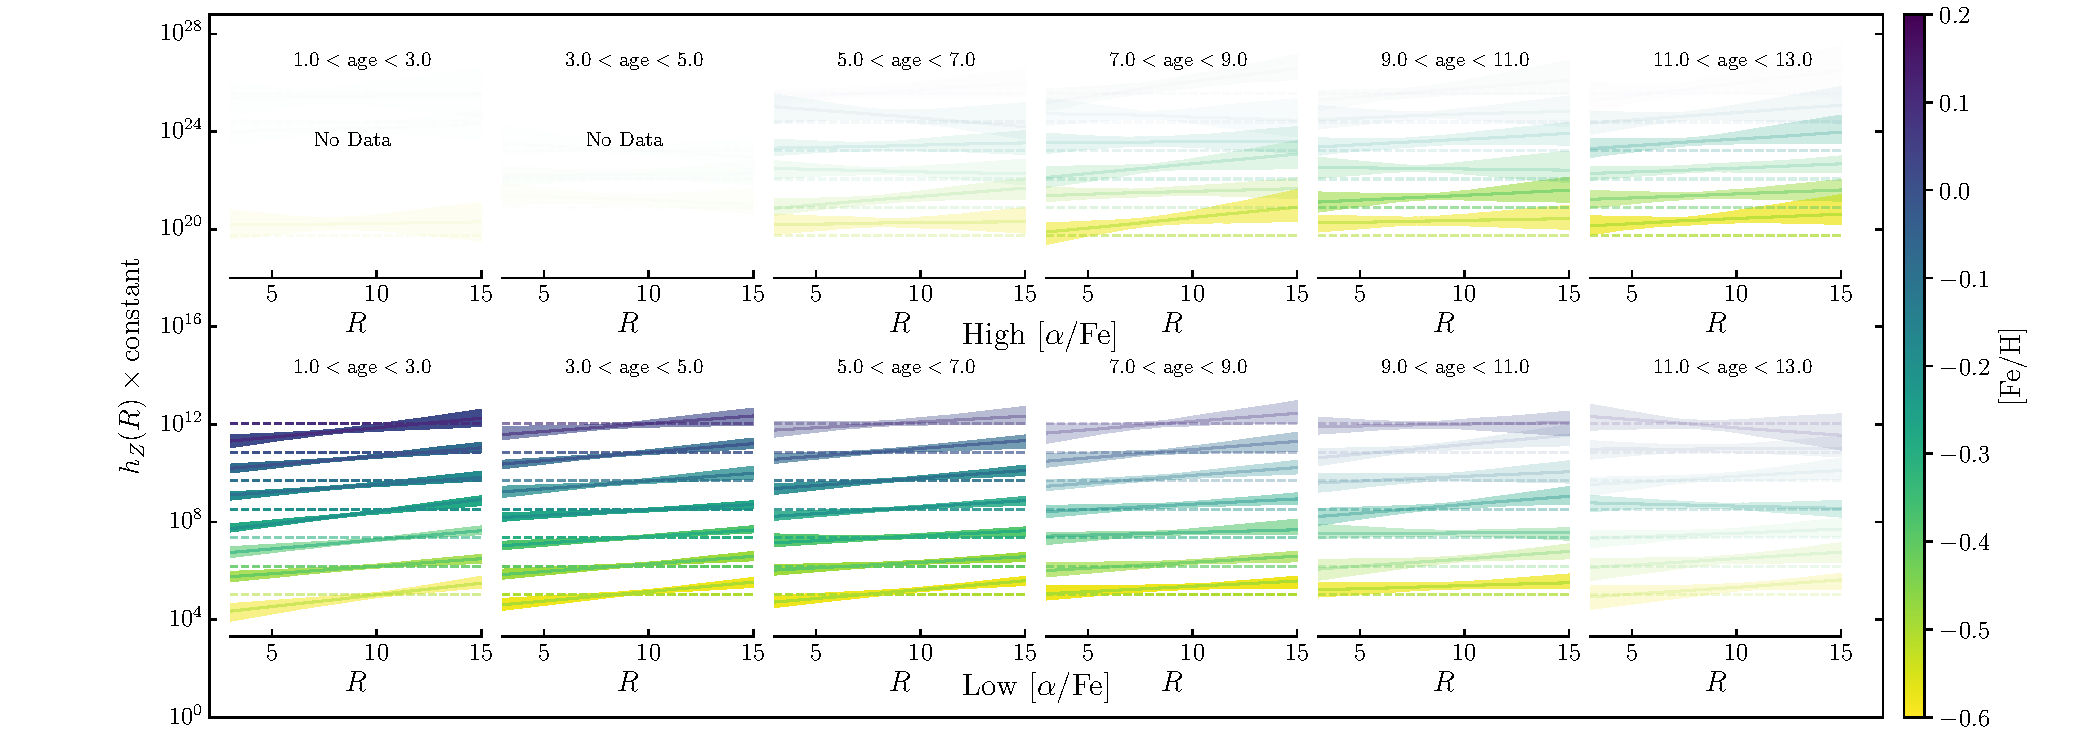
\includegraphics[width=1.\textwidth]{hz_profile_adjusted.pdf}
 	\centering
     \caption[Radial scale height profiles of mono-age, mono-\feh{} populations in the low and high-\afe{} disc components]{Vertical profiles for the high-\afe{} (\emph{top}) and low-\afe{} (\emph{bottom}) sub-samples as a function of \feh{} (colour) and age (increasing from left to right). The coloured bands represent the 95\% uncertainty range. Only profiles for bins with $> 30$ stars are shown, with profiles shaded according to their surface-mass density contributions (discussed in Section \ref{sec:surfmassdens}).  The dashed lines represent $h_Z = 0.3$ kpc, for reference.}
     \label{fig:hzprofile}
 \end{figure}
\end{landscape}


The high-\afe{} profiles are generally flat, indicating that these populations show little flaring. By multiplying together the PDFs of the posterior distributions of $R_{\mathrm{flare}}$ in each mono-age, mono\feh{} bin, I determine that the high-\afe{} populations have an average $R_{\mathrm{flare}}^{-1} = -0.06 \pm 0.02$. The low-\afe{} populations flare more strongly, with an average $R_{\mathrm{flare}}^{-1} = -0.12 \pm 0.01$. There is, however, some variation in the flaring as a function of age, so it may not be sensible to ascribe a single $R_{\mathrm{flare}}^{-1}$ to all the populations. The variation of $R_{\mathrm{flare}}^{-1}$ with age is shown in the right panel of Figure \ref{fig:agevshzrf}, which uses $R_{\mathrm{flare}}^{-1}$, rather than $R_{\mathrm{flare}}$, such that values very close to 0 are represented properly. The surface-mass density weighted mean $R_{\mathrm{flare}}^{-1}$ of the low-\afe{} populations increases as a function of age, meaning that the most flared populations are the youngest. The behaviour appears opposite for the high-\afe{} populations, whose mean $R_{\mathrm{flare}}^{-1}$ seems to decrease with age, but this is determined with low significance as $R_{\mathrm{flare}}^{-1}$ measurements are noisier for these populations.

\begin{figure}
	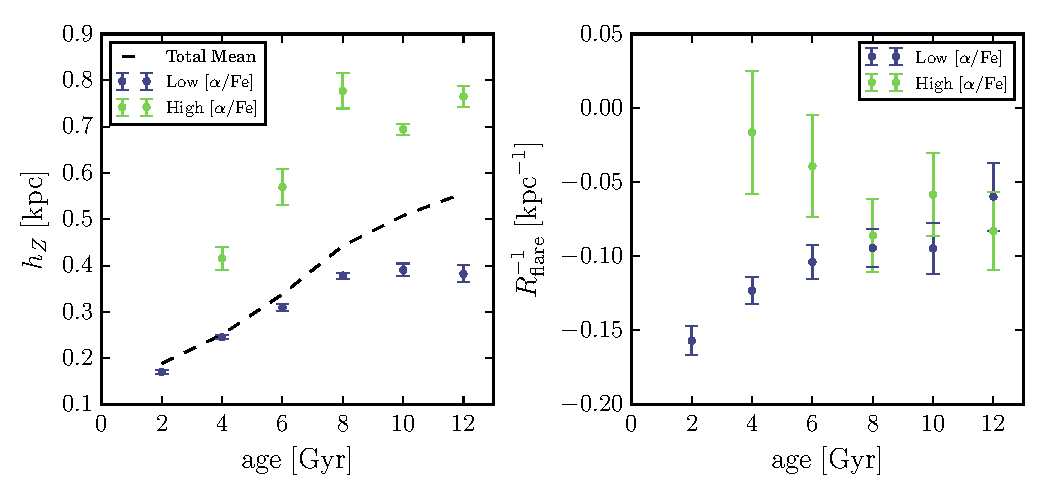
\includegraphics[width=\textwidth]{hzrfbroadvsage.pdf}
    \caption[$h_Z$ and $R_\mathrm{flare}^{-1}$ as a function of age for high and low-\afe{} mono-age populations in APOGEE DR12]{ Mean $h_Z$ at $R_0$ (\emph{left}) and $R_{\mathrm{flare}}^{-1}$ (\emph{right}) against age. The mean value in each age bin is calculated by multiplying together the posterior PDFs of the density fits. The panels show both the low (\emph{purple}) and high (\emph{green}) \afe{} populations. The left panel shows the total surface-mass density weighted mean as a dashed line, which demonstrates that the vertical distribution of the high-\afe{} population is only important at the solar radius at old ages due to its low surface-mass density contribution. $h_Z$ increases with age for both low and high-\afe{} populations. $R_{\mathrm{flare}}^{-1}$ behaves similarly for the low-\afe{} population, meaning flaring decreases with age, but the high-\afe{} population shows an opposite behaviour.}
     \label{fig:agevshzrf}
\end{figure}

\subsection{The mass contribution of mono-age, mono-\feh{} populations}
\label{sec:surfmassdens}
I now present the results from the calculation of the surface-mass density at the solar radius using the method described in Section \ref{sec:surfmasscalc}. The surface-mass density $\Sigma_{R_0}$ estimates are computed in each age-\feh{} bin in the high and low-\afe{} populations. When quoting the surface-mass densities, I also quote estimates of the systematic uncertainties. The sources of these uncertainties are evaluated and discussed in Section \ref{sec:discrepant}.

I combine the mass contributions of the high and low-\afe{} mono-age, mono-\feh{} populations, and plot these estimates as a function of age and \feh{} in Figure \ref{fig:margmass}. This Figure is representative of the \emph{mass-weighted} age-\feh{} distribution at the solar radius, i.e. it is equivalent to the probability distribution of age and \feh{} of a randomly selected mass element at the solar radius. The distribution varies smoothly with no sharp peaks, and the surface-mass density increases linearly with both age and \feh{}, peaking at $1 < \mathrm{age} < 3$ Gyr, $0.0 < \mathrm{[Fe/H]} < 0.1$ dex. The mass increases more smoothly with \feh{} than with age, but there is very little mass in the highest \feh{} bin, creating a ridge feature in the marginalised distribution. The distributions marginalised over age and \feh{} are clearly unimodal at this resolution, and there is little sign of any bimodality in age at fixed \feh{}. It should be mentioned again here that the age uncertainties may be larger than the bin width, particularly in older bins, which would cause an artificial blurring of a density edge in the distribution along the age axis. Therefore, one cannot presently determine to high significance that there are no discontinuities in this distribution.

\begin{figure}
 	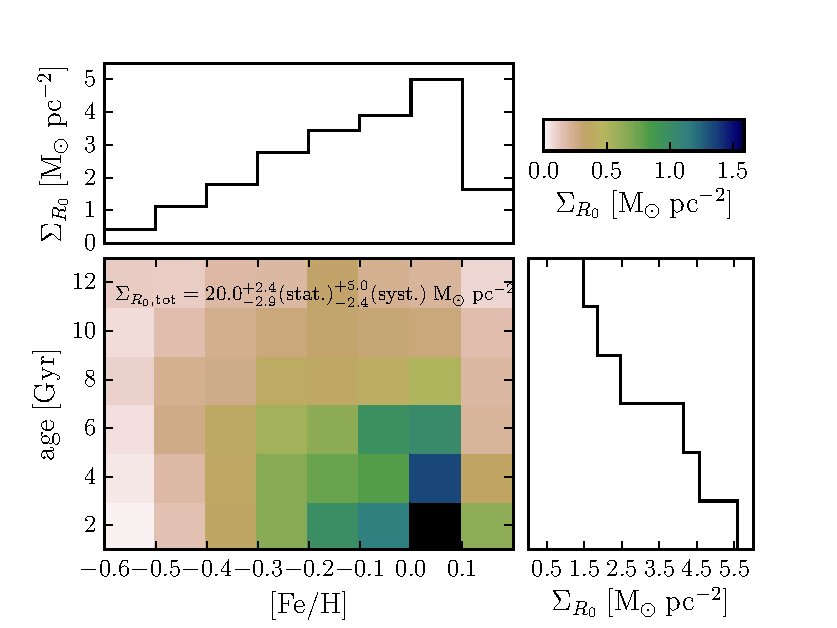
\includegraphics[width=\textwidth]{marginalised_colorblocks.pdf}
 	\centering
     \caption[The surface-mass density contribution of mono-age mono-\feh{} populations at the solar radius from APOGEE DR12]{The surface-mass density contribution of mono-age, mono-\feh{} populations at $R_0$ (where low and high-\afe{} are combined). The total contribution $\Sigma_{R_0,\ \mathrm{tot}}$ is displayed at the top of the main panel. The colour scale is linear and spans the surface-mass density range between $0 < \Sigma_{R_0} < 1.5\ \mathrm{M_{\odot}\ pc^{-2}}$. The marginalised distributions along each axis are shown above and to the right. The mass at the solar radius increases monotonically with both age and \feh{}. }
     \label{fig:margmass}
\end{figure}


An alternative way to look at the surface-mass density distributions is to retain the division in \afe{} used in the analysis. The high-\afe{} populations contribute $\Sigma_{R_0,\ \mathrm{tot}} = 3.0_{-0.5}^{+0.4}\mathrm{(stat.)}_{-0.6}^{+0.6}\mathrm{(syst.)}\ \mathrm{M_{\odot}\ pc^{-2}}$ to the total surface-mass density at the solar radius, whereas the low-\afe{} populations contribute $\Sigma_{R_0,\ \mathrm{tot}} = 17.1_{-2.4}^{+2.0}\mathrm{(stat.)}_{-1.9}^{+4.4}\mathrm{(syst.)}\ \mathrm{M_{\odot}\ pc^{-2}}$, giving a total surface-mass density in stars at $R_0$ of $\Sigma_{R_0,\ \mathrm{tot}} = 20.0_{-2.9}^{+2.4}\mathrm{(stat.)}_{-2.4}^{+5.0}\mathrm{(syst.)}\ \mathrm{M_{\odot}\ pc^{-2}}$. I plot the individual surface-mass contributions for the separated low and high-\afe{} populations in Figure \ref{fig:massafe}, adopting different color scales in each panel, to highlight the behaviour of the high-\afe{} populations, which contribute little mass in comparison to the low-\afe{}. The low-\afe{} mass is mostly concentrated at young age and towards higher \feh{}, although there is some mass even at the oldest ages. The high-\afe{} mass is concentrated towards older ages, but the distribution extends to high \feh{}, and mass is detected at some \feh{} in every age bin, albeit at much lower levels. The tails of the distributions of the low and high-\afe{} populations overlap somewhat in age-\feh{} space, around 6 Gyr ago, and there is a hint at the existence of a sequence extending from old, low \feh{} and high-\afe{} populations, to young, high \feh{} and low-\afe{} populations, which is somewhat visible in the combined histogram. There is no clear bimodality in age at fixed \feh{} in the combined histogram, owing to the very low mass contribution of the old, high-\afe{} populations. 

\begin{figure}
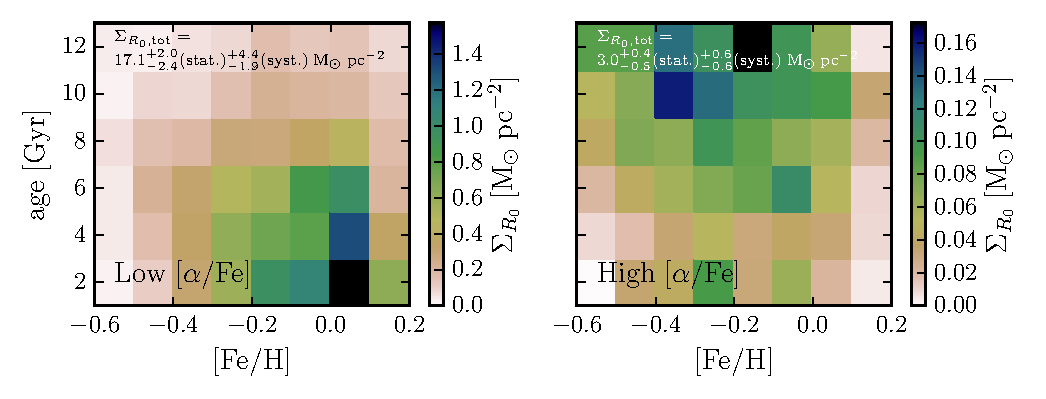
\includegraphics[width=\textwidth]{surfmassdensity_colourblocks_test.pdf}
 	\centering
     \caption[The separated surface mass density contributions of mono-age, mono-\feh{} populations in the low and high-\afe{} populations]{The surface-mass density contributions of the low (\emph{left}) and high (\emph{right}) \afe{} sub-samples. The total contributions $\Sigma_{R_0,\ \mathrm{tot}}$ are displayed at the top of each panel. I draw the attention of the reader to the difference in colour scale between the high and low-\afe{} panels, which differs by an order of magnitude, and is adopted to better show the behaviour in the high-\afe{} sample. The low-\afe{} sub-sample has mass at all ages and \feh{} but is concentrated mostly at young ages. The high-\afe{} sub-sample contributes far less mass and is concentrated at old age.}
     \label{fig:massafe}
\end{figure}


Thus far, I have established that the vertical spatial distributions of mono-age, mono-\feh{} populations are well described by single exponentials with a single characteristic $h_Z$. I now use this information to generate the mass-weighted distribution of $h_Z$, which is equivalent to the probability distribution function for $h_Z$, $p(h_Z)$. For a random stellar mass element, this function gives the probability density for the $h_Z$ of the component to which it belongs.  This relation is shown in Figure \ref{fig:hzhistogram}, where coloured points represent the individual density contributions of mono-age, mono-\feh{} populations, and the coloured histograms their co-addition within $\sim 0.1$ kpc wide bins in $h_Z$ for the low and high-\afe{} populations (purple and green, respectively). The dashed histogram represents the resulting total $p(h_Z)$. Scatter points are coloured by the age of the population they represent. The total distribution is smooth, resulting from the superposition of the low and high-\afe{} distributions, which overlap significantly.  The total $\Sigma_{R_0}$ (dashed histogram) declines exponentially with $h_Z$, and is unimodal with no gaps. The trends of both $h_Z$ and $\Sigma_{R_0}$ with age seen in Figures \ref{fig:agevshzrf} and \ref{fig:margmass} are recovered here, although it is surprising that the trend of $h_Z$ with age at the high $h_Z$ end does not appear as obvious here.

 \begin{figure}
	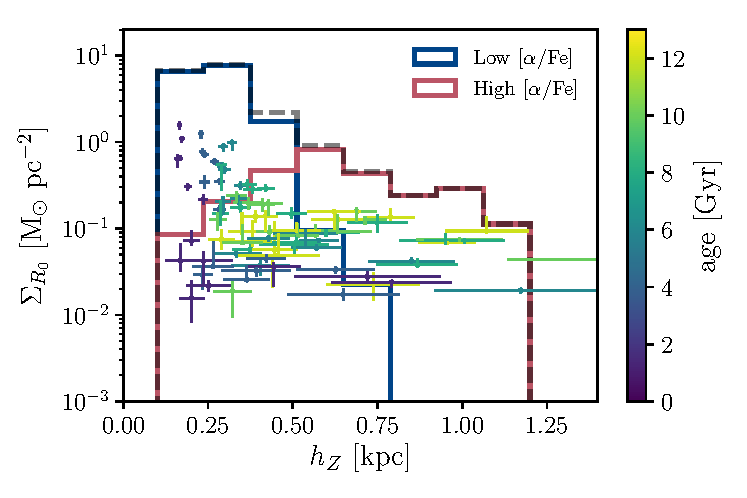
\includegraphics[width=\columnwidth]{thesis/Plots/adjusted_hz_sigma.pdf}
 	\centering
     \caption[The mass weighted vertical scale height distribution as calculated using mono-age, mono-\feh{} populations in APOGEE DR12]{The mass weighted vertical scale height $h_Z$ distribution. The individual points represent the $h_Z$ and $\Sigma_{R_0}$ for each mono-age, mono-\feh{} population. The points, which represent both the low and high-\afe{} populations, are coloured by the central age of the mono-age, mono-\feh{} bin that they represent. The coloured histograms represent the $h_Z$ distributions for the low and high-\afe{} populations from the sum of the individual contributions. The dashed histogram represents the total distribution. The total distribution smoothly decreases with $h_Z$, with no hints of bimodality.}
     \label{fig:hzhistogram}
 \end{figure}

I also now mass-weight and combine the fitted density profiles to attain the true surface-mass density profile of the Milky Way as a function of age, \feh{} and \afe{}. The resulting profiles are displayed in Figure \ref{fig:profcombo}. The different nature of the low and high-\afe{} populations in terms of spatial structure is clear here, with the low-\afe{} profile having a clear break between 8 and 10 kpc, and the high-\afe{} declining exponentially with $R$. It is interesting to note that extrapolation by eye of the high and low-\afe{} profiles to low $R$ would result in the high-\afe{} population becoming dominant over the low. The total profile appears roughly flat out to $\sim 10$ kpc. However, I \emph{strongly} emphasize that this is not determined to high significance, as even when only the uncertainties from the fitting procedure are included, one could describe the profile as exponentially declining with $R$ within $R < R_0$. The inclusion of the other sources of uncertainty on the surface-mass density estimates further decrease the significance of the apparent flattening. For example, the systematic uncertainties (discussed in Section \ref{sec:discrepant}) act to increase the fraction of surface-mass density contributed by the high-\afe{} populations, which would only \emph{increase} the slope of the inner exponential. Using dynamical tracers, \citet{2013ApJ...779..115B} find that the total surface density declines exponentially with R, so it seems logical to assume that the inner profile should not be increasing with R.

As a function of age, the peak in the surface-mass density visible in the youngest population becomes less prominent, and the profile becomes a roughly single exponential at the oldest ages (i.e., it monotonically decreases with $R$).  The behaviour with \feh{} is more complex, but the variation of the peak radius with \feh{} is obvious, and the turnover in the total profile at $\sim 10$ kpc appears to be a result of the outermost breaks.

\begin{figure}
 	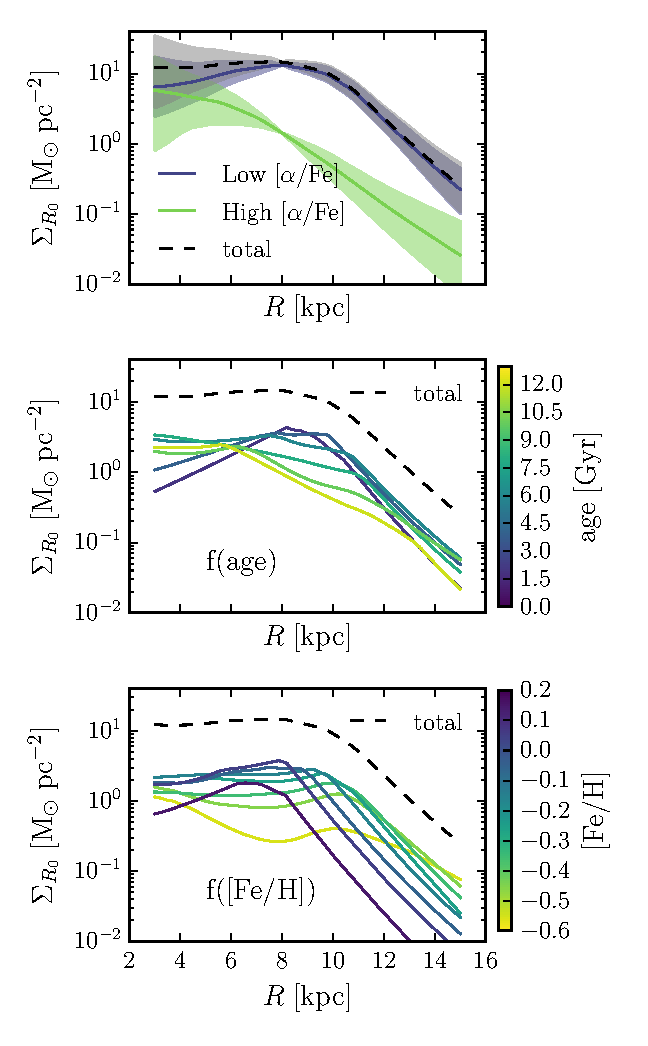
\includegraphics[width=0.7\columnwidth]{massweightedsurfdens.pdf}
 	\centering
     \caption[The best fit model for the true radial surface density profile of the Milky Way, as a function of age, \feh{} and \afe{} using mono-age mono-\feh{} populations in APOGEE DR12]{The radial surface-mass density profile of the Milky Way, as a function of \afe{} (\emph{top}), age (\emph{middle}) and \feh{} (\emph{bottom}). The profiles are the result of a mass-weighted combination of the fitted density profiles along different axes in age-\feh{} space and (in the top panel) for the combined low and high-\afe{} populations. Tthe combined uncertainties from the fitting procedure are shown in the top panel, which are sufficient (without addition of the individual statistical and systematic errors on the surface-mass densities, which are substantial) to show that the apparent flattening at $R < R_0$ is not found to high significance. The surface-mass density of low-\afe{} stars extends to a higher radius than the high-\afe{} stars. The youngest populations show a clearly peaked surface-mass density around the solar radius, whereas the older populations peak more centrally. Behaviour with \feh{} is complex, with flat profiles at low $R$, becoming exponentially decreasing at high $R$.}
    \label{fig:profcombo}
 \end{figure}

 \section{Discussion}
 \label{sec:discussiona}
 In the above analysis, I have, for the first time, determined the detailed structure of the Milky Way's disc as a function of stellar age and \feh{}. In our method, I have drawn heavily from previous dissections of the disc into its mono-abundance constituents \citep[MAPs;][]{2012ApJ...753..148B,2016ApJ...823...30B}, and so use these previous findings as a benchmark with which to compare these results. I will also show that our results are broadly consistent with other measurements, whilst shedding new light onto the problem of the formation of the Milky Way disc.


\subsection{Surface-mass density systematics}
\label{sec:discrepant}
I first address the sources of systematic uncertainty in our surface-mass density estimates, which are pertinent to the following discussions. The total local surface-mass density, including the correction for stars missing from the age catalogue, but before accounting for any other systematic uncertainties, is $\Sigma_{R_0, \text{tot}} = 20.0_{-2.9}^{+2.4}\ \mathrm{M_{\odot} \ pc^{-2}}$. This result is roughly two thirds as large as previous estimates, which are of the order $\Sigma_{R_0, \text{tot}} \sim 30\ \mathrm{M_{\odot} \ pc^{-2}}$ \citep[e.g.][]{2006MNRAS.372.1149F,2012ApJ...751..131B,2015ApJ...814...13M}. From canonical stellar evolution it is known that giants contribute very little to the total stellar mass in any population. For instance, \citet{2015ApJ...814...13M} find that giants make up $\sim 2\%$ of the local stellar mass. By virtue of this fact, conversions of the stellar mass inferred from giant-star counts to that of the total underlying stellar population require a multiplication of the observed counts by a factor of $\sim 50$, meaning that any uncertainty in the star counts is amplified in the final surface-mass density estimate. Our quoted statistical error estimates, however, which account for Poisson fluctuations in the stellar counts, cannot fully account for the discrepancy. 

I first evaluate whether such a discrepancy may be due to the assumed IMF or stellar evolution model. Tests adopting exponential \citet{2003PASP..115..763C} and \citet{2001MNRAS.322..231K} IMFs for the mass calculation resulted in variations of the final $\Sigma_{R_0, \text{tot}}$ estimate of the order $\sim 1\ \mathrm{M_{\odot}\ pc^{-2}}$, which I incorporate into the systematic error budget. I also re-ran the analysis on the basis of the BaSTI stellar evolution models \citep{2004ApJ...612..168P}, for which there also exists calculations for $\alpha$-enhanced stars \citep{2006ApJ...642..797P}. This test produces comparable estimates to the PARSEC models (after correcting for the fact that the lowest mass in the BaSTI isochrones is $0.5\  \mathrm{M_{\odot}}$ as opposed to $0.1\ \mathrm{M_{\odot}}$ in the PARSEC models). I also compute the mass using only APOGEE fields away from the plane (with $|b|\geq 6^{\circ}$), to test for the effects of extinction on the star counts, but attain results within the Poisson uncertainties of the original estimate.

I also apply our analysis procedure to a basic Monte Carlo mock sample, to check the method for converting observed counts to the real number density $N(R_0)$. I sample stars on a broken exponential density distribution with exponential flare then select points within APOGEE fields out to an imposed distance cut (which allows a simple reconstruction of the selection, and calculation of the effective volume). I then calculate $N(R_0)$ analytically, and also via our method, and find results which are consistent with the input parameters of the model, within the Poisson errors, for a wide variety of input parameters. 



As mentioned in Section \ref{sec:ages}, after making corrections to the ages, I find that the model returns ages greater than 13 Gyr for a sizeable number of stars \citep[][limit ages to 13 Gyr in their table]{2016MNRAS.456.3655M}. While these stars make up approximately $10\%$ of the final sample (3020 stars), they are not included in the number counts in each mono-age mono-\feh{} bin for calculation of the surface-mass density. Adding an extra $10\%$ of counts to each bin (in the same way as the extra $25\%$ is added in Section \ref{sec:ages}) introduces an extra systematic uncertainty of roughly $1\  \mathrm{M_{\odot}\ pc^{-2}}$ in each \afe{} sub-sample. However, readers should take into account that this simple correction does not account for a scenario where the stars with ages fitted $> 13$ Gyr might have a specific distribution in age, casting more counts in some bins (which might have more mass contribution per star) than others. For example, if these stars were all old, then the actual surface mass density in older bins would be higher than that found here, which would increase the total surface-mass density estimate. 

From the above, I robustly conclude that the majority of the systematic discrepancy is likely not due to the assumed IMF, stellar evolution model, dust extinction, or some peculiarity in the age measurements which affects star counts in the bins used. At this stage, it is difficult to understand what is the possible origin of this discrepancy with other works in the literature. Interestingly, this study is the only one employing giant stars as the stellar population tracer, which may point to possible systematics in the theoretical isochrones, or the APOGEE stellar parameters, or a combination thereof. It was demonstrated by \citet{2017A&A...597L...3M} that there may be significant issues with the spectroscopic determination of stellar surface gravity, which is dependent on the star's evolutionary state. I do find some discrepancy between the $\log{g}$ of the red clump between the PARSEC isochrones and the data, of the order $\sim 0.2$ to $0.3$ dex \citep[similar to that found by][albeit based on APOGEE-DR13 data]{2017A&A...597L...3M}, which could conceivably lead to problems in the conversion between star counts and mass. 

I test for the effect of systematics in the $\log{g}$ scale by shifting the $\log{g}$ cut of the isochrones to lower and higher $\log{g}$ by $0.3$ dex. I find that shifting the $\log{g}$ cut by $-0.3$ dex increases the surface-mass density estimate by $5.0\ \mathrm{M_{\odot}\ pc^{-2}}$. Increasing the $\log{g}$ cut by $0.3$ dex results in a decrease of $ 2.4\ \mathrm{M_{\odot}\ pc^{-2}}$. It therefore seems plausible that the discrepancy results from a systematic difference between the $\log{g}$ scales of the theoretical isochrones and APOGEE, and so I incorporate these shifts into the systematic error estimate. 

Upon inclusion of the systematic uncertainties from IMF variations and differences in the surface gravity scales, a final estimate of the total local surface-mass density in visible stars of $\Sigma_{R_0, \text{tot}} = 20.0_{-2.9}^{+2.4}\mathrm{(stat.)}_{-2.4}^{+5.0}\mathrm{(syst.)}\ \mathrm{M_{\odot} \ pc^{-2}}$, is attained from the addition of the low-\afe{} surface-mass density of $\Sigma_{R_0, \text{tot}} = 17.1_{-2.4}^{+2.0}\mathrm{(stat.)}_{-1.9}^{+4.4}\mathrm{(syst.)}\ \mathrm{M_{\odot} \ pc^{-2}}$, and the high-\afe{} value of $\Sigma_{R_0, \text{tot}} = 3.0_{-0.5}^{+0.4}\mathrm{(stat.)}_{-0.6}^{+0.6}\mathrm{(syst.)}\ \mathrm{M_{\odot} \ pc^{-2}}$.  If the $\log{g}$ systematics are as large as $-0.3$ dex, then this result is in agreement with the recent estimate from \citet{2015ApJ...814...13M}, of $27\pm 2.7\ \mathrm{M_{\odot} \ pc^{-2}}$.

A recent compilation of measurements of the thick and thin discs found that the thick-thin disc surface density ratio at $R_0$ is $f_{\Sigma} = 15\% \pm 6\%$ \citep{2016ARA&A..54..529B}. I find that $f_{\Sigma} = 18\% \pm 5\%$ for the high-low-\afe{} disc surface-mass density ratio, consistent with that estimate. While a better understanding of the possible systematics between the theoretical isochrones and APOGEE is beyond the scope of this paper, I have shown that even a slight difference in the $\log{g}$ scale can bring our results in line with existing estimates. This suggests that the surface-mass density measurement discrepancy here is indeed systematic, and that the high and low-\afe{} discs may still have some relation to the thick and thin components measured by these studies, which are mainly based on geometric decompositions of the disc. 

\subsection{Comparison with MAPs results}
\label{sec:bovycomparison}
I now discuss our density fits in comparison to the MAP measurements of \citet{2012ApJ...753..148B,2016ApJ...823...30B}. Such a comparison is important because this method is based on an extension of that developed by \citet{2016ApJ...823...30B} to the case of RGB stars, whose distances are far more uncertain than those of RC stars. \citet{2016ApJ...823...30B} used the APOGEE RC sample to find the structure of populations in narrow bins of \afe{} and \feh{}, which they term `mono-abundance populations' (MAPs). These MAPs represent stellar populations with a distribution of ages, but their interpretation assumes a significant relationship between age, \afe{} and \feh{}. I can now compare results when the third parameter, age, is known.  

\citet{2016ApJ...823...30B} showed that the radial distribution of low-\afe{} MAPs is well described by a broken exponential, and I confirm this result, showing that each of the low-\afe{}, mono-age, mono-metallicity populations is also described by a radially broken exponential. I also show that the older, high-\afe{} populations are instead described by a single exponential, which is in good agreement with the findings of \citet{2016ApJ...823...30B}.

The dependence of the radial distribution of mono-\feh{} populations on age is interesting in this regard.  The low-\afe{} population, for which our sample covers a wide range of ages with high signal-to-noise, shows a broadening of the profile around a density peak towards older populations, at all \feh{}. This effect does not appear to be present in the high-\afe{} population (although some populations have slight evidence of a break at low significance), which suggests that it was formed and evolved differently. The implications of these findings are more fully discussed in Section \ref{sec:implications}.

I also confirm the results of \citet{2016ApJ...823...30B} which showed that the break radius, $R_{\mathrm{peak}}$ is a declining function of \feh{}. I show that, in the low-\afe{} population, at fixed age, $R_{\mathrm{peak}}$ moves to smaller radii as \feh{} increases. As a function of age, the amplitude of this variation increases. The difference in $R_{\mathrm{peak}}$ at the highest and lowest \feh{} in the 6 Gyr bin is $\sim 6$ kpc, which is identical with that of the profiles shown in Figure 11 of \citet{2016ApJ...823...30B}.
 
\citet{2016ApJ...823...30B} found that low-\afe{} MAPs were fit well with a $h_Z(R)$ which was slowly exponentially flaring with $R_{\mathrm{flare}}^{-1} = -0.12 \pm 0.01 \ \mathrm{kpc^{-1}}$. I also confirm this result, finding that low-\afe{} populations have, on average, $R_{\mathrm{flare}}^{-1} = -0.12 \pm 0.01 \ \mathrm{kpc^{-1}}$. However, I also find that $R_{\mathrm{flare}}^{-1}$ shows considerable variation with age (around this mean) in the low-\afe{} populations. While \citet{2016ApJ...823...30B} found that high-\afe{} populations were consistent with a having $R_{\mathrm{flare}}^{-1} = 0.0 \pm 0.02\ \mathrm{kpc^{-1}}$, I find that these populations have $R_{\mathrm{flare}}^{-1} = -0.06 \pm 0.02\ \mathrm{kpc^{-1}}$, showing some evidence of flaring, albeit at a lower level and lower significance than the low-\afe{} populations.

 It was also shown by \citet{2012ApJ...753..148B,2016ApJ...823...30B} that the $h_Z$(\afe{},\feh{}) of MAPs smoothly spans the range between 0.2 and 1 kpc. I confirm and extend this result, showing that $h_Z$(age,\afe{},\feh{}) varies smoothly between a maximum $h_Z$ of $\sim 1.2$ kpc in the high-\afe{}, low \feh{}, older populations, down to a minimum of $\sim 0.2$ kpc in the youngest, low-\afe{}, \feh{} rich populations. Figure \ref{fig:hzhistogram} can also be directly compared with Figure 2 of \citet{2012ApJ...751..131B}, which showed that the mass-weighted $h_Z$ distribution is not bimodal but smoothly declines with $h_Z$. I confirm that result, showing that for mono-age, mono-metallicity populations, the mass weighted $h_Z$ distribution shows no sign of bimodality; The low and high-\afe{} population $h_Z$ distributions are distinct but overlap significantly, generating a smooth distribution. This presents an interesting new look at the interplay between spatial and chemical structure in the disc, as there is a clear mixing spatially of the two chemically separated populations. The implications of this finding are intriguing, and I discuss them further in Section \ref{sec:implications}.

\citet{2012ApJ...751..131B} also made a measurement of the local surface-mass density, finding (in the original application of the method used here) that SEGUE G-type dwarfs yield an estimate of $\Sigma_{R_0,\text{tot}} = 30 \pm 1\ \mathrm{M_{\odot}\ pc^{-2}}$, which is in good agreement with other studies based on different samples \citep[e.g.][]{2006MNRAS.372.1149F,2015ApJ...814...13M}.  Comparatively, the estimate based on APOGEE DR12 somewhat smaller, even when systematics are taken into account. There are a number of differences between this study and that of \citet{2012ApJ...751..131B}. For example, the increased radial coverage, adoption of RGB stars as a tracer, and the fits based on mono-age, mono-metallicity (rather than mono-abundance) populations. However, as mentioned above in Section \ref{sec:discrepant}, these results, after accounting for systematic uncertainties, appear in good agreement with other, more recent estimates \citep{2015ApJ...814...13M}. 

\subsection{Comparison with other Milky Way disc studies}
I now make qualitative comparisons of the findings of this analysis with the broader body of knowledge regarding the Milky Way disc structure \citep[see, e.g.][for recent reviews]{2013A&ARv..21...61R,2016ARA&A..54..529B}. In comparing these results with those from previous studies, I am constrained to making mostly qualitative considerations, as previous work is based on fits of single exponential profiles to the radial component of the stellar density distribution.

This work strongly constrains the structure of both the low and high-\afe{} components in the Galactic disc, which are commonly considered to be interchangeable with the thin and thick components \citep[as asserted by, e.g.][]{2004A&A...415..155B,2012A&A...545A..32A,1998A&A...338..161F}. I have shown that the \afe{} rich component, while corresponding to a thicker configuration in general, is the product of individual mono-age populations of varying thickness. I also find that the \afe{} rich populations span the range  $ 0.4 < h_Z < 1$ kpc, with $h_Z$ increasing with age. Studies of the vertical disc structure which fit a double exponential find a thick disc scale height of $\sim 1$ kpc  \citep[e.g.][]{1983MNRAS.202.1025G,2008ApJ...673..864J}, which is fully consistent with measurements of the thickest high-\afe{}, old, mono-age populations in our analysis. However, I again stress here that the age uncertainties at old ages may be significantly larger than the bin size, which may cause a blurring of these trends, and should be accounted for when comparing these results to models. As an example, in the \emph{worst case} scenario, assuming gaussian errors, the oldest bins (between 7 and 13 Gyr) may be contaminated by up to $50\%$ of the stars which should be assigned to neighbouring bins, at the oldest end, with the fraction dropping off quickly at younger ages. I briefly discuss the implications of the worst case blurring on our interpretation of these trends in Appendix \ref{sec:ageerror}.

Regarding the radial scale length of the thick component, I find an obvious discrepancy with literature values, whereby our thick, high-\afe{}, populations have an average $h_{R, \text{out}} = 1.9 \pm 0.1  $ kpc, while the aforementioned studies, who define the thick disc geometrically, find values of the order $\sim 4$ kpc \citep{2001MNRAS.322..426O,2008ApJ...673..864J}. This discrepancy appears to arise in the choice of definition of the measured population between a geometric or chemical abundance selection, with many studies finding a scale length for the abundance-selected $\alpha$-rich disc in the range $h_R = 2.0 \pm 0.2$ kpc \citep{2016ARA&A..54..529B,2016ApJ...823...30B,2012ApJ...753..148B,2012ApJ...752...51C}. It should be noted here that the $h_{R, \text{out}}$ found here would likely be in even better agreement with this value, had the 5\% systematic discrepancy in the distances (shown in Figure \ref{fig:distcomp}) been accounted for. \citet{2016arXiv160901168M} recently showed evidence for a radial age gradient in the Milky Way, suggesting this as a source of disagreement between abundance-selected and geometric studies of the thick disc components, where the geometric selected studies see an extended thick disc which is made up of flared low-\afe{} populations. 

I also re-examine claims of a sharp decline in the stellar density at $R\sim 13.5$ kpc \citep[e.g.][]{2009A&A...495..819R,2010MNRAS.402..713S} in light of these results. \citet{2010MNRAS.402..713S} fit a single exponential density profile with scale-length $\sim 3$ kpc to A stars (which preferentially selects stars younger than $\sim 100$ Myr old) and found that after $R\sim13$ kpc, a model with shorter scale-length was necessary to explain the increased rate of decline in stellar density. The total profile in Figure \ref{fig:profcombo} begins to decline after $R\sim10$ kpc. The uncertainties in the measurement of the mass contribution of each profile may cause some discrepancy here, as implying a higher mass on older or more metal poor populations would shift this turn-over to higher radii. I also fit older populations than \citet{2010MNRAS.402..713S}, which, under the inside-out formation paradigm, might suggest another reason for such a discrepancy, as older populations would be more centrally concentrated. I confirm the assertion of \citet{2016ApJ...823...30B} that this break, clearly visible in the total stellar distribution, is attributable to the outermost break of the mono-\feh{} profiles - which are shown in the bottom panel of Figure \ref{fig:profcombo}. External disc galaxies are also observed to have such a truncation in their stellar density profiles \citep[e.g.][]{2006A&A...454..759P}. 


\subsection{Implications for the formation of the Galactic disc}
\label{sec:implications}

In light of the above discussion, I now present the implications of these results for the formation of the Galactic disc. In this chapter, I present a detailed dissection of the disc by age, \feh{}, and \afe{}, and as such, present a previously unseen picture of the dominant structure of the Milky Way. In studying mono-age populations, I enable a more direct comparison than previously possible with numerical simulations of Milky Way type galaxies, which tend to use age information in the absence of detailed chemical modelling.

\subsubsection{Disc flaring, profile broadening and radial migration}

By estimating the density profiles of mono-age populations, I  place novel constraints on radial migration and its effects on the structure and evolution of the disc. I describe two key observables which provide this insight: the flaring of the disc, which has been considered as an effect of vertical action conserving radial migration \citep[where stars have greater vertical excursions as they migrate outward, e.g.][]{2012A&A...548A.127M}, and the broadening of the density profiles around the peak with time, which I discuss as a potential new indicator of radial migration. The right panel of Figure \ref{fig:agevshzrf} shows a clear trend of increasing $R_{\mathrm{flare}}^{-1}$ with age such that the youngest populations flare most. This behaviour is distinct from the results of \citet{2016ApJ...823...30B}, which found that low-\afe{} populations were described by a single $R_{\mathrm{flare}}^{-1}$. It is, however, conceivable that if low-\afe{} populations of all ages are combined, the resulting population may have a similar behaviour to that in \citet{2016ApJ...823...30B}. Indeed, I find an average $R_{\mathrm{flare}}^{-1} = -0.12\pm 0.01\ \mathrm{kpc^{-1}}$, which is in good agreement with the value from \citet{2016ApJ...823...30B}. If populations become more flared as radial migration proceeds, then it becomes difficult to reconcile our result with that of a disc whose stars continually underwent radial migration, largely unperturbed by any mergers that might cause structural discontinuity \citep[e.g.][]{2014MNRAS.442.2474M}, especially under suggestions that mergers actually reduce flaring from radial migration \citep[e.g.][]{2014A&A...572A..92M}. In this context, this result is indicative of an old population in the Milky Way which has undergone some mergers, reducing the flaring in the oldest populations. It should be noted here, however, that the age uncertainties (which can be as large as $40\%$) could effectively artificially increase the age bin size, super-imposing populations with different scale heights and flare, and reducing the overall flaring profile.

I show in Figures \ref{fig:agevsbroadening} and \ref{fig:surfdens}  that the radial surface density profiles of low-\afe{} populations become smoother with age. Interestingly, the position of the break radius does not vary monotonically with age. Assuming that the peak radius is at the equilibrium point of chemical evolution for a given population  \citep[where the consumption of gas and its dilution are balanced, as discussed in][]{2016ApJ...823...30B}, then one might consider that such a broadening would occur if stars that formed near the equilibrium point migrated inwards and outwards over time.  If these assumptions are correct, then the specific surface density profile shapes might provide insights into how radial migration has proceeded in the disc. For example, if the slope of the inner or outer profile change slope differently, this might suggest that migration has been asymmetric (i.e. more mass has moved in than out or vice versa). Comparing the $-0.2 <\mathrm{[Fe/H]}<-0.1$ dex and $0.0 <\mathrm{[Fe/H]}<0.1$ dex bins in Figure \ref{fig:surfdens}, it seems that the \emph{inner} slope of the former profile decreases more with age, whereas the \emph{outer} slope of the latter decreases more strongly, suggesting that the former population has preferentially migrated in, whereas the latter migrated out.  It is important to point out that under the interpretation that the increasing profile width is due to migration efficiency, I make an assumption that stars of a given \feh{} and \afe{} must have been born with the same profile width throughout cosmic time \citep[as discussed by, e.g.][]{2017ApJ...834...27M}.


This picture is also consistent with the suggestion by, e.g, \citet[][]{2015ApJ...808..132H,2011ApJ...737....8L}, that the changing skew in the MDF as a function of Galactocentric radius is caused by such a mechanism. In Figure \ref{fig:mdf}, I show the mass-weighted \feh{} distribution for the low-\afe{} fits at different Galactocentric radii, showing that these results both find a radial metallicity gradient, and qualitatively reproduce the skew found by \citet[][]{2015ApJ...808..132H}. Unlike \citet[][]{2015ApJ...808..132H}, this analysis fully corrects for sample-selection and stellar-population biases in reconstructing the MDF. \citet{2016MNRAS.460L..94G} also found similar behaviour in a simulated galaxy, finding that spiral structure induces different migration patterns, dependent on birth radius. 

\begin{figure}
	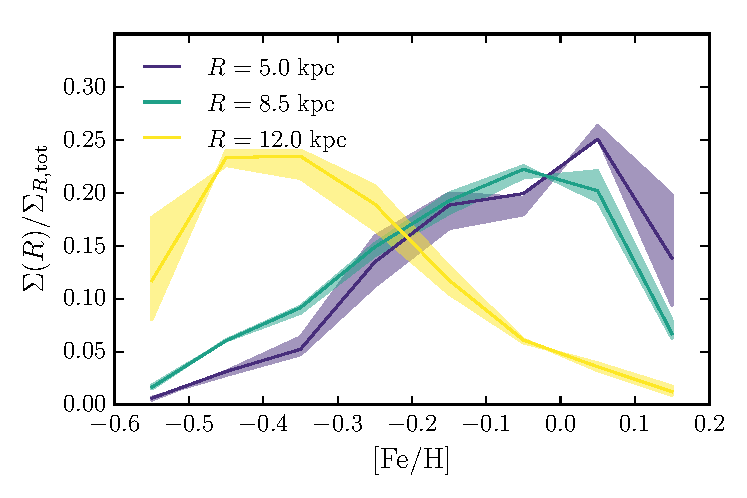
\includegraphics[width=0.8\columnwidth]{MDFs_radii.pdf}
 	\centering
   \caption[Surface-mass denisty weighted \feh{} distribution in 3 radial bins, as found from measurement of mono-age, mono-\feh{} populations in APOGEE DR12]{The surface-mass density weighted \feh{} distribution (MDF) at 3 radii for profiles fit to the low-\afe{} populations. The distribution shown is marginalised in age across all age bins. The coloured bands give the 95\% uncertainty ranges, where uncertainties are dominated by those on the fitted density profiles. The mean \feh{} is lower at greater $R$. Qualitatively, the skew of the MDF's changes with $R$, such that the innermost $R$ has a tail going to low \feh{}, and the outermost $R$ has a tail going to high \feh{}}
     \label{fig:mdf}
 \end{figure}

Interestingly, I detect the possible flaring of old, high-\afe{} populations, with average $R_{\mathrm{flare}}^{-1} = -0.06 \pm 0.02\ \mathrm{kpc^{-1}}$. However, the right panel of Figure \ref{fig:agevshzrf} shows that the flaring of the high-\afe{} populations does not vary as strongly with age as the low-\afe{} populations (although it should be noted that most of the mass in the high-\afe{} populations is concentrated at older age anyway). The detection of even a slight flare in these populations is surprising, as \citet{2016ApJ...823...30B} found that the high-\afe{} MAPs did not have any flare. Again, this may be an effect of the superposition of multiple mono-age populations within the MAPs. For example, \citet{2015ApJ...804L...9M} found that co-eval populations in simulated galaxies always flare, and suggested that the superposition of such flares might be an explanation for thickened disc components. \citet{2017ApJ...834...27M} showed that the superposition of mono-age populations within MAPs can introduce decreased flaring in high-\afe{} populations, whilst the mono-age populations themselves still flare. Comparison of these results with \citet{2016ApJ...823...30B} seems to present a consistent scenario. It should be noted here however, that \citet{2013MNRAS.436..625S} found that MAPs in their simulation were coeval in general.

These results show that the oldest populations are thicker, centrally concentrated, and display the least flaring, whilst the youngest populations, which show the most flaring, have the thinnest vertical distribution (smallest $h_Z$). Between these extremes, consecutive populations in age form a continuum, when the combined low and high-\afe{} structure is considered (see Figure \ref{fig:agevshzrf}). It is clearly conceivable then, that the \emph{geometrically} defined thick disc, found to have large scale-length \citep[e.g.,][]{2013MNRAS.431..930J,2008ApJ...673..864J}, may be the superposition of these flared (young) and naturally thick (old) components. An obvious consequence of this scenario would be an age-gradient at high $Z$ above the disc plane, which has been recently shown to be present in the APOGEE data by \citet{2016arXiv160901168M}. It was also recently shown that the mean structural characteristics of the abundance selected thick and thin discs appear to overlap at $\mathrm{[M/H]}\sim-0.25$ dex and \afe{} $\sim 0.1$ dex in the Gaia-ESO dataset \citep{2014A&A...567A...5R}, further presenting a scenario where the thick and thin disc components are not necessarily separable from one another, or at least not in abundance space. 

\subsubsection{Inside out formation, and the overall vertical disc structure}
The formation of the Galactic disc is commonly framed in the paradigm of inside-out formation \citep[e.g.,][]{2013ApJ...773...43B,2011ApJ...729...16K,1976MNRAS.176...31L,1989MNRAS.239..885M}. More recently, the effects of radial migration  \citep[e.g.][]{2002MNRAS.336..785S} were added, in order to produce models that agree better with the observations \citep[e.g.][]{2011ApJ...737....8L,2009MNRAS.396..203S,2015ApJ...802..129S,2015A&A...580A.126K} . The measurements of the peak radius of mono-age populations  presented in this chapter place strong empirical constraints on the evolution of the Milky Way disc over time. The behaviour of $R_{\mathrm{peak}}$ with age and \feh{} is shown in Figure \ref{fig:rpeakvsage}. I find that the surface-mass density weighted mean $R_{\mathrm{peak}}$ of low-\afe{} populations remains roughly constant with age, whilst the dispersion about the mean increases with age. This finding is qualitatively consistent with that of e.g. \citet{2016arXiv160804951A}, who show that the radial metallicity gradient decreases with the age of the population considered. These results show that the density peaks of mono-\feh{} populations become more separated with age. As the mean \feh{} at a given $R$ is dictated by the dominant population in stellar density at that radius, this indicates that these results also find a shallowing gradient in \feh{} with age. This is reinforced by our finding (also shown in Figure \ref{fig:rpeakvsage}) that the mean $R_{\mathrm{peak}}$ decreases with \feh{}.

\begin{figure}
	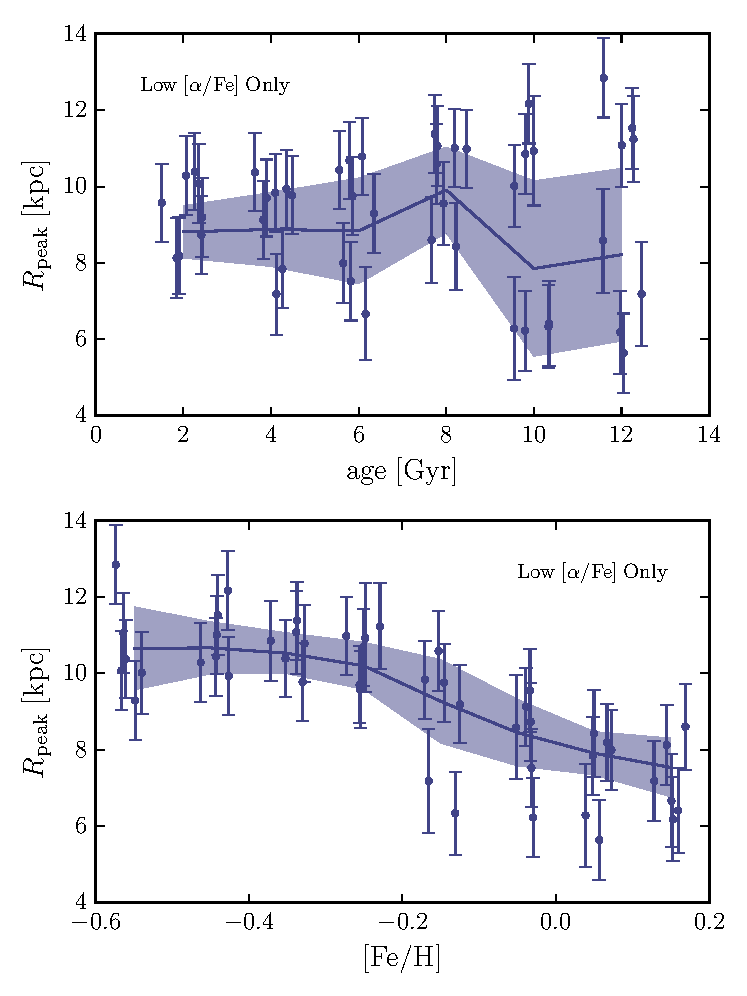
\includegraphics[width=0.8\columnwidth]{rpeakvsage.pdf}
	\centering
   \caption[Peak radius of surface density profiles in the low-\afe{} mono-age, mono-\feh{} populations in APOGEE DR12, shown as a function of age and \feh{}]{The behaviour of $R_{\mathrm{peak}}$ with age and \feh{} for the low-\afe{} populations. The high-\afe{} populations are better fit by single exponentials, and so $R_{\mathrm{peak}}$ is not an informative diagnostic of these populations. The coloured lines and bands give the surface-mass density weighted mean and standard deviation within an age or \feh{} bin. The mean $R_{\mathrm{peak}}$ does not vary significantly with age, whereas it shows a clear decrease with \feh{}. However, the dispersion in $R_{\mathrm{peak}}$ does increase with age for low-\afe{} populations. high-\afe{} populations show a slight increasing trend for increasing age and \feh{}, albeit at low significance. }
    \label{fig:rpeakvsage}
 \end{figure}


These results also place strong constraints on models for the formation of the vertical disc structure. I have already discussed that the vertical structure of the disc is commonly framed as having two geometrically distinct (but overlapping) vertical components \citep[e.g.][]{1983MNRAS.202.1025G}. The results of this chapter confirm previous work \citep[e.g.][]{2012ApJ...751..131B} which shows that this picture, while providing an acceptable description of the data when analysing the whole population, is not complete when individual populations, either abundance- or age-selected, are considered. I have shown (in Figure \ref{fig:hzhistogram}) that for a random mass element, the probability that it belongs to a population of a given $h_Z$ exponentially declines as $h_Z$ increases. There are no apparent breaks in this relation at the resolution which it is measured here, strongly suggesting that the spatial vertical disc structure is continuous. This finding, in stark contrast to the distinct discontinuities seen in the chemical structure of the entire disc \citep[e.g][]{2014ApJ...796...38N,2015ApJ...808..132H}, presents an interesting conundrum for galaxy formation theory. How is it possible that the \emph{spatial} structure of the disc be smooth and continuous, whilst the \emph{chemical} structure portrays a clear discontinuity?

Theoretical studies have, thus far, presented some clues as to how galaxy discs such as that of the Milky Way might form. As most studies fit single exponential radial profiles to simulated discs, quantitative comparisons are difficult, yet qualitative considerations can be made. \citet{2013MNRAS.436..625S} used a maximum likelihood method similar to \citet{2012ApJ...753..148B} to fit density profiles to MAPs in a simulated galaxy and found a continuous distribution of scale heights, but also found that their simulation showed a strongly geometrically distinct thick disc component. \citet{2013ApJ...773...43B} made detailed measurements of the mono-age populations in a high-resolution hydrodynamic Milky Way-like galaxy simulation, and found, similarly to these results that their scale heights gradually decreased with time, while the scale lengths increased, with populations forming thick and retaining that thickness in an 'upside-down and inside-out' disc formation. These results also find evidence of flaring in the thick components (as discussed in Section \ref{sec:bovycomparison}), which may point towards some structural evolution (via a process such as radial migration) after their formation. However, work on simulations by \citet{2009ApJ...707L...1B}  suggests early, turbulent gas as the origin for thicker disc components. A flare in the gas disc of the Milky Way, associated with the stellar component, is also observed in numerous studies \citep[e.g.][]{2014Natur.509..342F,2014ApJ...794...90K,1963SvA.....6..658L}, suggesting a formation of the disc with structural parameters similar to its progenitor gas disc.
 
\subsubsection{The age-\feh{} distribution and the evolution of the disc}
I now discuss how the present day structural parameters, in combination with the emergent picture of the mass distribution in age-\feh{} space at the solar radius, might offer deeper insights into the formation and evolution of the disc. 

I find, as may be expected, that the high-\afe{} populations contribute the majority of their mass at the solar radius at ages older than $\sim 6$ Gyr, although the mass contribution by old stars is extremely low compared to the younger populations. The middle panel of Figure \ref{fig:profcombo} shows that, if the populations follow the density models that I have fit, then the older stars become more dominant closer to the Galactic centre, which is suggestive of a weak mean radial age gradient, in qualitative agreement with theoretical predictions \citep[e.g.][]{2015ApJ...804L...9M} and observations of the thick disc \citep[e.g.][]{2016arXiv160901168M}. It is therefore not surprising that the bottom panel of Figure \ref{fig:profcombo} shows a clear variation in mean metallicity, in agreement with findings in other works \citep[e.g.][]{2012ApJ...746..149C,2016arXiv160804951A,2015ApJ...808..132H}. Only with high resolution hydrodynamical simulations, which accurately reproduce the stellar populations in galaxies, will it be possible to reconstruct the right combination of star formation history and radial mixing that led to these age and metallicity gradients, to gain a better understanding of the details of their formation.

In Figure \ref{fig:massafe}, an overlap in age-\feh{} space is visible between the high and low-\afe{} populations. While there appears to be mass at many \feh{} bins in the old populations, the overlap in age occurs at intermediate \feh{} at the solar radius. Previous studies have found that the youngest stars in the high-\afe{} sequence overlap in age with the oldest and most \feh{} poor stars in the low-\afe{} population \citep[e.g.][]{2013A&A...560A.109H}, and these findings appear to be consistent with that result. It should however, be noted, that at least some of this overlap is likely caused by the age uncertainties, which can be as high as 40\%. If the low-\afe{} population emerged from the remnants of the high-\afe{}, then it is likely that some sort of infall event must have occurred to return the ISM to low \feh{} and low-\afe{} before forming those stars \citep[as expressed by, e.g.,][]{1997ApJ...477..765C}. These scenarios are also discussed in the context of the APOGEE results by \citet{2014ApJ...796...38N}. To fully understand this, however, we will likely require a chemodynamical model which reproduces the bimodality in \afe{} at fixed \feh{}.

\section{Conclusions}
\label{sec:conclusionsa}

I have performed the first detailed dissection of the stellar populations of the Milky Way disc in age, \feh{} and \afe{} space, bridging the gap between the detailed observational understanding of mono-abundance populations \citep[e.g.][]{2012ApJ...753..148B,2016ApJ...823...30B} and the plethora of studies of co-eval stellar populations in simulated galaxies \citep[e.g][]{2013ApJ...773...43B,2014MNRAS.442.2474M,2013MNRAS.436..625S}. I have placed novel constraints on models for the formation of the Milky Way disc by combining detailed density models fit to the mono-age, mono-\feh{} populations of the low and high-\afe{} disc, with surface mass density contributions calculated on the basis of these density fits and stellar evolution models. I summarise the key results of this chapter as follows:
\begin{itemize}
\item \textbf{Radial and vertical profiles} The mono-age, mono-\feh{} populations of the \afe{} poor disc are well fit by a radially broken exponential, with a peak radius, $R_{\mathrm{peak}}$, that varies as a function of age and \feh{}. The distance between $R_{\mathrm{peak}}$'s of the low and high \feh{} populations increases with age, which I interpret as evidence for a decreasing \feh{} gradient with time \citep[e.g][]{2016arXiv160804951A}. The radial variation of the stellar surface density of the high-\afe{} mono-age populations is found to have insignificant breaks, and they are better fit by a single exponential in this disc region. As these populations are the oldest, this may be a sign of the disc evolution washing out the density peak over time, or may point to a different formation scenario for high-\afe{} stars, where no density peak ever existed. These findings are in good agreement with earlier studies of MAPs \citep{2016ApJ...823...30B}. I measure an average high-\afe{} population scale length of $h_{R,\text{in}} = 1.9 \pm 0.1$ kpc, and find scale heights between 600 and 1000 pc, in good agreement with current measures of the \afe{} rich disc scale length and height \citep[e.g. those outlined in][]{2016ARA&A..54..529B}. 
\item \textbf{Profile Broadening}  The radial surface density profile of the low-\afe{} populations broadens with age in a given \feh{} bin, which I interpret as evidence of the gradual dispersal of mono-\feh{} populations, presumably due to radial migration and radial heating. The variation in shape of the broken exponential profile changes differently depending on the population \feh{}, with \emph{low} \feh{} populations \emph{inner} profiles flattening faster, whereas the \emph{high} \feh{} \emph{outer} profiles flatten faster. I interpret this effect as tentative evidence for \feh{} dependent radial migration arising from pre-existing \feh{} gradients in the star forming disc. These results qualitatively reproduce those of \citet{2015ApJ...808..132H}, finding a skewed MDF that varies as a function of R.
\item \textbf{Flaring} Flaring seems to be present in almost all mono-age populations, at differing levels. I have shown that the inverse flaring scale length $R_{\mathrm{flare}}^{-1}$ increases with age, meaning that the youngest populations flare most strongly. This finding appears inconsistent with that above, under the assumption that flaring is the result of radial migration. However, these results may be reconciled by invoking a more active accretion history in the early life of the disc, which could have suppressed flaring \citep[e.g.][]{2014ApJ...781L..20M}.
\item \textbf{The surface-mass density at $R_0$} The total surface mass density at the solar radius is found to be  $\Sigma_{R_0, \text{tot}} = 20.0_{-2.9}^{+2.4}\mathrm{(stat.)}_{-2.4}^{+5.0}\mathrm{(syst.)}\ \mathrm{M_{\odot} \ pc^{-2}}$. Before allowing for systematics, this value is less than current estimates \citep[e.g.][]{2012ApJ...751..131B,2006MNRAS.372.1149F,2015ApJ...814...13M}, however, the systematic uncertainties are large, mainly due to a mismatch between the $\log{g}$ scales in APOGEE and the PARSEC models, and as such, I find our value to be consistent within the uncertainties. The relative contribution of high to low-\afe{} populations, $f_\Sigma$, is $18\% \pm 5\%$, which is consistent with existing measurements \citep[e.g.][]{2016ARA&A..54..529B}. 
\item \textbf{The $h_Z$ distribution at $R_0$} The shape of the mass-weighted $h_Z$ distribution found here is in good agreement with that of \citet{2012ApJ...751..131B}, calling into question the existence of a vertical structural discontinuity in the Milky Way disc. The reconciliation of this finding with the discontinuity in chemical space \citep[e.g. the bimodality in \afe{} at fixed \feh{}:][]{2015ApJ...808..132H,2014ApJ...796...38N} may shed new light on our understanding of the formation of the Galactic disc.
\item \textbf{The surface-mass density profile of the Milky Way} I have measured the combined (from mono-age, mono-\feh{} populations at low and high-\afe{}) surface-mass density weighted profiles of the Milky Way disc as a function of \afe{}, age and \feh{}, and found that the total surface density is also described by a broken exponential. These results fail to determine the sign of the inner exponential to high significance out to $\sim 10$ kpc, but detect a turnover to a declining exponential, at high significance, thereafter. I find evidence of a radial mean age and \feh{} gradient driven by the changing dominant population as a function of radius. A detailed comparison of these findings with numerical simulations is necessary for a proper interpretation. The finding of a decline in stellar density may be consistent with that found in other studies \citep[e.g.][]{2009A&A...495..819R,2010MNRAS.402..713S}, albeit at shorter radii.
\end{itemize}

 These findings are strongly constraining to future theoretical work. With the recent \citep{2016arXiv160904303L} and future releases of \emph{Gaia} data, and the ongoing APOGEE-2 survey \citep{2014AAS...22344006S}, which will include an updated APOKASC sample \citep{2014ApJS..215...19P}, access to improved positions, abundances and age estimates is within reach. I again stress here that the age uncertainties in this data set can be as large as $40\%$, and so until more precise ages are attained for similarly sized (or larger) samples, our conclusions must be considered under the caveat that the mono-age populations at old age are likely mixed to some extent. It will be possible to investigate this issue better once better ages for a larger sample are released by APOGEE and APOKASC \citep{2014ApJS..215...19P}.

Future studies of simulations which accurately track chemical evolution, gas and stellar dynamics, and the feedback processes which are dominant in galaxies will no doubt lead to a deeper insight into the physical processes leading to the present day structure of the Milky Way. The understanding of discontinuity in chemical space, namely the bimodality in \afe{} at fixed \feh{}, and how this can be reconciled with the apparent structural continuity which I show here poses an interesting challenge to models of the formation of the Milky Way disc. By performing a first mapping of the 3D distribution of stellar populations as a function of age, metallicity, and $\mathrm{[\alpha/Fe]}$, this work provides the exact kind of data needed for a comparison with numerical simulations that is unencumbered by the complexities associated with corrections for the survey selection function - such as that in Chapter \ref{chapter:eagle}.



% %%%%%%%%%%%%%%%%%%%%%%%%%%%%%%%%%%%%%%%%%%%%%%%%%%



\chapter{The origin of $\alpha$-element bimodality in disc galaxies of the EAGLE simulations}
\label{chapter:eagle}
\section{Introduction}
 \label{sec:intro}
%The elemental abundances of long-lived stars are a rich fossil record of the formation history of their host galaxy. Spectroscopic surveys of the Galaxy's stars have therefore long held the promise of elucidating its origin \citep[see, e.g.][and references therein]{2002ARA&A..40..487F,2013A&ARv..21...61R,2016ARA&A..54..529B}. The recent advent of surveys that measure the elemental abundances of tens to hundreds of thousands of Milky Way stars (e.g., RAVE, \citeauthor{2006AJ....132.1645S} \citeyear{2006AJ....132.1645S}; SEGUE,\citeauthor{2009AJ....137.4377Y} \citeyear{2009AJ....137.4377Y}; Gaia-ESO, \citeauthor{2012Msngr.147...25G} \citeyear{2012Msngr.147...25G}; GALAH, \citeauthor{2015MNRAS.449.2604D} \citeyear{2015MNRAS.449.2604D} and \citeauthor{2016arXiv160902822M} \citeyear{2016arXiv160902822M}; APOGEE, \citeauthor{2015arXiv150905420M} \citeyear{2015arXiv150905420M}) heralds a significant step towards realisation of the potential of what has come to be known as `galactic archaeology'. 

As I have already discussed at some length, the distribution of Galactic  {\it disc} stars in the \afe{}-\feh{} plane exhibits striking trends, with observations generally revealing a spread or even bimodality in \afe{} at fixed \feh{}, both in the solar neighborhood \citep[e.g.][]{1998A&A...338..161F,2003A&A...410..527B,2000A&A...358..671G,2000AJ....120.2513P,2004AJ....128.1177V,2005A&A...433..185B,2012A&A...545A..32A,2014A&A...562A..71B} and throughout the Galactic disc \citep[][]{2014A&A...564A.115A,2014ApJ...796...38N,2015ApJ...808..132H}. In the bulge, the stellar population is dominated by high \afe{} stars \citep[e.g.][]{2017arXiv170202971B}, with low \afe{} stars seemingly declining in density with decreasing $R$. These differing relative values of \afe{} in different disc regions are often interpreted as evidence that these populations are distinct. The population with supersolar \afe{} is generally thought to have formed rapidly, early in the history of the Galaxy, such that its progenitor gas was enriched primarily with $\alpha$-elements synthesised and promptly released by Type II supernovae (SNe), whilst incorporating relatively little iron synthesised by Type Ia SNe \citep[e.g.,][]{1989ARA&A..27..279W,1997ARA&A..35..503M}, whose contribution to the enrichment of the interstellar medium only becomes important on timescales longer than $\sim 10^9\,{\rm yr}$ after the onset of star formation.

% These two components of the Galactic disc, defined purely on the basis of their abundances, are commonly associated with the structural entities referred to as the thin and thick discs \citep[e.g.][]{1998A&A...338..161F,2005A&A...433..185B,2015MNRAS.453.1855M,2016MNRAS.461.4246W}. However, when mono-abundance and mono-age populations (i.e. stars whose elemental abundances and/or ages are similar within some tolerance) are considered separately, it becomes clear that there is not a direct correlation between a star's association with the Galaxy's thick or thin disc components, and its $\alpha$-enhancement \citep[e.g.][] {2012ApJ...753..148B,2016ApJ...823...30B}, or its age \citep{2017arXiv170600018M}. Recent studies also suggest that there may be a link between the moderately metal-poor $\alpha$-enhanced  populations in the inner Galaxy and the high-\afe{} disc \citep[e.g.][]{2015A&A...577A...1D}, motivated by the fact that metal-poor, high-\afe{} stars in the Galactic centre exhibit `hotter' kinematics \citep[e.g][]{2010A&A...519A..77B,2013MNRAS.432.2092N,2014A&A...569A.103R,2016ApJ...832..132Z} than their low-$\alpha$, more metal-rich, counterparts. Although sample sizes are limited, the $\alpha$-element abundances of the bulge high-\afe{} population are similar to those of high-\afe{} stars in the local disc, at least as far as Mg and Si are concerned \citep[e.g.][]{2016AJ....151....1R,2017arXiv170202971B}. The similarities in abundances and coincident structure and kinematics between $\alpha$-enhanced bulge populations and the high-\afe{} disc may indicate a common origin of these populations \citep[e.g.][]{2010A&A...513A..35A}.

% Since disc populations with markedly different \afe{} at fixed \feh{} very likely result from different star formation histories, it is challenging to reconcile their co-spatiality in the Galactic disc with the predictions of one-zone chemical evolution models \citep[e.g.,][]{1959ApJ...129..243S,1963ApJ...137..758S}. While such simple models essentially inaugurated the field of quantitative chemical evolution modeling, they had important limitations.  Chief amongst those is their failure to reproduce the metallicity distribution function (MDF) of stars in the solar neighbourhood \citep[known as the `G-dwarf problem',][]{1962AJ.....67..486V,1963ApJ...137..758S}. This motivated the development of more detailed chemical evolution models, for example, allowing for the consideration of gas inflow \citep{1972Natur.236...21L,1977ApJ...216..548T}, radial gas flow \citep[e.g.][]{2000A&A...355..929P}, and eventually the decomposition of the Galactic disc into concentric evolution zones to capture the effects of `inside out' formation \citep[e.g.][]{1976MNRAS.176...31L,1980FCPh....5..287T,1989MNRAS.239..885M}. 

% Over the past two decades, two classes of analytic models in particular have attracted attention, owing to their ability to reproduce broadly the observed elemental abundance trends in the solar neighbourhood, and abundance gradients throughout the disc. These are i) models in which the high- and low-\afe{} components of the discs form in response to distinct episodes of gas accretion, during which gas is consumed at different rates \citep{1997ApJ...477..765C,2001ApJ...554.1044C,2009IAUS..254..191C}; and ii) models in which the two components represent the equilibrium star formation conditions in different parts of the disc, but later become co-incident as a consequence of the radial mixing of stars \citep{2009MNRAS.396..203S,2009MNRAS.399.1145S}. 

% The `two-infall model' of \citet{1997ApJ...477..765C,2001ApJ...554.1044C}, invokes an intense initial phase of star formation whose brevity precludes enrichment of the interstellar medium (ISM) by Type Ia SNe, thus resulting in the formation of the high-\afe{} sequence. A hiatus in star formation is then invoked, during which the unconsumed fraction of the gas delivered by the first infall (which is assumed to remain in place without consumption by star formation or ejection by feedback) is enriched by Type Ia SNe, reducing its \afe{}. A second, more prolonged episode of gas infall then triggers the steady formation of the stars comprising the low-\afe{} sequence. The `radial migration' model of \citet{2009MNRAS.396..203S} assumes a continuous, smoothly-varying delivery of gas to the disc, but allows for the exchange of star-forming gas and stars between adjacent radial bins. This allows for the present-day co-location of disc stars whose formation conditions (and hence their location in \afe{}-\feh{} space) differed significantly. Bimodality of \afe{} at fixed \feh{} therefore stems from such a superposition of populations, fostered by the outward migration of high-\afe{} stars that formed rapidly close to the Galactic centre, and the inward migration of low-\afe{} stars formed farther out in the Galactic disc. 

% Recently,  \citet{2016arXiv160408613A} used their flexible analytic chemical evolution model \textsc{flexCE}, to scrutinise the viability of these scenarios and assess their sensitivity to the variation of free parameters. They concluded that both models are able to produce high- and low-\afe{} sequences, but identified potential shortcomings in both: the two-infall model requires fine-tuning of the duration of the hiatus and may be incapable of yielding the bimodality in \afe{} over an extended a range of \feh{} seen by APOGEE \citep[see, e.g.][]{2014ApJ...796...38N,2015ApJ...808..132H}. Their implementation of the radial migration scenario produces a weaker bimodality than that revealed by APOGEE.

Analytic galaxy chemical evolution models such as those touched upon in Chapter \ref{sec:galacticarchaeology} are an instructive means of assessing the impact of physical processes on the element abundance evolution of stellar populations. However, the scope and predictive power of such models is limited by their recourse to restrictive simplifications and approximations, such as the adoption of arbitrary inflow rates, simplistic gas distributions, and the assumption of complete and instantaneous mixing. Hydrodynamical simulations starting from cosmological initial conditions offer a complementary means of studying the origin of features such as the Galaxy's \afe{}-\feh{} distribution, since they are unencumbered by the most restrictive of these simplifications. The chief drawback of this approach has been the lack, to date, of realistic simulations capable of reproducing the key physical properties of the galaxy population, including the element abundance patterns of their disc stars.

Simulations of individual galaxies have successfully produced galaxies with old, thick stellar components with disc-like kinematics and, in cases where elemental abundances were tracked, enhanced $\alpha$ abundances \citep[e.g][]{2004ApJ...612..894B,2012MNRAS.426..690B,2013MNRAS.436..625S,2014MNRAS.442.2474M,2014MNRAS.443.2452M}. Examination of the ages of disc stars (for which \afe{} is often considered a proxy) in simulations has proven instructive, suggesting that the old, thick discs of Milky Way-like galaxies appear to form `upside-down' and `inside-out', such that discs are born thick, and gradually become thinner \citep[e.g][]{2006ApJ...639..126B,2013ApJ...773...43B,2016arXiv160804133M,2017arXiv170901040N}, likely in response to the decline of the gas accretion rate onto the galaxy and the concomitant decline of energy injection into the interstellar medium (ISM) from feedback. It has also been posited that `upside down' formation of a thick disc component may instead be a consequence of mergers between gas-rich clumps at early epochs \citep[e.g.][]{1998Natur.392..253N,2004ApJ...612..894B,2009ApJ...707L...1B}. Models in which elemental abundances are `painted' onto particles in N-body simulations successfully reproduce the geometry of mono-age and mono-abundance populations,  \citep[e.g.][]{2013A&A...558A...9M,2015ApJ...804L...9M,2017ApJ...834...27M}.  Such models provide a means of understanding the presence of age gradients in the \emph{geometric} thick disc of the Milky Way \citep[e.g.][and Chapter \ref{chapter:apogeestruc} of this thesis]{2016arXiv160901168M}, as well as the appearance of radially extended thick disc components in external galaxies \citep[e.g.][]{2006AJ....131..226Y}. 

% \citet{2017arXiv170807834G} recently reported the formation of disc star populations exhibiting both high- and low-\afe{} components in several hydrodynamical simulations of individual $\sim L^\star$ galaxies. Those authors studied 6 high-resolution `zoom' simulations from the Auriga suite \citep{2017MNRAS.467..179G}, and concluded that bimodal populations can form via two pathways. Bimodality in the inner disc is the result of a two-phase star formation history (SFH), characterized by a short but intense episode of star formation in the first Gyr or so, followed by a more prolonged and gentle SFH. In the outer disc, bimodality results from a brief cessation of star formation, associated with a phase of contraction of the early $\alpha$-rich gas disc, followed by star formation reignition.  The latter may be caused by accretion of fresh gas, predominantly associated with the merger of gas-rich satellites. Those authors remark that the formation of bimodal \afe{} sequences is not a universal outcome of their galaxy formation simulations, raising the questions of which haloes it arises in, and in response to which physical processes.

In this chapter I present an analysis of the distribution on the \afe{}-\feh{} plane of the disc stars of Milky Way-like galaxies in the EAGLE cosmological simulations of galaxy formation \citep{2015MNRAS.446..521S,2015MNRAS.450.1937C}. The galaxy population formed by EAGLE has been shown to reproduce a broad range of observed galaxy properties and scaling relations, both at the present-day and at early cosmic epochs, such as the colour-magnitude relation \citep{2015MNRAS.452.2879T,2016MNRAS.460.3925T,2017MNRAS.470..771T}, the Tully-Fisher relation \citep{2017MNRAS.464.4736F} , and the evolution of galaxy sizes \citep{2017MNRAS.465..722F}. EAGLE has also been shown to reproduce the observed $\alpha$-enhancement of massive galaxies \citep{2016MNRAS.461L.102S}. The largest-volume EAGLE simulation follows the evolution of a periodic, cubic cosmic volume of $L=100\,{\rm cMpc}$ on a side, yielding a large population of galaxies, with diverse formation histories and present-day environments. The objective is to examine whether galaxies with bimodal \afe{} at fixed \feh{} form within EAGLE and, if so, to establish the physical drivers underpinning their emergence. In the process, I will exploit the statistics afforded by the EAGLE simulations to assess whether one should expect that the distribution of elemental abundance patterns exhibited by the Galactic disc is common amongst late-type galaxies of a similar mass, thus enabling an interpretation of the findings of surveys such as APOGEE in the broader context of galaxy formation theory. 

The chapter is organised as follows. In Section \ref{sec:methods}, I briefly summarise the EAGLE simulations and present the numerical methods used. In Section \ref{sec:z0_props} I explore the \afe{}-\feh{} distribution of present-day Milky Way-like galaxies in EAGLE, examining correlations with the birth properties of stellar populations, the diversity of the distributions, and the frequency with which galaxies exhibit distinct \afe{}-\feh{} sequences. In Section \ref{sec:afeorigin}, I explore the origin of \afe{} bimodality by studying the gas infall and enrichment histories of EAGLE galaxies. In Section~\ref{sec:halo_accretion} I further examine the connection between bimodal \afe{} distributions in galaxy discs, and the accretion history of their host dark matter haloes. I then summarise our findings and discuss their broader implications in Section \ref{sec:summary_and_discussion}. Throughout, I adopt the convention of prefixing units of length with `c' and `p' to denote, respectively, comoving and proper scales, e.g. cMpc for comoving megaparsecs. 

\section{Numerical Simulations \& methods}
\label{sec:methods}

This section provides a brief overview of the simulations (Section \ref{sec:eagle}) and their subgrid physics routines (Section \ref{sec:subgrid_physics}). I focus in particular on the aspects of the implemented physics most relevant for this study, and direct the reader to the reference and methods papers of the EAGLE simulations for a more comprehensive description. Section \ref{sec:finding_galaxies} describes the methodology I use for identifying and characterising galaxies. 

\subsection{The EAGLE simulations}
\label{sec:eagle}

The simulations analysed here are drawn from the EAGLE suite of cosmological, hydrodynamical simulations \citep{2015MNRAS.446..521S,2015MNRAS.450.1937C}, which model the formation and evolution of galaxies in a $\mathrm{\Lambda CDM}$ cosmogony described by the parameters advocated by the \citet{2014A&A...571A...1P}, namely {$\Omega_0 = 0.307$, $\Omega_{\rm b} = 0.04825$, $\Omega_\Lambda= 0.693$, $\sigma_8 = 0.8288$, $n_{\rm s} = 0.9611$, $h = 0.6777$, $Y = 0.248$}. The simulations were performed using a modified version of the smoothed particle hydrodynamics (SPH) and TreePM gravity solver \textsc{Gadget 3}, most recently described by \citet{2005MNRAS.364.1105S}. Modifications include the implementation of the pressure-entropy formulation of SPH presented by \citet{2013MNRAS.428.2840H}, the time-step limiter of \citet{2012MNRAS.419..465D}, and switches for artificial viscosity and artificial conduction of the forms proposed by, respectively, \citet{2010MNRAS.408..669C} and \citet{2010MNRAS.401.1475P}.

I examine several simulations from the EAGLE suite, primarily the simulation with the largest volume, Ref-L100N1504, which adopts the `Reference' model parameters \citep[see][]{2015MNRAS.446..521S} and follows a periodic cube of side $L = 100\,{\rm cMpc}$ with $1504^3$ collisionless dark matter particles of mass $9.70\times 10^6\,{\rm M}_\odot$ and an (initially) equal number of SPH particles of mass $1.81\times 10^6\,{\rm M}_\odot$. The simulations conducted at this `intermediate' resolution adopt a Plummer-equivalent gravitational softening length of $\epsilon_{\rm com} = 2.66\,{\rm ckpc}$, limited to a maximum proper length of $\epsilon_{\rm prop} = 0.7\,{\rm pkpc}$. To explore the enrichment history of galaxies at high temporal resolution, I also examine a realisation of Ref-L025N0376, (which has the same resolution as Ref-L100N1504, but follows a smaller $L=25\ \mathrm{cMpc}$ volume), for which 1000 full snapshots were recorded, rather than the usual 28, at an approximate spacing of 12 Myr. 

\subsubsection{Subgrid physics}
\label{sec:subgrid_physics}

The simulations adopt a metallicity-dependent density threshold for star formation \citep{2004ApJ...609..667S}. Gas particles denser than this threshold are eligible for stochastic conversion into stellar particles, with a probability that is dependent on their pressure \citep{2008MNRAS.383.1210S}. Supermassive black holes (BHs) are seeded in haloes identified by a friends-of-friends (FoF) algorithm run periodically during the simulation, and grow by gas accretion and mergers with other black holes \citep[see, e.g.][]{2005MNRAS.361..776S,2009MNRAS.398...53B,2015MNRAS.446..521S}. The rate of gas accretion onto BHs is influenced by the angular momentum of gas close to the BH \citep[see ][]{2015MNRAS.454.1038R} and does not exceed the Eddington limit.

Feedback associated with the evolution of massive stars (`stellar feedback') and the growth of BHs (`AGN feedback') is implemented as stochastic heating following \citet{2012MNRAS.426..140D}. Outflows develop without the need to specify an initial mass loading or velocity, and do not require that radiative cooling or hydrodynamic forces are temporarily disabled. The efficiency of stellar feedback is dependent upon the local density and metallicity of each newly-formed stellar particle to account, respectively, for residual spurious resolution-dependent radiative losses, and increased thermal losses in metal-rich gas. The dependence on these properties was calibrated to ensure that the simulations reproduce the present-day galaxy stellar mass function, whilst also yielding disc galaxies with realistic sizes \citep{2015MNRAS.450.1937C}. The efficiency of AGN feedback was calibrated to ensure that the simulations reproduce the present day scaling between the stellar masses of galaxies and the mass of their central BH. 

The mass of stellar particles is $\sim 10^6\,{\rm M}_\odot$, so each represents a population of stars and can be considered as a simple stellar population (SSP). The initial distribution of stellar masses is assumed to be described by the \citet{2003PASP..115..763C} initial mass function (IMF) in the range $0.1-100\,{\rm M}_\odot$. The return of mass and nucleosynthesised metals from stars to interstellar gas is implemented as per \citet{2009MNRAS.399..574W}. The scheme follows the abundances of the 11 elements most important for radiative cooling and photoheating (H, He, C, N, O, Ne, Mg, Si, S, Ca and Fe), using nucleosynthetic yields for massive stars, Type Ia SNe, Type II SNe and the AGB phase from \cite{1998A&A...334..505P} and \cite{2001A&A...370..194M}. We use the metallicity-dependent stellar lifetimes advocated by \citet{1998A&A...334..505P}. The `lifetimes' of Type Ia SNe are described by an empirically-motivated exponential delay time distribution, such that their rate per unit initial stellar mass is:
\begin{equation}
\dot{N}_{\rm SNIa}(t) = \nu \frac{e^{-t/\tau}}{\tau},
\end{equation}
where $\nu = 2\times 10^{-3}\,{\rm M}_{\odot}^{-1}$ is the total number of Type Ia SNe per unit initial mass, and $\tau = 2\,{\rm Gyr}$ is the e-folding timescale. These parameters were calibrated to ensure that the simulations broadly reproduce the observed evolution of the cosmic Type Ia SNe rate density \citep{2015MNRAS.446..521S}.  

At each timestep, the mass and metals released from evolving stellar populations are transferred from stellar particles to their SPH neighbours according to the SPH kernel (for which we use the $C^2$ kernel of Wendland 1995), with weights calculated using the initial, rather than current, mass of the particle \citep[see Section 4.4 of][]{2015MNRAS.446..521S}. The transferred mass is `fixed' to SPH particles and does not diffuse. Whilst the implementation of a subgrid metal diffusion scheme can increase the degree of mixing \citep{2009MNRAS.392.1381G,2010MNRAS.407.1581S}, such a scheme was not implemented in EAGLE because the appropriate diffusion coefficients are not known \emph{a priori}. To alleviate the symptoms of this suppressed mixing, gas particles also carry a kernel-smoothed measurement of each element abundance, which is updated at each active timestep \citep[for a detailed discussion, see][]{2009MNRAS.399..574W}. Following the implementation of \citet{2009MNRAS.393...99W}, smoothed abundances are used to compute, element-by-element, the rates of radiative cooling and heating of gas in the presence of the cosmic microwave background and the metagalactic UV background due to the galaxies and quasars, as modelled by \citet{2001cghr.confE..64H}. For the purposes of this calculation, the gas is assumed to be optically thin and in ionisation equilibrium. Stellar particles inherit the elemental abundances of their parent gas particle. Throughout, we present measurements using the smoothed abundances mentioned above. Despite the absence of element diffusion between particles, the mixing of particles with differing abundances is a form of diffusion that is modelled by our simulations, accessed via the use of smoothed abundances.

The simulations do not explicitly model the cold, dense phase of the ISM, instead imposing a temperature floor, $T_{\rm eos}(\rho)$, to prevent spurious fragmentation within star-forming gas. The floor takes the form of an equation of state $P_{\rm eos} \propto \rho^{4/3}$ normalised so $T_{\rm eos} = 8000 {\rm K}$ at $n_{\rm H} = 0.1 {\rm cm}^{-3}$. The temperature of star-forming gas therefore reflects the effective pressure of the ISM, rather than its actual temperature. Since the Jeans length of gas on the temperature floor is $\sim 1\,{\rm pkpc}$, a drawback of its use is that it suppresses the formation of gaseous discs with vertical scale heights much shorter than this scale. However, as recently shown by \citet{2018MNRAS.473.1019B}, the vertical scale height of non-self-gravitating discs in EAGLE is primarily determined by turbulent pressure induced by gas accretion and energetic feedback. I comment further on the consequences of this limitation in Section \ref{sec:disc_stellar_pops}. 

\subsection{Identification and characterisation of galaxies}
\label{sec:finding_galaxies}
Galaxies and their host haloes are defined by a two-step process. Haloes are identified by applying the FoF algorithm to the dark matter particle distribution, with a linking length of 0.2 times the mean interparticle separation. Gas, stars and BHs are assigned to the FoF group, if any, of their nearest dark matter particle. Bound substructure within haloes, comprised of any particle type, is then identified using the \textsc{Subfind} algorithm \citep{2001MNRAS.328..726S,2009MNRAS.399..497D}. For each FoF halo, the subhalo comprising the most-bound particle is defined as the central subhalo, all other subhaloes are defined as satellites.

In general, unless stated otherwise, the properties of the `galaxy' associated to a given subhalo are defined by aggregating the properties of the particles that are bound to the subhalo and also reside within a spherical aperture of radius $r = 30 {\rm pkpc}$, centred on the subhalo's most-bound particle. For galaxies of the mass I examine here, this aperture mimics the 2-dimensional Petrosian aperture widely used in observational studies \citep[see][]{2015MNRAS.446..521S}.

To characterise the morphology of EAGLE galaxies, I follow \citet{2017arXiv170406283C} and compute the fraction of the kinetic energy of a galaxy's stellar particles invested in ordered co-rotation with the disc:
\begin{equation}
\kappa_{\mathrm{co}} = \frac{K_{\mathrm{rot}}}{K} = \frac{1}{K}\sum^{r < 30\mathrm{pkpc}}_i{\frac{1}{2}m_i\left(\frac{L_{Z,i}}{m_{i}R_{i}}\right)^{2}},
\end{equation}
where $m_i$ is the mass of the $i^{\mathrm{th}}$ particle, $L_Z$ is the z-component of its angular momentum , and $R$ is the cylindrical radius in the disc plane of the particle position with respect to the galaxy centre. \citet{2017arXiv170406283C} show that a threshold of $\kappa_{\mathrm{co}} = 0.4$ broadly separates morphologically disc-like galaxies with blue intrinsic $u$-$r$ colour, from redder, more elliptical galaxies. 

Following \citet{2016MNRAS.461L.102S}, I use $\mathrm{[O/Fe]}$ as a proxy for \afe{}, since oxygen dominates the mass budget of $\alpha$ elements. I use the common definition of abundance ratios $\mathrm{[x/y]}$ relative to solar values,
\begin{equation}
\left[\frac{\mathrm{x}}{\mathrm{y}}\right]  = \log_{10}{\left(\frac{X^{\mathrm{x}}}{X^{\mathrm{y}}}\right)} -  \log_{10}{\left(\frac{X_{\odot}^{\mathrm{x}}}{X_{\odot}^{\mathrm{y}}}\right)},
\end{equation}
where $(x,y)$ each represent an element and $X^{\mathrm{x}} = $ denotes the galaxy stellar mass fraction comprised by element x. We adopt the solar mass fractions of \citet{2009ARA&A..47..481A}, who report $X_{\odot}^{\mathrm{O}}/X_{\odot}^{\mathrm{Fe}} = 4.76$ and $X_{\odot}^{\mathrm{Fe}}/X_{\odot}^{\mathrm{H}} = 0.0011$.


\subsubsection{Defining the stellar populations of galaxy discs}
\label{sec:disc_stellar_pops}

To facilitate a like-for-like comparison of elemental abundances inferred from Galactic surveys with those of simulated galaxies broadly similar to the Milky Way, I construct samples of galaxies with present day stellar mass in the interval $M_\star = (5 - 7) \times 10^{10} {\rm M}_\odot$, broadly similar to the value of $\simeq 6 \times 10^{10}~{\rm M}_\odot$ estimated for the Galaxy \citep[e.g.][]{2011MNRAS.414.2446M,2016ARA&A..54..529B}, that are also disc-dominated ($\kappa_{\mathrm co} > 0.4$). These criteria are satisfied by 133 galaxies in Ref-L100N1504, and 5 in Ref-L025N0376. The mean stellar half mass radius of galaxies comprising this `Milky Way-like' sample in Ref-L100N1504 is $R_{1/2} \simeq 7.5 {\rm pkpc}$, consistent with the average $r$-band scale length of external disc galaxies in SDSS, $R_{1/2} = 5.7 \pm 1.9$ kpc, reported by \citet{2010MNRAS.406.1595F}.

I mimic, crudely, the selection function of Galactic surveys such as Gaia-ESO and APOGEE by considering only those stellar particles within a cylindrical annulus, centred on the most-bound particle of the galaxy, with inner and outer radii equal to half and twice the stellar half mass radius (of the individual galaxy), respectively, and upper and lower vertical bounds of $\pm$ one quarter of the stellar half mass radius. This selects roughly $10^4$ particles per galaxy. Throughout, unless otherwise stated, I define `disc stars' as the stellar particles bound to `Milky Way-like' galaxies, satisfying this geometric constraint. No kinematic constraints are applied to the stellar particles. I do not dissect the \afe{}-\feh{} distribution into radial and vertical bins since, for reasons articulated in Section \ref{sec:subgrid_physics}, the scale heights of the young and old disc stellar populations are necessarily more similar in the simulations than is observed by Galactic surveys. 

\section{The elemental abundances of disc stars in Milky Way-like galaxies}
\label{sec:z0_props}

In this section, I examine the distribution, in the \afe{}-\feh{} plane, of the disc stars of Milky Way-like galaxies, and explore the relationship between this distribution and the underlying properties of the stellar population. I refrain from performing a detailed comparison of the \afe{}-\feh{} distribution with those recovered from surveys of the Galaxy's stellar populations, since the aim is to understand the origin of the trends in the distribution, rather than to reproduce the observed distribution precisely. Predictions from models, and inferences from observations, of absolute (as opposed to relative) abundances are subject to systematic uncertainties of a factor $\gtrsim 2$. The uncertainties stem primarily from theoretical uncertainties in nucleosynthetic yield calculations \citep[see e.g. Appendix A of][and references therein]{2009MNRAS.399..574W}, the calibration of observational abundance indicators \citep[e.g.][]{2008ApJ...681.1183K}, statistical and systematic uncertainties in the measurement of the volumetric Type Ia SNe rate \citep[e.g.][]{2008ApJ...681..462D,2010ApJ...713.1026D,2014ApJ...783...28G}, and an incomplete understanding of the nature of Type Ia SNe progenitors and their delay-time distribution \citep[see, e.g.][]{2012NewAR..56..122W}. In Appendix \ref{sec:subgrid}, I show the effect on the \afe{}-\feh{} distribution of varying the subgrid parameters governing the number of Type Ia SNe per unit stellar mass formed, and their e-folding timescale. There, I show that the distribution can change significantly in response to reasonable variation of these parameters.

\subsection{The distribution of disc stars on the \afe{}-\feh{} plane}
\label{sec:stacked_afe_feh}

\begin{figure}
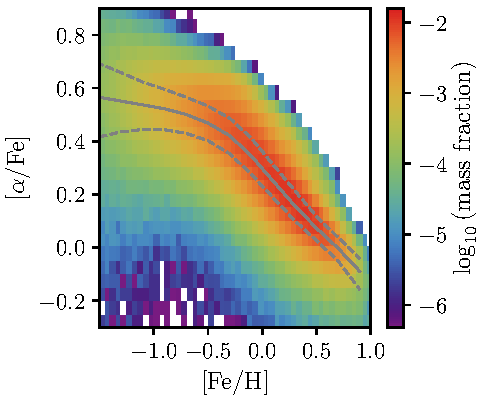
\includegraphics[width=0.6\columnwidth]{L0100N1504_REFERENCE_disks_masshist_largebins.pdf}
\caption[The mass weighted \afe{}-\feh{} distribution of stacked `disc stars' inside Milky Way mass galaxies in the Ref-L100N1504 simulation]{\label{fig:afestack} Two-dimensional histogram of the mass-weighted \afe{}-\feh{} distribution of all `disc stars' associated with the 133 galaxies identified as broad analogues of the Milky Way in terms of their stellar mass and morphology (see Section \ref{sec:disc_stellar_pops}) at $z=0$ in Ref-L100N1504. The overplotted solid line shows the median \afe{} in bins of $\Delta$\feh{}\,$=0.2$, dashed lines show the interquartile range.}
\end{figure}

Fig. \ref{fig:afestack} shows the \afe{}-\feh{} distribution of the 1.5 million stellar particles comprising the disc populations (see Section \ref{sec:disc_stellar_pops}) of the 133 present-day Milky Way-like galaxies in Ref-L100N1504 as a 2-dimensional histogram. The pixels of the histogram represent bins of 0.05 in $\Delta$\afe{} and $\Delta$\feh{}, and the value of each pixel is weighted by the current (rather than initial) mass of the stellar particles within. The overplotted filled line represents the median \afe{} calculated in bins of $\Delta$\feh{}$=0.2$, and the dashed lines show the interquartile range. As has been observed by Galactic surveys, and is commonly predicted by analytic and numerical Galactic chemical evolution models (as expressed in Chapter \ref{sec:discabundances}), the primary trend is that of a sequence with declining \afe{} as a function of \feh{}, with a relatively shallow negative gradient at low \feh{} and steeper gradient at higher \feh{}. The distribution of \afe{} at fixed \feh{} is unimodal, with a broad dispersion. The median \afe{} declines gradually from $0.57$ at \feh{}$\,=-1.0$ to $\simeq 0.47$ at \feh{}$\,=-0.5$, then declines more rapidly to \afe{}$\,\simeq 0.07$ at \feh{}$\,=0.5$. The $1\sigma$ scatter in \afe{} is approximately $0.41$ at \feh{}$\,=-1.0$, and narrows to $0.14$ at \feh{}$\,=0.5$. The increased scatter at low \feh{} is likely a consequence of poor sampling of the enrichment process.

I next turn to an examine the underlying properties of the disc stars, to elucidate the origin of the distribution shown in Fig. \ref{fig:afestack}. The common interpretation for the diversity of \afe{} in the Galaxy's disc stars is a varying relative contribution of Type Ia and Type II SNe ejecta to the Fe abundance of each star. This fraction is tracked explicitly by the simulations, enabling this hypothesis to be tested directly. I examine the same sample of stellar particles shown in Fig. \ref{fig:afestack}, and show in Fig. \ref{fig:afesniafrac} the mean mass fraction of their Fe that was synthesised by Type Ia SNe, $f_{\rm Fe,SNIa}$, as a function of their position in \afe{}-\feh{} space. The mean fraction of each pixel is computed weighting by the current mass of its contributing stellar particles. The mass distribution shown in Fig. \ref{fig:afestack} is illustrated here with overlaid contours, the outer and inner contours corresponding to $\log_{10}{(\mathrm{mass\ fraction})} = -3.5$ and $-2.5\ \mathrm{pixel^{-1}}$, respectively. Only well sampled pixels, with $\log_{10}{(\mathrm{mass\ fraction})} > -4.5\ \mathrm{pixel^{-1}}$, corresponding to approximately 50 stellar particles, are shown.

\begin{figure}
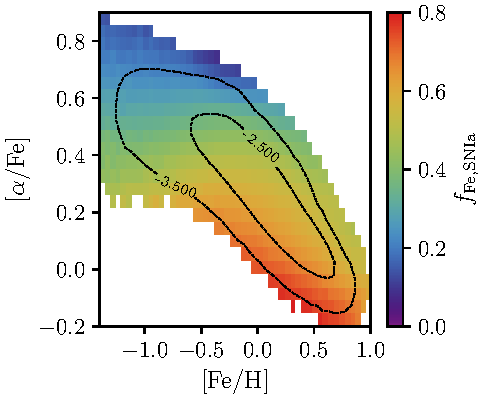
\includegraphics[width=0.6\columnwidth]{L0100N1504_REFERENCE_disks_fefromsniahist.pdf}
\caption[Two-dimensional histogram showing the mean mass fraction of stellar Fe which was ejected by Type Ia SNe, as a function of \afe{} and \feh{} for Ref-L100N1504 disc stars]{\label{fig:afesniafrac} The mean mass fraction of the Fe, locked up in the disc stars of present-day Milky Way-like galaxies in Ref-L100N1504, that was synthesised by Type Ia SNe. The fraction is shown as a function of the stellar populations' position in \afe{}-\feh{} space. The value in each  pixel is weighted by the current mass of the stellar particles within. Overplotted contours reproduce the mass distribution shown in Fig. \ref{fig:afestack}. The Type Ia SNe Fe fraction broadly anti-correlates with \afe{}, and at fixed \afe{} the Fe mass fraction contributed by Type Ia SNe is greatest in Fe-poor stars.}
\end{figure}

As one might expect, there is a broad anti-correlation between \afe{} and $f_{\rm Fe,SNIa}$. According to the simulations the majority of the Fe locked into disc stars with \afe{}$\,\gtrsim 0.5$ was synthesised by Type II SNe, with the mass fraction synthesised in Type Ia SNe being typically $< 0.2$. Conversely, in stars with subsolar \afe{}, which typically exhibit supersolar \feh{}, the mass fraction of Fe synthesised by Type Ia SNe can be $\simeq 0.8$. There is also a weaker, but significant trend at fixed \afe{} ($\lesssim 0.2$), such that stars with higher \feh{} have a smaller Fe contribution from Type Ia SNe. Enrichment of gas by Type II SNe increases \feh{} at broadly fixed \afe{} (a shift to the right in the \afe{}-\feh{} plane) if enrichment by Type Ia is negligible, or whilst increasing \afe{} (a shift up and to the right) if Type Ia enrichment is significant. Enrichment of Type Ia SNe tends to increase \feh{} whilst decreasing \afe{} (a shift down and to the right). Therefore, greater \feh{} at fixed \afe{} is typically due to the more Fe-rich stars sourcing a greater fraction of their Fe from from Type II SNe relative to Type Ia SNe. 

Analytic models posit that high-\afe{} stellar populations form in the early life of a galaxy, and do so rapidly, such that there is little opportunity for the enrichment of star-forming gas by the delayed release of Type Ia SNe ejecta. \citet{2016MNRAS.461L.102S} show that this is the case for the galaxy-averaged $\alpha$-enhancement of massive EAGLE galaxies, whose stars form rapidly at early times prior to quenching by AGN feedback. To examine whether the same applies in Milky Way-like galaxies, I plot in Fig. \ref{fig:afeages} the mean age of stellar particles as a function of their position in \afe{}-\feh{} space, and in Fig. \ref{fig:afetcon} the mean consumption timescale\footnote{The inverse of the consumption timescale is often referred to as the `star formation efficiency' in the chemical evolution modelling literature.} of the natal gas, $t_{\rm g} = \Sigma_{\rm g}/\dot{\Sigma}_\star$, where $\Sigma_{\rm g}$ is the gas surface density and $\dot{\Sigma}_\star$ is the star formation rate (SFR) per unit area. As in previous plots, the pixel values are weighted by the current mass of the stellar particles within, and overlaid contours represent the mass distribution shown in Fig. \ref{fig:afestack}. 

\begin{figure}
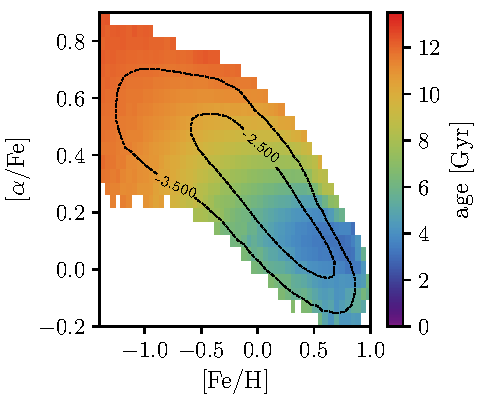
\includegraphics[width=0.6\columnwidth]{L0100N1504_REFERENCE_disks_agehist.pdf}
\caption[Mean stellar age as a function of \afe{} and \feh{} for disc stars in Ref-L100N1504]{\label{fig:afeages} The mean age of the disc stars of present day Milky Way-like galaxies in Ref-L100N1504, as a function of their position in \afe{}-\feh{} space. Pixel values are weighted by the current mass of the stellar particles within, and the overplotted contours reproduce the mass distribution shown in Fig. \ref{fig:afestack}. Age correlates with \afe{}, though at any fixed \afe{} disc stars exhibit a broad range of mean ages, depending on their \feh{}. At fixed \feh{}, the most $\alpha$-rich stellar populations tend to be the oldest.}
\end{figure}

The consumption timescale provides an estimate of the period of time a parcel of star-forming gas resides in the ISM, during which it can be enriched by the ejecta of neighboring stellar populations. It is likely that $t_{\rm g}$ overestimates the time spent in the ISM by a star-forming particle, since it only considers the regulation of the gas surface density by star formation, thus neglecting the influence of feedback. On average, $\langle N_{\rm heat} \rangle \simeq 1$ SPH particle is stochastically heated by the stellar feedback accompanying the formation of each stellar particle, and these particles can entrain neighboring particles in outflows. Outflows can also be driven by AGN feedback, so the accuracy of this estimate is likely poorer than a factor of $\simeq 2$. Nonetheless, $t_{\rm g}$ remains an instructive diagnostic for our purposes. To compute it, I follow \citet{2008MNRAS.383.1210S} and assume that the scale height of star-forming gas discs is comparable to the local Jeans length, $L_{\rm J}$, such that $\Sigma_{\rm g} \simeq \rho_{\rm g}L_{\rm J}$, and then relate the consumption timescale of star-forming gas to its pressure:
\begin{equation}
\label{eq:t_g}
 t_{\rm g} = A^{-1}(1\,{\rm M}_\odot\,{\rm pc}^{-2})^n\left( \frac{\gamma}{G} f_{\rm g}P_\star\right)^{(1-n)/2}.
\end{equation}
Here, $\gamma=5/3$ is the ratio of specific heats for an ideal gas, and $f_{\rm g}$ is the local gas fraction, which I assume to be unity. The parameters $A$ and $n$ are specified by observations, i.e. the Kennicutt-Schmidt scaling relation. I use $A=1.515\times 10^{-4}\,{\rm M}_\odot\,{\rm yr}^{-1}\,{\rm kpc^{-2}}$ and $n=1.4$, with the former being a factor of $1.65$ lower than the value specified by \citet{1998ApJ...498..541K}, since the simulations assume a Chabrier, rather than Salpeter, IMF. For the purposes of the calculation, the pressure of the natal gas, $P_\star$, is assumed to be that specified by the temperature floor described in Section \ref{sec:eagle}, i.e. $P_\star = P_{\rm eos}(\rho_\star)$, where $\rho_\star$ is the density of the natal gas at the instant it is converted into a stellar particle.

Fig. \ref{fig:afeages} shows that, as expected, there is a strong correlation between the present-day age of stellar populations, and their position in \afe{}-\feh{} space. The characteristic age of Fe-poor (\feh{}$\,\lesssim -0.5$), $\alpha$-rich (\afe{}$\,\gtrsim 0.4$) stars is greater than $10\,{\rm Gyr}$, corresponding to a formation redshift of $z \gtrsim 1.7$, whilst those with solar or supersolar iron abundance, for which \afe{}$\,\lesssim 0.2$, are typically younger than $5\,{\rm Gyr}$ ($z_{\rm form} \lesssim 0.5$). There is a clear preference for $\alpha$-rich stars to be old, but disc stars can exhibit a broad range of ages at fixed \afe{}, such that there is not a direct mapping between age and $f_{\rm Fe,SNIa}$. This notwithstanding, at any fixed value of \feh{}, the stars richest in $\alpha$ elements generally tend to be the oldest. 

\begin{figure}
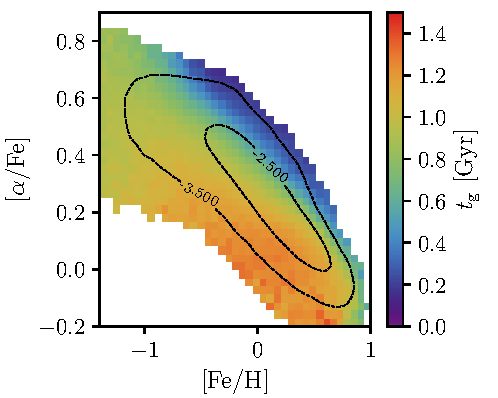
\includegraphics[width=0.6\columnwidth]{L0100N1504_REFERENCE_disks_tconhist_redo.pdf}
\caption[Mean gas consumption timescale as a fucntion of \afe{} and \feh{} for disc stars in Ref-L100N1504]{\label{fig:afetcon} The mean gas consumption timescale $t_{\mathrm{g}}$ of the natal gas from which the disc stars of present-day Milky Way-like galaxies in Ref-L100N1504 formed, as a function of their position in \afe{}-\feh{} space.  Pixel values are weighted by the current mass of the stellar particles within, and the overplotted contours reproduce the mass distribution shown in Fig. \ref{fig:afestack}. At fixed \feh{}, the most $\alpha$-rich stellar particles formed from gas with the shortest consumption timescales.}
\end{figure}

Fig. \ref{fig:afetcon} reveals a striking trend, clearly highlighting that at fixed \feh{} the most $\alpha$-rich populations form from gas that exhibits the shortest consumption timescales. As the dynamic range is narrow for $t_{\rm g} \gtrsim 1\,{\rm Gyr}$, I adopt a linear scaling of colour with $t_{\rm g}$. The plot illustrates clearly that the reason the release of ejecta from Type Ia SNe is able to influence the \afe{} of stellar populations at fixed \feh{} is the fact that the gas consumption timescales are of the same order as the characteristic e-folding timescale of the Type Ia SNe delay time distribution. Although gas can be enriched at densities below the star formation density threshold (whence $t_{\rm g}$ is infinite), the clear connection between $t_{\rm g}$ and (in particular) \afe{} highlights that, for most stellar particles, the bulk of their enrichment must take place whilst they comprise the star-forming ISM. The e-folding timescale of $\tau=2\,{\rm Gyr}$ adopted by the Reference model corresponds to a `half-life' of $t_{1/2}=\tau\ln(2)=1.4\,{\rm Gyr}$. The adoption of a shorter (longer) e-folding timescale results in the advancement (delay) of the release of Fe synthesised by Type Ia SNe, thus inhibiting (promoting) the formation of disc stars with high \afe{}. 

The majority ($\gtrsim 85$ percent) of stellar particles formed from gas with consumption times $\gtrsim 1\,{\rm Gyr}$, but those that formed more rapidly were largely precluded from enrichment by the Type Ia SNe of recently-formed, nearby stellar populations. It is noteworthy that the $t_{\rm g}$ distribution on the \afe{}-\feh{} plane does not map directly onto that of the distribution of $f_{\rm Fe,SNIa}$ shown in Fig. \ref{fig:afesniafrac}. This is because short consumption timescales are realised within gas-rich overdensities at early epochs, and also within massive, metal-rich galaxies at later times.

\subsection{Galaxy-to-galaxy diversity of $\alpha$-enrichment}
\label{sec:afefeh_diversity}

Having examined the distribution of stars in \afe{}-\feh{} space, in a collective sense, for the present-day Milky Way analogues identified in Ref-L100N1504, I now examine the galaxy-to-galaxy diversity of the \afe{}-\feh{} distribution. This exercise enables a first assessment of how common among other present-day disc galaxies is the observed distribution in the \afe{}-\feh{} plane of the Milky Way's disc stars.

\begin{table}
\center
\caption[Properties of three example disc galaxies from the Ref-L100N1504 simulation]{\label{tab:diag} Basic properties of the three present-day galaxies shown in Figure \ref{fig:afeexamples}. The rows correspond to, respectively: the labels applied to each galaxy in the text, their Galaxy ID and FOF ID in public EAGLE galaxy catalogues, their stellar mass, halo mass, their specific star formation rate (sSFR), their  $\kappa_{\mathrm{co}}$ value, and their half-mass radius.}
\begin{tabular}[]{r|rrrl}
\hline
\hline
Label                               & A    & B    & C    &  \\
\hline
Galaxy ID							& 16850421 & 16925427 & 16921468  & \\
FOF ID                              & 507  & 527  & 526  &  \\
$M_{*}$                             & 5.18 & 5.80 & 6.52 & $[10^{10} {\rm M}_{\odot}$] \\
$M_{200}$                           & 2.32 & 2.92 & 3.41 & $[10^{12} {\rm M}_{\odot}$] \\
sSFR                                & 4.74 & 5.14 & 1.85 & [$ 10^{-11} \mathrm{yr^{-1}}$] \\
$\kappa_{\mathrm{co}}$            & 0.67 & 0.45 & 0.46 & \\
$r_{1/2}$                           & 8.83 & 9.49 & 3.00 & [$\mathrm{kpc}$] \\
\hline
\end{tabular}

\end{table}

The present-day \afe{}-\feh{} distributions of the sample of 133 EAGLE galaxies exhibit significant diversity. Based on visual inspection, I have broadly classified the galaxies into the following categories, with the occupancy of each category in parentheses: unimodal with low-\afe{} (82), unimodal with high-\afe{} (19), broad \afe{} at fixed \feh{} (10), ambiguous (22). The sample is therefore dominated by galaxies that exhibit a single, broadly continuous `sequence' that is (unsurprisingly) similar to the overall trend revealed in Fig. \ref{fig:afestack}. A handful of single-sequence galaxies track the upper envelope of the stacked distribution and might reasonably be considered analogous to the stellar populations comprising the high-\afe{} sequence observed in the Galaxy. Six of the 10 galaxies categorised as having broad \afe{} at fixed \feh{} in fact exhibit a clear bimodality in \afe{} at fixed \feh{}, and might be considered, somewhat subjectively, as qualitatively similar to the Galaxy. The sample also includes systems with complex abundance distributions that in some cases are indicative of a recent merger with a gas-rich companion, for example where \afe{} exhibits a positive correlation with \feh{} over a narrow range.

\begin{figure*}
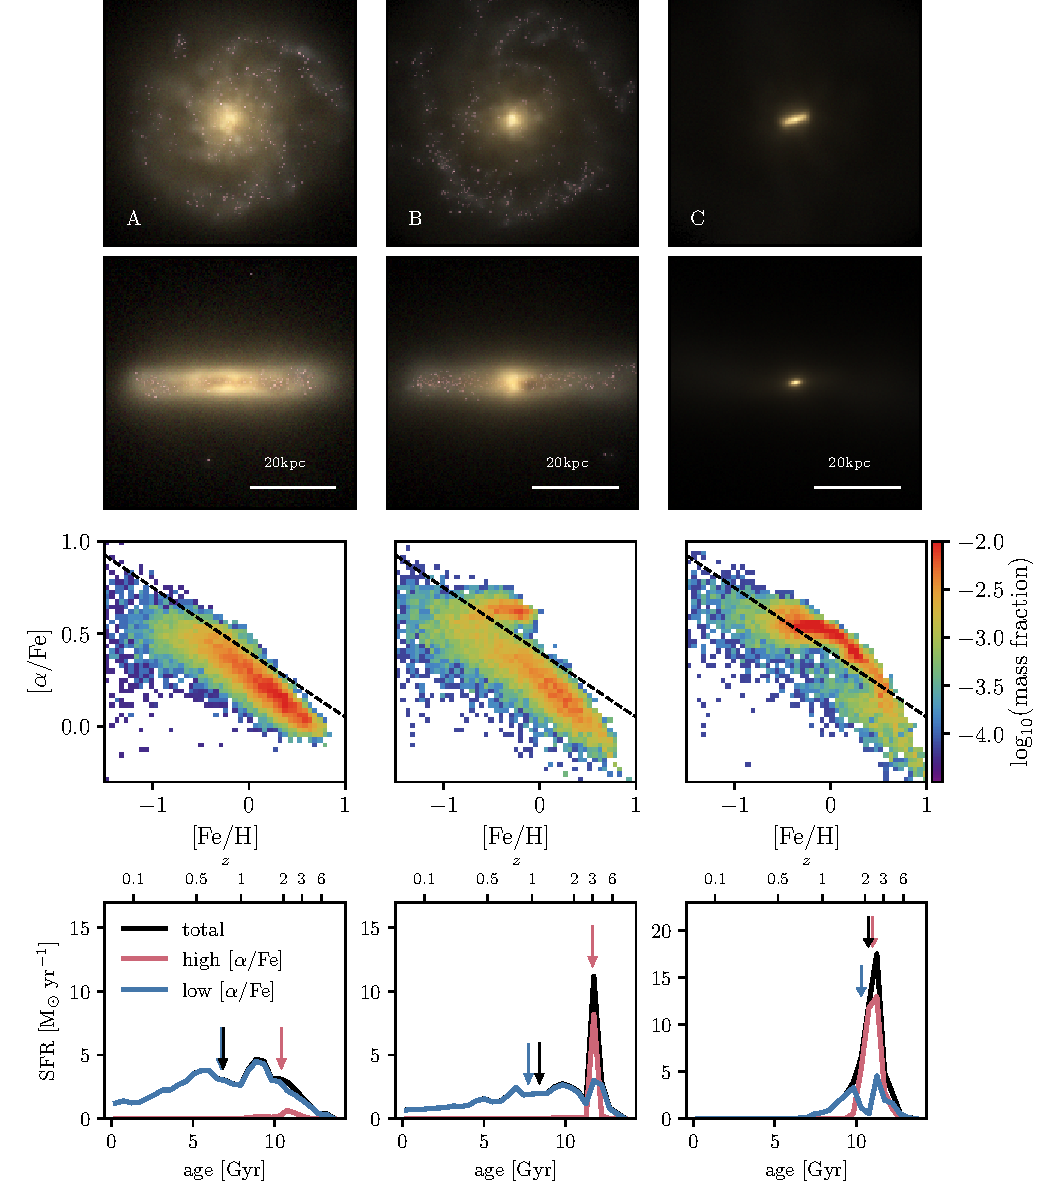
\includegraphics[width=1.\textwidth]{L0100N1504_REFERENCE_afeexamples.pdf}
\caption[Images, \afe{}-\feh{} distributions and star formation histories of three exemplar disc galaxies from the Ref-L100N1504 simulation]{\label{fig:afeexamples} Examples illustrating the diversity of the \afe{}-\feh{} distribution of disc stars from present-day galaxies in Ref-L100N1504. From left to right, the columns correspond to the galaxies labelled A, B and C in the text, for which key properties are quoted in Table \ref{tab:diag}. The two upper rows show mock images of the galaxies, with a $50 \times 50\,{\rm kpc}$ field of view, in the face-on and edge-on orientations. The images show the stellar light based on the combination of monochromatic $u$-, $g$- and $r$-band SDSS filters. The third row shows the \afe{}-\feh{} plane of the disc stars, with the dashed diagonal line positioned to broadly separate the high- and low-\afe{} sequences. This separation enables, in the bottom row, the contribution to the total (\textit{black}) star formation history of the stars comprising the high- (\textit{red}) and low-\afe{} (\textit{blue}) sequences to be shown. Downward arrows denote the epoch by which half of the stellar particles comprising these populations formed.}
\end{figure*}

To illustrate the diversity of the \afe{}-\feh{} distributions, I identify three representative examples: a galaxy exhibiting a single low-\afe{} sequence, a galaxy exhibiting bimodality in \afe{} at fixed \feh{}, and a galaxy exhibiting a single, high-\afe{} sequence. Key properties of these galaxies, labelled A, B and C, respectively, are given in Table \ref{tab:diag}. From top to bottom these are, respectively, the FOF halo identifier of the galaxy in the EAGLE public database\footnote{\url{http://galaxy-catalogue.dur.ac.uk}} \citep{2016A&C....15...72M}; its stellar mass, $M_\star$; its virial mass, $M_{200}$, defined as the total mass (in gas, stars, BHs and dark matter) enclosed by a sphere of radius $R_{200}$, centred on the galaxy's most bound particle, within which the mean enclosed density is $200$ times the critical density, $\rho_{\rm c} \equiv 3H^2/8\pi G$; the specific star formation rate of the galaxy, $\dot{M}_\star/M_\star$; its median kinetic energy in ordered rotation, $\langle \kappa \rangle$; and its stellar half-mass radius, $R_{1/2}$. 

The columns of Fig. \ref{fig:afeexamples}, from left to right respectively, show further properties of A, B and C. The two upper rows show images of the galaxies at $z=0$ with a $50 \times 50\,{\rm kpc}$ field of view, in face-on and edge-on orientation, defined such that the disc plane is orthogonal to the angular momentum axis of the stellar particles within $30\,{\rm kpc}$ of the most-bound particle. The images were extracted from the EAGLE public database, and were created using the techniques described by \citet{2015MNRAS.452.2879T}. The third row presents the \afe{}-\feh{} distribution of the disc stars, shown as a mass-weighted 2-dimensional histogram. The dashed diagonal line is an arbitrary threshold chosen to separate the high- and low-\afe{} sequences, which enables the contribution to the star formation history of the particles comprising each sequence to be shown separately in the bottom row. The downward arrows denote the epoch by which half of the stellar particles comprising the populations formed. 

Galaxies A and B exhibit a classical structure, with a central red spheroid surrounded by an extended blue disc. The spheroid of galaxy A is relatively diffuse, whilst that of galaxy B is more massive and more compact. Galaxy C is dominated by a central, rapidly-rotating elongated spheroid, and is an example of the relatively rare cases for which a high value of $\langle \kappa \rangle$ does not correspond to a morphologically-extended disc \citep[see][]{2017arXiv170406283C}. The bulk of galaxy A's disc stars form a continuous sequence in \afe{}-\feh{} space, at a relatively low value of \afe{}, extending to \feh{}$\,\simeq 0.8$. A similar sequence is visible in the case of galaxy B, extending almost to \feh{}$\,\simeq 1$. This low-\afe{} sequence is supplemented by an $\alpha$-rich (\afe{}$\,\simeq 0.65$) sequence that extends to  \feh{}$\,\simeq 0$. Galaxy C is dominated by a high-\afe{} sequence that is approximately constant at \afe{}$\,\simeq 0.6$ until \feh{}$\,\simeq 0$, and gradually declines as a function of increasing \feh{}. A small fraction of galaxy C's disc stars populate a region of \afe{}-\feh{} space similar to galaxy B's low-\afe{} sequence at the highest values of \feh{}.

The formation histories of the stars comprising the high and low \afe{} sequences (or lack thereof) offer clues to their origin. Galaxy A exhibits an extended star formation history that evolves smoothly between values of $1-5\,{\rm M}_\odot\,{\rm yr}^{-1}$. This history is consistent with relatively long consumption timescales ($\gtrsim 1\,{\rm Gyr}$), and yields a relatively young stellar disc (an initial mass-weighted mean age of $7\ {\rm Gyr})$. The low-\afe{} component of galaxy B behaves similarly, albeit at a slightly lower SFR than galaxy A. The formation of galaxy B's high-$\alpha$ component dominates the early stages of its disc formation, and during this period of rapid star formation the SFR peaks at $\dot{M}_\star > 10\,{\rm M}_\odot {\rm yr}^{-1}$. The stars comprising this sequence therefore formed with an initial mass-weighed mean consumption time of $t_{\rm g} \simeq 200\ {\rm Myr}$. Nearly all of the stellar particles comprising the high-\afe{} sequence are formed during this episode. The formation of galaxy C is similar to the early behaviour of galaxy B, albeit more extreme. The massive, concentrated spheroid forms in a single, extended episode of rapid star formation during which the SFR peaks at $\dot{M}_\star \simeq 17\,{\rm M}_\odot {\rm yr}^{-1}$, yielding a initial mass-weighed mean consumption time of  $t_{\rm g} \simeq 180\ {\rm Myr}$. 

The star formation histories of these examples therefore corroborate the broad picture inferred from inspection of Figs. \ref{fig:afesniafrac}, \ref{fig:afeages} and \ref{fig:afetcon}: high values of \afe{} are realised by stellar populations with only a small fraction of their Fe mass synthesised by Type Ia SNe. Such populations are typically formed at early cosmic epochs, from gas with $t_{\rm g} < \tau$. This close connection between the star formation history and the distribution of stars in the \afe{}-\feh{} plane highlights that the former could be `reverse engineered' by applying analytic chemical evolution models to measurements of the latter, but the conclusions drawn from such an exercise might not be generally applicable to the broader population of galaxies with similar mass and morphology. 

\section{The origin of the \afe{}-\feh{} distribution of disc stars}
\label{sec:afeorigin}

In this section I examine the evolution of the \emph{gas} from which the stellar populations occupying specific regions of the \afe{}-\feh{} plane formed. I also examine the subsequent radial migration of these populations within the disc. I begin by analysing a single galaxy, and generalise the analysis to the broader population in Section \ref{sec:broader_applicability}.

\begin{figure*}
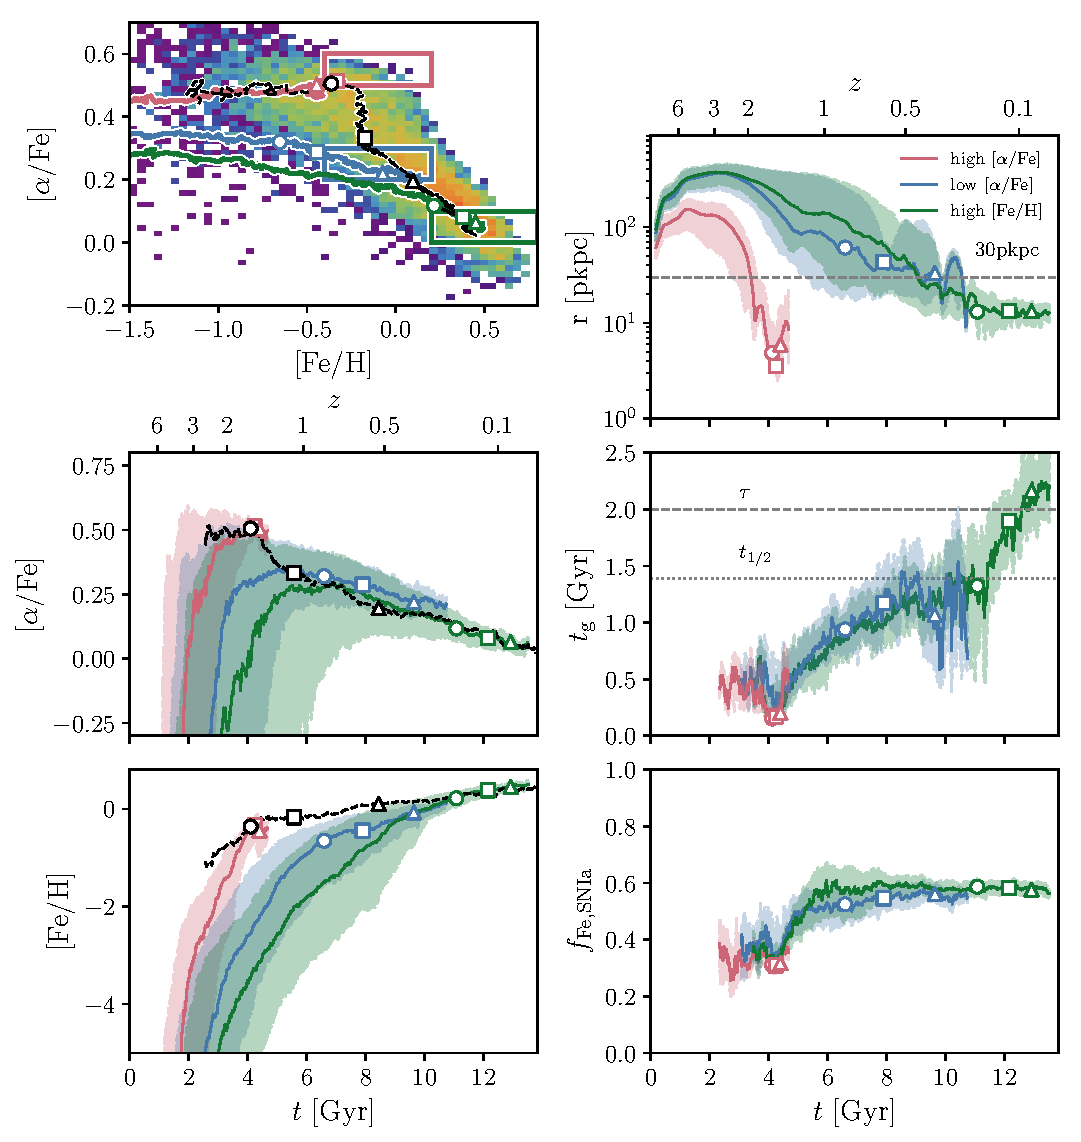
\includegraphics[width=\textwidth]{L0025N0376_REFERENCE_ApogeeRun_FOF17_megaplot.pdf}
\caption[The history of gas (in various parameters) which forms the stellar populations of an example disc galaxy taken from the Ref-L025N0376 Simulation]{\label{fig:daddyplot} The enrichment history of the natal gas of disc stars occupying selected regions of the $z=0$ \afe{}-\feh{} plane, for the galaxy discussed in Section \ref{sec:afeorigin}. The upper-left panel shows the mass distribution of stars in the \afe{}-\feh{} plane. Particle selections corresponding to "high-\afe{}", "low-\afe{}" and "high-\feh{}" are denoted by the overlaid red, blue and green boxes, respectively. Overlaid coloured tracks denote the evolution of the median abundances of the natal gas of these populations, with circle, square and triangle symbols corresponding to the epochs at which 25, 50 and 75 percent of the gas has been consumed, respectively. The evolution of the median \afe{} and \feh{} is plotted as a function of cosmic time in the centre-left and lower-left panels, respectively. Shaded regions on these panels denote the interquartile range. Dashed black tracks on the panels of the left-hand column denotes the SFR-weighted median gas-phase abundances. The upper-right panel shows the evolving median and interquartile range of the galactocentric radii (in proper coordinates) of the natal gas of each population. The centre-right panel shows the SFR-weighted mean consumption time of the natal gas, and the bottom-right panel shows the SFR-weighted mean of the natal gas mass fraction of Fe that was synthesised by Type Ia SNe. For these two panels, the shaded regions denote the $1\sigma$ scatter about the mean.}
\end{figure*}

The Lagrangian nature of the EAGLE simulations enables us to reconstruct the full enrichment history of the gas from which disc stars formed. It is therefore instructive to examine the evolution of the elemental abundances of the `natal' gas of the stars occupying key positions in the \afe{}-\feh{} plane at $z=0$. Although, as discussed in Section \ref{sec:subgrid_physics}, the mass and metals donated by stellar particles to SPH particles are `fixed' to particles and do not diffuse between them, any dilution of elemental abundances resulting from the inflow of low-metallicity gas can nonetheless be captured, since I examine kernel-smoothed abundances. In order to examine enrichment histories with superior temporal resolution to that afforded by the standard set of EAGLE snapshots, I focus here on the Ref-L025N0376 simulation, for which 1000 snapshots were recorded. One of the galaxies that forms in this simulation is, at $z=0$, a disc-dominated ($ \kappa_{\mathrm{co}} = 0.58$, $r_{1/2} = 8.8$ kpc) central galaxy that exhibits \afe{} bimodality at fixed \feh{}. Its stellar mass is $M_{*} = 4.58\times 10^{10}\mathrm{M_{\odot}}$, slightly below the lower bound of the mass interval used in Section \ref{sec:disc_stellar_pops} to define the Ref-L100N1504 sample, but this galaxy is a useful example owing to the similarity of its star formation history and elemental abundances with those of galaxy B. Its present-day halo mass is $M_{200} = 2.54\times 10^{12}\mathrm{M_{\odot}}$.

Fig. \ref{fig:daddyplot} summarises the enrichment history of this galaxy. The upper-left panel shows the \afe{}-\feh{} distribution of the galaxy's present-day disc stars as a 2-dimensional histogram. The overlaid boxes define three populations of stellar particles, for which the enrichment history of their natal gas particles is reconstructed. The boxes span $\Delta$\feh{}\,$=0.6$ and $\Delta$\afe{}\,$=0.1$, and the red and blue cases, respectively, correspond to high-\afe{} and low-\afe{} at the intermediate values of \feh{} for which the bimodality is most pronounced. The green case corresponds to the greatest values of \feh{}. The three samples comprise between approximately 400 and 900 stellar particles. The overlaid tracks of the same colour show the evolution, for each population, of the median \afe{} and \feh{} abundances of the gas particles that remain unconsumed by star formation. To avoid poor sampling of the measurement, the tracks truncate when only 30 gas particles remain unconsumed, and the evolution of the consumed fraction is shown via the symbols overlaid on each track, which denote the epochs at which 25 percent (circle), 50 percent (square) and 75 percent (triangle) of the gas particles have been consumed (these conditions apply to all tracks presented in this figure). Star formation does not uniformly sample the natal gas, so the elemental abundances of stars formed at a given epoch are not represented by the corresponding position on the median tracks; the dashed black track therefore shows the evolution of the SFR-weighted mean coordinate in \afe{}-\feh{} space. The tracks begin when at least 30 particles have a non-zero SFR. I stress that this track does not represent the enrichment history of any particular gas population, but rather the characteristic elemental abundances with which stars are being formed at the corresponding epoch.

It is immediately apparent that the enrichment histories of the natal gas of the high- and low-\afe{} populations are markedly different. They differ in \afe{} already at very low \feh{}, and the difference grows as the populations become more metal rich. The high-\feh{} population exhibits a similar enrichment history to the low-\afe{} population, but is offset to lower \afe{}; it is accreted at late times (as I discuss later, much of it is delivered by a gas-rich satellite) and enriches to high-\feh{} as it mixes with the interstellar gas of the evolved galaxy. The dashed black track shows that at early times, the $z=0$ disc stars of this galaxy initially form with elevated $\alpha$-elemental abundances and an increasing \feh{}, resulting in the formation of the high-\afe{} sequence. Once a little over 25 percent of all present day disc stars have formed, the formation of high-\afe{} stars begins to subside and the low-\afe{} sequence also begins to emerge. At this epoch the SFR-weighted mean track necessarily declines (and does so at roughly fixed \feh{}), and subsequently converges with the low-\afe{} sequence.

The clear and persistent separation of the median abundances of the natal gas of the high- and low-\afe{} populations signals that they never mixed. In contrast to a central assumption of the two-infall model, at no stage of its evolution does the natal gas of the low-\afe{} sequence reach values of \afe{} that are characteristic of the high-\afe{} population. Hence, rather than subsequently declining to roughly solar \afe{} in response to enrichment by Type Ia SNe ejecta, it simply never reaches values of \afe{} as elevated as those realised by the natal gas of the high-\afe{} population. 

The contrasting enrichment histories of the two gas populations are made more apparent by inspection of the centre-left and bottom-left panels of Fig. \ref{fig:daddyplot}. Respectively, these show the temporal evolution of \afe{} and \feh{}, with the thick solid lines denoting median values and the shaded regions the interquartile range. As with the upper-left panel, since star formation samples a very unrepresentative subset of the gas comprising each population, I stress that the coloured tracks do not denote the typical abundances with which the stars of each population form at the corresponding epoch. To give a sense of how the median abundances of each population differ from the latter, we again show the galaxy's SFR-weighted mean abundance as a dashed black track. All three gas populations \emph{do} initially become $\alpha$-enriched in response to early star formation; the natal gas of the high-\afe{} stars is rapidly enriched to \afe{}$\,\simeq 0.5$ and \feh{}$\,\simeq -0.5$, and is mostly consumed by $t\simeq 4\,{\rm Gyr}$. After its initial enrichment with $\alpha$-elements, the low-\afe{} population's natal gas settles to a value of \afe{}$\,\simeq 0.35$ at $t\simeq 5\,{\rm Gyr}$ ($z \simeq 1.5$), after which it is steadily enriched by Type Ia SNe as it is consumed. This gradually reduces its \afe{}, and increases its \feh{}, in a broadly monotonic fashion. The evolution of \feh{} for this population is much more gradual than is the case for the natal gas of the high-\afe{} stars, the latter reaching \feh{}$\,\gtrsim -0.5$ more than $3\,{\rm Gyr}$ sooner than the former. The correspondence of the high-\feh{} population with the low-\afe{} population is also apparent from inspection of the time evolution of \afe{} and \feh{}. The high-\feh{} population represents the late-infalling subset of the overall low-\afe{} sequence, resulting in a lower abundance of $\alpha$ elements and a higher abundance of Fe. 

It can be concluded from analysis of this galaxy that the elemental abundances of the natal gas of its high- and low-\afe{} populations evolved along distinct paths. Although the latter briefly exhibits elevated \afe{} at early times, which subsequently declines in response to enrichment by Type Ia SNe, this gas never reaches \afe{} comparable to that of the stars comprising the high-\afe{} sequence. The formation of the high-\afe{} sequence is therefore not imprinted in the abundances of the gas from which the low-\afe{} sequence subsequently forms, as one might expect if, as postulated by the two-infall model, the low-\afe{} sequence forms from a mixture of gas accreted from the intergalactic medium and interstellar gas remaining after an initial episode of star formation. This notwithstanding, the characteristic $\alpha$-element and Fe abundances with which stars form, quantified by the mean SFR-weighted coordinate in \afe{}-\feh{} space, does evolve in a fashion that is qualitatively similar to the expectations of the two-infall model: the typical \afe{} declines rapidly as the formation of the high-\afe{} sequence draws to a close and the low-\afe{} sequence begins to dominate. However, as was also noted recently by \citet{2017arXiv170807834G} following analysis of the Auriga simulations, the continuous increase of \feh{} of the natal gas of all populations is incompatible with a key expectation of the two-infall model, namely that the metallicity of the gas from which the Milky Way's disc stars are formed converges towards an equilibrium value.

The dissimilar evolutionary histories of the natal gas of the stars comprising high- and low-\afe{} sequences implies that the gas remained physically separated, and hence chemically independent, prior to its consumption by star formation. This suggests that they accreted onto the galaxy at different times. To explore this possibility, I crudely reconstruct the collapse history of the natal gas of the three populations defined in the upper-left panel of Fig. \ref{fig:daddyplot}. This is achieved by computing the spherical galactocentric radii of the unconsumed gas particles as a function of cosmic time, relative to the coordinate of the most-bound particle of the galaxy's main progenitor subhalo. The resulting trajectories are shown in the upper-right panel, with the tracks denoting the median radius and the shading denoting the interquartile range. The plot adopts proper (rather than comoving) coordinates, to highlight the expansion of gas with the Hubble flow at epochs prior to turnaround, and the horizontal dotted line at $30\,{\rm pkpc}$ provides a threshold below which I consider the gas to have accreted onto the galaxy; this definition is consistent with that used in Section \ref{sec:finding_galaxies}. I further stress that, since star formation does not uniformly sample the gas comprising each population, the median tracks \emph{do not} denote the typical radius at which stars form at each epoch;  an SFR-weighted track is not included here, as the value is always $\ll 30\,{\rm pkpc}$. 

The high-\afe{} population reaches its radius of maximum expansion (the "turnaround radius") earlier ($t\simeq 1\,{\rm Gyr}$) than the low-\afe{} population ($t\simeq 2\,{\rm Gyr}$), and does so at a median galactocentric radius that is more than a factor of two smaller. A significant fraction of natal gas of the low-\afe{} population is delivered by a gas-rich satellite at $t\simeq 10\,{\rm Gyr}$, which induces the oscillatory structure in its median radius. The natal gas of the high- and low-\afe{} populations is in general not co-spatial, precluding significant mixing of their kernel-smoothed element abundances: the median galactocentric radius of the high-\afe{} population drops below $30\,{\rm pkpc}$ at $t=3.4\,{\rm Gyr}$, at which time only 3 percent of the particles comprising the low-\afe{} population are located within $30\,{\rm pkpc}$. The median galactocentric radius of the latter falls below $30\,{\rm pkpc}$ much later, at $t\simeq 9\,{\rm Gyr}$, by which time all of the high-\afe{} population's stars have already formed. 

The influence of the accretion history on the enrichment of these populations is made clear by the centre-right and bottom-right panels of Fig. \ref{fig:daddyplot}. The former shows the evolution of the consumption timescale, $t_{\rm g}$, of the gas, the latter shows the evolution of the gas-phase mass fraction of Fe synthesised by Type Ia SNe $f_{\rm Fe,SNIa}$. Here, $t_{\rm g}$ is computed as per Equation \ref{eq:t_g}, replacing $P_\star$ by the gas particle's pressure. For consistency with Fig. \ref{fig:afetcon}, I assume this to be the equation of state pressure corresponding to the density of the gas, $P_{\rm eos}(\rho)$. Since I am specifically concerned in these two panels with the subset of the gas sampled by star formation, the coloured tracks here show the SFR-weighted mean of the quantity in question, and they begin when at least 30 particles have a non-zero SFR. The shaded regions show the $16^{\rm th}-84^{\rm th}$ percentile scatter, as an estimate of the $1\sigma$ scatter about the mean. 

The early collapse of the natal gas of the high-\afe{} population drives it to high densities and pressures, fostering its rapid conversion to stellar particles with a characteristic consumption timescale that is typically $t_{\rm g} \lesssim 500\,{\rm Myr}$, and hence much shorter than the e-folding ($\tau=2\,{\rm Gyr}$, upper dashed line) and half-life ($t_{1/2}=\tau\log(2)=1.39\,{\rm Gyr}$, lower dotted line) timescales of the Type Ia SNe delay time function. In contrast, over 75 percent of the stars comprising the low-\afe{} sequence (and nearly all of the high-\feh{} stars) form from gas with a consumption timescale of $t_{\rm g} \gtrsim 1.0\,{\rm Gyr}$. The influence of this dichotomy on the enrichment of star-forming gas by Type Ia SNe is then clear from inspection of the bottom-right panel of Fig \ref{fig:daddyplot}. At early epochs, when the high-\afe{} stars form, the typical fraction is $f_{\rm Fe,SNIa} \simeq 0.35$. At $t \gtrsim 4\,{\rm Gyr}$ there is a clear jump in the typical Fe mass fraction from Type Ia SNe, with the low-\afe{} and high-\feh{} populations, which largely form after this transition, typically exhibiting $f_{\rm Fe,SNIa} \simeq 0.55$.

\begin{figure}
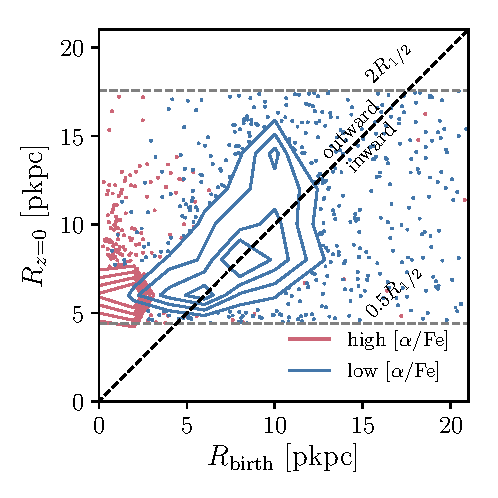
\includegraphics[width=0.6\columnwidth]{L0025N0376_REFERENCE_ApogeeRun_FOF17_newrvsr_scatter+contour.pdf}
\caption[The change in cylindrical radius since birth of disc stars in the example galaxy from Ref-L025N376]{\label{fig:birth_vs_z0_radii} The cylindrical radii at the present day, $R_{z=0}$, of the stellar particles comprising the high- (red) and low-\afe{} (blue) populations of the example galaxy from Ref-L025N0376, as a function of their cylindrical radii at birth, $R_{\rm birth}$. The distribution is shown with contours denoting the levels containing 50, 60, 70 and 80\% of the points, with individual particles drawn beyond the outer (80\%) contour. Grey dashed lines at $R_{z=0} = 0.5R_{1/2}$ and $R_{z=0} = 2R_{1/2}$ show the cylindrical radial boundaries used to define the disc stars, and the black dashed line denotes the locus $R_{z=0} = R_{\rm birth}$. The low-\afe{} population has experienced mild outward radial migration, albeit with large scatter. The high-\afe{} population has necessarily experienced significant outward radial migration in order to be identified as part of the disc, since these stars formed almost exclusively within $5\,{\rm pkpc}$ of the galactic centre.}
\end{figure}

Returning briefly to the upper-right panel of Fig. \ref{fig:daddyplot}, it is striking that the gas from which the stars comprising the high-\afe{} sequence formed was significantly more compact prior to its consumption than was the gas that fuelled the formation of the low-\afe{} stars. This is perhaps to be expected; linear tidal torque theory \citep{1984ApJ...286...38W,1996MNRAS.282..455C} posits that the angular momentum of matter grows whilst it expands with the Hubble flow ($L \propto a^{3/2}$), and remains constant after turnaround. Gas that reaches its radius of maximum expansion later is therefore expected to build more angular momentum, and settle farther out in the galaxy disc. This raises the question of how the stars of both the high- and low-\afe{} populations came to be broadly co-spatial at the present day. 

Fig. \ref{fig:birth_vs_z0_radii} plots the distribution of the present-day cylindrical galactocentric radius of the high- and low-\afe{} stars, $R_{\rm z=0}$, of the example galaxy from Ref-L025N0376, as a function of their cylindrical galactocentric radius at birth, $R_{\rm birth}$. Horizontal dashed lines denote $0.5R_{1/2}$ and $2R_{1/2}$, the cylindrical radial boundaries that are imposed to select disc stars at $z=0$, whilst the black dashed line denotes the locus $R_{z=0} = R_{\rm birth}$. The low-\afe{} population generally tracks this locus, albeit with a large scatter such that significant positive and negative migration is common. Overall there is a mild preference for net positive migration. In contrast, the high-\afe{} population of this galaxy forms almost entirely at $R_{\rm birth} < 3\,{\rm pkpc}$, which is likely a necessary condition in order to realise the short consumption timescales that preclude the enrichment of their natal gas with Type Ia SNe ejecta. Positive outward migration of these stellar particles is therefore necessary in order for them to be categorised as part of the (geometric) disc. 

Isolating the physical cause of this migration is beyond the scope of this study. I note that the limited resolution of the simulations, and their implicit treatment of the cold interstellar gas phase, preclude an examination of whether such migration might be dominated by the `blurring' or `churning' processes discussed by \citet{2009MNRAS.396..203S}. That notwithstanding, as recently argued by \citet{2017arXiv170901040N} following analysis of the high-resolution APOSTLE simulations \citep{2016MNRAS.457.1931S} that also use the EAGLE galaxy formation model, dynamical effects similar to those expected to follow from detailed internal processes can also arise in response to the evolution of the ISM from a `thick' state at early times to a more settled state at low redshift, as the accretion of gas onto (and ejection of gas from) galaxy discs declines \citep[see also][]{2004ApJ...612..894B,2012MNRAS.426..690B,2013ApJ...773...43B,2016arXiv160804133M}.



\subsection{Applicability to galaxies in the Ref-L100N1504 simulation}
\label{sec:broader_applicability}

Visual inspection of the \afe{}-\feh{} planes of the 133 EAGLE galaxies in the sample reveals six that exhibit two clearly-separated sequences in \afe{}-\feh{} space. The \afe{}-\feh{} distributions of these galaxies are shown in the left-hand column of Fig. \ref{fig:bimodalexamples}. In a similar fashion to the case discussed in Section~\ref{sec:afeorigin}, I split the population of disc stars of these galaxies into high- and low-\afe{} sequences, to examine their evolution separately. These examples exhibit a diversity of \afe{}-\feh{} morphologies, so I adopt simple, visually-defined cuts that assign all disc stars to one of the two sequences, as indicated by the dashed lines on each panel. The cuts are defined such that they best separate the sequences where they are well separated. The overlaid tracks and symbols are defined as per the top-left panel of Fig. \ref{fig:daddyplot}. Similarly, the centre column shows the collapse histories of the gas from which the two populations formed, as per the upper-right panel of Fig. \ref{fig:daddyplot}. I discuss the right-hand column later in Section \ref{sec:halo_accretion}.

\begin{figure*}
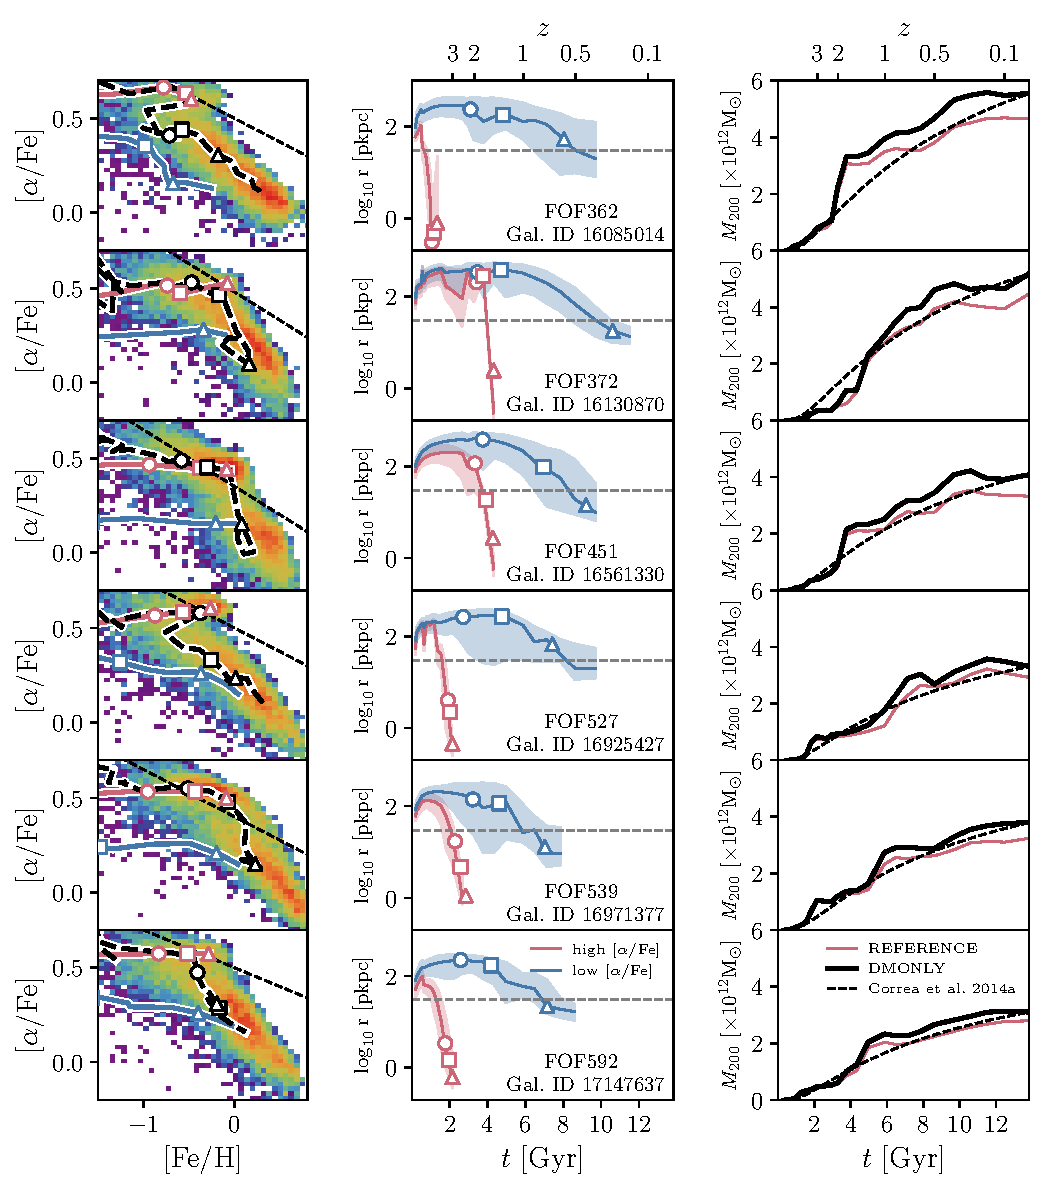
\includegraphics[width=0.95\textwidth]{L0100N1504_REFERENCE_disks_bimodalgallery_rvst_portrait.pdf}
\caption[Evolution of six example galaxies from Ref-L100N1504 which demonstrate bimodality in \afe{} at fixed \feh{}] {\label{fig:bimodalexamples} The evolution of the six galaxies from Ref-L100N1504 that exhibit bimodality in \afe{} at fixed \feh{}. Similarly to Fig. \ref{fig:daddyplot}, the left-hand column shows the \afe{}-\feh{} distribution of the disc stars of these galaxies as a 2-dimensional histogram. Here the disc stars are split into high- and low-\afe{} populations with a simple visually-defined cut, shown by the thin dashed line. The centre column shows the expansion, collapse and accretion onto the galaxy of the natal gas of these two populations. The right-hand column, discussed in Section \ref{sec:halo_accretion}, shows the total mass accretion history of the galaxies, i.e. $M_{200}(t)$. The red curve shows this quantity within the Ref-L100N1504 simulation, whilst the black curve denote the evolution of the same halo identified in its dark matter-only counterpart, DMONLY-L100N1504. Here, the dashed black curve denotes the typical accretion history of haloes with the same present-day mass as the DMONLY realisation of the halo, as parametrised by \citet{2015MNRAS.450.1514C}.} 
\end{figure*}

These panels reveal illuminating features, similarities and differences with respect to the example in Fig. \ref{fig:daddyplot}. As in that Figure, the natal gas populations of the stars comprising the high- and low-\afe{} sequences exhibit distinct enrichment histories, implying a general lack of mixing of their element abundances prior to their consumption by star formation. In all cases, the natal gas of the high-\afe{} sequence reaches a relatively short radius of maximum expansion, "turning around" and accreting onto the galaxy significantly earlier than that of the low-\afe{} sequence. This early collapse enables rapid formation of the high-\afe{} sequence, with the short consumption timescales necessary to inhibit enrichment by the ejecta of Type Ia SNe. As might be expected, the most $\alpha$-rich sequences are formed by the galaxies for which the natal gas collapses at the earliest epochs (FOF362, FOF527 and FOF592), whilst the example for which the natal gas of the two sequences is the most cospatial prior to its accretion onto the galaxy (FOF372) exhibits the least well-separated sequences in \afe{}-\feh{} space. The galaxies also exhibit diversity in the maximum \feh{} abundance to which the high-\afe{} sequence extends; as expected, I find that this is correlated to the mass of stars formed from the gas delivered in the initial episode.

The track of the mean SFR-weighted element abundances exhibits significant diversity, reflecting the non-trivial enrichment evolution of the \emph{star-forming} ISM. The tracks for galaxies FOF 362 and FOF527 illustrate that, as the formation of the high-\afe{} sequence concludes and the formation of low-\afe{} stars begins to dominate, the decline of the characteristic \afe{} is accompanied by a temporary decrease in the characteristic Fe abundance with which new stars are formed (by $\Delta\mathrm{[Fe/H]}\lesssim -0.5$). This indicates that, as posited by the two-infall model, in these two cases the accretion of unenriched gas temporarily lowers the metallicity of the star-forming ISM. Conversely, in the other four bimodal galaxies, the decrease in \afe{} associated with the transition from the high- to low-\afe{} sequence is accompanied by mild increase in \feh{}. 

\section{Connecting disc star element abundances to halo mass accretion histories}
\label{sec:halo_accretion}

The analyses presented in Section \ref{sec:afeorigin} show that distinct sequences in \afe{}-\feh{} space arise in galaxies where disc stars are formed from gas that was accreted onto the galaxy in somewhat separated episodes. Since the accretion of gas is primarily driven by the gravitational evolution of a galaxy's dark matter halo \citep{2008MNRAS.388.1792N,2010MNRAS.406.2267F,2015MNRAS.450.1521C,2015MNRAS.450.1514C,2015MNRAS.452.1217C}, this finding highlights that the distribution of disc stars in the \afe{}-\feh{} plane is influenced not only by astrophysical processes, but perhaps more fundamentally by the hierarchical formation and assembly of the galaxy. I therefore briefly examine in this section the connection between bimodality in \afe{} at fixed \feh{}, and the accretion history of a galaxy's dark matter halo.

The right-hand column of Fig. \ref{fig:bimodalexamples} shows the total mass accretion history of the six bimodal galaxies discussed in Section \ref{sec:broader_applicability}, characterised by the evolution of the halo virial mass, $M_{200}(t)$. In each case, the red curve shows growth of the virial mass of the halo within the Ref-L100N1504 simulation. The thick solid curve shows the evolution of $M_{200}^{\rm DMO}(t)$, the virial mass of the same halo, identified using the techniques described by \citet{2015MNRAS.453L..58S}, in a simulation of the L100N1504 volume considering only collisionless gravitational dynamics (DMONLY-L100N1504). This track is instructive as it eliminates the influence of astrophysical processes associated with baryons, such as adiabatic contraction, which acts to increase the central density of the halo, and the reduction of the halo's mass and accretion rate due to the ejection of baryons by feedback processes. The dashed curve shows the typical accretion history of a halo with the same present-day mass as the halo in the DMONLY-L100N1504 simulation, as derived by \citet{2015MNRAS.450.1514C} through application of the extended Press-Schechter (EPS) formalism to the growth rate of initial density perturbations.

The importance of accounting for the influence of baryon physics, in particular ejective feedback, is made clear by comparison of the Reference and DMONLY curves. In each case, these curves diverge significantly at intermediate redshifts ($1 \lesssim z \lesssim 3$). As shown by \citet[][their Fig. 1]{2015MNRAS.453L..58S}, the median of the ratio $M_{200}/M_{200}^{\rm DMO}$ at $z=0$ is $\simeq 0.85$ for haloes of $M_{200}^{\rm DMO} \sim 10^{12}-10^{13}\,{\rm M}_\odot$  Comparison of the DMONLY curves with the \citet{2015MNRAS.450.1514C} fitting function reveals that a common feature of the mass accretion histories of the 6 bimodal galaxies is rapid growth at early times ($4 \lesssim t \lesssim 6\,{\rm Gyr}$ or $1 \lesssim z \lesssim 2$), such that early in their assembly, they grow faster than is typical for haloes of the same present-day mass. Their accretion rate subsequently declines relative to the average rate for haloes of the same z=0 mass, such that at late times $M_{200}^{\rm DMO}(t)$ grows at a significantly \textit{lower} rate than is typical. Na\"ively, an elevated mass accretion rate at early cosmic epochs is qualitatively consistent with the early collapse of the gas that fuels the formation of the high-\afe{} sequence. This also motivates the question of whether the haloes that host disc-dominated galaxies with distinct sequences in \afe{}-\feh{} space differ significantly and systematically from those hosting disc-dominated galaxies with unimodal \afe{}-\feh{} distributions. 

\begin{figure}
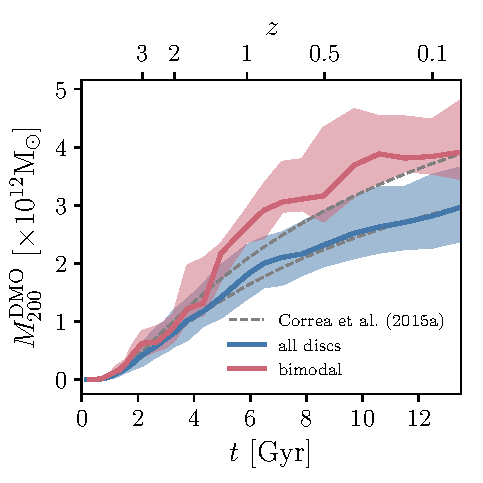
\includegraphics[width=0.5\columnwidth]{L0100N1504_DMONLY_disks_accretionhistory_m200_unnorm.pdf}
\caption[Mass accretion history of \afe{}-bimodal haloes in the DMONLY-L100N1504 simulation, compared to the accretion history of haloes hosting galaxies at the same stellar mass which do not show the same bimodality]{\label{fig:comp_uni_bi_acc_hist} The mass accretion history, $M_{200}(t)$, of haloes identified in the DMONLY-L100N1504 simulation. The thick curves corresponds to the median, whilst the shaded regions denote the interquartile range. The blue curve corresponds to the partner haloes of all 133 galaxies in the Milky Way-like sample, whilst the red curve corresponds to the partner haloes of the 6 galaxies exhibiting bimodality in \afe{} at fixed \feh{}. Dashed curves meeting the two median curves at $z=0$ show the typical accretion history, as parametrised by \citep{2015MNRAS.450.1514C}, of haloes with these $z=0$ masses. Haloes which host galaxies exhibiting \afe{} bimodality have systematically different dark matter accretion histories}
\end{figure}

I therefore identify the DMONLY counterpart haloes of all 133 Milky Way-like galaxies in Ref-L100N1504. We plot in Fig. \ref{fig:comp_uni_bi_acc_hist} the median and interquartile range of $M_{200}^{\rm DMO}(t)$ derived from these samples (blue curves denote the entire sample, red curves denote the six bimodal galaxies). As per the right-hand column of Fig. \ref{fig:bimodalexamples}, the overlaid dashed curves that intersect the median curves at $z=0$ denote the typical accretion histories, as parametrised by Correa et al. (2017a), of haloes with the same present-day mass. Comparison of the two median tracks indicates that the phase of rapid growth exhibited by bimodal galaxies between $t \simeq 4$ and $t \simeq 8\,{\rm Gyr}$ (corresponding to $z \simeq 1.6$ and $z \simeq 0.5$) is not common amongst the broader population of Milky Way-like galaxies. In general, the latter exhibit accretion histories that are much more representative of the entire population of haloes with similar present-day mass. It can therefore be concluded that the accretion histories of bimodal galaxies are indeed atypical. I note that the present day halo masses of the bimodal galaxies are not representative of the overall distribution; the median $M_{200}^{\rm DMO}(z=0)$ of the bimodal galaxies is equal to the $80^{\rm th}$ percentile of that of the overall sample of Milky Way-like galaxies. However, I have verified that median accretion history of the latter remains largely unchanged if one examines instead a sub-sample of these haloes whose present day masses span the same range as those of the bimodal galaxies.


An early and rapid phase of mass accretion onto a galaxy's halo therefore appears to be a necessary (but perhaps not sufficient) condition for the emergence of distinct sequences in the \afe{}-\feh{} distribution of disc stars. Further, more detailed examination of the connection between halo accretion histories and the elemental abundances of disc stars is beyond the scope of this study, however we can already note two implications of these findings. Firstly, since halo accretion histories are purely a consequence of the initial phase-space configuration of the matter destined to comprise a galaxy's dark matter halo, whether or not a galaxy will develop bimodal sequences in the \afe{}-\feh{} plane is effectively determined at early cosmic epochs. Secondly, the key role played by a galaxy's accretion history implies that predictive modelling of the emergence of the \afe{}-\feh{} distribution of disc stars requires that the formation and assembly of the galaxy is considered in its cosmological context. Specifically, this entails accounting for growth, merging history and chemical evolution of a galaxy's progenitors. These processes are incorporated self-consistently in cosmological hydrodynamical simulations, but are challenging to incorporate realistically into analytic models. 

\section{Summary and discussion}
\label{sec:summary_and_discussion}

I have examined the enrichment history of disc stars in present-day galaxies in the EAGLE simulations of galaxy formation. In particular, I have focused on the formation and assembly of galaxies whose disc stars exhibit distinct sequences in the \afe{}-\feh{} plane. The findings of this exercise can be summarised as follows:

\begin{itemize}

\item The distribution in \afe{}-\feh{} space of the disc stars of simulated Milky Way-like galaxies is characterised by a roughly constant $\alpha$-element abundance of \afe{}$\simeq 0.5$ for \feh{}$< -0.5$, whilst it declines roughly linearly at higher Fe abundance, to \afe{}$\simeq -0.1$ at \feh{}$=1.0$ (Fig. \ref{fig:afestack}).

\item At any fixed \feh{}, \afe{} anti-correlates linearly with $f_{\rm Fe,SNIa}$, the mass fraction of a star's Fe that was synthesised by Type Ia SNe. This demonstrates that the key driver of elevated $\alpha$-element abundances is, unsurprisingly, the smaller fraction of Fe synthesised by this channel. There is also a weaker trend such that at fixed \afe{}, $f_{\rm Fe,SNIa}$ declines with increasing \feh{}, since the main pathway for increasing \feh{} without reducing \afe{} is to source a greater fraction of Fe from the same source as the $\alpha$ elements, i.e. Type II SNe (Fig. \ref{fig:afesniafrac}).

\item Broadly, the oldest stars exhibit low \feh{} and high \afe{}, whilst the youngest stars exhibit the opposite. But the correlation of age with both abundance diagnostics saturates such that large areas of the \afe{}-\feh{} plane exhibit similar characteristic ages, precluding the use of either as an accurate chronometer and demonstrating that age is not the sole driver of element abundances (Fig. \ref{fig:afeages}).

\item At fixed \feh{}, the most $\alpha$-rich stars formed from gas with the shortest consumption timescales, highlighting that the key to yielding high values of \afe{} is the consumption of star-forming gas before it can be substantially enriched with Fe from Type Ia SNe (Fig. \ref{fig:afetcon}).

\item The distributions of the disc stars of rotationally-supported galaxies with similar mass to the Milky Way in the \afe{}-\feh{} plane are diverse. The majority are unlike that of the Milky Way, insofar as they do not exhibit two distinct sequences. Only $\simeq 5$ percent of Milky Way-like galaxies in EAGLE exhibit bimodality in \afe{} at fixed \feh{}. A few galaxies exhibit only the high-\afe{} sequence. The distribution is closely connected to the star formation history of the disc stars, with the high-\afe{} sequence resulting from intense star formation at early times ($z \gtrsim 2$), and the low-\afe{} sequence from extended star formation  at later times (Fig. \ref{fig:afeexamples}).

\item In galaxies exhibiting distinct high- and low-\afe{} sequences, the gas from which the stars comprising each sequence formed is accreted onto the galaxy in distinct episodes. This temporal separation inhibits mixing of the two gas populations, enabling divergent evolution of their element abundances from an early epoch. The low-\afe{} sequence does not form (primarily) from interstellar gas left unconsumed by the formation of the high-\afe{} sequence, therefore the oldest stars of the former can exhibit lower \feh{} than the youngest stars of the latter. The median Fe abundance of both sequences increases monotonically and continuously and, in contrast to the common assumption of analytic models, does not reach a constant equilibrium value (Fig. \ref{fig:daddyplot}).

\item The early collapse of the natal gas of the high-\afe{} stars fosters star formation with short consumption times, precluding strong enrichment by Type Ia SNe (Fig. \ref{fig:daddyplot}).

\item The formation of high-\afe{} stars from gas with short consumption timescales requires that they are born in a compact configuration; they are found in the disc at the present day having experienced a net outward radial migration over $\simeq 8-10\,{\rm Gyr}$ (Fig. \ref{fig:birth_vs_z0_radii}).

\item Just six galaxies from the sample of 133 ($\simeq 5$ percent), whose disc stars exhibit distinct sequences in \afe{}-\feh{} space are identified. In each case, the formation of the high-\afe{} sequence is associated with the early infall of gas onto the galaxy, which is rapidly consumed by star formation. In galaxies for which the two accretion episodes are more clearly separated, the two sequences are also more distinct (Fig. \ref{fig:bimodalexamples}).

\item The dark matter haloes that host the six bimodal galaxies exhibit (total) mass accretion histories are characterised by a rapid phase of growth at intermediate epochs ($1 \lesssim z \lesssim 3$), followed by a tailing off to a significantly lower rate of growth. Such accretion histories are atypical, as highlighted by comparison with the average accretion history of dark matter haloes with the same present-day virial mass (Fig. \ref{fig:bimodalexamples}). Milky Way-like galaxies that exhibit only the low-\afe{} sequence have dark matter halo accretion histories that are much more typical (Fig. \ref{fig:comp_uni_bi_acc_hist}). 

\end{itemize}

The results presented in this Chapter demonstrate that realistic cosmological hydrodynamical simulations \emph{do} form galaxies whose present-day disc stars exhibit two distinct sequences in the \afe{}-\feh{} plane, as revealed by spectroscopic surveys of the Galaxy. As also shown by \citet{2017arXiv170807834G}, such sequences form in response to distinct episodes of gas accretion onto galaxies. I have shown that distinct accretion episodes lead to the formation of stars with differing characteristic gas consumption timescales: whilst the low-\afe{} sequence forms from gas whose consumption timescale is similar to the e-folding timescale of the Type Ia SNe delay time distribution, the natal gas of the high-\afe{} sequence is consumed on a much shorter timescale, suppressing enrichment by Type Ia SNe.

These results corroborate the conclusion of \citet{2017arXiv170807834G} that such a dichotomy is not ubiquitous\footnote{The initial conditions of the Auriga simulations are drawn from the EAGLE Ref-L100N1504 volume; The EAGLE galaxies that form in the same haloes resimulated for the Auriga Project do not satisfy the selection criteria used here (Section \ref{sec:finding_galaxies}), but I have examined these galaxies and found their \afe{}-\feh{} planes to be qualitatively similar to those presented by \citet{2017arXiv170807834G}.} \citep[c.f also][]{2012MNRAS.426..690B,2014A&A...572A..92M}. The large volume of the EAGLE Ref-L100N1504 simulation yields a sample of 133 `Milky Way-like' galaxies (defined on the basis of their stellar mass and kinematics), enabling the placement, for the first time, of galaxies with distinct \afe{}-\feh{} sequences into the broader context of the galaxy population. The relative scarcity within EAGLE of galaxies with \afe{}-\feh{} distributions similar to that observed in the Galaxy indicates that in this respect the Milky Way is likely \emph{unrepresentative} of the broader population of $\sim L^\star$ late-type galaxies. I have demonstrated that such abundance patterns are likely to prove uncommon because distinct gas accretion episodes require an atypical mass accretion history, characterised by a phase of rapid growth at relatively early epochs. That the Galaxy's element abundances and dark matter halo accretion history may be unrepresentative of the broader population of similarly massive disc galaxies suggests that caution should be exercised when generalising the findings of Galactic surveys, particularly for `near-field cosmology' applications. Thus, I have in this chapter, approached a new perspective on the question of the typicality of the Milky Way. 

The conclusion of \citet{2017arXiv170807834G}, that the enrichment history of galaxies in cosmological simulations contrasts with the expectations of leading analytic Galactic chemical evolution models, is also corroborated by our findings. The EAGLE simulations indicate that the metallicity of the natal gas of disc stars tends to increase continuously over time, and does not tend to an equilibrium value established by the balance of enrichment and gas infall. The conclusion that two distinct accretion episodes are necessary to foster a bimodality in \afe{} is an aspect in common with the \citet{1997ApJ...477..765C,2001ApJ...554.1044C} two-infall model \citep[see also][who arrived at similar conclusions by fitting empirical star formation histories to measurements of the SNIa delay time distribution]{2017ApJ...848...25M}, but in other respects the simulations differ markedly from that model. The major difference is that the assumption of instantaneous and complete mixing of star-forming gas in the two infall model precludes the contemporaneous formation of stars with high- and low-\afe{}, and hence unavoidably imprints the natal gas of the low-\afe{} sequence with a chemical record of the formation of the high-\afe{} sequence. By contrast, although our simulations indicate that high-\afe{} stars do in general form prior to their low-\afe{} counterparts, the age distributions of the two populations can and do overlap. This is possible because the populations of gas from which they form remain largely unmixed prior to their consumption, precluding significant mixing of their element abundances. This aspect of the work presented in this chapter is similar to the model of \citet{2013A&A...560A.109H,2015A&A...578A..87S}, in which the inner (high-\afe{}) and outer (low-\afe{}) components of the Galaxy disc form from gas that remains physically and chemically separated prior to its consumption.

The chief systematic uncertainty to which these findings are subject is that of metal mixing, on both resolved and unresolved spatial scales. As discussed in Section \ref{sec:subgrid_physics}, the EAGLE simulations do not incorporate an explicit subgrid diffusion scheme for element abundances, as the appropriate effective diffusion coefficients are not known \emph{a priori}. As shown by \citet[][see their Fig. 9]{2010MNRAS.407.1581S}, inclusion of such a scheme most notably influences the metal-poor  ($Z_{\rm gas} \lesssim 0.1 {\rm Z}_\odot$) regime of the metallicity distribution by assigning a small, non-zero metal mass to a greater fraction of (mostly low density, intergalactic) gas. A rudimentary means of assessing the influence of small-scale mixing can be achieved by comparing, for example, the fiducial \afe{}-\feh{} distribution (constructed using kernel-smoothed abundances) with that constructed using unsmoothed abundances \citep[see e.g. Appendix B of][]{2013MNRAS.432.3005C}. I have performed such a comparison and find that the induced changes to the \afe{}-\feh{} plane are very small and do not alter the general conclusions outlined here.

There is also a possibility that EAGLE underestimates the macroscopic mixing of gas on resolved scales. As shown by \citet{2016arXiv160406803C}, relatively little interstellar gas ejected from EAGLE galaxies is later reincorporated into the ISM to form stars. Other galaxy formation simulations have reported more prevalent reincorporation of ejected gas \citep[see, e.g.][]{2017MNRAS.470.4698A}. This process remains poorly-constrained by observations. Greater recycling of gas within the circumgalactic medium (CGM) can in principle promote the mixing of gas that fuels the formation of disc stars, inhibiting the formation of very distinct sequences in \afe{}-\feh{} space. However, since in the majority of cases examined here the natal gas of the high-\afe{} sequence is consumed prior to the gas of the low-\afe{} sequence reaching the turnaround radius, significant mixing is likely precluded, irrespective of the prevalence of halo recycling. Nonetheless, should macroscopic mixing be found to be underestimated in the EAGLE simulations, the likely conclusion is that galaxies with element abundances similar to the Milky Way are even more rare than inferred here.

The recent advent of large cosmological simulations that reproduce a broad array of observed galaxy properties presents an exciting opportunity to advance studies of the Galaxy's chemical history using forward modelling, in contrast to the largely inverse analytical methods that attempt to `reverse engineer' its observed elemental abundances. In seeking to further our understanding of the formation and assembly of the Milky Way, and galactic archaeology more generally, we expect on-going improvements to the detail and realism of cosmological simulations to prove an important ally to the development of next generation of spectroscopic surveys of the Galaxy.


\chapter{The nature of accreted halo populations in the Milky Way}
\section{Introduction} \label{intro}

As expressed in Chapter \ref{chapter:intro}, it is now well established that the accretion of lower mass systems is a fundamental component of the evolution and mass build up of galaxies \citep{1991ApJ...379...52W}.  Due to its very long dynamical
timescale, the stellar halo of the Milky Way keeps a record of the
Galaxy's past accretion activity.  That record can be accessed
through the collection of precision 6D phase space and multi-element
abundance information for very large samples of halo stars, which
together enable fundamental tests of galaxy formation models.  While
this field has a long history, much of which I have covered in Chapter \ref{chapter:intro}, 
\citep[e.g.,][]{1962ApJ...136..748E,1978ApJ...225..357S}, I will highlight here a few of the more recent contributions to the field.  \citet{2010A&A...511L..10N} and \citet{2012A&A...538A..21S}
were the first to identify the presence of an older, high~$\alpha$
and a younger, low~$\alpha$ halo population at metallicity lower
than that of the Galactic disc in the solar neighbourhood.
The kinematics of those stellar populations suggested an {\it in
situ} \footnote{ By stars formed {\it in situ} I refer to those
that were formed within the Galaxy, either from gas originally
associated with its dark matter halo or that which was accreted
onto it.} or accreted origin, respectively. More
recently, \citet{2015MNRAS.453..758H} proposed abundance ratio
diagnostics to distinguish accreted from {\it in situ} halo stars,
arguing that the accreted population dominates the nearby halo.
Using APOGEE data, \citet{2018ApJ...852...50F} and
\citet{2018ApJ...852...49H} studied the chemical compositions and
kinematics of the metal-rich nearby halo, suggesting that much of
the low \mgfe{} halo population is associated with the debris of
accreted satellites, likely with a similar star formation history
to the Large Magellanic Cloud (LMC).


Most recently to the writing of this thesis, through combining \emph{Gaia} parallaxes and proper motions
\citep{2016arXiv160904303L,2018arXiv180409365G} with spectroscopic
data from SDSS \citep{2000AJ....120.1579Y} and APOGEE
\citep{2015arXiv150905420M}, two groups identified what seems
to be the accretion of a relatively massive stellar system that
dominates the stellar populations of the nearby halo.  Analysing a
sample of SDSS-\emph{Gaia} DR1 main sequence stars,
\citet{2018MNRAS.478..611B} showed that the velocity ellipsoid of
halo stars becomes strongly anisotropic for stars with [Fe/H]$>$--1.7.
Comparing their data to a suite of N-body only cosmological
numerical simulations, they concluded that such orbital configurations
are likely to result from the accretion of a massive satellite at
about the time of the formation of the Galactic disc, roughly between
$z=1$ and 3.

Based on \emph{Gaia} DR2 data \citep{2018arXiv180409365G},
\citet{2018arXiv180500453M} determined the configuration of MW
globular clusters (GCs) in action space.  They found that 12 GCs in
the halo are consistent with an origin in a single massive accretion
event, consistent with the conclusions reached by
\citet{2018MNRAS.478..611B}.  \citet{2018arXiv180500453M} find that
these clusters have highly eccentric orbits, at $e \gtrsim 0.85$,
and suggest that the fact that all the clusters occupy a similar
region in action space supports the idea that this highly anisotropic
stellar population in the halo is mainly formed from the debris of
a single accretion event.

In a follow up study, \citet{2018arXiv180510288D} estimated the
orbital parameters for a sample of nearby main-sequence and distant
horizontal-branch stars by combining \emph{Gaia} DR2 data
with spectroscopic outputs from SDSS-DR9 \citep{2012ApJS..203...21A}.
They found that the apocentre radii of a significant population of
stars in the halo appear to ``pile up'' at an $r_\mathrm{ap} \sim 20$
kpc. The authors link this population with that found by
\citet{2018MNRAS.478..611B}.   
This result has special significance in light of the analysis of
numerical simulations by \citet{2013ApJ...763..113D}, who proposed
that the existence of a ``break radius'' in the Milky Way halo,
beyond which the stellar density drops precipitously, is associated
with the ``pile up'' of stellar apocenters at a comparable
Galactocentric distance.  \citet{2013ApJ...763..113D} argue that
the observed existence of a break radius in the Milky Way halo and
the absence of such a break in the Andromeda galaxy (M31) suggests
that the latter had a much more prolonged accretion history than
the former.  Follow up work using the same sample suggests
that, inside this break radius, roughly 50\% of the halo is made
up of stars from this accretion event \citep{2018arXiv180704290L}.

An independent analysis of \emph{Gaia} DR2 data conducted by
\citet{2018ApJ...860L..11K} identified the presence of a large,
old, and metal-poor slightly counter-rotating structure in phase space.
They concluded that this population is associated with a relatively
massive object which, they hypothesised, may have been responsible
for the heating of the thick disc.  Following up on that result,
\citet{2018arXiv180606038H} used kinematic, chemical, and age
information for a large sample of stars in \emph{Gaia} and APOGEE
to identify a population of metal-poor stars with the same phase
space characteristics as those reported by
\citet{2018ApJ...860L..11K}.  The distribution of this stellar
population in the \afe{}-\feh{} plane, with relatively low \afe{}
and a large spread in \feh{}, suggests the chemical evolution trend
of a relatively massive system\footnote{The recent paper by
\citet{2018arXiv180707269F} hints at a similar conclusion, also on
the basis of APOGEE data.}.  Moreover, the positions of the stars
in the HR diagram are consistent with old ages (10-13 Gyr).  According
to  \citet{2018arXiv180606038H}, the accretion of a dwarf galaxy
with a mass similar to that of the Small Magellanic Cloud
\citep[see also][]{2018ApJ...852...49H} $\sim 10$ Gyr ago may have
been responsible for the heating of the thick disc. {\red The notion that
the thick disc was formed from the vertical heating of a thinner
progenitor disc competes
with the so-called ``upside-down'' formation scenario \citep[see,
e.g,][]{2013ApJ...773...43B,2017arXiv170901040N} according to which
the early gaseous disc was thick as a result of strong stellar
feedback \citep[and/or clumpy gas accretion, e.g.,][]{2004ApJ...612..894B},
and slowly settled as the star formation waned to form the thinner
components of the disc.  Despite their differences, both scenarios
are consistent with at least some heating of the stellar disc by
satellite mergers, which in turn are also likely necessary to explain
the flaring of high \afe{} mono-age disc populations
\citep[e.g.][]{2015ApJ...804L...9M,2017arXiv170600018M}.  In general,
recent observational results do not seem to point towards a scenario
where the thick disc formed thin and was heated entirely by mergers,
which would produce a plateau in the age or $\alpha$~abundance
against scale height relationship that is not currently borne out
by the data
\citep[e.g.][]{2012ApJ...751..131B,2012ApJ...753..148B,2012ApJ...755..115B,2016ApJ...823...30B,2016MNRAS.455..987C,2017arXiv170600018M}
}

In addition to, and in support of these findings,
\citet{2018MNRAS.tmp.1537K} recently inferred that the Milky Way
has had a rather atypical assembly history given its mass, based
on analysis of the age-metallicity relation of Galactic GCs. They
found that the assembly rate of the Milky Way was among the uppermost
quartile of galaxies in their simulation, and identified three
recent massive accretion events. Those authors proposed that two of these accretion events correspond to the Sagittarius
dwarf and Canis Major\footnote{It was acknowledged by \citet{2018MNRAS.tmp.1537K} that `Canis Major' as it is known to the community is no longer considered as a genuine accreted stellar population. The term is used there historically, as many of the GCs were those originally associated with `Canis Major' and so, for clarity, we adopt it here when discussing those results.}. The most massive of those
accretion events is suggested to have no known debris, and have a
stellar mass $> 10^9 \mathrm{M_\odot}$, and correspond to GCs that
reside close to the Galactic center.  It indeed may be
possible, on the basis of the analysis of the Galactic GC population
by \citet{2018MNRAS.tmp.1537K}, that the accreted satellite
identified by \citet{2018MNRAS.478..611B} and \citet{2018ApJ...860L..11K} is associated with Canis Major, given that the GCs
identified by \citet{2018arXiv180500453M} are further out in the
halo, and those potentially associated with Canis Major
are located at Galactocentric distances $> 10$ kpc.  The finding
that the assembly history of the Milky Way is atypical is also
consistent with the work of \citet{2018MNRAS.477.5072M}, who found
that Milky Way stellar mass galaxies in the EAGLE simulation with
\afe{} abundance patterns similar to the Milky Way had
atypical accretion histories, characterised by early, rapid
accretion, which slowed at late times.

In summary, the local stellar halo has been shown to be dominated
by a population of moderately metal-poor, low~\afe{}, old stars on
highly eccentric orbits.  This population is the likely remnant of
a major accretion event that took place at about the same time that
the Galactic disc was itself forming.  These results have important
implications, which prompted us to examine the chemical and kinematic
properties of the newly discovered stellar population in detail.
In this chapter I present an analysis of the
 abundance pattern of stars in common between the \emph{Gaia}-DR2
and APOGEE-DR14 catalogs, and discuss the implications of their
kinematic properties in light of the  EAGLE suite of numerical
cosmological simulations. I extend the studies of the element
abundances in these populations to include odd-$Z$ and Iron peak
elements, and examine the detailed kinematics of stars in sub-populations
defined by abundances and orbit eccentricity. I also extend previous
theoretical work on this population by examining the kinematics of
accreted debris from a fully self-consistent cosmological simulation
that provides a cosmologicallly motivated sample of accreted satellite
debris onto Milky Way mass haloes.  In Section \ref{data} I describe
the sample selection and orbital parameter determination, as well
as the details of the EAGLE simulations.  In Section \ref{highe}
I discuss the chemical and kinematic properties of this population.
In Section \ref{eagle} I contrast the kinematic properties of the
newly discovered stellar population with the expectations from
cosmological numerical simulations.  The conclusions of this chapter are summarised
in Section \ref{finale}.


\section{Sample and Data} \label{data}
\subsection{APOGEE DR14}

This data used in this chapter is based on a cross-match between the SDSS-APOGEE DR14
and \emph{Gaia} DR2 catalogues. The data employed in
this paper come from the APOGEE DR14 catalogue \citep{2018ApJS..235...42A}, which is an updated data-set from the DR12 data used in Chapter \ref{chapter:apogeestruc},
and comprises a re-reduction and analysis of APOGEE-1 data
\citep[from SDSS-III,][]{2011AJ....142...72E}, alongside a set of
newly reduced and analysed observations from APOGEE-2 \citep[taken
as part of SDSS-IV,][]{2017AJ....154...28B}.  APOGEE DR14 contains
spectra of the same quality and wavelength range, and observed using the same telescope and spectrograph as DR12, but for a larger sample of over 270,000
stars. Targeting is, as in DR12, performed
so as to simplify as much as possible the survey selection function
whilst preferentially selecting red giant stars, by employing
selection bins in the apparent $H$-band magnitude, but with the addition of a simple
colour selection in dereddened $(J-K)_0$
\citep{2013AJ....146...81Z,2017AJ....154..198Z}. Spectra are reduced,
combined and then analysed through the same APOGEE data reduction pipeline
\citep{2015AJ....150..173N}, and the APOGEE Stellar Parameters and
Chemical Abundances Pipeline \citep[ASPCAP,][]{2016AJ....151..144G}. Abundances from DR14 are well tested against
samples from the literature \citep[][in press.]{jonssondr14}.  In this chapter, I
use distances for stars in APOGEE DR14 measured by the Brazilian
Participation Group \citep[BPG,][]{2016A&A...585A..42S}, included
in a publicly available Value-Added Catalogue (VAC). These distances
are measured using an early version of the StarHorse code
\citep{2018MNRAS.476.2556Q}, and combine spectroscopic and photometric
information to make a Bayesian distance estimation. The precision
of these measurements is expected to be $\sim 15 \%$, which we
determine to be similar to distance estimates derived from the
current \emph{Gaia} parallaxes at the range of distances spanned
by our sample of interest.  Given that the parallax measurements
can be uncertain in some cases, and especially so for distant stars,
the use of spectro-photometric distances is well motivated.

I have examined the distribution of our sample stars in chemical
composition space considering all elemental abundances available
in the APOGEE DR14 catalog.  However, for the purpose of this chapter, I choose to
focus on the abundances of Fe, Mg, Al, and Ni, which are the ones
providing interesting insights into the nature of the accreted halo
stellar population. The elemental abundances are again measured as part
of the ASPCAP pipeline, which uses a two-step process, but underwent some slight changes between DR12 and DR14. The
stellar parameters $T_{\mathrm{eff}}, \log(g), v_\mu, \mathrm{[M/H]},
\mathrm{[\alpha/M]}, \mathrm{[C/M]},$ and $\mathrm{[N/M]}$ (where
$v_\mu$ is the micro-turbulent velocity) are determined via a global
fit to the aforementioned spectral library \citep{2015AJ....149..181Z}.
The individual element abundances are then calculated by adjusting
the $\mathrm{[M/H]}$ ($\mathrm{[C/M]}$ and $\mathrm{[N/M]}$ for
Carbon and Nitrogen, and $\mathrm{[\alpha/M]}$ for $\alpha$ elements)
of the best-fit spectrum, and finding the best match to the observed
spectrum in windows around features in the spectrum which are
dominated by each element. The abundances are then all estimated
consistently, and can then be calibrated internally relative to
open cluster observations. The internal calibrations are performed
to account for systematic abundance variations with $T_\mathrm{eff}$.
In DR14, an external calibration is applied that forces the abundance
ratios of solar metallicity stars located near the solar circle to
be equal to solar \citep[][in press]{holtzdr14}.  This small
zero-point correction should be taken into consideration when making
comparisons between these results and other, non-APOGEE data.



\subsection{\emph{Gaia} DR2 and cross matching}

For this chapter, I require full phase-space information for the stars in APOGEE. The ESA-\emph{Gaia} mission is a space-based astrometric survey
which is providing an unprecendented mapping of MW stars in phase
space. The second data-release, \emph{Gaia} DR2
\citep{2018arXiv180409365G}, provides 5-parameter astrometry (proper
motions, positions and parallaxes) for over 1.3 million objects in
the Galaxy.  Combined with accurate radial velocities and
spectro-photometric distance estimates from APOGEE DR14, these data
make possible the calculation of 6D phase space coordinates for
objects in common between the surveys.  Many improvements were made to the
data-processing between \emph{Gaia} DR1 \citep{2016arXiv160904303L}
and DR2, examples of which include: improvements to the source
detection algorithm, better modelling of the spacecraft attitude,
and the fact that DR2 uses its own reference frame based on quasars
(whereas DR1 was tied to the \emph{Tycho-2} and \textsc{Hipparcos}
catalogues for proper motion measurements). As a result of these
improvements, the typical uncertainty on astrometric parameters
is expected to be $\sim 0.2$ to $0.3$~mas in the middle of the
magnitude range (going up to $\sim 2$~mas for the faintest sources).
While the exact selection function of \emph{Gaia} is as yet not
well known, DR2 has improved completeness in bright stars, and the
survey is expected to be complete between $G=12$ and 17.

I perform a cross-match between APOGEE DR14 and \emph{Gaia} DR2
using the CDS X-match
service\footnote{\url{http://cdsxmatch.u-strasbg.fr/xmatch}} and
adopting a conservative position mismatch tolerance of 0.5$"$.  I
find that the full, uncut APOGEE
DR14 catalogue has 254,789 matched objects in \emph{Gaia} DR2 ($\sim
99\%$), 83,189 of which have full 6D phase-space coordinates (using
APOGEE radial velocities), have no warning or bad flags from the
APOGEE reduction and ASPCAP analysis, and were not observed during
commissioning of the APOGEE instrument (the main factor
that reduces the sample size are the APOGEE data quality flag cuts).
Of these objects, 81,491 have reliable distance measurements in the
APOGEE DR14 distance VAC.  The observed data are transformed into the
Galactocentric coordinate frame, assuming the solar motion of
\citet{2010MNRAS.403.1829S}, propagating the observational uncertainties
while accounting for the correlation between errors in the \emph{Gaia}
data. The sample extends from Galactocentric cylindrical radii $R
\sim 3$~kpc out to $ R > 15$~kpc, reaching up to a maximum of
$10$~kpc away from the midplane. Throughout this chapter, as in the previous chapters, I assume
the solar radius $R_0 = 8$~kpc, and its distance from the midplane
$z_0 = 0.025$~kpc. The combined spectra of the final sample
have a minimum SNR $\sim 40$, and a median SNR $\sim 150$, corresponding
to median uncertainties on \feh{} $\sim 0.01$ dex, \mgfe{} $\sim
0.02$ dex, \alfe{} $\sim 0.05$ dex, and \nife{} $\sim 0.02$ dex.

Stars located within $r = 3\ r_{\mathrm{tidal}}$ of the centres of
known globular clusters were excluded from the sample.  Tidal radii,
$r_\mathrm{tidal}$, and cluster centres were adopted from the 2010
edition of the \citet{1996AJ....112.1487H}
catalog\footnote{\url{http://physwww.mcmaster.ca/~harris/mwgc.dat}}.  This
conservative cut removes 19 stars, after removal of stars not
belonging to the main APOGEE sample (e.g., stars from APOGEE ancillary
science programs).

\subsection{Orbital parameters}

To study the kinematic structure of the halo population in the
APOGEE-\emph{Gaia} catalogue, it is necessary to estimate the orbital
parameters of the stars and their associated uncertainties robustly.
To make these estimates, I use the fast orbit parameter estimation
method described in \citet{2018arXiv180202592M}, which adapts the St\"ackel
fudge method for estimating action-angle coordinates in axisymmetric
potentials \citep[presented in][]{2012MNRAS.426.1324B} to directly
estimate the orbital eccentricity, $e$, apo- and pericentre radii,
$r_\mathrm{ap}$ and $r_\mathrm{peri}$, and the maximum vertical
excursion, $Z_\mathrm{max}$, to high precision and without recourse
to orbit integration (which can make the proper propagation of
uncertainties computationally costly at this scale).  I also
estimate the orbital actions, $J_{R}, L_{Z},$ and $J_{Z}$ for each
star via the same method. All estimates are performed using the
implementation of the St\"ackel approximation in the python package
\texttt{galpy} \citep{2015ApJS..216...29B}, and assuming the
\texttt{MWPotential2014} Milky-Way mass model included in \texttt{galpy}.
For each star, I Monte-Carlo (MC) sample the errors by constructing
the covariance matrix of the observed data.  I sample 100 realisations
of the observed coordinates of each star, and compute the orbit
parameters and actions for each sampled point, cataloguing the
median value of the samples for each parameter, their standard
deviation, and the correlation between parameters.  Performing the
orbital parameter estimation with many more than 100 samples makes
little difference to the median and standard deviation obtained,
so this number was selected for computational efficiency.

\subsection{The EAGLE simulations} 
\label{eagledata} 

In Section \ref{eagle} I present an analysis of simulated
galaxies from the EAGLE suite
\citep{2015MNRAS.446..521S,2015MNRAS.450.1937C}, as presented in Chapter \ref{chapter:eagle}.  The EAGLE suite offers various box sizes ranging from 12.5 to 100 cMpc on a side. Here, I examine the higher resolution simulation
adopting the `Recalibrated' model parameters
\citep[see][]{2015MNRAS.446..521S}, referred to here as Recal-L025N752
(we use the lower resolution, `Reference' model simulations to test
the numerical convergence of our results in Appendix \ref{sec:appB}).
The motivation behind the use of the higher resolution simulation
is the better resolution of small dwarf galaxies, and therefore
better sampling of the accreted galaxy population within the EAGLE
haloes. Recal-L025N752 has dark matter particles of mass $1.21\times
10^{6}\ \mathrm{M_{\odot}}$ and an initially equal number of SPH
particles with mass $2.26\times 10^{5}\ \mathrm{M_{\odot}}$, adopting
a Plummer-equivalent gravitational softening length
$\epsilon_\mathrm{com}=1.33$ ckpc, limited to a maximum proper
length of $\epsilon_\mathrm{prop}=0.35$pkpc. We select a sample of
galaxies which have virial masses at $z=0$ roughly equal
to that proposed for the Milky Way, between $M_{200} = $ 0.8 and
2.0 $ \times 10^{12}\mathrm{M_{\odot}}$.
In the Recal-L025N752 simulation, this corresponds to $N=22$ galaxies
with a wide range of stellar masses, and a range of assembly and
accretion histories.  The mean halo mass of the galaxies is
$0.9\times10^{12}\ \mathrm{M_\odot}$.  The majority (81\%) of the
galaxies are disk dominated systems, as defined using the methodology
of \citet{2017arXiv170406283C}, employing the fraction of
kinetic energy of a galaxies stars invested in ordered co-rotation
in the plane perpendicular to the vertical component of
the angular momentum, $\kappa_{\mathrm{co}}$, using the same limits as employed in Chapter \ref{chapter:eagle}.
The remaining 19\% are a combination of galaxies undergoing mergers
and those without significant disk components. We do not cut the
sample based on this information, as we are interested in the debris
accreted in the lifetime of the galaxies, and not their eventual
morphology. Moreover, we show in Section \ref{eagle} that
our general conclusions are upheld regardless of the $z=0$ galaxy
morphology.  This sample makes a good testbed for understanding the
origin of satellite debris in the Milky Way, allowing for the study of
the $z=0$ characteristics of a diverse sample of satellite galaxies
accreted onto Milky-Way-like haloes.

To calculate orbit eccentricities for the simulated star particles,
I solve (using the bisection method) the equation
\begin{equation}
L^2 + 2 r^2 [\Phi(r) - E] = 0 ,
\end{equation}
where L is the angular momentum, $\Phi(r)$ the gravitational potential
and E the total energy of the particle. For a bound orbit the
equation has two solutions (the peri- and apocentre distances, $r_\mathrm{peri}$
and $r_\mathrm{ap}$), which are equal for a perfectly circular orbit \citep[][eq.
3.14]{2008gady.book.....B}. Unbound particles are disregarded.  The
eccentricity is then calculated as
\begin{equation}
e = \frac{r_\mathrm{ap}-r_\mathrm{peri} }{r_\mathrm{ap}+r_\mathrm{peri} }.
\end{equation}

In practice, performing this estimation requires the assumption
that the potential is spherically symmetric, calculated using the
mass enclosed in the sphere with radius, $r$, which is equal
to the distance of the particle to the galaxy center. As most of
the accreted particles reside in the haloes of the central galaxies,
this provides a good approximation of the potential. Performing an
equivalent analysis to that performed on the data would require a
procedure for fitting an axisymmetric potential to EAGLE galaxies,
which is beyond the scope of this study. As the assumed potential
approaches spherical symmetry these two approximations become
equivalent, and so we are confident that the comparison is sound,
given that most of the APOGEE-\emph{Gaia} stars being considered
here reside in the Galactic halo (where the potential can be assumed
to be near-spherical).


\section{The high eccentricity halo population} \label{highe}

As mentioned above, \citet{2018arXiv180606038H} used APOGEE-DR14
abundances to show that a stellar population they initially identified
in phase space occupies a distinct locus in the \afe{}-\feh{} plane.
Among all $\alpha$ elements available from APOGEE spectra, 
Mg is the one for which abundances are the most reliable in the
metal-poor regime, due to the number of available lines and their
strength at low metallicity.  Therefore I first look at
how stellar populations are distributed in the Mg-Fe plane as a
function of orbital eccentricity.  The \mgfe{}-\feh{}
distribution of APOGEE DR14 is shown in Figure \ref{fig:characterisation},
where symbols are colour-coded according to each particle's orbital
eccentricity.

Three main groups of stars are apparent in \mgfe{}-\feh{} space,
which are indicated using solid and dashed black lines (the
dotted gray line indicates the upper limit imposed on \feh{} for
the analysis in Section \ref{sec:abundances}).  The focus of this
chapter is on the group labelled \textit{halo stars}. This term
is adopted merely as a label, and does not necessarily imply a
definitive assignation of every member star to the Galactic halo.
These stars occupy the same locus as the stellar population
identified by other groups as associated to a major accretion event
(see Section \ref{intro}), as well the ``LMg'' stars classed
as accreted halo by \citet{2018ApJ...852...49H} and
\citet{2018ApJ...852...50F} on the basis of APOGEE DR13 chemistry
and kinematics.  This group extends between (\feh{},
\mgfe{}) $\sim(-2.0, 0.3)$ to $\sim (-0.5, -0.1)$ and is dominated
by high eccentricity stars.  The other groups are the well known
high-$\alpha$ and low-$\alpha$ {\it disc} populations, characterised
in detail in several previous studies
\citep[e.g.][]{2014ApJ...796...38N,2015ApJ...808..132H,2015MNRAS.453.1855M,2017arXiv170600018M},
and commonly conflated with the thick and thin discs, respectively.
As expected, the latter populations are dominated by stars in very
circular orbits, although the high-$\alpha$ group contains a
non-negligible population of stars in fairly eccentric orbits 
($e > 0.7$). Careful inspection of the ``halo stars'' in
Figure~\ref{fig:characterisation} suggests that there is some
dependence of \mgfe{} on eccentricity, in that stars with higher
$e$ have slightly lower \mgfe{}.  Further examination of the data
suggests that the same is the case for \alfe{} and possibly \nife{}
and to a lesser extent [(C+N)/Fe].

\begin{figure*}
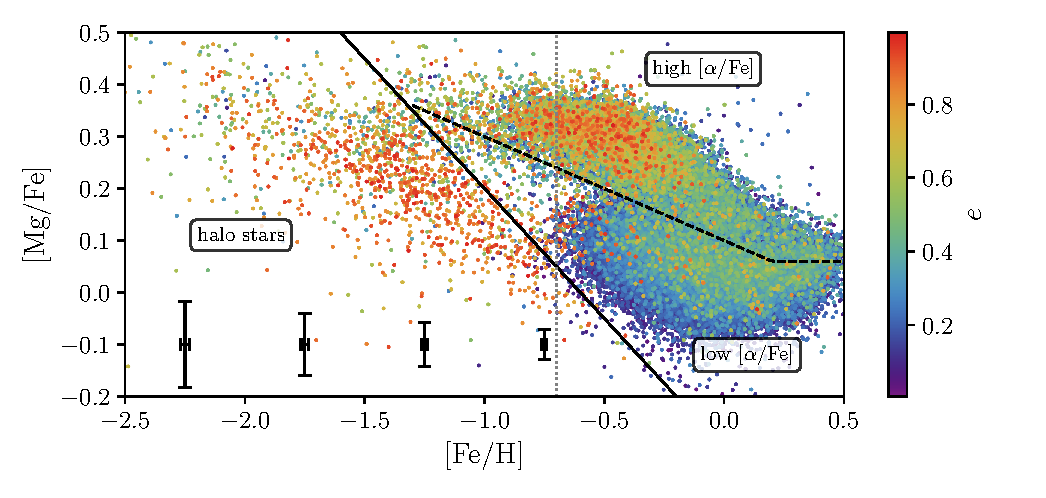
\includegraphics[width=1.0\textwidth]{characterisation.pdf}
\caption[The \mgfe{}-\feh{} plane for APOGEE DR12 stars, coloured by their orbital eccentricity]{\label{fig:characterisation} The \mgfe{}-\feh{} plane in
APOGEE DR14, coloured by orbital eccentricity $e$, as estimated
using the method of \citet{2018arXiv180202592M}. The points are
plotted with the highest $e$ stars overlaying the points at lower
$e$, such that the highest $e$ populations stand out.  Plotted
also are the mean error bars within \feh{} bins of width 0.5 dex
between -2.5 and -0.5 dex. It is clear that a population extends from
(\feh{},\mgfe{}) $\sim$  (-2.0, 0.3) to $\sim$ (-1.0, 0.1) that
appears to consist mainly of stars on highly eccentric orbits, with
a distinct element abundance pattern to that of the Galactic disc
(at \feh{}$>-0.7$). The dotted gray line reflects the cut in \feh{}
which is imposed to perform the $k$-means analysis.}
\end{figure*}


 This finding motivates an attempt at identification
of sub-structure in chemo-kinematic space in an objective and
data-driven fashion, so as to avoid ``cherry-picking'' arbitrary
selection limits in various parameters.  In this way I hope to
characterise the populations within the halo star locus by sub-dividing
its members into meaningful groups.  I use the \texttt{scikit-learn}
$k$-means clustering algorithm \citep{scikit-learn} in the space
of \feh{}, \mgfe{}, \alfe{}, \nife{} and eccentricity $e$.  The
choice of these parameters is guided by the fact that, on one hand,
these elements fall into the main groups: $\alpha$, odd-z and Fe
peak elements, respectively, and on the other hand it appears, at
least from Figure \ref{fig:characterisation}, that eccentricity is
a useful discriminator between disc and halo populations.  I limit
the maximum \feh{} to --0.7, to minimise contamination by disc
stars, finding that high $e$ stars in the low \afe{} disc locus at
higher \feh{} are in no way chemically similar to those in the ``halo
stars'' population and can be confidently disregarded. I set the
assumed number of clusters at $k= 4$, to anticipate the expected
separation of the high and low \afe{} disc, and then to allow for
subdivision of the halo population into any potentially meaningful
groups.  I find that the algorithm groups the high and low \afe{}
disc stars separately, and finds two clear groups in the lower
\feh{} space.  Setting $k>4$ subdivides the lower \feh{} groups in
an unstable manner, while $k=4$ provides very good stability over
many iterations of the algorithm. I also test the algorithm at $k
< 4$, finding that the stability is decreased also at lower $k$.
If the ``halo stars'' group from Figure \ref{fig:characterisation}
is isolated, using $k=2$ clustering can still recover the two groups
found when clustering the whole data set. I retain the full data-set
and use the $k=4$ clustering to avoid resorting to an arbitrary
selection of the division between halo and disc stars, which occupy a similar space in \feh{}. Re-scaling
the data and re-running the clustering algorithm leads to
negligible differences in the results. It is worth noting that
both halo populations have lower abundance ratios than thick disc
stars (in the region where they overlap in [Fe/H]) for C+N, Si, K,
Ca, and possibly also Mn.

I show the eccentricity distributions of the $k$-means groups in
Figure \ref{fig:eccdist}. The high and low~\afe{} disc groups are
combined into a single group in this plot, as these stars
are not of interest to this work, except as a comparison sample.
The halo stars naturally split up into two groups, one
with intermediate eccentricities, peaking at $e \sim 0.5$, and
another with very high eccentricities, peaking at $e \sim
0.9$. The lower $e$ population distribution is fairly broad whereas
the high~$e$ population is very strongly peaked toward the highest
$e$ values (with some small skew to low $e$). The high and low~$e$
groups contain 679 and 318 stars, respectively. I also show the
$k$-means groups in \alfe{}-\mgfe{} space in Figure \ref{fig:mgal}.
This abundance plane was shown by \citet{2015MNRAS.453..758H} to
discriminate well between accreted and in-situ stellar populations
in the Milky Way, with the former occupying the low \alfe{}, low
\mgfe{} region of the plot.  Indeed, I find that the halo population
separates out from the disc population very clearly in this plane,
being characterised by lower Al and Mg abundances.  Moreover, while
there is considerable overlap between high and low~$e$ populations
in this abundance plane, the high~$e$ group occupies a lower \mgfe{}
locus, on average, than the low~$e$ group. 


\begin{figure}
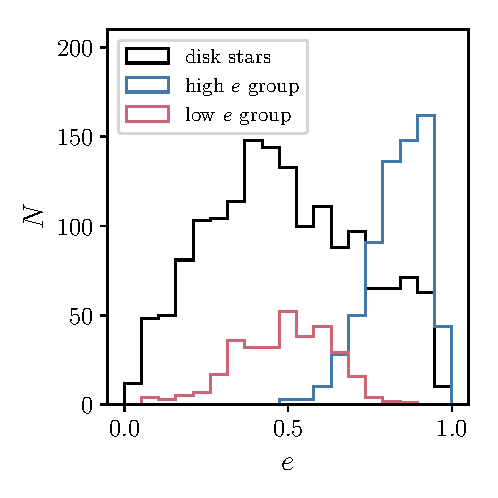
\includegraphics[width=0.5\columnwidth]{eccdist_kmeansselect.pdf}
\caption[Eccentricity distributions of stars in the $k$-means groups identified in Section \ref{highe}]{\label{fig:eccdist} Eccentricity distributions of stars
in three groups identified by performing a $k$-means detection of
structure in the eccentricity-\feh{}-\mgfe{}-\alfe{}-\nife{} space.
The $k$-means algorithm cleanly separates the accreted halo component
into two groups, one characterised by low eccentricities (in red),
and the other with a peak at very high $e$ (in blue).  The
stars assigned to the disc (with \feh{} $< -0.7$) are shown in black, as a
comparison sample. }
\end{figure}


\begin{figure}
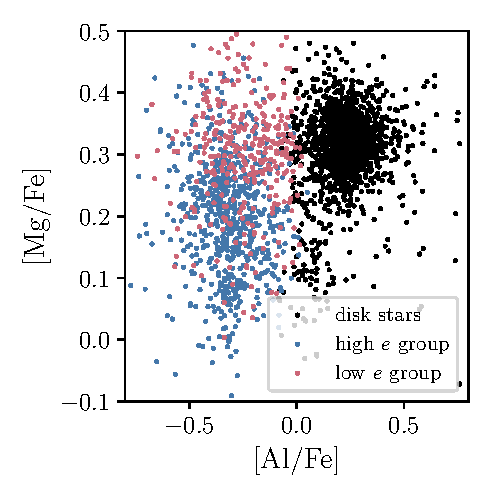
\includegraphics[width=0.5\columnwidth]{mgal_kmeansselect.pdf}
\caption[The \mgfe{}-\alfe{} distribution of the $k$-means groups identified in Section \ref{highe}]{\label{fig:mgal}  Distribution of the stars in the different
$k$-means groups in the \mgfe{}-\alfe{} plane.  High $e$ stars
occupy preferentially the low \alfe{}, low \mgfe{} region of the plot, a locus which was identified
in \citet{2015MNRAS.453..758H} as being common to accreted halo populations. Low~$e$ group stars
tend to be more distributed at higher \mgfe{} and slightly higher
\alfe{}. Disc stars (in black) are enhanced in Al and, to a lesser
extent, Mg, relative to the high and low~$e$ groups.}
\end{figure}



In conclusion, the results above show that once APOGEE chemical
compositions are combined with kinematics inferred from Gaia DR2
proper motions, $\sim 2/3$ of the stars in the accreted halo
population identified in previous studies are characterised by
highly eccentric orbits.  In the following sections I examine
the properties of this population in both orbital and element
abundance space compared to those of their low~$e$ counterparts.

\subsection{Chemical Compositions}

\subsubsection{Metallicity Distributions} \label{sec:mdfs}

In this section, I examine more closely the chemical compositions
of the halo stellar populations, keeping track of the differences
between the high and low~$e$ groups. I begin by examining the
metallicity distribution function (MDF) of these populations.  The
{\it raw} MDFs are displayed in Figure \ref{fig:mdfs}, and are {\it
not} corrected for the APOGEE selection function. Correction for
selection function effects cannot be performed for the full sample
of stars studied here, as many of the sample stars belong to magnitude
bins on plates where observations were incomplete in DR14 and so
are not part of the statistical sample \citep[see][for details on
the selection function of APOGEE and the targeting strategy,
respectively]{2014ApJ...790..127B,2013AJ....146...81Z}. 
As a result, a selection function correction would leave a
much smaller sample, resulting in more uncertain MDFs, particularly
in the case of the smaller low~$e$ population sample.  I nevertheless
compared the lower $N$, corrected and raw MDFs for the larger
high~$e$ sample, which is statistically more robust, and found that
they were in good overall agreement, with similar peak position and
width.  Moreover, it
is reasonable to assume that relative differences between the MDFs
of the high and low~$e$ populations are also not affected significantly
by selection biases from the targeting strategy, and that any
differences in the MDFs are likely to be real. Therefore, we can
confidently compare the MDFs of the high and low~$e$ populations,
at least to first order.  It should be noted here that \feh{} is
included in the $k$-means analysis, and so these MDFs are reflective
of the metallicities of the groups as defined by that procedure.

With the above caveats in mind, Figure \ref{fig:mdfs}
demonstrates that the MDF of the high~$e$ population peaks at \feh{}$\sim$--1.3
and has a width of approximately 0.6 dex (FWHM), with a tail towards
the metal-poor end, resembling the MDF of a classical closed-box
model.  The high-$e$ MDF is in fact qualitatively similar to those of
relatively massive dwarf galaxies in the Local Group
\citep[e.g.][]{2015AJ....149..198R}, particularly those of the Small Magellanic Cloud \citep[SMC,][]{2014MNRAS.442.1680D}
and Leo I \citep{2013ApJ...779..102K}. This is an interesting result
given that \citet{2018ApJ...852...49H} showed that their LMg
population (of which the high~$e$ stars are a sub-group) had a star
formation history similar to that of massive dwarfs such
as the LMC prior to its accretion which, if accreted, would have likely been
around present day SMC mass \citep[$\sim 3\times 10^{8}
\mathrm{M_{\odot}}$, e.g.][]{2004ApJ...604..176S,2018MNRAS.478.5017R}
at the time that the LMg population was accreted
\citep{2009IAUS..256...81V,2018arXiv180606038H}.

It is also instructive to compare the MDFs of the high and low~$e$
populations.  The most striking difference is that the MDF of the
low~$e$ population has no strong peak, but rather two smaller (likely
significant) peaks at lower metallicities.  The sharp edge at
\feh{}=--0.7 is due to the \feh{} limit adopted in the $k$-means
grouping, and the smaller peak of the low~$e$ population at
\feh{}$>$--1.0 is likely due to contamination from the disc.  Interestingly,
the two peaks towards the lower metallicity end happen at similar
metallicities to those previously assigned to the inner and outer
halo populations
\citep[e.g.][]{2007Natur.450.1020C,2014A&A...568A...7A,2015A&A...577A..81F}.
Most importantly, the MDFs of the high and low~$e$ populations are
strikingly different and, as argued above, this difference
is almost certainly insensitive to target selection effects, which
then strongly suggests that the two populations have different
origins.

It is not entirely clear how the difference in shape between the
MDFs of the high and low~$e$ populations can be understood in terms of the halo accretion history.  While the MDF of the high~$e$
population lends support to the notion that those stars were injected
into the halo as part of one major accretion event, it is
hard to draw any strong conclusion regarding the low~$e$ population.

\begin{figure}
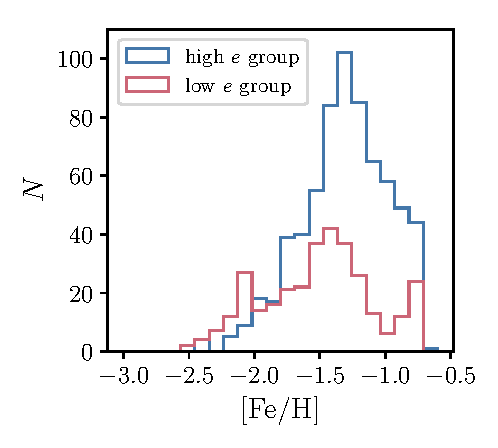
\includegraphics[width=0.6\columnwidth]{MDFhist_kmeansselect.pdf}
\caption[Metallicity distribution functions of the $k$-means groups identified in Section \ref{highe}]{\label{fig:mdfs} Raw metallicity distribution functions
of the high and low~$e$ populations.  Unlike their low~$e$ counterparts,
the high $e$ population shows a strong peak at about \feh{}$\sim
-1.3$, resembling MDFs of Local Group dwarfs. The low~$e$ group
shows peaks at both \feh{} $\sim -2.1$ and $\sim -1.4$, and stars
piled up at the imposed upper \feh{} limit at \feh{} $= -0.7$.
}
\end{figure}

\subsubsection{Abundance Ratios}
\label{sec:abundances}
 In this section, I inspect abundance ratios of the high and
low~$e$ groups, to gain further insights into the origins of these
two populations.  Figure \ref{fig:mgalni} displays the run of
[Mg/Fe], [Al/Fe], and [Ni/Fe] as a function of \feh{}.  For each
element I demonstrate the running median and interquartile range of
$\mathrm{[X/Fe]}$ as a function of \feh{}. I calculate
the median abundance in bins of 50 stars sorted by increasing \feh{},
which is shown by the red and blue coloured bands for the high and
low~$e$ populations, respectively.

\begin{figure}
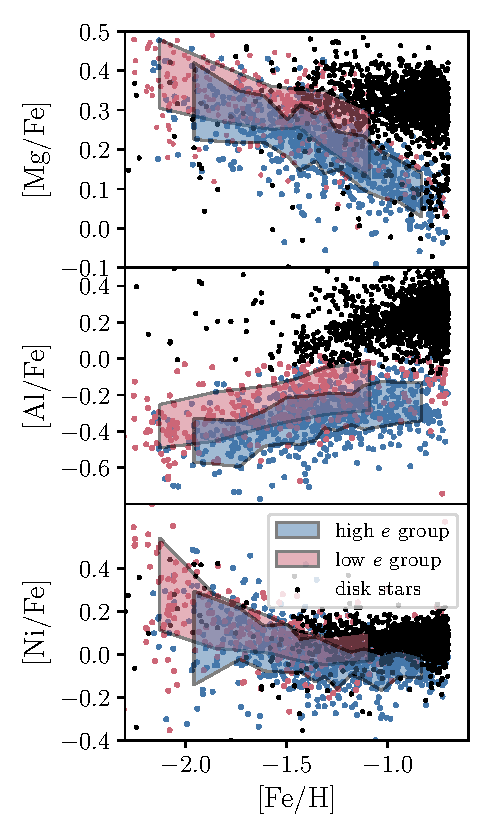
\includegraphics[width=0.5\columnwidth]{mgalni_kmeansselect.pdf}
\caption[\mgfe{}, \alfe{} and \nife{} abundance ratios of the low and high $e$ $k$-means groups, as a function of \feh{}]{\label{fig:mgalni} Abundance ratios for the $k$-means
groups as a function of [Fe/H]. These elements are good representations
of $\alpha$, odd-$Z$ and Fe peak elements that are measured by
APOGEE. The coloured bands show the interquartile range in bins of
50 stars sorted in increasing \feh{}. The high and low~$e$ populations
are characterised by lower Mg and Al than the high-$\alpha$ stars.
The bottom panel shows that the high~$e$ group has slightly lower
[Ni/Fe] than the high-$\alpha$ population, whereas the low~$e$ group
is essentially consistent with the high-$\alpha$ population in
[Ni/Fe]. In all cases, the high~$e$ group median is slightly lower
than the low~$e$ group at fixed \feh{}. The slightly higher \feh{}
of the high~$e$ population is also evident here.  Again, both groups
are depleted in all these elements relative to the disc stars at
that \feh{}.}
\end{figure}

The top panel of Figure \ref{fig:mgalni} shows that, in general, \mgfe{} decreases with \feh{}
and both the high and low~$e$ populations have \mgfe{} lower than
that of the high-$\alpha$ disc stars at same \feh{}, in the metallicity
interval where those populations overlap
($\mathrm{-1.5\simless[Fe/H]\simless-0.5}$) -- as previously discussed
by \cite{2018ApJ...852...49H} and \citet{2018ApJ...852...50F}.
Moreover, the high and low~$e$ populations occupy slightly separated
sequences, such that the former has lower \mgfe{} at fixed \feh{}.
It appears from the simple running median that the high~$e$ population
exhibits a change in slope of \mgfe{} against \feh{}, at \feh{}$\sim-1.3$,
whilst there is only slight evidence change of slope in the lower
edge of the low~$e$ relation.  In order to test this further, and
to determine more rigorously the location of the change in slope,
I use a Bayesian inference to determine a generative model for the
\mgfe{}-\feh{} distribution of both populations. The full procedure
is outlined in Appendix \ref{sec:appA}, the basic principle being
that I fit a piecewise-linear model to the data of the form:

\begin{equation}
\label{eq:pwlin}
\mathrm{[Mg/Fe]}(\mathrm{[Fe/H]}) =
  \begin{cases}
    m_{1}\mathrm{[Fe/H]} + b_1  &  \quad \mathrm{[Fe/H]} < \mathrm{[Fe/H]}_0\\
    m_{2}\mathrm{[Fe/H]} + b_2  &  \quad \mathrm{[Fe/H]} > \mathrm{[Fe/H]}_0
  \end{cases}
\end{equation}

\noindent where $m_{[1,2]}$ and $b_{[1,2]}$ are the slope and
$y$-intercept either side of the break, which is positioned at
$\mathrm{[Fe/H]}=\mathrm{[Fe/H]}_0$. The fitting procedure accounts
for the error on both \mgfe{} and \feh{}, allowing a proper assessment
of the significance of any fitted breaks. If there is no break in
the range of \mgfe{} and \feh{} considered, the data are fit by a
simple linear relation, as the break is pushed to the edge of the
\feh{} range.

I show the models fitted to the high and low~$e$ groups in Figure
\ref{fig:mgknee}. The data for each group are shown as black
points, and the best fit and 95$\%$ confidence interval are given
by the line and coloured bands in each panel. The best fit high~$e$ group
model (in the top panel) has a change of slope, indicated by the dashed crosshair, positioned at
\feh{}$=-1.31^{+0.03}_{-0.06}$ and \mgfe{}$=0.22^{+0.01}_{-0.08}$.
The  slope to the metal-poor side of the break is found to
be $-0.15\pm{0.01}$, and is roughly consistent with the slope before
the break in the high \mgfe{} disc star sequence \citep[e.g. that
seen in][]{2015ApJ...808..132H}. A similar metal-poor end slope 
is also present in the work of \citet{2018ApJ...852...50F},
who used APOGEE DR13 data to determine also that a change of slope
is present in low \mgfe{} stars, located at \feh{}$\sim-1.0$ dex,
in rough agreement with that found here. At \feh{}$>\mathrm{[Fe/H]}_0$,
the slope steepens to become $-0.26\pm{0.01}$. The low~$e$ population
is well fit in this range of \feh{} by a simple linear relation
with a slope equal to $-0.14\pm{0.01}$, with no significant break
found. As it is likely that at least some of the stars at the highest
\feh{}, and at high \mgfe{} in this population are high \afe{} disc
contaminants, I also perform the same fit using only stars at \feh{}~$<-1.$
dex, and still find no evidence of a break at the same position as
that found in the high~$e$ group. Fitting only low~$e$ stars with
\feh{}~$>-1.1$ dex, we find that the best fit is a single linear
relation with a slope equal to that found when using the whole
low~$e$ group.

\begin{figure}
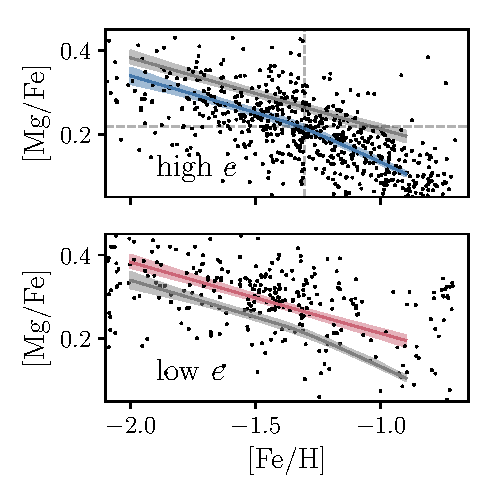
\includegraphics[width=0.5\columnwidth]{mgfe_kneefit_separated.pdf}
\caption[Best fit models for the \mgfe{} as a function of \feh{} for the low and high $e$ groups, showing the change of slope in \mgfe{}-\feh{} for the high $e$ population]{\label{fig:mgknee} Best fit models for \mgfe{} as a
function of \feh{} for the high and low~$e$ $k$-means groups (shown
top and bottom, respectively). The best fit model is shown by the
blue and red lines, with the 95$\%$ confidence interval marked by
the banded blue and red regions either side of this line (the fit
for the other group is shown in each panel for reference). The raw
data are shown by the black scatter points. The high~$e$ group is
well-fit by a model with a break at \feh{}$=-1.31^{+0.03}_{-0.06}$
and \mgfe{}$=0.22^{+0.01}_{-0.08}$, as indicated by the dashed
crosshair. The low~$e$ group is better fit by a single linear
relation in the same range of \feh{}. The position of the models
also demonstrates the slightly higher \mgfe{} of the low~$e$ group.}
\end{figure}


\begin{figure*}
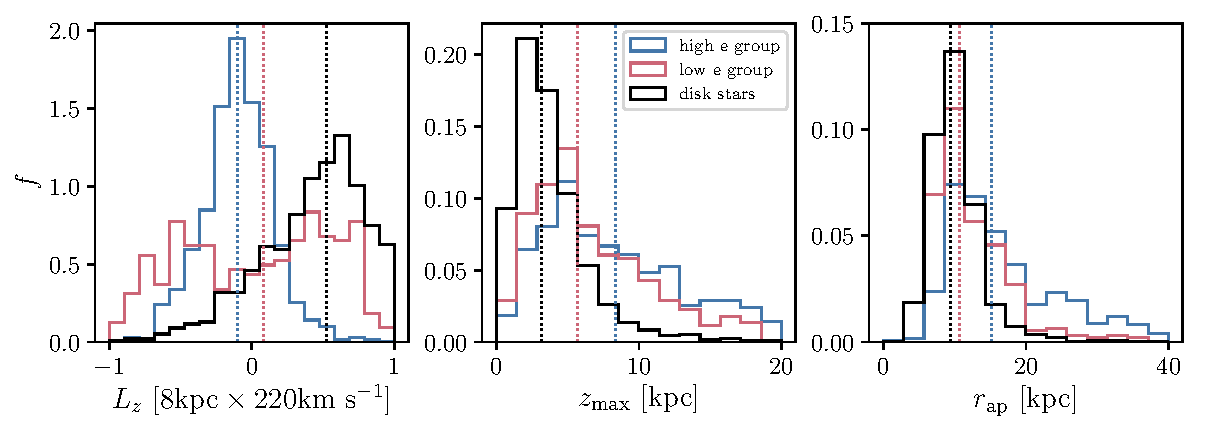
\includegraphics[width=\textwidth]{Lz_zmax_rap_histograms.pdf} 
\caption[Angular momentum, $z_\mathrm{max}$ and $r_\mathrm{ap}$ distributions of the $k$-means groups]{\label{fig:kinematics} Kinematics of the k-means-selected
stars from Figure \ref{fig:characterisation}. The distribution
of azimuthal angular momentum $L_z$ (\emph{left}), maximum vertical
excursion from the disc plane $z_\mathrm{max}$ (\emph{centre}), and
the spherical apocentre radius of orbits $r_\mathrm{ap}$ (\emph{right}),
are shown for the high and low \afe{} disc (red and yellow, respectively)
and the accreted halo population (blue). The halo stars clearly
occupy a very different orbital distribution, having low $L_z$, and
distributions of $z_\mathrm{max}$ and $r_\mathrm{ap}$ that extend
to very large distances. The median $L_z$ is slightly negative,
while the median $z_\mathrm{max}$ and $r_\mathrm{ap}$ are $\sim10$
and $\sim 20$ kpc, respectively. All histograms are normalised such
that the integrated probability under \emph{each} group is equal to
unity.}
\end{figure*}


This change of slope in the \mgfe{}-\feh{} relation of the high~$e$
population offers important clues on the nature of this stellar
population. This feature is most commonly interpreted as being due
to the onset of Fe enrichment by SNe Ia.  The \feh{} at which the
change of slope occurs is primarily related to the star formation
efficiency \citep[e.g.][]{2017ApJ...837..183W}, and additionally
depends on the gas inflow and outflow rates of its parent galaxy.
It follows that it should also be a function of the mass of the
parent galaxy, which regulates gas density and gas inflow/outflow.
Data for stellar samples from Local Group dwarf galaxies indicate
the presence of this same change of slope on the Mg-Fe plane, and
it is suggested that the \feh{} at which it occurs is higher in
galaxies with larger luminosity, and presumably higher stellar mass
\citep[see,e.g.][]{2009ARA&A..47..371T}.  Given the \feh{} at which
data for Local Group dwarf galaxies show a change of slope
\citep[see,e.g.][]{2009ARA&A..47..371T}, I estimate that the mass
of the progenitor of this high~$e$ population was somewhere between
$10^{8}$ and $10^{9} M_\odot$. This rough mass estimate is in good
agreement with that inferred from arguments based on the MDF of the
high~$e$ population in Section~\ref{sec:mdfs}.  It moreover places
the mass involved in this accretion event within the range of the
total stellar mass of the Galactic halo \citep[$\sim 4 - 7 \times
10^8\ \mathrm{M_{\odot}}$] {2016ARA&A..54..529B} which presents a concrete argument against
the high~$e$ population belonging to more than one major accretion
event, as multiple accretions at this mass would exceed this mass
limit. In contrast, the lack of a clear change of slope in the
distribution of the low~$e$ stars on the Mg-Fe plane argues
strongly for this group being in fact some mix of stellar populations
with various origins, including stars accreted in different smaller
events, stars formed \emph{in situ}, ejected members of the disc,
 and contamination by members of the low-$e$ tail of the
high~$e$ group.

The middle panel of Figure~\ref{fig:mgalni} shows the run of \alfe{}
with \feh{}.  As pointed out by \citet{2018ApJ...852...49H},
their LMg (and thus also the high~$e$) population is characterised
by much lower \alfe{} than the disc populations at same \feh{}.  In
fact, \alfe{} in those populations is comparable to that
of stars in the Sagittarius dwarf spheroidal \citep{2017ApJ...845..162H}.
 In addition, the high and low~$e$ populations occupy
separate loci in \alfe{}-\feh{} space, with the high $e$
population showing lower \alfe{}.  For both populations \alfe{}
increases with \feh{}. As an odd-$Z$ element, Al is an important
component in the explosive ejecta of massive stars, synthesised in
their carbon and nitrogen hydrostatic burning phases. It is also a
product of Asymptotic Giant Branch (AGB) stellar nucleosynthesis,
particularly at \feh{}$> -0.2$ dex \citep[see,
e.g.][]{2016arXiv160408613A}. Importantly, it is known that odd-$Z$
element yields should be metallicity dependent to some extent due
to their dependence on a high neutron surplus
\citep[e.g.][]{1996snih.book.....A}. This fact may explain the
slight correlation observed between \alfe{} and \feh{} in each group
and also in the disc populations.  The depletion in \alfe{} relative
to the MW disc in both halo groups has no
straightforward explanation, and I speculate that it may indicate
that AGB stars contributed more importantly to the enrichment of
MW disc ISM.


While the trend in Ni abundances as a function of \feh{} of the
high~$e$ group appears to be roughly similar to that of the low~$e$
group, it is noteworthy that the trend is negative in both groups,
such that \nife{} decreases with increasing \feh{}.  Similarly to
the other elements, Ni is slightly depleted in the high~$e$ group
relative to the low~$e$ group, but this depletion is very small.
At fixed \feh{}, the high~$e$ group has a lower \nife{} than the
disc stars, whereas the low~$e$ group is nearly consistent
with them. 

I also studied the other $\alpha$, odd-$Z$ and Fe peak elements
available in APOGEE. These trends appear to be consistent between
most of the elements, depending on their source (i.e. all $\alpha$ elements show similar trends). It is noteworthy that in almost all elements,
the low~$e$ group appears to show slightly higher abundance ratios
than the high~$e$ group, at fixed \feh{}, which may be difficult
to explain by invoking lower mass accretion events, unless the star
formation in these stellar populations was very short and intense.
The discussion of the EAGLE simulations in Section \ref{eagle} sheds
some light on this matter.  


\subsection{Kinematics}

Figure \ref{fig:kinematics} shows the distribution of the $k$-means
groups in (from left to right) azimuthal angular-momentum $L_z$
(equivalent to the azimuthal action $J_\phi$), the maximum vertical
excursion of orbits above the midplane $z_\mathrm{max}$, and the
apocentric radius $r_\mathrm{ap}$, which is the maximum orbital
distance from the Galactic centre. The median value of each
distribution is shown by the coloured vertical dashed line. 

It is clear from these Figures that the halo groups (again,
shown in red and blue) have a very different orbit distribution
than the disc stars (in black).  The latter are characterised by
highly prograde orbits with relatively low vertical excursions.  In
turn, the two accreted halo populations differ substantially,
particularly in terms of their $L_z$ distributions. The high~$e$
stars all have extremely low angular momentum, such that many of
the stars in this population have negative $L_z$. The lower $e$
population has a large spread in $L_z$, such that many stars are
on prograde orbits while others have negative $L_z$, thus moving
on retrograde orbits. The lack of a distinct single peak in $L_z$
space for the low~$e$ group may indicate again that this group is
in fact a superposition of populations with different origins,
including the debris of accreted satellites with lower masses, whereas
the single, clear peak in $L_z$ for the high~$e$ group supports the
notion that this population is mainly the debris of a single
satellite. The median value of $L_z$ for the high~$e$ stars is $-176
\mathrm{\ km\ s^{-1}\ kpc}$.  A slightly retrograde motion for stars
in the halo at roughly these eccentricities was noted by
\citet{2018arXiv180606038H} and, as they suggest, could be either
an effect of the assumption of the solar motion (which is likely
subject to some systematic uncertainties), or could be a true feature
of this population, which further supports its origin in a single
accreted satellite. I find that a slight retrograde motion of the
high~$e$ stars is present when assuming either the
\citet{2010MNRAS.403.1829S} or the \citet{2005ApJ...629..268H} solar
motion measurements, which differ markedly.

The $z_\mathrm{max}$ distribution shows that the stars belonging
to the high and low~$e$ populations are on orbits that take them
very far above the midplane of the Galaxy, extending to $z_\mathrm{max}>10$
kpc, as expected for halo stars. The median $z_\mathrm{max}$ of the
high~$e$ population is higher than the other two populations, at
8.8 kpc. Similarly, the apocentre radii of these stars extend to
very large distances from the Galactic centre with a median
$r_\mathrm{ap} = 15.1$ kpc.  There appears to be a secondary peak
in the distribution at $r_\mathrm{ap} >\sim25$ kpc, which is roughly
consistent with the ``apocenter pile up'' suggested by
\citet{2018arXiv180510288D}.  Considering that roughly 2/3
of the stars in the halo population are on highly eccentric orbits
($e > 0.8$) which are strongly out of the disc plane ($z_\mathrm{max}
> 10$ kpc), and have a median apocentre radius which is comparable
to that of the accreted halo population analysed by
\citet{2018arXiv180510288D}, it seems reasonable to conclude that
the high~$e$ stars are part of that population.

Further insights into the nature of the high and low~$e$ stellar
populations can be gained by inspection of Figure \ref{fig:polar},
where they are displayed together with disc populations on three
cylindric coordinate velocity planes.  The left panel shows
the $v_R-v_\phi$ plane, where the high $e$ population has a wide
spread in $v_R$ and a much narrower distribution in $v_\phi$.  This
is the same locus as that of the population identified by \citet[][their
Figure 2]{2018MNRAS.478..611B}.  The low $e$ group, on the other
hand, has a clearly bimodal distribution, with two concentrations
above and below the high $e$ population.  The concentration at
higher $v_\phi$ shows {\it prograde} rotation, overlapping well
with the disc population.  The grouping at lower $v_\phi$ is markedly
{\it retrograde}.  These two sub-populations are also clearly seen
on the right panel, where one can notice that their distributions
in $v_z$ are very similar.  The presence of such obvious structure
in velocity space calls for a closer scrutiny of those two
sub-populations in chemical composition space.

Upon comparison of the low~$e$ prograde and retrograde populations in MDF,
\mgfe{}-\feh{}, \alfe{}-\feh{}, and \nife{}-\feh{} spaces and found them to be indistinguishable from each other, but still clearly
distinct from the high~$e$ population in all diagnostic plots.  It
is likely that there is some degree of inter-contamination between
all these groups, so that the left panel of Figure \ref{fig:polar}
suggests strongly that the prograde population can be contributed
entirely or in part by the disc.  This is also suggested by the
presence of a secondary peak at the high \feh{} end of the low $e$
MDF (see Figure \ref{fig:mdfs}) which is dominated by prograde
stars.  However, the prograde population is
chemically indistinguishable from its retrograde counterpart, which
is unlikely to be contributed by the disc.  I tested this further
by re-fitting the relation between \mgfe{} and \feh{} for the
separated prograde and retrograde components, using the procedure
described in Appendix \ref{sec:appA}. We find that in both cases,
the best fit relation matches that found for the combined population
within the uncertainties, and furthermore, find no evidence of a
change in slope in \emph{either} population.  Without further diagnostics
with which to make a call on the nature of the distinct low $e$
populations, I summarise the situation by concluding that it is
likely to be a mix of stars contributed by contaminants
from the high~$e$ population, smaller accretion events, heated
disc stars, and potentially stars formed {\it in situ} in the halo.

\begin{figure*} 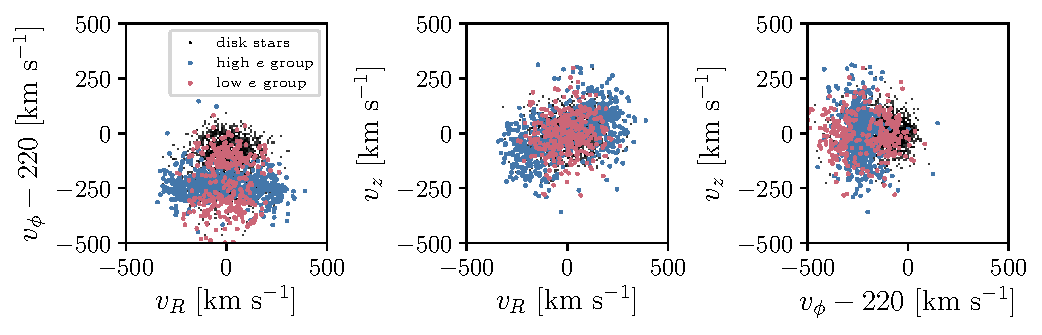
\includegraphics[width=\textwidth]{kmeans_kinematics.pdf}
\caption[The distribution of disc and accreted halo
populations in spherical polar coordinate planes, coloured by membership in the low and high $e$ groups]{\label{fig:polar} Distribution of disc and accreted halo
populations in spherical polar coordinate planes.  On the left
panel, the high $e$ population occupies the same locus in $v_R-v_\phi$
space (left panel) as the population identified by
\citet{2018MNRAS.478..611B}.  The low $e$ population splits into
two populations according to $v_\phi$, with one prograde and one
retrograde component, suggesting that this population may in fact
be from a mix of disc contaminants and debris from smaller satellites.
} \end{figure*}


\section{Accreted Stellar Populations in EAGLE} \label{eagle}

I have demonstrated that the halo stellar populations in the
combined APOGEE and Gaia DR2 samples have MDFs and abundance
patterns that are similar to those of dwarf galaxies in the Local
Group. Furthermore, I have shown that this population contains
two distinct sub-groups, with different chemical and kinematic
characteristics. One of these groups is characterised by highly
eccentric and slightly retrograde orbits, thus sharing similar
properties with stellar populations ascribed to a major accretion
event in the distant past.  In this Section I examine the predictions
of numerical simulations, drawing parallels with the observations
to gain insights into the nature of this accreted halo
population.  The questions I intend to address with this exercise
are the following: is the high~$e$ population the result of a single
relatively massive accretion event, as claimed by other groups?  Do
the simulations provide insight into the nature of the low~$e$
population? Is it composed of a collection of small accretion events,
or is it predominantly formed {\it in situ}? 

The EAGLE simulations are a useful tool to address these questions,
as they provide a  cosmologically motivated history of satellite
accretion for Milky Way-like galaxies, simulated self-consistently
in a cosmological context.  Therefore,  we expect the  $z=0$ dynamical
state of accreted systems around Milky Way analogues in the simulations
to be a good approximation to the observations in the Milky Way
halo. In order to attempt to shed light on the problem using EAGLE, I track star particles formed in galaxies which merged onto disc galaxies that eventually reach a
virial mass roughly equal to that of the Milky Way ($\sim 10^{12}
\mathrm{M_{\odot}}$). At $z=0$, I measure the orbital eccentricity
$e$ of the star particles resulting from all well-resolved accretion
events (i.e., those having $>20$ star particles) of 
systems with stellar mass $M_*$, occuring at redshift $z_\mathrm{merge}$.

\begin{figure}
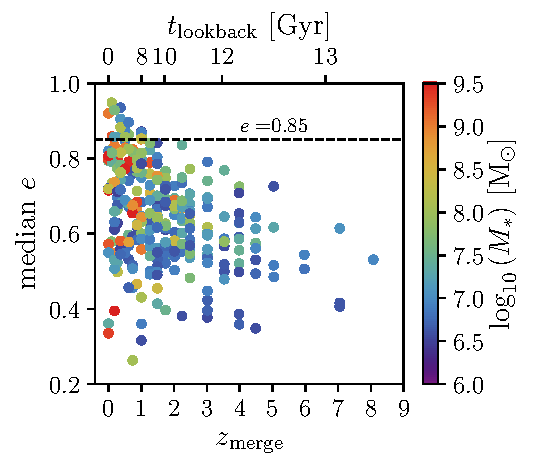
\includegraphics[width=0.5\columnwidth]{L025N752_RECAL_zmerge_mediane_npart20.pdf}
\caption[Median eccentricity of satellites accreted onto Milky Way mass haloes as a function of their merger time, in the Recal-L025N0752 EAGLE simulation]{\label{fig:eagle}Merger redshift and lookback
time ($z_\mathrm{merge}$ and $t_{\mathrm{lookback}})$ of 296
satellite galaxies accreted onto 22 Milky Way mass haloes in EAGLE
against the median eccentricity $e$ of their stellar debris at
$z=0$. The points are coloured by the stellar mass of the accreted
galaxies at the time of the merger, $M_*$. The larger points denote
those galaxies which have $N > 100$ star particles in EAGLE, whereas
the smaller points are those galaxies with $20 < N < 100$ particles.
Open points indicate satellites accreted onto galaxies which do not
have a clear disk component at $z=0$ (defined as described in Section
\ref{eagledata}). The dashed horizontal line indicates $e = 0.85$,
which is the median eccentricity of the high~$e$ group characterised
in Section \ref{highe}. Only the latest merged haloes have debris
at the highest and lowest $e$, whereas early mergers tend to occupy
intermediate $e$. The most massive mergers also occur later, with
early mergers dominated by low mass haloes.}
\end{figure}

In Figure \ref{fig:eagle},
I show the median $e$ of star particle orbits against
$z_\mathrm{merge}$ for accreted satellites onto the 22
simulated galaxies with Milky Way-like virial mass ($\sim 10^{12}
\mathrm{M_{\odot}}$) in the EAGLE L025N752-Recal simulation.
Each point is coloured according to the stellar mass reached
by the progenitor population prior to merging onto the main
progenitor. The median eccentricity of the high~$e$ group
found in the Milky Way halo (discussed in Section \ref{highe}) is indicated as a dashed horizontal line. To
ensure proper resolution of the orbital properties of the stellar
component of the accreted satellites, I only show galaxies with
20 or more star particles, amounting to a total of 296 accreted
satellites. The satellites with $20 < N < 100$ particles are shown
by small symbols, whereas large symbols are adopted
for satellites with $N > 100$.  Satellites accreted onto
galaxies that are not dominated by a disk component (as discussed
in Section \ref{eagledata}), are plotted as open symbols.

There is a striking trend of median $e$ with $z_{\mathrm{merge}}$
in Figure \ref{fig:eagle}. The maximum median $e$ decreases with
lookback time, creating an upper envelope to the distribution of
the data.  As a result, $z=0$ stellar particles resulting from the
earliest accretions typically have median $e\sim0.5$, whereas the
most recently accreted satellites span a wide range of median
$e$, from $\sim 0.3$ up to $> 0.9$.  As I will discuss below, this means
that early accreted satellites were accreted onto intermediate to
low $e$ orbits.  Most importantly, this result implies that 
an accreted satellite whose stars at $z=0$ are on very radial orbits is
unlikely to have been accreted before $z\sim1.5$. I
verify that this trend is not due to numerical noise in Appendix
\ref{sec:appB} by demonstrating that the same trend is realised
in a larger volume simulation (at lower resolution), with a far
larger sample of accreted satellites (see Figure \ref{fig:l50}). I
discuss the implications of this finding for the formation of the
Milky Way thick disc, as suggested by \citet{2018arXiv180606038H},
in Section \ref{finale}.

As expected from hierarchical galaxy mass growth in a
standard $\Lambda$-CDM universe, it can be seen in Figure \ref{fig:eagle}
that, at the highest redshifts, merged satellite galaxies are
relatively low mass.  Conversely, the most massive galaxies
were accreted more recently.  Almost all accretion of stellar systems
with $M_* \gtrsim 10^9 M_\odot$ occurs at $z \lesssim 1$.
This is mainly due to the time taken for satellites to build up
their stellar mass. The fact that the satellite debris with the
highest median $e$ must have been accreted late also means that
these satellites are likely to be high mass. I find that the median
mass of accreted satellites with median $e>0.85$ is $4.1\times
10^{8}\ \mathrm{M_{\odot}}$, with a minimum mass of $0.77 \times
10^{8}\ \mathrm{M_{\odot}}$. The median accretion time of high $e$
debris is $z \sim 0.6$. This suggests that the high~$e$ Milky Way
halo population we identify is likely to have had  $M_* \gtrsim
10^{8}\ \mathrm{M_{\odot}}$ and have been accreted after $z\sim
1.5$.  Accretion events such as this are relatively rare in EAGLE,
with only 5 of the 22 ($\sim~23\%$) central galaxies having accreted
any system with $10^8 < M_* < 10^9 \mathrm{M_{\odot}}$ after $z=1.5$
\emph{and} retaining a median $e > 0.8$ at $z=0$.  For two of those
five simulated galaxies, the aggregate of all accreted stellar mass
far exceeds that of the Galactic halo (e.g. by a factor of 2 or
more), leaving only 3 galaxies ($\sim$~14\%) with accretion profiles
resembling that suggested by the observations reported in this
paper.  It is also worth noting that the high~$e$ populations of
the latter three galaxies, although dominated by one massive accretion
event, had significant contributions by accretions of smaller
mass systems.  The latter suggests that it is possible that the
high~$e$ population of the Galactic halo may have contributions by
low mass systems as well. 

Perhaps most importantly, the above discussion indicates that the
accretion event which deposited the high~$e$ Milky Way debris was
quite unusual for a galaxy of its $z=0$ virial mass.  If one further
considers that the Milky Way is currently accreting a similarly
massive galaxy (the Sagittarius Dwarf), and may have accreted
yet another massive system in the distant past (the \emph{Kraken}),
as proposed by \citet{2018MNRAS.tmp.1537K}, our results suggest
that the overall accretion history of the Milky Way has been quite
atypical when compared to the rest of the galaxies of same halo
mass. This is an interesting result in light of the findings reported
by \citet{2018MNRAS.477.5072M}, which suggest that the
distribution of Milky Way disc stars on the \afe{}-\feh{} plane
indicate that it has undergone an unusual accretion history, for
it's stellar mass.  I discuss the implications of that work further
in Section \ref{finale}.

\begin{figure}
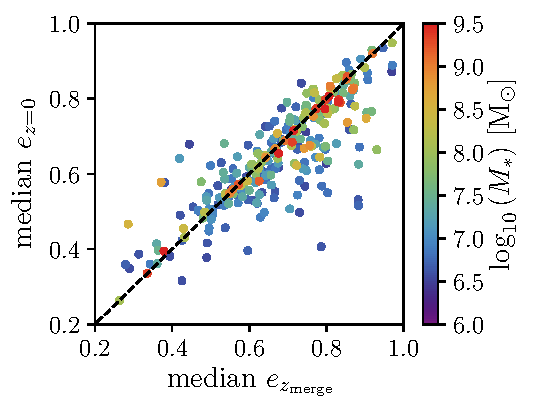
\includegraphics[width=0.6\columnwidth]{L025N752_RECAL_inite_mediane_npart20.pdf}
\caption[The change in median eccentricity between $z=0$ and the time immediately after merger for satellite debris accreted onto Milky Way mass haloes in the Recal-L025N0752 simulation]{\label{fig:echange} Median eccentricities at merger time
$e_{z_\mathrm{merge}}$ against median eccentricity at $z=0$ $e_{z=0}$
for satellites accreted onto Milky Way mass haloes in EAGLE. The
points are coloured by the stellar mass of the accreted galaxies
at the time of the merger, $M_*$.  As in Figure \ref{fig:eagle},
point sizes denote the number of stellar particles in the satellite,
and the open points show satellites accreted onto galaxies with no
clear disk component.  Debris which falls below the dashed unity
line has been circularised following accretion, whereas the debris
above this line has been radialised after accretion. The majority
of debris has a similar $e$ at $z=0$ to the time at which it was
accreted, but a few accreted satellites are circularised/radialised
following accretion. High mass satellite debris has undergone the
least change in median $e$.}
\end{figure}


In Figure \ref{fig:echange}, I show how the eccentricity of satellite
debris changes between the time immediately following the merger and $z=0$. I measure
the initial eccentricity by taking the median eccentricity of the
star particles in the snapshot immediately following that in which
the satellite is identified as being merged onto the main progenitor.
It is clear from this figure that the orbit eccentricities are not
greatly changed following accretion. The median change in eccentricity
is small, at $\sim 4\%$, although a few accreted satellites have
changed their median eccentricity by as much as $\sim 20 \%$. It
is noticeable that the debris whose eccentricity has changed most
is that from lower mass satellites.  As noted previously, these are
the satellites commonly accreted earlier, although I find no
significant trend between $z_\mathrm{merge}$ and the change in
eccentricity, meaning that changes in the median $e$ are not strongly
time dependent.  By the same token, the highest mass satellite
debris are those which have undergone the least change in median
$e$, likely because they were accreted late, when the gravitational
potential of the host dark matter halo is no longer varying
significantly. Furthermore, no satellite accreted at lower $e$
than $\sim 0.7$ has debris that is radialised to higher than $e
\sim 0.8$ by $z=0$. 

The finding that median $e$ changes very little
is important, as it means that the trend between $z_\mathrm{merge}$
and median $e$ at $z=0$ (Figure~\ref{fig:eagle}) is cosmological
in nature, and not due to dynamical effects, substantiating the
idea that high orbit eccentricity is a good indicator of late-time
accretion.  The trend between $z_\mathrm{merge}$ and median $e$ is then
likely to be a product of the changing merger cross-section with cosmic
time, whereby the gravitational potential of the central halo
dictates the maximum impact parameter for a successful accretion
(as opposed to a ``fly-by'').  Galaxies in the early universe are
smaller and less massive, and so approaching satellites must have
a smaller impact parameter to be accreted -- in fact so small
at very high redshift that very eccentric orbits are essentially
impossible to achieve.  For example, under the assumption that at high redshifts ($z\sim$3 to 4), galaxies have small virial radii, $r_\mathrm{vir} \sim
50$~kpc, a high $e$ orbit ($\gtrsim 0.8$) can only be attained by a satellite impacting at $r_{\mathrm{peri}}\lesssim 5.5$~kpc (assuming that the maximum $r_\mathrm{apo}$ is set by the virial radius).  Conversely, for Milky-Way-like centrals with larger virial radii at $z=0$, closer to $r_\mathrm{vir} \sim
250$~kpc, an impacting galaxy can merge anywhere with $r_\mathrm{peri}\simless 28$ kpc for an
orbit with similar eccentricity, meaning that high eccentricity mergers are more likely at lower redshifts. This logic supports the contention
that the high~$e$ group in the Milky Way must have been a relatively
late accretion event.

It is noteworthy that the morphology of the central galaxy does not
seem to impact the trends seen in Figures~\ref{fig:eagle} or
\ref{fig:echange}, since the galaxies without dominant disc components
(open symbols) trace roughly the same locus as  their disc-dominated
counterparts (filled symbols). This is of interest because it
suggests that the galaxy morphology is generally not necessarily
reflective of the galaxy assembly history in terms of merger time,
mass and orbital properties following the merger, at least on the
relatively long timescales shown in these figures. Moreover,
disc and non-disc galaxies have essentially the same mean and
standard deviations around the identity relation in
Figure~\ref{fig:echange} (to within a fraction of a percent).  This
result suggests that the evolving galaxy morphology has little
effect on the orbital evolution of accreted debris once the satellite
is fully unbound.

Regarding the low~$e$ group, the numerical simulations reinforce
the notion that it may be contributed by a combination of smaller
and/or earlier accretion events. Given that intermediate $e$
populations can be accreted at almost any $z_{\mathrm{merge}}$ in
EAGLE, and that the element abundances of this group show no clear
$\mathrm{[Mg/Fe]}$ change of slope in the \feh{} range observed and
no clear MDF peak at moderately high \feh{}, it is then most likely
that these stars were accreted at earlier times than the high~$e$
stars, and through the accretion of small satellites. In general, earlier and lower mass
accreted satellites in the simulation show $\alpha$-element
enhancements, due to the fact that these must have formed quickly
(with high SFE) to be accreted at early times.

In Figure \ref{fig:eagleabundances} I demonstrate the {\it mean} \mgfe{}
and \feh{} abundances of the accreted debris shown in Figures
\ref{fig:eagle} and \ref{fig:echange}.  For reference, the dashed
lines display the locus occupied by disc stellar populations of
central galaxies in the MW mass range \citep[For example, galaxies like that
studied in Figure 6 of][]{2018MNRAS.477.5072M}.  In
the right hand panel, I colour the points by the stellar mass of
the accreted satellite, as in the previous figures, as well as
adopting the same size and filling of the points. The left hand
panel shows the same points, but coloured by the median $e$ of the
debris at $z=0$.  The black error bar represents the median
and standard deviation of the stars which are members of
the high $e$ group from the APOGEE-\emph{Gaia} data.

It is immediately clear that the chemical compositions of the EAGLE debris
are broadly consistent with those seen in the APOGEE-\emph{Gaia}
halo stars (Figure~\ref{fig:characterisation}).  The right panel
clearly shows that there is a significant trend between the mass
and mean \feh{} of the accreted satellites, such that more massive
satellites have higher \feh{}.  Comparing the left and right panels,
it can be concluded that the higher mass satellites, which are characterised
by lower \mgfe{} and higher \feh{}, are those which are more likely
to have higher median $e$.  Very few of the low mass, high \mgfe{}
satellites have median $e \gtrsim 0.7$.  These trends indicate that both the kinematics and chemistry of the high~$e$
population can be used to constrain the mass of the accreted satellite.  Looking at the
right panel of Figure~\ref{fig:eagleabundances} one would conclude that the
mass would be around $10^8~M_\odot$.  However, the EAGLE simulations
overpredict the metallicity at fixed mass below $10^9~M_\odot$ by about 0.5
dex (Schaye et al. 2015, Fig. 13).  Correcting for that discrepancy the
mass inferred for the satellite associated with the high~$e$ population
would be somewhere between $10^{8.5}~M_\odot$ and $10^9~M_\odot$.

As a further interesting point, I note that the lowest mass satellite
debris in Figure~\ref{fig:eagleabundances} achieve the highest
\mgfe{} abundances.  I interpret this as being due to the
fact that these systems form quickly with star formation characterised
by short bursts and an early cessation, so that SNe Ia could not
contribute substantially to the chemical enrichment of the gas.  As a
caveat, however, I point out that the scatter in \mgfe{} also
increases as the satellites become less massive (and \feh{} decreases).
I emphasise that these low mass satellites are sampled by the
fewest star particles ($N\sim 20$), and so the sampling of the
enrichment from supernovae in EAGLE becomes somewhat stochastic.



\begin{figure*}
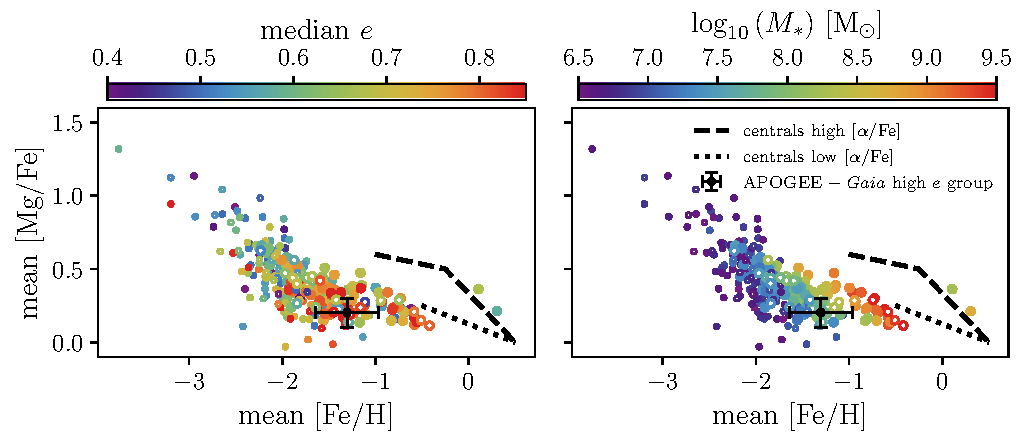
\includegraphics[width=\textwidth]{L025N752_RECAL_abundances_ecc.pdf}

\caption[The \mgfe{}-\feh{} abundances of the satellites accreted onto Milky Way mass haloes in the Recal-L025N0752 simulation of the EAGLE suite]{\label{fig:eagleabundances} Mean \mgfe{} and \feh{} of the
accreted satellites shown in Figures \ref{fig:eagle} and
\ref{fig:echange}. In both panels, point size and filling
indicate the number of particles of accreted systems, and morphology
of central galaxy, respectively, as in previous figures.  On the
right hand panel, colour denotes the masses of accreted satellites.
The same data are shown in the left hand panel, colour-coded by the
median eccentricity at $z=0$ of the debris.  The dashed and dotted
lines indicate roughly the locus of the disk stars of
MW-like central galaxies in the L025N752-Recal simulation \citep[see,
e.g.][]{2018MNRAS.477.5072M}. It is clear that the abundances of the stars in
the accreted satellites are roughly consistent with those seen in
halo stars in the APOGEE data (the median and 1$\sigma$ scatter of
the high $e$ group is shown by the black error bars).  Less massive
satellites have a large spread in \mgfe, but all have lower \feh{}
than the more massive satellites.  The increasing \feh{} with
satellite mass is very clear. The left hand panel shows that there
is a distinct lack of high eccentricity satellite debris at high
\mgfe{} and low \feh{}, such that, in general, high $e$ debris
occupies a similar locus to that of the high $e$ group in the
observed data.}

\end{figure*}

I test the numerical convergence of these results in Appendix
\ref{sec:appB}, showing that the result in Figure \ref{fig:eagle}
is robust against changes to the simulation resolution, sub-grid
model and volume. Importantly, I show that degrading the resolution
of the simulation does not significantly change the result shown
in Figure \ref{fig:echange}, which indicates that the simulations
are adequately resolving the interaction of the central galaxy and
the accreted satellite debris. It is important to emphasise that
the time at which the initial $e$ is measured is, of course, an
important factor which affects the conclusions drawn from this
result and its comparison with previous work, which we discuss 
in Section \ref{finale}.


\section{Summary and Conclusions} \label{finale}

Initially, this chapter presented an analysis of chemical compositions and orbital
information of halo stellar populations, based on APOGEE
and Gaia data. I applied k-means clustering to identify subgroups
in chemical composition and kinematics space, considering the
abundances of $\alpha$, odd-Z and Fe peak elements, and orbital
eccentricity.  I have further shown that $\sim~2/3$ of the accreted halo
stars exhibit very high orbital eccentricity and display chemical
compositions that are characteristic of those seen in massive dwarf
galaxy satellites of the Milky Way today, suggesting that this
population is likely the progeny of a single, massive accretion
event which occurred early in the history of the Milky Way Galaxy, as suggested by other groups
\citep[e.g.][]{2018MNRAS.475.1537M,2018arXiv180510288D,2018arXiv180606038H,2018MNRAS.478..611B}.
The remaining 1/3 of the sample consists of stars with low orbital
eccentricities and slightly higher abundance ratios than the high~$e$
population.  The latter stars likely result from a mixture of
different origins, including the remnants of less massive accretion
events, {\it in situ} star formation, disc heating, and likely some
contamination from the high $e$ population.

I further examined this scenario by studying a numerical simulation
from the EAGLE suite. I demonstrated that satellite galaxies accreted
into MW mass haloes show clear trends between the time of accretion
and the median eccentricity of the accreted stars at $z=0$.
According to the simulation, only satellites accreted at $z\simless
1.5$ result in median debris as high as those of the high~$e$
population identified in our data ($>0.8$). This constraint also
means that such satellites are likely to be accreted at  relatively
high stellar mass ($M_*\gtrsim 10^{8} \mathrm{M_{\odot}}$). 
A stricter constraint is obtained by comparing the median position
of high~$e$ stars with those of EAGLE accreted systems on the \mgfe{}-\feh{}
plane, whereby we infer a mass in the range $10^{8.5}-10^9~M_\odot$.
I also showed that, according to the simulation, the median
eccentricity of accreted debris generally does not appear to evolve
significantly over time, further suggesting that a high orbital
eccentricity is a good indicator of a relatively recent merger.
Analysis of the numerical simulation further suggests that a massive
accretion event such as that identified in the APOGEE/Gaia data is
not very common for a Milky Way-like galaxy, indicating an unusual
accretion history in same vein as suggested in the previous
chapters.

The high~$e$ population identified in the combined APOGEE-Gaia DR2
sample appears to be the same population as that discovered by
\citet{2018MNRAS.478..611B}, \citet{2018arXiv180510288D},
\citet{2018arXiv180606038H}, and \citet{2018ApJ...863..113H}.  I
have shown that the kinematics of the high~$e$ group is consistent
with that found in these studies, having very low, slightly negative
mean $L_z$ consistent with the \citet{2018arXiv180606038H} population,
and $r_\mathrm{ap}$ as high as 40 kpc, with a median of 15.1 kpc,
and a suggestive secondary peak at $r_\mathrm{ap} > 20$, in rough
consistency with the \citet{2018arXiv180510288D} population. The
high~$e$ population has a median eccentricity in good agreement
with those of the populations discussed by \citet{2018MNRAS.478..611B}
and the clusters measured by \citet{2018arXiv180500453M}.

Using cosmological zoom-in simulations, \citet{2018MNRAS.478..611B}
found that the growing discs of central galaxies act to radialise
the orbits or accreted satellite debris as they accrete.
This result is in seeming contradiction with our findings that
debris eccentricity is relatively unchanged after satellite accretion
(Figure~\ref{fig:echange}). However
the $e_{z_\mathrm{merge}}$ measured in these simulations is that of the
debris once the satellite is fully unbound and merged to the central
galaxy, and therefore likely already having undergone any radialisation
from its initial orbit before accretion. This result simply shows that the
orbits do not evolve greatly following accretion onto the galaxy,
and is therefore not in direct contradiction with the work of
\citet{2018MNRAS.478..611B} \citep[or][who showed a similar effect
in an earlier study]{2017MNRAS.464.2882A}. However, the finding
that the galaxies in EAGLE which do not have a significant disc
components at $z=0$ appear to follow the same trends in
$e(z=0)$-$z_\mathrm{merge}$ space (Figure \ref{fig:eagle}) suggests
that disc growth may not be the fundamental factor in driving these
trends.

\citet{2018MNRAS.tmp.1537K} suggest that the age-metallicity
distribution of the Galactic globular cluster population can be
used to infer the formation and assembly history of the Milky Way.
They identify one very massive ($M_* > 10^9\mathrm{M_\odot}$)
accretion event (\emph{Kraken}), which is associated with the
overabundance of metal-rich GCs in the accreted cluster branch of
the age-metallicity relation and has no known debris. They
argue that the \emph{Kraken} is associated with GCs that reside
within 5 kpc of the Galactic center.  \citet{2018MNRAS.tmp.1537K}
further point out that the GCs identified by \citet{2018arXiv180500453M}
(many of which are located at $r_{GC}> 10$ kpc) closely match the sample
they ascribe to the \emph{Canis Major} accretion event.
That would suggest that the discovered stellar population, as reported here would, by association, also be a part of their proposed \emph{Canis
Major} accretion event \citep[as would also be the case of the
system identified by,
e.g.,][]{2018MNRAS.478..611B,2018ApJ...852...49H,2018arXiv180606038H,
2010A&A...511L..10N}. 

In addition to these results based on simulations, it is worth
pointing out that \citet{2013MNRAS.436..122L} associated metal poor
GCs in the Milky Way with an accretion event with mass between $10^8
< M_* < 10^9\ \mathrm{M_\odot}$ (consistent with our estimation for
the high $e$ population progenitor), showing that these clusters
were on very low angular momentum orbits. In summary, all of these
results point towards confirmation that the assembly history of the
Milky Way has been very active, and quite atypical compared to other
galaxies of similar mass.

% As mentioned previously, the notion of a massive accretion event
% onto the Galaxy is not an entirely new one. The earlier
% work of \citet{2010A&A...511L..10N} and \citet{2012A&A...538A..21S}
% demonstrated that the halo divides into groups in its $\alpha$-element
% abundances, with the kinematics of the lower \afe{} group resembling
% that of an accreted population. Even earlier work by
% \citet{2003ApJ...585L.125B} showed that a low angular momentum
%  stellar population (resembling the one described in this
% paper) is present in the data used by \citet{2000AJ....119.2843C}, and possibly also in those upon which \citet{1962ApJ...136..748E}
% based their scenario for the formation of the halo.
% \citet{2003ApJ...585L.125B} suggested that this population may
% indeed be the debris of an accreted dwarf galaxy.  

% Finally, \citet{2018arXiv180606038H} suggest that the merger
% event reported in this paper and by other groups has occurred
% approximately 10~Gyr ago and was responsible for the dynamical
% heating responsible for the formation of the thick disc. The results
% from analysis of EAGLE suggest that if the debris at $e \sim 0.85$
% was accreted in a single satellite, then this is likely to have
% occurred around 8-9 Gyr ago (Figure~\ref{fig:eagle}).  The
% \citet{2018arXiv180606038H} merger time is based on the minimum
% isochronal age of the stars in their sample so it is possibly
% indicative of the final time of star formation rather than the
% actual accretion time.  On the other hand, EAGLE gives the time at
% which the satellite became bound to the central halo, so these
% timescales are potentially consistent.  Ages of stars in the Milky
% Way high \afe{} disc population are generally found to be older
% than or similar to $\sim 10$ Gyr
% \citep[e.g.][]{2013A&A...560A.109H,2016MNRAS.456.3655M,2017arXiv170600018M},
% so this does suggest that this population was in place before the
% merger occurred. It is worth mentioning, however, that analysis of
% the origin of $\alpha$-enhanced populations in EAGLE suggest that
% these stars must form in an early collapse in a period of rapid gas
% accretion, in order to foster the high density ISM necessary to
% generate a short enough gas consumption time to consume the high
% \afe{} gas into stars before it is polluted by SN Ia
% \citep{2018MNRAS.477.5072M}, rather than forming in an
% initially thin disc that was later heated. This scenario is
% consistent with the thick disc being the result of the geometric
% combination of the thick, centrally concentrated high \afe{} disc
% and the extended, flared low \afe{} disc
% \citep[e.g][]{2017arXiv170600018M,2016arXiv160901168M,2015ApJ...804L...9M}.
% Further work on this newly found halo component, and the high \afe{}
% disc, will surely shed more light on this discussion.



% \section*{Acknowledgements}

% The authors thank the anonymous reviewer for a careful and
% helpful report. We thank Marie Martig for insightful discussions
% during the preparation of this paper, and Robert Crain for crucial
% comments on a late draft of the manuscript. We also thank Vasily
% Belokurov, Lachlan Lancaster and Ryan Leaman for useful comments
% on the originally submitted mansucript. JTM acknowledges an STFC
% doctoral studentship. JP gratefully acknowledges funding from a
% European Research Council consolidator grant (ERC-CoG-646928-Multi-Pop).
% CRH acknowledges the NSF Graduate Research Fellowship through grant
% DGE-1315231. JB received support from the Natural Sciences and
% Engineering Research Council of Canada (NSERC; funding reference
% number RGPIN-2015-05235). JB also received partial support from an
% Alfred P. Sloan Fellowship. CAP is thankful to the Spanish Government
% for funding for his research through program AYA2017-86389-P. PBT
% acknowledges  Fondecyt-Conicyt Regular 1150334. This project was
% developed in part at the 2018 Gaia Sprint, hosted by the Center for
% Computational Astrophysics of the Flatiron Institute in New York
% City. This research made use of the cross-match service provided
% by CDS, Strasbourg. Analyses and plots presented in this article
% used \texttt{iPython}, and packages in the \texttt{SciPy} ecosystem
% \citep{Jones:2001aa,4160265,4160251,5725236}.  The study made use
% of high performance computing facilities at Liverpool John Moores
% University, partly funded by the Royal Society and LJMU's Faculty
% of Engineering and Technology..We acknowledge the Virgo Consortium
% for making their simulation data available.  The eagle simulations
% were performed using the DiRAC-2 facility at Durham, managed by the
% ICC, and the PRACE facility Curie based in France at TGCC, CEA,
% Bruy\`eres- le-Chatel.

% This work has made use of data from the European Space Agency (ESA)
% mission Gaia (~\url{http://www.cosmos.esa.int/gaia}), processed by
% the Gaia Data Processing and Analysis Consortium (DPAC,
% ~\url{http://www.cosmos.esa.int/web/gaia/dpac/consortium}). Funding
% for the DPAC has been provided by national institutions, in particular
% the institutions participating in the Gaia Multilateral Agreement.

% Funding for the Sloan Digital Sky Survey IV has been provided by the Alfred P. Sloan Foundation, the U.S. Department of Energy Office of Science, and the Participating Institutions. SDSS-IV acknowledges
% support and resources from the Center for High-Performance Computing at
% the University of Utah. The SDSS web site is www.sdss.org.

% SDSS-IV is managed by the Astrophysical Research Consortium for the 
% Participating Institutions of the SDSS Collaboration including the 
% Brazilian Participation Group, the Carnegie Institution for Science, 
% Carnegie Mellon University, the Chilean Participation Group, the French Participation Group, Harvard-Smithsonian Center for Astrophysics, 
% Instituto de Astrof\'isica de Canarias, The Johns Hopkins University, 
% Kavli Institute for the Physics and Mathematics of the Universe (IPMU) / 
% University of Tokyo, the Korean Participation Group, Lawrence Berkeley National Laboratory, 
% Leibniz Institut f\"ur Astrophysik Potsdam (AIP),  
% Max-Planck-Institut f\"ur Astronomie (MPIA Heidelberg), 
% Max-Planck-Institut f\"ur Astrophysik (MPA Garching), 
% Max-Planck-Institut f\"ur Extraterrestrische Physik (MPE), 
% National Astronomical Observatories of China, New Mexico State University, 
% New York University, University of Notre Dame, 
% Observat\'ario Nacional / MCTI, The Ohio State University, 
% Pennsylvania State University, Shanghai Astronomical Observatory, 
% United Kingdom Participation Group,
% Universidad Nacional Aut\'onoma de M\'exico, University of Arizona, 
% University of Colorado Boulder, University of Oxford, University of Portsmouth, 
% University of Utah, University of Virginia, University of Washington, University of Wisconsin, 
% Vanderbilt University, and Yale University.

% %%%%%%%%%%%%%%%%%%%%%%%%%%%%%%%%%%%%%%%%%%%%%%%%%%

% %%%%%%%%%%%%%%%%%%%% REFERENCES %%%%%%%%%%%%%%%%%%

% % The best way to enter references is to use BibTeX:

% \bibliographystyle{mnras}
% \bibliography{bib} % if your bibtex file is called example.bib


% % Alternatively you could enter them by hand, like this:
% % This method is tedious and prone to error if you have lots of references


% %%%%%%%%%%%%%%%%%%%%%%%%%%%%%%%%%%%%%%%%%%%%%%%%%%

% %%%%%%%%%%%%%%%%% APPENDICES %%%%%%%%%%%%%%%%%%%%%

% \appendix
% %
% \section{Modelling \mgfe{} as a function of \feh{}}
% \label{sec:appA}
% In order to test whether a change in slope is found in the relationship
% between \mgfe{} and \feh{} in the identified accreted halo groups,
% we use a Bayesian inference to fit a piecewise-linear model to the
% data. The form of the piecewise-linear function is given in
% Equation~\ref{eq:pwlin}. We follow the general procedure outlined
% in Section 7 of \citet{2010arXiv1008.4686H} for fitting models to
% data with two-dimensional uncertainties. For completeness, we
% re-iterate here the mathematics. The best fitting model is found
% by maximising the likelihood function for the parameters $O =
% [\mathrm{[Fe/H]}_0, \mathrm{[Mg/Fe]}_0, \theta_1, \theta_2]$ given
% the data, which we assume here to be of the form
% \begin{equation}
% \ln{\mathcal{L}(O|\mathrm{[Fe/H]}, \mathrm{[Mg/Fe]})} = K -
% \sum^{N}_{i=1}\left (\frac{\Delta_i^2}{2\Sigma^2_i} + \ln |\Sigma^{2}_i|\right)
% \end{equation} 
% where $\Delta_i^2$ defines the distance between the data-point $i$
% and the model, and $\Sigma^2_i$ is the variance orthogonal to the
% model, determined by the covariance matric of the data points. $K$
% is a normalisation constant, which is not necessary to consider in
% the optimisation. We assume uninformative flat priors on $\theta_{[1,2]}$,
% and allow $\mathrm{[Fe/H]}_0$ and $\mathrm{[Mg/Fe]}_0$ to be free.
% In this case, $\Delta_i^2$ is defined by
% \begin{equation}
% \label{eq:delta}
% \Delta_i^2 = \hat{\bf{v}}^T \bf{Z}_i - \it{b} \cos\theta_{[1,2]}
% \end{equation}
% where $\bf{Z}_i$ is the column vector made by (\mgfe{},\feh{}$)_i$,
% and $\hat{\bf{v}}$ is the unit vector orthogonal to the model:
% \begin{equation}
% \hat{\bf{v}} =
% \frac{1}{\sqrt{1+m_{[1,2]}^2}}\begin{bmatrix}-m_{[1,2]}\\1\end{bmatrix} =
% \begin{bmatrix}-\sin\theta_{[1,2]}\\\cos\theta_{[1,2]} \end{bmatrix}
% \end{equation}
% where $\theta_{[1,2]}$, here and in Equation \eqref{eq:delta}, is
% the angle between the linear model at that \feh{} and the x-axis,
% which is equal to $\arctan{m_{[1,2]}}$. $\Sigma^2_i$ is then simply
% defined as the projection of the data-point's covariance matrix
% $\bf{S}_i$ orthogonal to the model at that \feh{}
% \begin{equation}
% \Sigma^2_i = \hat{\bf{v}}^T \bf{S}_i \hat{\bf{v}}.
% \end{equation}
% In this case, we assume that the uncertainties on \mgfe{} and \feh{}
% are uncorrelated, such that
% \begin{equation}
% \bf{S}_i = \begin{bmatrix} \delta \mathrm{[Fe/H]}_i & 0 \\ 0 & \delta \mathrm{[Mg/Fe]}_i \end{bmatrix}
% \end{equation}
% where we use the catalogue values for the uncertainties on \feh{}
% and \mgfe{}. We minimise the negative log-likelihood using a downhill
% simplex algorithm \citep{doi:10.1093/comjnl/7.4.308}, and use this
% optimal solution to initiate an Markov Chain Monte Carlo (MCMC)
% sampling of the posterior PDF of the parameters O using an
% affine-invariant ensemble MCMC sampler \citep{goodmanweare2010} as
% implemented in the python package \texttt{emcee}
% \citep{2013PASP..125..306F}. We report the median and standard
% deviation of this posterior PDF as our best-fit parameters.

% \section{Numerical Convergence Tests}
% \label{sec:appB}
% We examine in this appendix the effect on the results presented in Figures
% \ref{fig:eagle} and \ref{fig:echange} of varying the simulation
% resolution, box-size, and subgrid model parameters, in order to
% demonstrate that these results are well converged numerically. We
% perform the equivalent analysis to that presented for L025N752-Recal
% (in the main body of the paper) on lower resolution volumes of the
% EAGLE simulations.

% \citet{2015MNRAS.446..521S} define `weakly' converged predictions
% as those which are unaffected by variation in the simulation
% resolution after re-calibrating the sub-grid physics. We test this
% by examining the equivalently sized, $L=25$ cMpc, lower resolution
% run (at a factor of 10 lower in mass than L025N752-Recal) which
% adopts the `Reference' sub-grid model, which we refer to as
% L025N376-Ref. We show the resulting equivalent of \ref{fig:eagle}
% for L025N356-Ref in \ref{fig:n356ref}. It is clear from this figure
% that the general prediction of \ref{fig:eagle} holds, in spite of
% the fact that the lower resolution simulation clearly does not
% resolve galaxies at masses as low as L025N752-Recal. The upper
% envelope of the distribution, which defines the maximum $z=0$
% eccentricity of a satellite merged at any given $z$, is still clear
% out to $z\sim5$. Given that the sub-grid feedback model is adjusted
% between the `Reference' and `Recalibrated' models to maintain the
% predictions of the former, from this we gather that the result is
% `weakly' converged.

% \begin{figure}
% 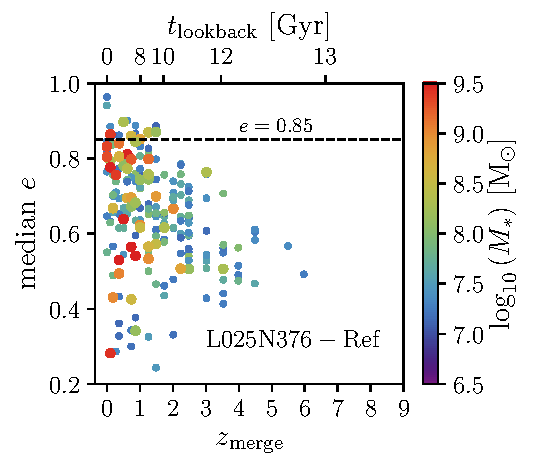
\includegraphics[width=\columnwidth]{L025N376_REF_zmerge_mediane_npart20.pdf}
% \caption{\label{fig:n356ref} The merger time $z_\mathrm{merge}$ of
% satellites accreted onto Milky Way mass haloes in the L025N356-Ref
% simulation against the median eccentricity $e$ of their stellar
% debris at $z=0$, produced via an equivalent analysis to that which
% produced Figure \ref{fig:eagle}. The trends in Figures \ref{fig:n356ref}
% and \ref{fig:eagle} are clearly conserved under an increase in
% resolution with no recalibration of the sub-grid feedback model,
% demonstrating the strong numerical convergence of these results.}
% \end{figure}

% In order to check that the prediction of EAGLE for the $z=0$
% eccentricity as a function of merger time is `strongly' converged,
% we must also ascertain that the trends in Figure \ref{fig:n356ref}
% are conserved when the resolution is increased, but the sub-grid
% model held fixed. We test this by performing an equivalent analysis
% on the L025N752-Ref model, which has a resolution equal to the
% L025N752-Recal model, but assumes the same sub-grid physics as
% L025N376-Ref. The resulting $z=0$ $e$ against merger time is shown
% in Figure \ref{fig:n752ref}. The trends which are seen in both the
% low-resolution `Reference' model (Figure \ref{fig:n356ref}) and
% high-resolution `Recalibrated' model (Figure \ref{fig:eagle} in the
% main text) are clearly conserved here also\footnote{ There is a very slight change in the exact position of the maximum of the distribution as a function of $z_\mathrm{merge}$, however, we contend that this is due to the stochastic sampling of the true underlying distribution.}, demonstrating the
% `strong' numerical convergence of these results.

% \begin{figure}
% 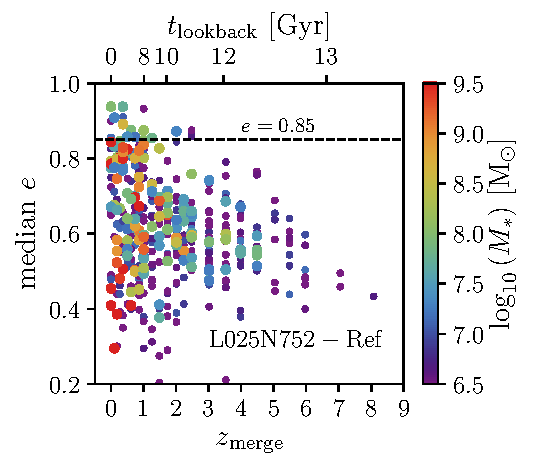
\includegraphics[width=\columnwidth]{L025N752_REF_zmerge_mediane_npart20.pdf}
% \caption{\label{fig:n752ref} The merger time $z_\mathrm{merge}$ of
% satellites accreted onto Milky Way mass haloes in the L025N752-Ref
% simulation against the median eccentricity $e$ of their stellar
% debris at $z=0$, produced via an equivalent analysis to that which
% produced Figure \ref{fig:eagle}. The upper envelope of $z=0$
% eccentricity for a given merger time is reproduced in this lower
% resolution simulation, albeit with a different calibration of the
% subgrid model, demonstrating the `weak' convergence of this result.}
% \end{figure}


% \begin{figure}
% 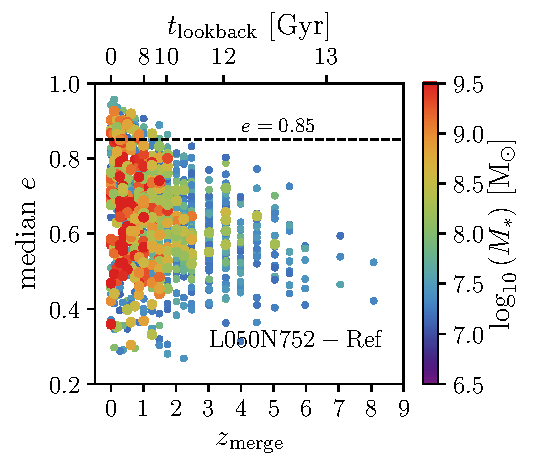
\includegraphics[width=\columnwidth]{L050N752_REF_zmerge_mediane_npart20.pdf}
% \caption{\label{fig:l50} The merger time $z_\mathrm{merge}$ against
% median eccentricity $e$ of the stellar debris at $z=0$, of the 1154
% accreted satellites (with > 20 particles) of 126 central galaxies
% from the L050N752-Ref simulation, produced via an equivalent analysis
% to that which produced Figure \ref{fig:eagle}. The trends seen in
% Figures \ref{fig:eagle}, \ref{fig:n356ref} and \ref{fig:n752ref}
% are seen again, even though a much larger sample of accretion events
% is analysed.} \end{figure}

% We also perform the analysis on a larger volume, $L=50$ cMpc, EAGLE
% simulation, which adopts the `Reference' sub-grid model at the same resolution as the smaller volume: L050N752-Ref.
% In this much larger volume, we
% track the accretion of 1154 satellites onto 126 central haloes,
% again with halo masses which are roughly equivalent to that of the
% Milky Way. The resulting distribution of satellite debris in median
% $e(z=0)$  against merger time is shown in Figure \ref{fig:l50}.
% Again, the trend between the maximum $z=0$ eccentricity and
% $z_\mathrm{merge}$ is seen, now more clearly, as a result of the
% better statistics offered by the increased sample size. This
% demonstrates that the results presented from EAGLE are strongly
% robust to variations in the simulation resolution, box-size and
% sub-grid physics.

% Finally, we show in Figure \ref{fig:echange_lowres} that the findings
% of Figure \ref{fig:echange} are robust to degradation in the
% simulation resolution. It is possible that the dynamical interaction
% between the central galaxy and the accreting satellite may be poorly
% modelled by the simulations, which are of a relatively low resolution
% \citep[as opposed to idealised simulations such as those of
% e.g.][]{2017MNRAS.464.2882A}, reducing the action of the central
% galaxy on the accreting satellites. By this reasoning, a degradation
% in the simulation resolution should decrease any changes to the
% orbital properties of the satellites, as these effects would be
% worsened. In Figure \ref{fig:echange}, showing the higher resolution
% simulation, we find the scatter around the dashed unity line to be
% 0.13. In the lower resolution we find the scatter to be comparable,
% if not slightly increased, at 0.15. As a result, we contend that
% these interactions are likely well modelled by the simulation, even
% at this relatively low resolution.

% \begin{figure}
% 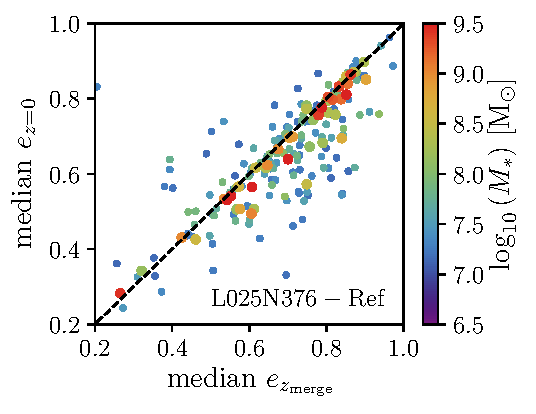
\includegraphics[width=\columnwidth]{L025N376_REF_inite_mediane_npart20.pdf}
% \caption{\label{fig:echange_lowres} The change in eccentricity between the snapshot immediately after the satellites become unbound and $z=0$ in the L025N376-Ref simulation (equivalent to Figure \ref{fig:echange} in the main text). Degrading the simulation resolution has little effect on this result, which suggests that the lack of any significant radialisation or circularisation of orbits after satellite infall is not due to poorly resolved dynamics, which would act to reduce any scatter upon degradation of the simulation resolution.  }
% \end{figure}


% %%%%%%%%%%%%%%%%%%%%%%%%%%%%%%%%%%%%%%%%%%%%%%%%%%


\chapter{Summary and Conclusions}

In the preceding chapters, I have presented novel results that provide insight into the history of the Milky Way and the nature of it. In this chapter I will attempt to combine these findings into a coherent new picture of the formation of the Milky Way, drawing also (where necessary) from the body of literature which I discussed in Chapter \ref{chapter:intro} and the introductions and concluding sections of each of the other chapters. These new insights into the evolution and resulting structure of the Galaxy will allow for a re-assessment of the question of typicality of the Milky Way, inline with the overarching goal of this thesis. 

Acting as a baseline constraint on new models for the formation of the Galaxy, Chapter \ref{chapter:apogeestruc} presented an up to date mapping of the disc of the Galaxy as a function of age, \feh{} and \afe{}. It showed that the vertical structure of the disc appears to be smooth in terms of the stellar mass contribution as a function of scale height, with no clear distinction between the high and low \afe{} populations in terms of vertical structure, confirming the same findings from SEGUE of \citet{2012ApJ...751..131B}. However, I showed that the low and high \afe{} populations have a distinct \emph{radial} structure which was hitherto unseen by SEGUE, but noted by \citet{2016ApJ...823...30B} using APOGEE data also, reviving the notion that these populations may in fact be structurally distinct, but only in the sense that the high \afe{} population is centrally concentrated, and \emph{not} distinct in a vertical sense at the solar radius - presumably by coincidence of our position in the Galaxy. 

Chapter \ref{chapter:eagle} presented a new model for the formation of bimodality in \afe{} at fixed \feh{} in galaxy discs in the EAGLE simulations. EAGLE suggests that high \afe{} stars can only be readily formed in very high density environments, where the gas consumption timescale (linked to the star formation efficiency) becomes shorter than the characteristic timescale for SN Type Ia enrichment. In order to develop a chemically distinct high \afe{} population, galaxies must undergo an early period of rapid accretion, meaning that the haloes hosting bimodal galaxies are those with the most rapid dark matter accretion between $\tau \sim 4$ to $6$ Gyr. Because of this, galaxies with \afe{} bimodality are rare in the simulation, making up only $\sim 6\%$ of Milky Way mass galaxies. This strongly suggests that the Milky Way had an atypical assembly history, which lead it to become a very atypical disc galaxy at it's stellar mass. The simulations predict that the Milky Way then should have a very centrally concentrated high \afe{} population, formed in a rapid collapse at early times, leaving a kinematic and structural distinction between it and the low \afe{} population, which is more extended and formed at late times as a cool disc. This appears to be the case, at least in terms of spatial structure, given the findings of Chapter \ref{chapter:apogeestruc}.

The prediction of an atypical accretion history for galaxies hosting a bimodality in their \afe{} distribution at fixed \feh{} in EAGLE suggests that the Milky Way should also have experienced an irregular history of accretion. I tested this prediction in Chapter \ref{chapter:highe}, demonstrating that the \emph{Gaia} DR2 data, in combination with APOGEE, reveals that the Milky Way stellar halo harbours a hitherto unseen massive accreted component, which becomes clear when orbital properties and chemical abundances are combined. I showed that in the EAGLE simulations, these accreted debris populations are extremely rare, and result from the late-time ($z\sim 1$ to $2$) accretion of relatively massive ($10^{8} < M_{*} < 10^{9}\ \mathrm{M_{\odot}}$) systems. The element abundances of the satellite debris in EAGLE agree well with those of the Milky Way debris, and further suggest that the stellar mass of the progenitor must have been in the range of $\sim 10^{8.5}\ \mathrm{M_{\odot}}$. These findings present a first insight into how the predictions of EAGLE and future simulations might be tested in the Milky Way halo.

Returning to the main goals of the thesis as outlined at the 
start of Chapter \ref{chapter:intro}, I have:
\begin{itemize}
    \item Developed a detailed and state-of-the-art picture of the present day structure and state of the Milky Way, which provides a more stringent constraint on models for its formation by directly finding the structure of the Galaxy as a function of stellar age.
    \item Shown that cosmological simulations produce galaxies with element abundance patterns consistent with those of the Milky Way, and that these galaxies are \emph{not} typical, at least compared to other disc galaxies in the stellar mass range of the Milky Way. The most fundamental aspect of this atypicality appears to be in their mass assembly histories.
    \item Tested the predictions of the cosmological simulations by reconstructing aspects of the assembly history of the Galaxy using the \emph{Gaia} DR2 and APOGEE data. I also showed that the simulations can correctly predict the element abundances of accreted satellite debris, which highlights their usefulness for future studies of satellite galaxies.
\end{itemize}
From these points of view, it would seem that the Milky Way is certainly not typical of a disc galaxy at its stellar mass, and likely had a far more active early history of mass assembly than its similarly massive siblings. This presumably lead to its structure at the present day, harbouring a centrally concentrated high \afe{} population which was formed in this early episode. The debris in the stellar halo of our Galaxy provides an excellent tool to test this prediction of an early assembly, and the results in Chapter \ref{chapter:highe} are merely a step toward the full reconstruction of the Milky Way assembly history.


\section{Future Prospects}

With the oncoming deluge of data for stars in the Milky Way, not just from the future \emph{Gaia} data releases \citep[which will include epoch spectroscopy and photometry, offering the potential to mine the data for element abundances and ages, e.g.][]{2016A&A...595A...1G}, but also from planned spectroscopic surveys (e.g. MOONS, \citeauthor{2012SPIE.8446E..0SC} \citeyear{2012SPIE.8446E..0SC}; WEAVE, \citeauthor{2012SPIE.8446E..0PD} \citeyear{2012SPIE.8446E..0PD}; and 4MOST, \citeauthor{2016SPIE.9908E..1OD} \citeyear{2016SPIE.9908E..1OD}) prospects are very strong for a more complete insight into the history of the Galaxy. Not only will improved and larger numbers of spectroscopic and astrometric information become available, but there are also a number of ongoing and planned asteroseismic surveys, such as TESS \citep{2015JATIS...1a4003R} and PLATO \citep{2017AN....338..644M}. Improvements in the data processing and our understanding of asteroseismic data from completed missions like \emph{Kepler} \citep{2010Sci...327..977B}, will also provide better measurements of stellar oscillations. Improved asteroseismology for a large number of stars over wide ranges in parameter space would generate great improvements in our estimates for stellar masses, and therefore ages, allowing for better training sets for spectroscopically measuring ages \citep[Such as those in Chapter \ref{chapter:apogeestruc}, from methods like that of e.g.][]{2016MNRAS.456.3655M}. 
% ADD CHAPTERS HERE


%% APPENDICES %%%%%%%%%%%%%%%%%%%%%%%%%%%%%%%%%%%%%%%%%%%%%%%%%%%%%%%%%%%%%%%%%%%%%%
\let\svaddcontentsline\addcontentsline
\renewcommand\addcontentsline[3]{%
  \ifthenelse{\equal{#1}{lof}}{}%
  {\ifthenelse{\equal{#1}{lot}}{}{\svaddcontentsline{#1}{#2}{#3}}}}

\appendix
\chapter{The age-resolved spatial structure of the Milky Way disk}

\section{Density Fits}
\label{sec:densityfits}
I briefly discuss the quality of the fits performed with the method outlined in section \ref{sec:methoda}. Figures \ref{fig:low_fitcomp} and \ref{fig:high_fitcomp} show the distance modulus distribution of the APOGEE DR12 data in each of the mono-age and mono-\feh{} bins (grey histograms) and the resulting distance modulus distribution when the best fit density model for each bin is run through the calculated effective selection function (which is the space in which models are fit in our procedure). The red line represents a single-exponential fit to the radial and vertical spatial distribution and the black lines give the best fit broken-exponential density model (upon which I base the results).I show the single-exponential fit in order to demonstrate that in most cases this does not provide a good fit to the data and that when a single exponential is a better fit, the broken-exponential density fit matches it.

Regarding Figure \ref{fig:low_fitcomp}, which shows the low \afe{} sub-populations, it is clear that the black curve (broken exponential) represents a far better model for the data than the red curve (single exponential), in all mono-age, mono-\feh{} bins. While the black curve is not perfect in all cases, the peak of the distribution tends to lie at the correct $\mu$, whereas the red curve finds a peak at higher $\mu$ in most cases (due to the higher than necessary density at low Galactocentric radius in this model).

 Figure \ref{fig:high_fitcomp} demonstrates the fits for the high \afe{} sub-populations. The hatched out panels reflect those with less than 30 stars, which are too noisy to render reliable fits. In many of the remaining panels, the red curve is similar or identical to the black, due to the fact that many of the high \afe{} populations are better described by single exponentials, and the broken exponential generally recovers this result. In most of the cases where the curves differ greatly, the red curve recovers the peak of the distribution better than the black - suggesting that breaks which \emph{were} fit in the radial range considered are artificial, and due to the noisy data in this regime. I discuss the broken exponential fits in the main text in order to make proper comparison with the low \afe{} sample, although it seems plausible that the single exponential model provides a better explanation of the data. 

 \begin{figure*}
      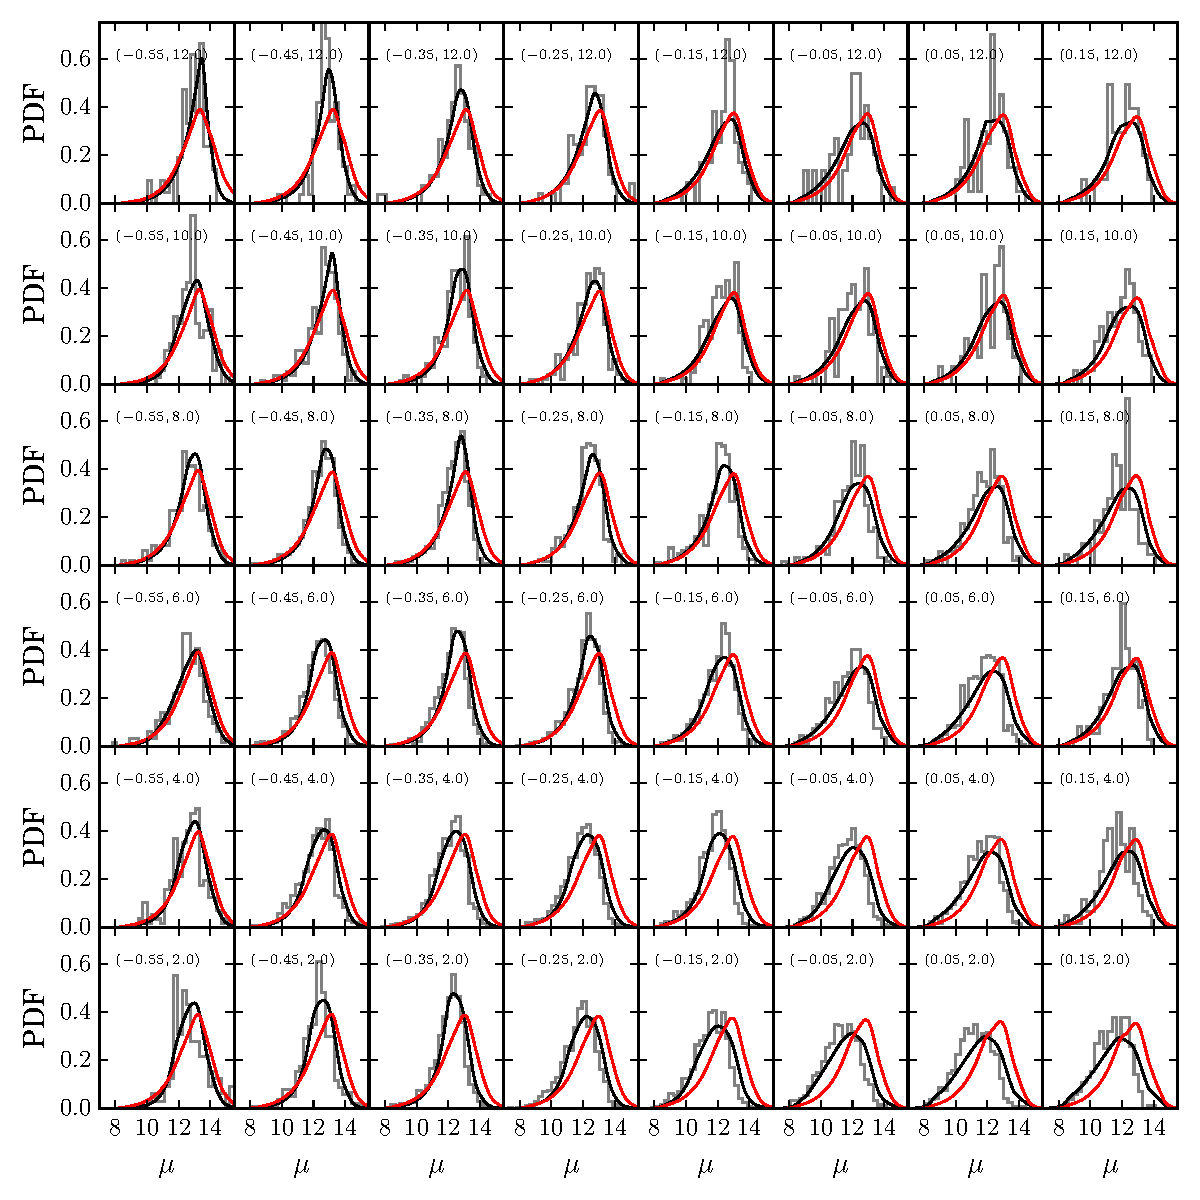
\includegraphics[width=\textwidth]{low_fitcomparison.pdf}
   \caption[Comparison between the APOGEE DR12 data and best-fit density models for the low \afe{} mono-age, mono-\feh{} populations]{ Comparison between the best fit models and the APOGEE data for mono-age, mono-\feh{} populations in the low \afe{} sub-sample. The grey histogram shows the distance modulus distribution of the APOGEE data for the mono-age, mono-\feh{} bin indicated by the (\feh{} [dex], age [Gyr]) coordinate given in each panel, where each panel shows a different mono-age, mono-\feh{} bin. The coloured curves show the distance modulus distribution found when the best fit broken exponential (black) and single exponential (red) density model is run through the effective selection function. It is clear that the broken exponential density model provides a qualitatively better fit to the data in all cases.}
     \label{fig:low_fitcomp}
 \end{figure*}

 \begin{figure*}
      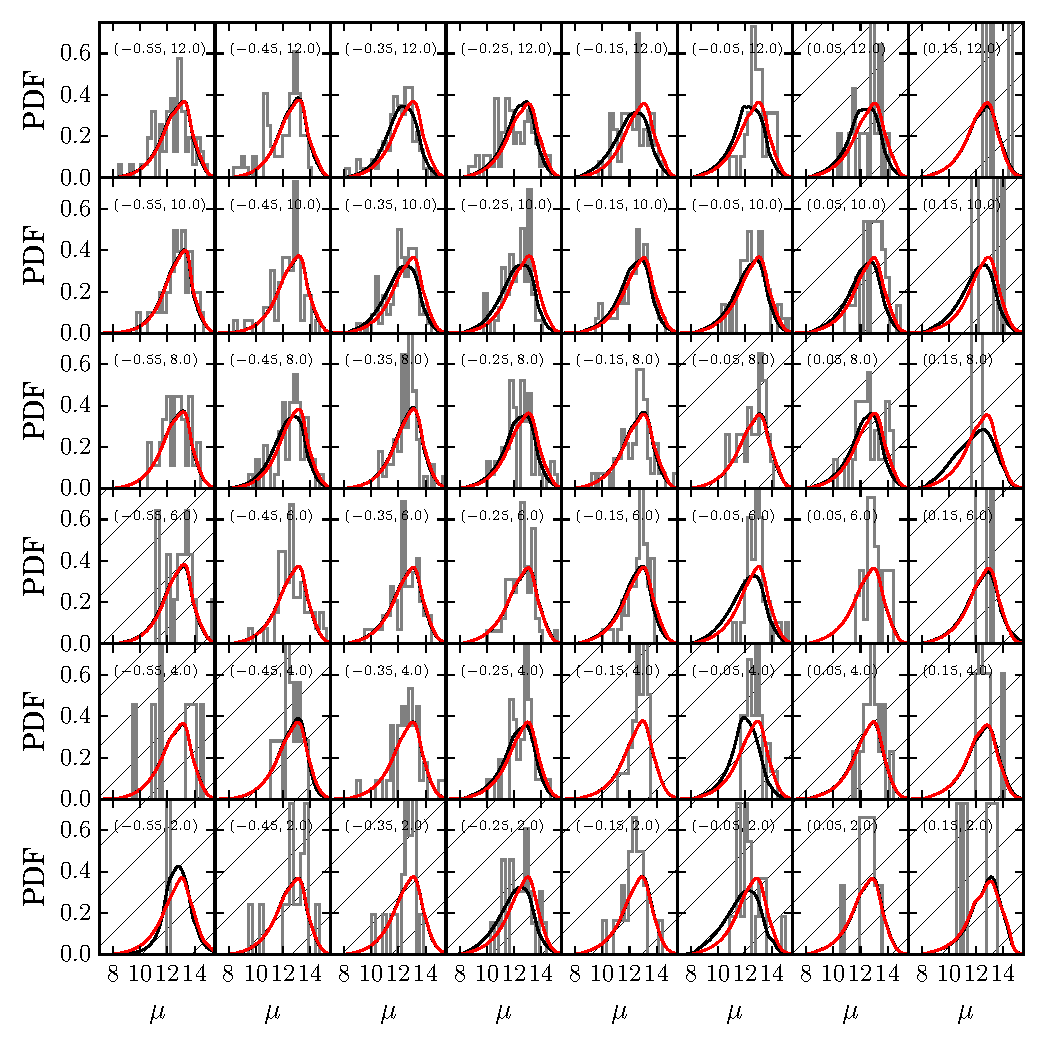
\includegraphics[width=\textwidth]{high_fitcomparison.pdf}
   \caption[Comparison between the APOGEE DR12 data and best-fit density models for the high \afe{} mono-age, mono-\feh{} populations]{Comparison between the best fit models and the APOGEE data for mono-age, mono-\feh{} populations in the high \afe{} sub-sample. Each panel again shows a different mono-age, mono-\feh{} bin. The grey histogram shows the distance modulus distribution of the APOGEE data for the mono-age, mono-\feh{} bin indicated by the (\feh{} [dex], age [Gyr]) coordinate given in each panel. The coloured curves show the distance modulus distribution found when the best fit broken exponential (black) and single exponential (red) density model is run through the effective selection function. In many cases the red and black curves are indistinguishable (only red is seen), or very similar. In cases where the black and red curves are different, the red provides a qualitatively better fit. Bins with less than 30 stars (which I disregard for the majority of the analysis and discussion) are hatched out. }
     \label{fig:high_fitcomp}
 \end{figure*}

 \section{The effect of uncertainties on trends with age}
 \label{sec:ageerror}


In order to demonstrate and characterise the effect that the age errors have on the interpretation of the trends between structural parameters and age, I use a mock data set with an input trend of $h_Z$ with age which increased monotonically with age from 0.2 to 1.2 kpc. Ages are assigned to each $h_Z$ population, sampling uniformly in bins of width 2 Gyr, to which I then added a random gaussian error of $40\%$, replicating the shifting of stars with different $h_Z$ into each age bin. In each bin, I sample a single exponential (a broken exponential with $R_\mathrm{peak}=0$) with scale length 8 kpc. This higher scale length is required to make the test computationally efficient, to produce realistic numbers of stars when selecting stars in APOGEE fields and does not impact on the results of this test. We assume no error on the stellar positions, in order to isolate the effect of the age errors. 

 \begin{figure}
      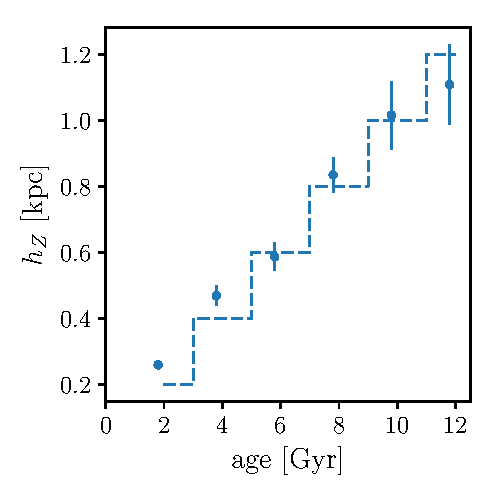
\includegraphics[width=0.5\columnwidth]{montecarlo_hz.pdf}
   \caption[Scale height vs. age for a Monte Carlo mock data set, intended to simulate the effect of age uncertainties on the trends recovered by the density fitting methodology]{The resulting age-$h_Z$ trend from the Monte Carlo sampling of a set of mock density distributions. The input  density models had $h_Z$ increasing monotonically with age (in bins of $\Delta\mathrm{age}= 2$ Gyr) from 0.2 to 1.2 kpc (shown by the \emph{blue} dashed line). After sampling of the density distribution, random errors of $40\%$ were applied to the mock ages, and the structural parameters were measured using the exact density fitting method applied to the APOGEE data. The method is able to approximately recover the general shape of the input age-$h_Z$ relation, showing a clear trend with age. The age errors increase the error bar sizes significantly where mixing does occur, but the results are consistent with the input in most cases.}
     \label{fig:montecarlo_hz}
 \end{figure}

While this test is a somewhat simplistic representation of the underlying processes, it serves as a good example of the effect of the age uncertainties which are expected in the present data. One example of its simplicity is the assignment of a single $h_Z$ to relatively wide bins in age. It seems logical to assume that if there is an age-$h_Z$ relation, then the change in $h_Z$ should be somewhat continuous with age. This test assigns the same $h_Z$ to stars at bin edges (which should have $h_Z$ close to that of the bin-edge stars in the neighbouring bin). This may artificially increase the amount of blurring of the age-$h_Z$ trend. I also simplify the test by assuming that the only changing parameter is the scale height. Realistic structural parameters would change the relative number of stars within each bin observed by APOGEE (and considered in our test), and may change the level of contamination between bins. However, this simple approximation represents a `worst case' scenario, where the mixing between bins is maximal.

I restrict the mock data to the APOGEE fields, simplifying the selection function to a distance cut (assuming the selection fraction is 1 out to a distance which corresponds to $M_\mathrm{H}= -1.5$, assuming no extinction).  I apply the method described in Section \ref{sec:methoda} to the mock data, fitting a broken exponential profile, and using the best fit solution to initiate an MCMC sampling of the posterior probability distribution. As in the main body of the paper, the reported parameter values reflect the median and $\sigma$ of one dimensional projections of the MCMC chain. The resulting age-$h_Z$ relation is shown in Figure \ref{fig:montecarlo_hz}.  A clear trend is recovered between age and $h_Z$. The trend is still recovered at high age, regardless of the high level of mixing between bins, which increases the size of the error bars. The higher-scale height components are recovered by the analysis, but results are scattered around the input values, with large error bars. This serves to show that even in the face of large age uncertainties causing mixing between the adopted bins, this method is still able to recover the underlying trends of parameters with age.


\chapter{The origin of $\alpha$-element bimodality in disk galaxies of the EAGLE simulations}

\section{Type Ia SNe Subgrid physics variations}
\label{sec:subgrid}

\begin{figure*}
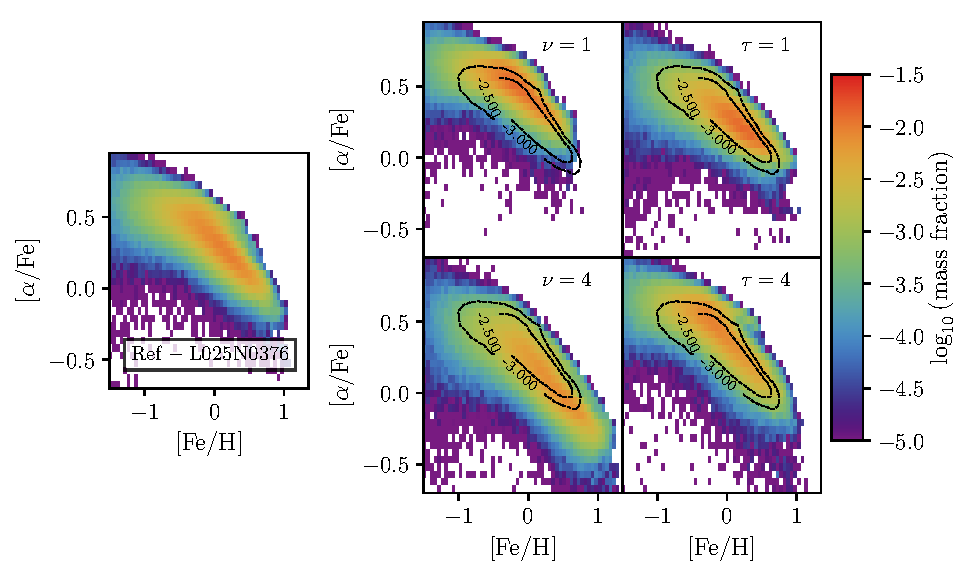
\includegraphics[width=1.\textwidth]{L0100N1504_REFERENCE_disks_4to8_SNIAsubgridvariations.pdf}
\caption[The \afe{}-\feh{} distribution of Milky Way like galaxies in L025N0376 under variations of the SNe feedback sub-grid scheme]{\label{fig:subgrid} The \afe{}-\feh{} distribution of Milky Way like galaxies in simulations of the L025N0376 volume. The left panel shows the distribution realised by the Ref-L025N0376 simulation, whilst the four panels on the right show that from simulations in which a parameter governing the number of Type SNIa per unit stellar mass formed, $\nu$, or the characteristic e-folding timescale of the Type SNIa delay function, $\tau$, has been varied. On these panels, the overlaid black contours are from the Ref-L025N0376 distribution, highlighting the significant changes to the \afe{}-\feh{} distribution induced by these parameter changes.}
\end{figure*}

I briefly examine in this appendix the degree to which variation of the subgrid parameters governing the rate of Type Ia SNe influences the \afe{}-\feh{} distribution of disc stars of Milky Way-like galaxies. I analyse four simulations that adopt the same initial conditions as the Ref-L025N0376 simulation, two of which vary the total number of Type Ia SNe per unit of initial stellar mass formed, adopting $\nu = 1\times 10^{-3}\,{\rm M}_{\odot}^{-1}$ and $\nu = 4\times 10^{-3}\,{\rm M}_{\odot}^{-1}$ (relative to the Reference model, which adopts $\nu = 2\times 10^{-3}\,{\rm M}_{\odot}^{-1}$) , and two of which vary the characteristic e-folding timescale of the Type Ia SNe delay time distribution, adopting $\tau = 1\,{\rm Gyr}$ and $\tau = 4\,{\rm Gyr}$ (where the Reference model assumes $\tau = 2\,{\rm Gyr}$).

I examine the 56 galaxies in the Ref-L025N0376 simulation with $\kappa_\mathrm{co} > 0.4$ and stellar mass in the interval $4 < M_* < 8\times10^{10}\ \mathrm{M_{\odot}}$. I identify the same haloes in the 4 variation runs using the same particle matching technique \citep{2015MNRAS.453L..58S} used to pair haloes with their counterpart in the DMONLY simulation.

The right four panels of Fig. \ref{fig:subgrid} show the \afe{}-\feh{} distribution of these galaxies in the varied simulations as 2-dimensional histograms, with the overlaid contours showing the equivalent distribution from the Reference simulation, shown in its entirety in the left panel. Varying the number of Type Ia SNe per unit stellar mass formed has a significant impact on the distribution, as changing the number of Type Ia SNe also changes the total mass of Fe synthesised per unit stellar mass formed. Decreasing (increasing) the number of Type Ia SNe therefore shifts the distribution upward (downward) to a higher (lower) \afe{}, and truncates the distribution at a lower (higher) \feh{}. The characteristic delay timescale of Type Ia SNe governs the likelihood of gas becoming enriched with the Fe synthesised by Type Ia SNe whose progenitors formed recently. A shorter (longer) delay timescale results in a greater (lesser) fraction of stars forming from Fe-rich gas, inhibiting (aiding) the formation of a high-\afe{} sequence. 

These results indicate that the parameters governing the subgrid implementation of enrichment by Type Ia SNe, which are in general rather poorly constrained, have a tangible impact on the resulting \afe{}-\feh{} distribution of disc stars. This highlights the importance of quantifying these sources of systematic uncertainty, and of ensuring that models used to examine the evolution of galaxy elemental abundances are broadly compatible with orthogonal constraints. As discussed by \citet{2015MNRAS.446..521S}, the values of $\nu$ and $\tau$ adopted by EAGLE were calibrated to ensure that the simulations broadly reproduce the observed evolution of the cosmic Type Ia SNe rate density. 


\chapter{The nature of accreted halo populations in the Milky Way}
\section{Modelling \mgfe{} as a function of \feh{}}
\label{sec:appA}
In order to test whether a change in slope is found in the relationship
between \mgfe{} and \feh{} in the identified accreted halo groups in Chapter \ref{chapter:highe},
I use a Bayesian inference to fit a piecewise-linear model to the
data. The form of the piecewise-linear function is given in
Equation~\ref{eq:pwlin}. I follow the general procedure outlined
in Section 7 of \citet{2010arXiv1008.4686H} for fitting models to
data with two-dimensional uncertainties. For completeness, I
re-iterate the mathematics here. The best fitting model is found
by maximising the likelihood function for the parameters $O =
[\mathrm{[Fe/H]}_0, \mathrm{[Mg/Fe]}_0, \theta_1, \theta_2]$ given
the data, which I assume here to be of the form
\begin{equation}
\ln{\mathcal{L}(O|\mathrm{[Fe/H]}, \mathrm{[Mg/Fe]})} = K -
\sum^{N}_{i=1}\left (\frac{\Delta_i^2}{2\Sigma^2_i} + \ln |\Sigma^{2}_i|\right)
\end{equation} 
where $\Delta_i^2$ defines the distance between the data-point $i$
and the model, and $\Sigma^2_i$ is the variance orthogonal to the
model, determined by the covariance matrix of the data points. $K$
is a normalisation constant, which is not necessary to consider in
the optimisation. I assume uninformative, flat priors on $\theta_{[1,2]}$,
and allow $\mathrm{[Fe/H]}_0$ and $\mathrm{[Mg/Fe]}_0$ to be free.
In this case, $\Delta_i^2$ is defined by
\begin{equation}
\label{eq:delta}
\Delta_i^2 = \hat{\bf{v}}^T \bf{Z}_i - \it{b} \cos\theta_{[1,2]}
\end{equation}
where $\bf{Z}_i$ is the column vector made by (\mgfe{},\feh{}$)_i$,
and $\hat{\bf{v}}$ is the unit vector orthogonal to the model:
\begin{equation}
\hat{\bf{v}} =
\frac{1}{\sqrt{1+m_{[1,2]}^2}}\begin{bmatrix}-m_{[1,2]}\\1\end{bmatrix} =
\begin{bmatrix}-\sin\theta_{[1,2]}\\\cos\theta_{[1,2]} \end{bmatrix}
\end{equation}
where $\theta_{[1,2]}$, here and in Equation \eqref{eq:delta}, is
the angle between the linear model at that \feh{} and the x-axis,
which is equal to $\arctan{m_{[1,2]}}$. $\Sigma^2_i$ is then simply
defined as the projection of the data-point's covariance matrix
$\bf{S}_i$ orthogonal to the model at that \feh{}
\begin{equation}
\Sigma^2_i = \hat{\bf{v}}^T \bf{S}_i \hat{\bf{v}}.
\end{equation}
In this case, I assume that the uncertainties on \mgfe{} and \feh{}
are uncorrelated, such that
\begin{equation}
\bf{S}_i = \begin{bmatrix} \delta \mathrm{[Fe/H]}_i & 0 \\ 0 & \delta \mathrm{[Mg/Fe]}_i \end{bmatrix}
\end{equation}
where I use the APOGEE catalogue values for the uncertainties on \feh{}
and \mgfe{}. I minimise the negative log-likelihood using a downhill
simplex algorithm \citep{doi:10.1093/comjnl/7.4.308}, and use this
optimal solution to initiate an Markov Chain Monte Carlo (MCMC)
sampling of the posterior PDF of the parameters O using an
affine-invariant ensemble MCMC sampler \citep{goodmanweare2010} as
implemented in the python package \texttt{emcee}
\citep{2013PASP..125..306F}. Finally, I report the median and standard
deviation of this posterior PDF as the best-fit parameters.

\section{Numerical Convergence Tests}
\label{sec:appB}
I examine in this appendix the effect on the results presented in Figures
\ref{fig:eagle} and \ref{fig:echange} of varying the simulation
resolution, box-size, and subgrid model parameters, in order to
demonstrate that these results are well converged numerically. I
perform the equivalent analysis to that presented for Recal-L025N752
(in the main body of the paper) on lower resolution volumes of the
EAGLE simulations.

\citet{2015MNRAS.446..521S} define `weakly' converged predictions
as those which are unaffected by variation in the simulation
resolution after re-calibrating the sub-grid physics. I test for this level of convergence
by examining the equivalently sized, $L=25$ cMpc, lower resolution
run (at a factor of 10 lower in mass than Recal-L025N752) which
adopts the `Reference' sub-grid model, which I refer to as
Ref-L025N376. The resulting equivalent of \ref{fig:eagle}
for Ref-L025N356 is shown in \ref{fig:n356ref}. It is clear from this figure
that the general prediction of \ref{fig:eagle} holds, in spite of
the fact that the lower resolution simulation clearly does not
resolve galaxies at masses as low as Recal-L025N752. The upper
envelope of the distribution, which defines the maximum $z=0$
eccentricity of a satellite merged at any given $z$, is still clear
out to $z\sim5$. Given that the sub-grid feedback model is adjusted
between the `Reference' and `Recalibrated' models to maintain the
predictions of the former, from this I conclude that the result is
`weakly' converged.

\begin{figure}
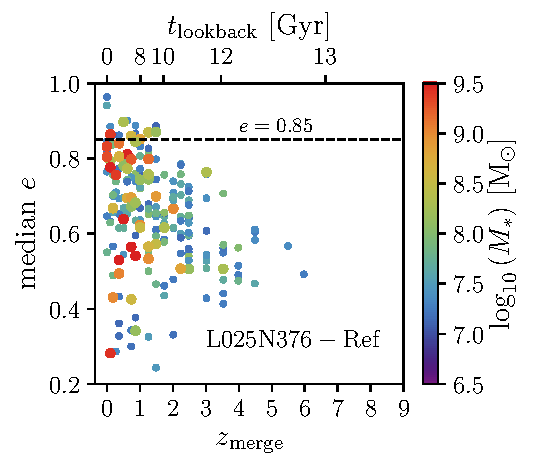
\includegraphics[width=0.5\columnwidth]{L025N376_REF_zmerge_mediane_npart20.pdf}
\caption[A recreation of Figure \ref{fig:eagle} for haloes in the Ref-L025N356 simulation]{\label{fig:n356ref} The merger time $z_\mathrm{merge}$ of
satellites accreted onto Milky Way mass haloes in the Ref-L025N356
simulation against the median eccentricity $e$ of their stellar
debris at $z=0$, produced via an equivalent analysis to that which
produced Figure \ref{fig:eagle}. The trends in Figures \ref{fig:n356ref}
and \ref{fig:eagle} are clearly conserved under an increase in
resolution with no recalibration of the sub-grid feedback model,
demonstrating the strong numerical convergence of these results.}
\end{figure}

In order to check that the prediction of EAGLE for the $z=0$
eccentricity as a function of merger time is `strongly' converged,
it is also necessary to ascertain that the trends in Figure \ref{fig:n356ref}
are conserved when the simulation resolution is increased, but the sub-grid
model held fixed. I test this by performing an equivalent analysis
on the Ref-L025N752 model, which has a resolution equal to the
Recal-L025N752 model, but assumes the same sub-grid physics as
Ref-L025N376. The resulting $z=0$ $e$ against merger time is shown
in Figure \ref{fig:n752ref}. The trends which are seen in both the
low-resolution `Reference' model (Figure \ref{fig:n356ref}) and
high-resolution `Recalibrated' model (Figure \ref{fig:eagle} in the
main text) are clearly conserved here also\footnote{ There is a very slight change in the exact position of the maximum of the distribution as a function of $z_\mathrm{merge}$, however, I contend that this is due to the stochastic sampling of the true underlying distribution.}, demonstrating the
`strong' numerical convergence of these results.

\begin{figure}
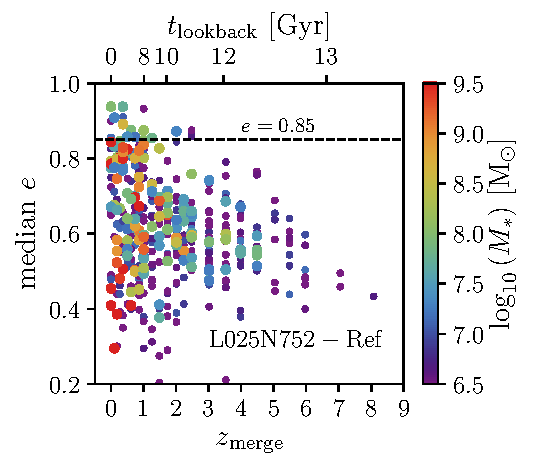
\includegraphics[width=0.5\columnwidth]{L025N752_REF_zmerge_mediane_npart20.pdf}
\caption[The equivalent of Figure \ref{fig:eagle} for haloes in the Ref-L025N752 simulation]{\label{fig:n752ref} The merger time $z_\mathrm{merge}$ of
satellites accreted onto Milky Way mass haloes in the Ref-L025N752
simulation against the median eccentricity $e$ of their stellar
debris at $z=0$, produced via an equivalent analysis to that which
produced Figure \ref{fig:eagle}. The upper envelope of $z=0$
eccentricity for a given merger time is reproduced in this lower
resolution simulation, albeit with a different calibration of the
subgrid model, demonstrating the `weak' convergence of this result.}
\end{figure}


\begin{figure}
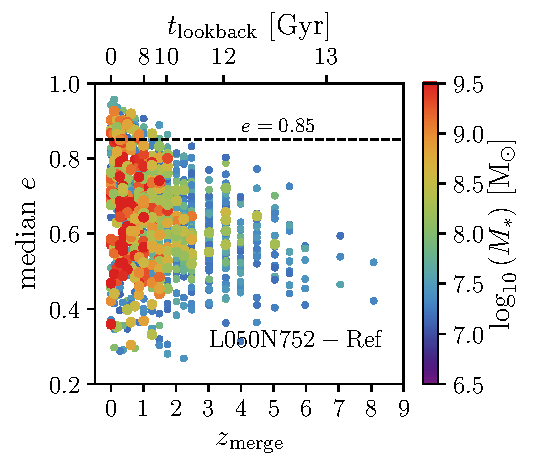
\includegraphics[width=0.5\columnwidth]{L050N752_REF_zmerge_mediane_npart20.pdf}
\caption[The equivalent of Figure \ref{fig:eagle} for haloes in the Ref-L050N752 simulation]{\label{fig:l50} The merger time $z_\mathrm{merge}$ against
median eccentricity $e$ of the stellar debris at $z=0$, of the 1154
accreted satellites (with $> 20$ particles) of 126 central galaxies
from the Ref-L050N752 simulation, produced via an equivalent analysis
to that which produced Figure \ref{fig:eagle}. The trends seen in
Figures \ref{fig:eagle}, \ref{fig:n356ref} and \ref{fig:n752ref}
are seen again, even though a much larger sample of accretion events
is analysed.} \end{figure}

I also perform the analysis on a larger volume, $L=50$ cMpc, EAGLE
simulation, which adopts the `Reference' sub-grid model at the same resolution as the smaller volume: Ref-L050N752.
In this much larger volume, I
track the accretion of 1154 satellites onto 126 central haloes,
again with halo masses which are roughly equivalent to that of the
Milky Way. The resulting distribution of satellite debris in median
$e(z=0)$  against merger time is shown in Figure \ref{fig:l50}.
Again, the trend between the maximum $z=0$ eccentricity and
$z_\mathrm{merge}$ is seen, now more clearly, as a result of the
better statistics offered by the increased sample size. This
demonstrates that the results presented from EAGLE are strongly
robust to variations in the simulation resolution, box-size and
sub-grid physics.

Finally, I show in Figure \ref{fig:echange_lowres} that the findings
of Figure \ref{fig:echange} are robust to degradation in the
simulation resolution. It is possible that the dynamical interaction
between the central galaxy and the accreting satellite may be poorly
modelled by the simulations, which are of a relatively low resolution
\citep[as opposed to idealised simulations such as those of
e.g.][]{2017MNRAS.464.2882A}, reducing the action of the central
galaxy on the accreting satellites. By this reasoning, a degradation
in the simulation resolution should decrease any changes to the
orbital properties of the satellites, as these effects would be
worsened. In Figure \ref{fig:echange}, showing the higher resolution
simulation, I find the scatter around the dashed unity line to be
0.13. At the lower resolution adopted by Ref-L025N376, I find the scatter to be comparable,
if not slightly increased - at 0.15. As a result, I contend that
these interactions are likely well modelled by the simulation, even
at this relatively low resolution.

\begin{figure}
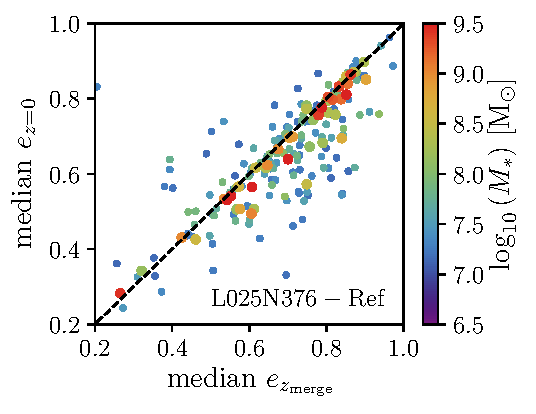
\includegraphics[width=0.5\columnwidth]{L025N376_REF_inite_mediane_npart20.pdf}
\caption[A recreation of Figure \ref{fig:echange} using satellites accreted onto Milky Way mass haloes in the lower resolution Ref-L025N376 simulation]{\label{fig:echange_lowres} The change in eccentricity between the snapshot immediately after the satellites become unbound and $z=0$ in the L025N376-Ref simulation (equivalent to Figure \ref{fig:echange} in the main text). Degrading the simulation resolution has little effect on this result, which suggests that the lack of any significant radialisation or circularisation of orbits after satellite infall is not due to poorly resolved dynamics, which would act to reduce any scatter upon degradation of the simulation resolution.  }
\end{figure}


%ADD APPENDICES HERE





%% BACK MATTER %%%%%%%%%%%%%%%%%%%%%%%%%%%%%%%%%%%%%%%%%%%%%%%%%%%%%%%%%%%%
\newpage
\addtocontents{toc}{\protect\vspace{12pt}}  % Add some vertical space
\addcontentsline{toc}{chapter}{Bibliography}
\bibliographystyle{mnras}
\bibliography{bib}





\end{document}



